\documentclass{svjour3}
\usepackage{times}
\usepackage{blindtext, graphicx}

\usepackage{colortbl}
\usepackage{tikz}
\usepackage{microtype}
\def\firstcircle{(90:1.75cm) circle (2.5cm)}
\def\secondcircle{(210:1.75cm) circle (2.5cm)}
\def\thirdcircle{(330:1.75cm) circle (2.5cm)}
\smartqed

\usepackage{balance}
\definecolor{Gray}{rgb}{0.88,1,1}
\definecolor{Gray}{gray}{0.85}
\definecolor{lightgray}{gray}{0.8}
\setlength{\tabcolsep}{0.2em}


\usepackage{subfig} 



\usepackage{amsmath}
\DeclareMathOperator*{\argmin}{argmin}

\usepackage[framed]{ntheorem}
\usepackage{framed}
\usepackage{tikz}
\usetikzlibrary{shadows}
\theoremclass{Lesson}
\theoremstyle{break}

% inner sep=10pt,
\tikzstyle{thmbox} = [rectangle, rounded corners, draw=black,
fill=Gray!20,  drop shadow={fill=black, opacity=1}]
\newcommand\thmbox[1]{%
    \noindent\begin{tikzpicture}%w
    \node [thmbox] (box){%
        \begin{minipage}{.94\textwidth}%
        \vspace{-3mm}#1\vspace{-3mm}%
        \end{minipage}%
    };%
    \end{tikzpicture}}

\let\theoremframecommand\thmbox
\newshadedtheorem{lesson}{Finding}
\newcommand{\quart}[4]{\begin{picture}(80,4)%1
    {\color{black}\put(#3,2){\circle*{4}}\put(#1,2){\line(1,0){#2}}}\end{picture}}

\newcommand{\review}[1]{{\textit{#1}}~\\}
\newcommand{\todo}[1]{\textbf{\color{red}{#1}}}
\newcommand{\respto}[1]{
\fcolorbox{black}{black!15}{
\label{response:#1}
\bf
  \scriptsize R-{#1}}~
}
\newcommand{\citeresp}[1]{
{\bf (see } \fcolorbox{black}{black!15}{
 \bf
  \scriptsize R-{#1}}~{\bf{on page \pageref{response:#1})}}
}

%% space saving measures
% \usepackage[shortlabels]{enumitem}  
% \usepackage{url}

\begin{document}

\title{How to Read Less: On the Benefit of Active Learning for Primary Study Selection in Systematic Literature Reviews%\thanks{Grants or other notes
%about the article that should go on the front page should be
%placed here. General acknowledgments should be placed at the end of the article.}
}
% \subtitle{Do you have a subtitle?\\ If so, write it here}


% \pagenumbering{arabic} %XXX delete before submission

\author{Zhe Yu         \and
        Nicholas A. Kraft \and 
        Tim Menzies%etc.
}

%\authorrunning{Short form of author list} % if too long for running head

\institute{Zhe Yu \at
              Department of Computer Science, North Carolina State University, Raleigh, NC, USA \\
              \email{zyu9@ncsu.edu}           %  \\
%             \emph{Present address:} of F. Author  %  if needed
           \and
           Nicholas A. Kraft \at
              ABB Corporate Research, Raleigh, NC, USA\\
              \email{nicholas.a.kraft@us.abb.com}
            \and
           Tim Menzies \at
              Department of Computer Science, North Carolina State University, Raleigh, NC, USA \\
              \email{tim.menzies@gmail.com}
}

% \date{Received: date / Accepted: date}

\maketitle

\begin{abstract}
  
Systematic literature reviews (SLRs) are the primary method for aggregating and synthesizing evidence in evidence-based software engineering (SE). Primary study selection is a critical and time-consuming SLR step in which reviewers use
titles, abstracts, or even full texts to evaluate thousands of studies to find the dozens of them that are relevant to the research questions. We seek to reduce the effort of primary study selection in SE SLRs by exploring and refactoring the state-of-the-art active learning techniques from evidence-based medicine and legal electronic discovery. By refactoring those methods, we discovered FASTREAD, which is a new state-of-the-art in active learning for SE SLRs. When tested on four datasets generated from existing SE SLRs of Hall, Wahono, Radjenovi{\'c}, Kitchenham et al., FASTREAD outperformed the current state-of-the-art methods. Our results show that FASTREAD can save researchers much time during
 the literature review process (since they will need to review hundreds to thousands fewer abstracts ) 
 while sacrificing very little
in the final recall  (5\%).

\keywords{Active Learning\and Systematic Literature Review\and Software Engineering\and Primary Study Selection}

\end{abstract}



\section{Introduction}
\label{sect: Introduction}

The number of new publications every year is growing rapidly. For example, on defect
prediction, 729 studies were published on IEEE
Xplore\footnote{http://ieeexplore.ieee.org} during the year of 2005 while 1,564
studies were published during the year of 2015.
Given this increasingly faster pace of software engineering (SE) research,
it has become harder and harder to remain current with
the state-of-the-art research in software engineering.


\begin{figure*}[t]
    \centering
    \subfloat[Most Difficult Aspects of SLR Process.]
    {
        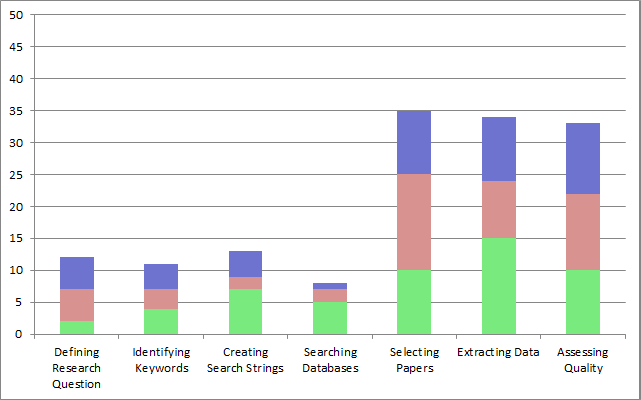
\includegraphics[width=0.48\linewidth]{difficulty.png}
        \label{fig: difficult}
    }
    \subfloat[Most Time Consuming Aspects of SLR Process.]
    {
        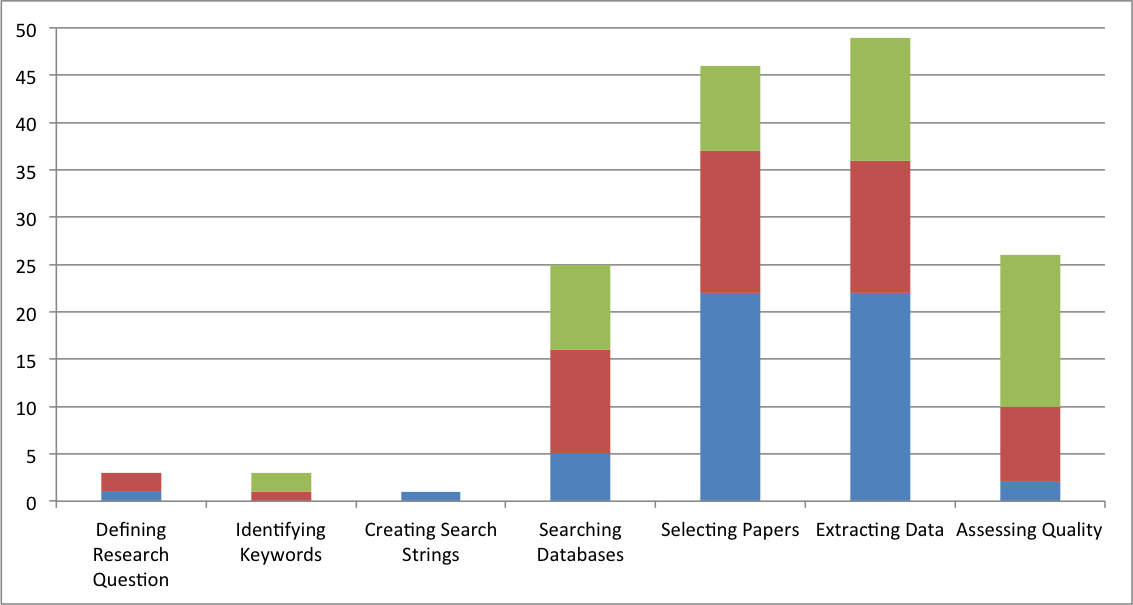
\includegraphics[width=0.48\linewidth]{time.png}
        \label{fig: time}
    }    
    \caption{Data collected from surveys to SLR authors~\cite{carver2013identifying}. Measured by number of votes, where {\setlength{\fboxsep}{1pt}\colorbox{green!40}{green}}, {\setlength{\fboxsep}{1pt}\colorbox{red!30}{red}}, and {\setlength{\fboxsep}{1pt}\colorbox{blue!50}{blue}} are number of times voted as most, second most, and third most, respectively.}
    \label{fig:barrier}
\end{figure*}
Systematic Literature Reviews
(SLRs) are one approach to this problem. SLRs are a well established and widely
applied review method in Software Engineering since Kitchenham, Dyb{\^{a}}, and
J{\o}rgensen first adopted it to support evidence-based software engineering in
2004 and 2005~\cite{kitchenham2004evidence,1377125}. 
Researchers can get a
general idea of current activity in their field of interests by reading the SLR
studies. Furthermore, a
deeper understanding of the topic may be gained by conducting an SLR.

An increasing number of SLRs has been conducted since the proposal and
revision of the SLR guidelines by Kitchenham in 2007~\cite{keele2007guidelines}. For
example, there were 26 SLRs on IEEE Xplore during the year of 2005 and that
number has increased to 137,199 for the years   2010,2015 (respectively). Various scholars  suggest that an SLR is required before any research in Software
Engineering is conducted~\cite{keele2007guidelines}.
While this is certainly a good advice,
currently an SLR is
a large, time consuming and complex
task~\cite{hassler2016identification,hassler2014outcomes,carver2013identifying,bowes2012slurp}.

Cost reduction in SLRs is therefore an important topic and will benefit researchers in software engineering community.
Previously we have analyzed the costs of SLRs~\cite{hassler2014outcomes,carver2013identifying}. As shown in Fig.~\ref{fig:barrier}, primary study selection, which is noted as ``selecting papers'' in Fig.~\ref{fig:barrier}, is among the top three most difficult
as well as time-consuming aspects in an SLR. Usually, reviewers need to evaluate
thousands of studies trying to find dozens of them that are relevant to the
research questions based on their title, abstract, or full text~\cite{bowes2012slurp}. An extreme
example of this is where reviewers sourced over
3,000 studies, and only used 7 of them in their final review~\cite{bezerra2009systematic}. The cost associated with primary study selection has become a serious problem and will continue to grow in the near future as the population of candidates for primary
studies increases dramatically. In this paper, we focus on reducing cost in primary study selection only. We prioritize primary study selection because there exists tool support for other time-consuming aspects such as searching databases~\cite{Molleri:2015:SWA:2745802.2745825,hernandes2012using}, extracting data\cite{Molleri:2015:SWA:2745802.2745825,hernandes2012using,fernandez2010slr,bowes2012slurp}, assessing quality~\cite{fernandez2010slr,bowes2012slurp,Molleri:2015:SWA:2745802.2745825}; and machine learning methods are promising in cost reduction for primary study selection~\cite{wallace2010semi,grossman2013}.

There are three main aspects in primary study selection: \textbf{(1)} retrieving initial list of primary studies, \textbf{(2)} excluding irrelevant studies, \textbf{(3)} including missing studies. We focus on excluding irrelevant studies because \textbf{a)} there already exists techniques and tools to facilitate \textbf{(1)} and \textbf{(3)} such as Snowballing~\cite{jalali2012systematic} and StArt~\cite{hernandes2012using}; \textbf{b)} the performance of excluding irrelevant studies can be evaluated using existing SLR publications.

In the SE research community, linear manual review, which requires reviewer to review every candidate study, is still the standard approach for primary study selection~\cite{kitchenham2013systematic}. On the other hand, machine learning algorithms, especially active learning, have been intensively studied to solve similar problems in other fields outside the SE research community in evidence-based medicine~\cite{paynter2016epc,wallace2010semi,wallace2010active} and in
legal electronic discovery~\cite{cormack2014evaluation,cormack2015autonomy}. This paper:
\begin{itemize}
\item
Reviews those methods. We find that in evidence-based medicine and legal electronic discovery, there are three widely recognized state-of-the-art active learning methods~\cite{cormack2014evaluation,wallace2010semi,miwa2014reducing}.
\item
Those three methods are assembled from four lower-level techniques including a) when to start training; b) query strategy; c) when/whether to stop training; d) data balancing. By analyzing techniques applied in the three methods, we generate 32 possible treatments.
\item
This paper explores all 32 treatments using data taken from the SE literature. Each treatment is evaluated by ``work saved over sampling at 95\% recall'' (WSS@95)~\cite{cohen2011performance}. 
\item
We find that one of those treatments, which we will call FASTREAD, robustly achieves the highest rank of performance across every dataset.
\end{itemize}
Interestingly, the FASTREAD treatment is not one of those used
in~\cite{cormack2014evaluation,wallace2010semi,miwa2014reducing}-- which is to say that the SE literature has nuanced differences to other kinds of literature and we should not just blindly
apply methods from other fields without certifying them on local data.
Using FASTREAD, hundreds to thousands of abstract reviewing can be avoided by sacrificing 5\% recall. That is, FASTREAD can dramatically reduce the cost of primary study selection in SE SLRs.

To assess those 32 treatments,
we need some ``gold sets'',
on which we can compare different combinations. Fortunately, in the arena of software engineering, there exist very prominent ``gold sets'' as published SLRs. This paper used three  primary study selection datasets by using the search strings and final inclusion list in such SLRs: Wahono et al. 2015~\cite{wahono2015systematic}, Hall et
al. 2012~\cite{hall2012systematic}, and Radjenovi{\'c} et al. ~\cite{radjenovic2013software}. These three SLRs are arbitrarily chosen from the set of SLR publications which define their work in enough details for us to construct datasets for simulations. Besides the three synthetic datasets, one set from Kitchenham et al. 2010~\cite{kitchenham2010systematic} has also been provided for the simulations. More details about the ``gold
sets'' will be presented later in Section~\ref{sect: datasets}. Using
these ``gold sets'', we ask and answer the following three research questions:

\begin{itemize}


\item
{\bf RQ1: Can active learning techniques reduce cost in primary study selection?} First of all, the effectiveness of active learning should be tested against traditional linear review. The rest of the research questions should not be investigated until active learning has been proved to be useful for cost reduction in primary study selection.

\item
{\bf RQ2: Should we just adopt the state-of-the-art treatments from other fields? Is it possible to build a better one by mixing and matching from those?} Active learning methods have been explored in other fields. Each of the state-of-the-art methods has its own advantage and thereby a better method might be derived by mixing and matching from those. 

\item
{\bf RQ3: How much effort can FASTREAD, our new state-of-the-art method for primary study selection, save in an SLR?} Details should be provided so that reviewers can decide whether to use FASTREAD or not.


\end{itemize}
The main contributions of this paper are:
\begin{itemize}
\item
  A demonstration of the value of  machine learning techniques for assisting primary study selection in SE SLRs.
\item
  The development of FASTREAD, a new state-of-the-art active learning method for primary study selection in SE SLRs, by refactoring three state-of-the-art methods from evidence-based medicine and electronic discovery.
  
\item
  The evaluation of our new method. The experiments shown below indicate that FASTREAD saves large amount of review efforts on primary study selection.
\item The development of a simple tool to implement FASTREAD for primary study selection.
  This tool is explained in Section~\ref{sect: tool} and is
  available for download on GitHub\footnote{https://github.com/fastread/src}. 
\end{itemize}










\section{Frequently Asked Questions}
\label{sect: Frequently Asked Questions}

When we discuss FASTREAD with our colleagues, several issues are commonly raised. This section discusses these issues.

\subsection{What about the other costs associated with SLRs?}

Our focus on the cost reductions of primary study selection is not to discount the effort associated with other parts of the SLR process. As mentioned in our introduction, we focus here on primary study selection since our data (from Fig.~\ref{fig:barrier}) indicates that this is a major component of SLR cost. 

In addition, there are tools support other components of SLRs and techniques facilitating primary study selection in different approaches. All these techniques (such as Quasi-Gold Standard based search~\cite{zhang2011empirical,zhang2011identifying}, visual text mining~\cite{Felizardo:2014:VAA:2601248.2601252,felizardo2012visual,felizardo2010approach,malheiros2007visual}, and snowballing~\cite{wohlin2014guidelines,jalali2012systematic}) are compatible and a better performance is expected when applied together. This leads to a direction of future work in which the best setting to integrate different techniques will be explored.

\subsection{What is missed?}

Our results will show, with FASTREAD, $95\%$ of the ``relevant'' studies can be retrieved by reviewing a small portion (usually hundreds of studies) of long candidate study list. Given that, it is wise to reflect
on the 5\% of papers {\em not} found by such an analysis. To this end, we took one of our case studies and reflected on:
\begin{itemize}
\item The set of papers $P_0$ that a human analyst declared to be ``relevant'' (as listed in their reference list at the end of their paper);
\item The {\em tangentially relevant} subset of those  papers $P_1 \subseteq P_0$ that a human analyst explicitly mentions, however briefly, in the body of their paper;
\item The yet smaller subset of those papers $P_2 \subseteq P_1$  that a human analyst discusses, at length, in the body of their report (and for
our purposes ``at length'' will be ``more that two lines''). We call these {\em insightful papers}. Clearly, FASTREAD should not be recommended if our method always misses the insightful papers, 
\end{itemize}
For the case studies shown below, on 30 repeats of our methods, we found that $|P_2|=0$; i.e. FASTREAD never missed an insightful paper. As for the tangentially
relevant papers, FASTREAD found all of those in 95\% of the 30 repeats. 
Based on this analysis, we infer that missing  $15\%$ of the papers is not a major impediment to using FASTREAD. Similar conclusion was derived by Shemilt et al. in 2016~\cite{shemilt2016use}.

That said, it is still true that if the SLR conductor does not want to miss any potential relevant study, he or she need to review all the candidate studies with full cost. We are actively exploring possibilities to mitigate or compensate the missing studies issue. 

% Data imbalance is explored further in Fioravanti and Nesi
% [[43]] and Zhang et al..

% Nikora and Munson [[126]] says that “without a widely agreed definition of severity
% we cannot reason about it” and Ostrand et al.
 

\subsection{What about domain knowledge?}

In our simulations, we assume that no initial seed training set is available thus a random sampling is performed to collect the minimum training set. This assumption represents the worst case while no external knowledge is available. We show in this work that the absence of that domain knowledge is not a critical failing of the approach. On the other hand, such domain knowledge usually exists in real world SLRs and will boost the performance of FASTREAD if wisely used. For example, if one relevant example and one irrelevant example are known in the very beginning, the random sampling step of FASTREAD is no longer needed and thus leads to additional cost reduction. More details about how to wisely use domain knowledge to boost FASTREAD will be explored further after this work. While we have some preliminary results in that area, we have nothing definitive to report at this time.

\subsection{What about real human reviewers?}

In our simulations, we assume that there is only one reviewer who never make mistakes. In real world SLRs, there will be multiple reviewers who make some mistakes. 

First, consider we have multiple reviewers but no mistakes. The schema of FASTREAD can be changed to one central learner with multiple review agents. Every agent reviews different studies and feedback his or her decisions to the central learner. The central learner then trains on the feedback of every agent and assigns studies to each agent for review. Such schema will keep all the property of single reviewer FASTREAD and performs similarly. In addition, there might be more intelligent way to allocate review tasks based on the different performance of review agents. Such possibility is worth exploring in future works and there already exists some studies on this topic in evidence-based medicine~\cite{wallace2011should}.

Second, consider those multiple reviewers now make mistakes. Candidate studies need to be reviewed by multiple reviewers in case any of them makes mistakes. To explore this issue, appropriate data need to be collected on how human reviewers make mistakes. Wallace et al. addressed this issue in~\cite{nguyen2015combining} by analyzing the best policy for allocating review tasks to reviewers with different experience levels as well as difference costs. We also plan to to address this issue in our future work.


\subsection{What about multiple categories of studies?}

In our simulations, we assume that the target is binary classification. However, primary study selection in real world SLRs might be a multi-label classification problem. For example, an SLR with two research questions might go through a primary study selection while each candidate is labeled as ``relevant to RQ1'', ``relevant to RQ2'', or ``irrelevant'' while the first two labels can co-exist. The simplest solution for this is to run multiple FASTREAD learners each learns on one label vs. others and each reviewer classify on one label only. In this case, the multi-label classification problem can be divided into multiple FASTREAD problems. Additional work such as ensemble learners can be explored in future works.

In summary, FASTREAD is an in-development technique that can be applied if the above trade-offs are acceptable. It can still be improved to further reduce cost of primary study selection and we will keep working on the issues until it becomes a reliable tool for different scenarios of SLRs.

























\section{Large Scale Literature Studies in SE}
\label{sect: Background}

\begin{figure}[t]
    \centering
    \begin{minipage}[t]{.51\linewidth}
    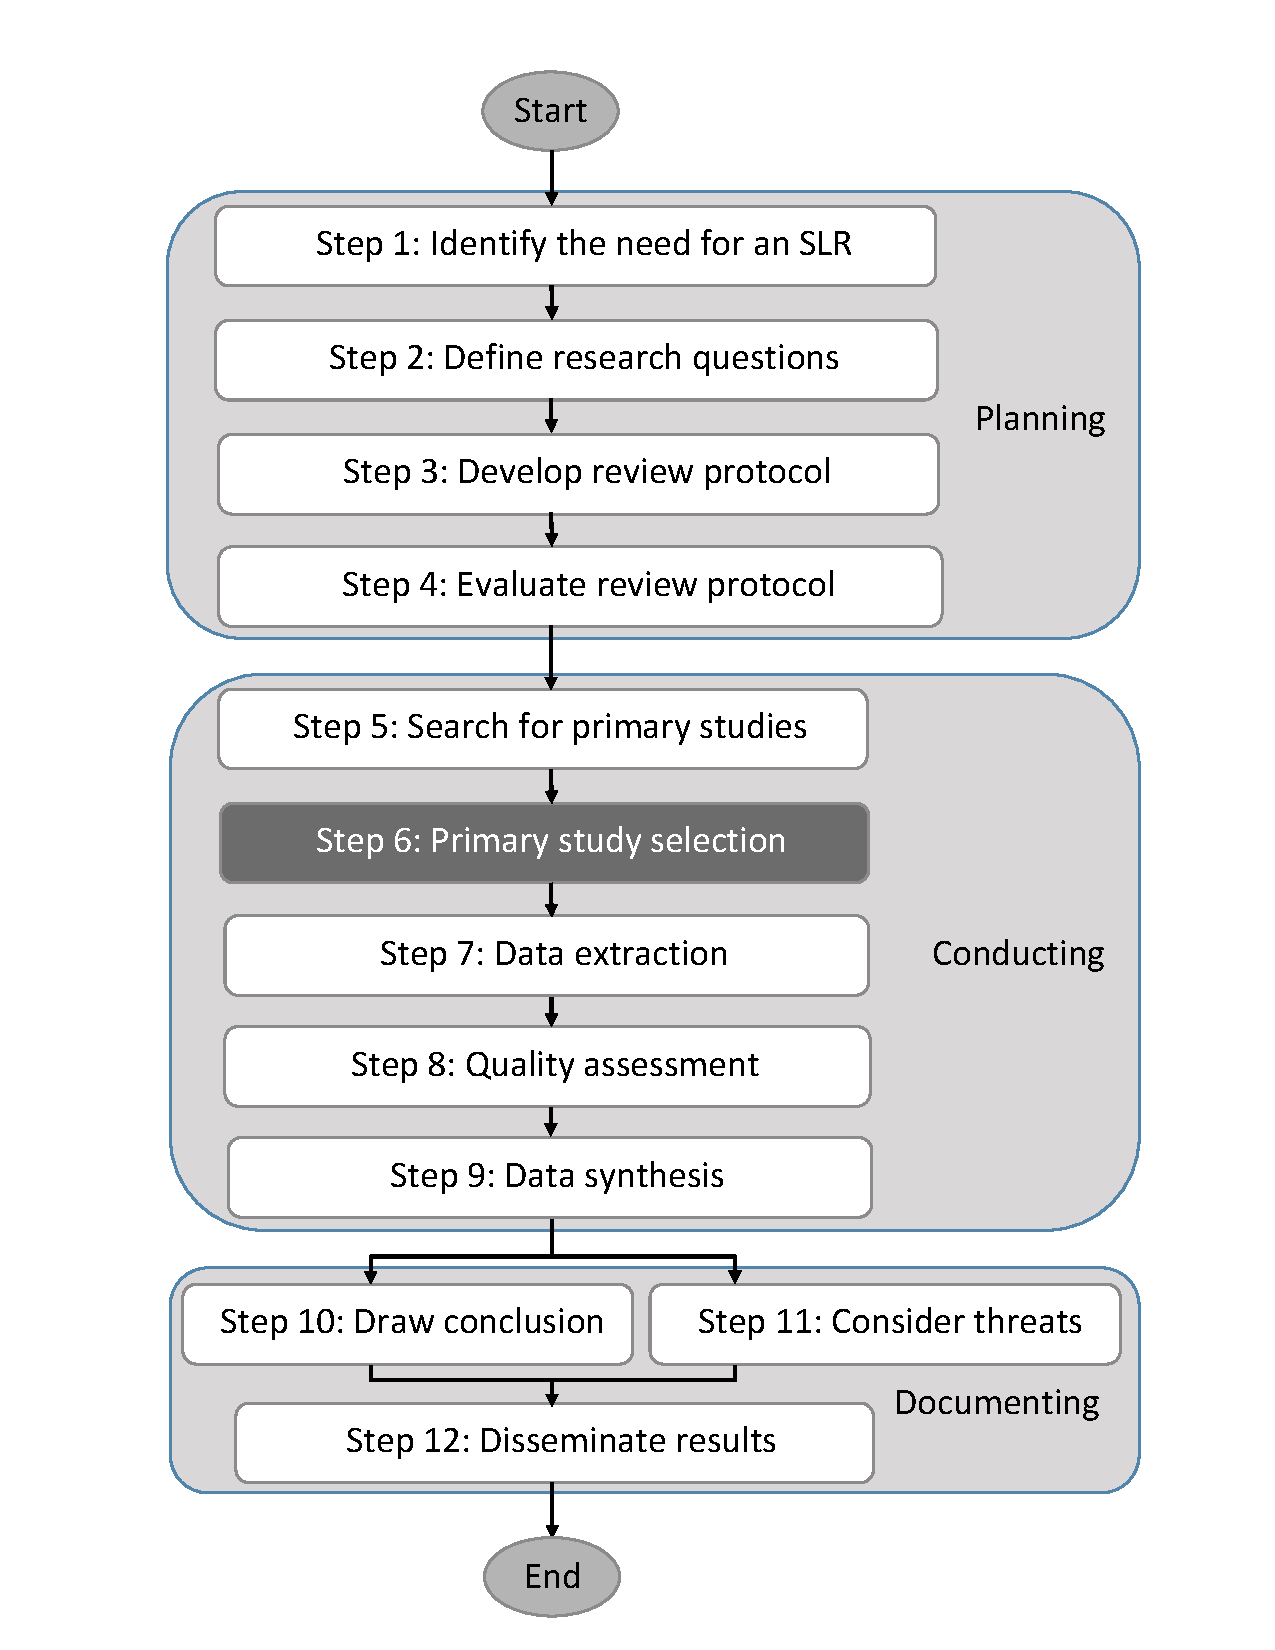
\includegraphics[width=\linewidth]{procedure.pdf}
    \caption{Systematic literature review steps suggested by~\cite{keele2007guidelines}. In this work, we focus on Step 6: primary study selection.}
    \label{fig: slr}
    \end{minipage}\quad
    \begin{minipage}[t]{.45\linewidth}
    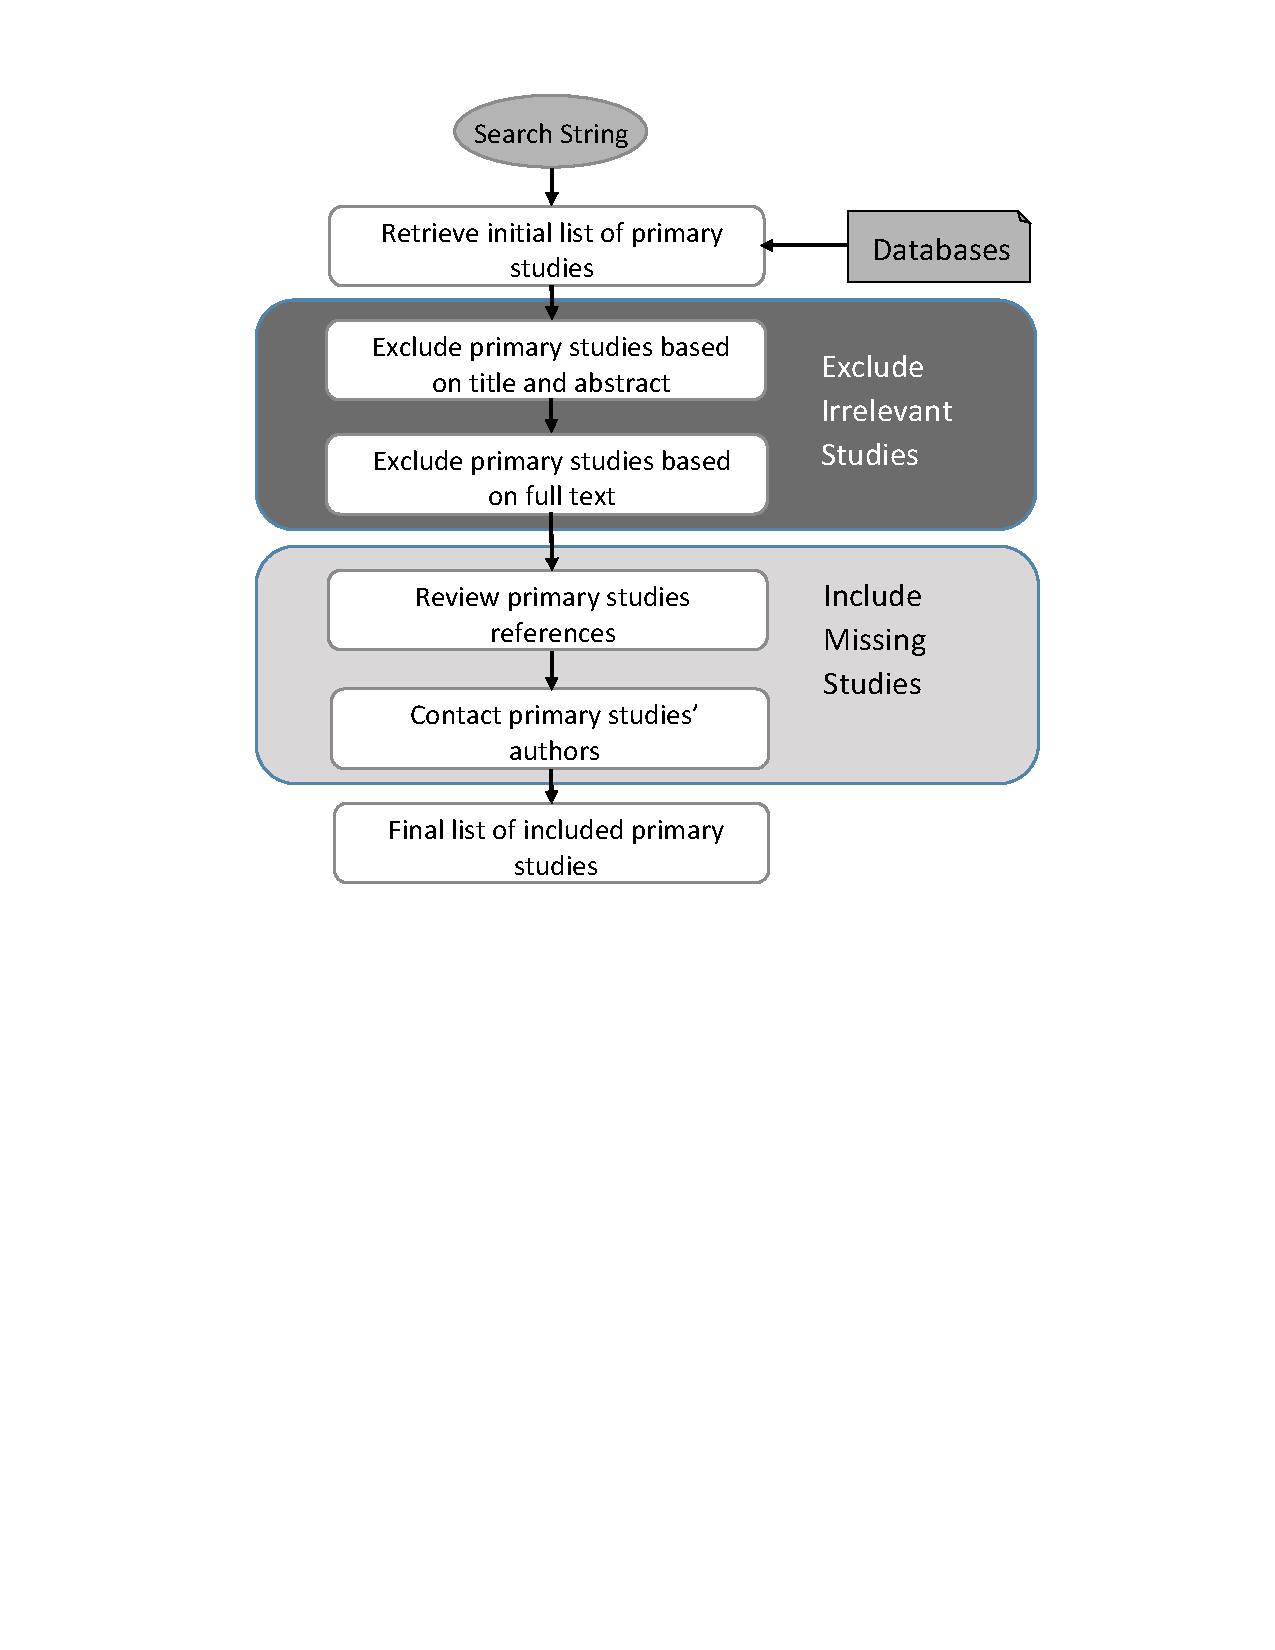
\includegraphics[width=\linewidth]{primary_study_selection.pdf}
    \caption{Primary study selection steps suggested by~\cite{keele2007guidelines}. In this work, we focus on the excluding irrelevant studies part.}
    \label{fig: prime}
    \end{minipage}
\end{figure}



% In contrast to a primary study, which investigates a specific research question,
% a systematic literature review is a form of secondary study aimed at
% identifying, evaluating and interpreting all available research relevant to a
% particular research question, topic area, or phenomenon of
% interest~\cite{keele2007guidelines}.
In the modern academic world, it is
impossible to start research without first knowing what other researchers have
done in the topic area. Conducting an SLR is one way to gain
background knowledge on a certain topic area.
If that SLR is published, then that paper becomes a useful research tool
for other researchers.  Kitchenham recommend SLRs to be standard
procedure in SE research~\cite{kitchenham2004evidence,keele2007guidelines}.

An SLR is usually conducted following the procedures in Fig.~\ref{fig: slr}. There can be variances on the real
implementations~\cite{wahono2015systematic,malhotra2015systematic,radjenovic2013software,unterkalmsteiner2012evaluation,hall2012systematic},
but all are based on the same guideline~\cite{keele2007guidelines}. Among all these steps, primary study selection is an important early step in SLRs. It starts with an initial candidate collection of studies retrieved by searching. In the first round of that process,
the reviewers' job is to read the titles and abstracts of candidate studies and classify each as ``relevant'' or ``irrelevant''. After the first round of review, the reviewers read through the full text of the previously included studies and make further decision on whether it is actually ``relevant'' or not. The whole procedure is shown in Fig.~\ref{fig: prime}. Typically, reviewers need to identify a final list of dozens of primary studies
among the initial collection of thousands of candidates. In terms of actual
cost, Malheiros has documented in~\cite{malheiros2007visual} that it requires 3
hours for one reviewer to review 100 studies.  This implies that it is a month's
work for one graduate student to review 3000 studies or three months' work to
review 9000 studies. 

In this work, we try to reduce the cost of the primary study selection by applying machine learning techniques to assist excluding irrelevant studies. In our {\em active learning} approach, each time a human reviews a paper, a learner updates its knowledge about what kind of documents are relevant. After that, the human uses that learned knowledge to guide the selection of the next paper to read.

The review cost of primary study selection can not be simply measured by the number of studies reviewed since the effort required for content review ($C_D$) is much higher than that for abstract review ($C_A$). Suppose one review process first identified $N_A$ ``relevant'' studies via reviewing $N$ abstracts, then reviewed the content of the $N_A$ studies and found $N_D$ of them are ``content relevant''. That is, to retrieve the $N_D$ ``content relevant'' studies, a total review cost of $C=N\times C_A+N_A\times C_D$ is required. To calculate this review cost, two level of relevance information is required (labels for ``abstract relevant'' and labels for ``content relevant''). However, most datasets of systematic literature review (including three datasets used in this study) have only one level of relevance information. As a result, only $N$ is used for review cost estimation since $N_A$ is not available. While this could be a fair metrics for comparing different treatments (smaller $N$ reflects less review cost in general), it is not a good estimation for how much effort saved by the text mining technique. Fortunately, the Kitchenham dataset provides two level of relevance information and we will explore the detailed review cost on this dataset in RQ3.





\subsection{Semi-Automated Tools for Literature  Reviews}

\subsubsection{Software Engineering Tools}

In recent years, various tools have been developed to facilitate SLRs in software engineering community, as summarized in~\cite{marshall2015tools,marshall2014tools,marshall2013tools}. These tools aim at providing support for protocol development~\cite{Molleri:2015:SWA:2745802.2745825,fernandez2010slr,hernandes2012using}, automated search~\cite{Molleri:2015:SWA:2745802.2745825,hernandes2012using}, primary study selection~\cite{Molleri:2015:SWA:2745802.2745825,hernandes2012using,fernandez2010slr,bowes2012slurp}, quality assessment~\cite{fernandez2010slr,bowes2012slurp,Molleri:2015:SWA:2745802.2745825}, data extraction and validation~\cite{Molleri:2015:SWA:2745802.2745825,hernandes2012using,fernandez2010slr,bowes2012slurp}, data synthesis~\cite{Molleri:2015:SWA:2745802.2745825,hernandes2012using,fernandez2010slr,bowes2012slurp},
and report write up~\cite{Molleri:2015:SWA:2745802.2745825,hernandes2012using,fernandez2010slr,bowes2012slurp}. It is extremely helpful to have a tool for managing the whole SLR process. However, the support for primary study selection using these tools is limited (e.g., to tasks such as assigning review jobs to multiple reviewers or to resolving disagreements).
Hence, we assert that the current SE SLR literature provides
no tool that can offer reductions in the effort required for primary study selection comparable to those reductions offered by active learning. Note that existing tools from Evidence-based Medicine offer active learning support and will be discussed in Section~\ref{sect: Evidence-based Medicine}.

Visual text mining (VTM) is a technique especially explored in Software Engineering community to support SLR. It is an unsupervised learning method which visualizes the relationship between candidate studies and helps the reviewer to make quick decisions. Malheiros et al.~\cite{malheiros2007visual} first applied VTM to support primary study selection in SLR. In their small-scale experiment (100 candidate studies, 31 of which are ``relevant''), VTM retrieves around 90\% of the ``relevant'' studies by spending about 30\% as much time as manual review. However, VTM requires some prior experience and knowledge of text mining and visualization techniques to use~\cite{bowes2012slurp}, and more case studies with large scale are needed to validate their results. 


Snowballing is another technique attracting much attention in SE SLR research. Given the inherent relevance relationship between a study and its citations, it is of high probability for the citations of (used in backward snowballing) and the studies cite (used in forward snowballing) a known ``relevant'' study to also be ``relevant''~\cite{kitchenham2004evidence}. Jalali and Wohlin~\cite{jalali2012systematic,wohlin2014guidelines} applied backward snowballing to search for primary studies in SE SLRs and found comparably good result as database search. Felizardo et al.~\cite{felizardo2016using} and Wohlin~\cite{wohlin2016second} applied forward snowballing to update SE SLRs and greatly reduced the number studies need to be reviewed comparing to a database search. This paper does not use snowballing since, as mentioned by Wohlin~\cite{wohlin2014guidelines}, snowballing starts with an initial set of relevant papers.
FASTREAD's task is very different: we start with zero relevant papers.



\subsubsection{Legal Electronic Discovery Tools}
\label{sect: Electronic Discovery}

Electronic Discovery (e-discovery) is a part of civil litigation where one party (the producing party), offers up materials which are pertinent to a legal case~\cite{krishna2016bigse}. This involves a review task where the producing party need to retrieve every ``relevant'' document in their possession and turn them over to the requesting party. It is extremely important to reduce the review cost in e-discovery since in a common case, the producing party will need to retrieve thousands of ``relevant'' documents among millions of candidates. Technology-assisted review (TAR) is the technique to facilitate the review process. The objective of TAR is to find as many
of the ``relevant'' documents in a collection as possible, with reasonable cost~\cite{grossman2013}. Various machine learning algorithms have been studied in TAR. So far, in every controlled studies, continuous active learning has outperformed others~\cite{cormack2014evaluation,cormack2015autonomy}, which makes it the state-of-the-art method in legal electronic discovery. It has also been selected as a baseline method in the total recall track of TREC 2015~\cite{roegiest2015trec}. Details on continuous active learning will be provided in Section~\ref{sect: Continuous Active Learning}. 

% Interestingly, the relationship between e-discovery and evidence-based medicine have been discussed in~\cite{leasesystematic} but their methods are still diverged. Relying on Grossman and Cormack~\cite{grossman2013} for support, many legal service providers have adopted TAR to facilitate the review process.

% In summary: the state-of-the-art active learning techniques are patient active learning in evidence-based medicine and continuous active learning in e-discovery.

\subsubsection{Evidence-based Medicine Tools}
\label{sect: Evidence-based Medicine}

Systematic literature reviews were first adopted from evidence-based medicine in
2004~\cite{kitchenham2004evidence}. To facilitate citation screening (primary
study selection) in systematic review, many groups of researchers have investigated different types of machine learning algorithms and evaluation mechanisms~\cite{o2015using,paynter2016epc}. 

Cohen et al. first applied text mining techniques to support citation screening and developed several performance metrics (including WSS) for assessing the performance of different techniques in 2006~\cite{cohen2006reducing}. While the great contribution of introducing machine learning and text mining into citation screening as well as the proposed performance metrics of Cohen has been widely acknowledged~\cite{o2015using}, most of Cohen's work focused on supervised learning which does not utilize unlabeled data and relies on random sampling to obtain the sufficiently large training set~\cite{cohen2006reducing,cohen2006effective,cohen2010prospective,cohen2011performance}.

Wallace et al. conducted a series of studies
with machine learning techniques, especially active
learning~\cite{wallace2010semi,wallace2010active,wallace2011should,wallace2012deploying,wallace2013active,wallace2013modernizing,nguyen2015combining}. Wallace
first set up a baseline approach called ``patient active learning'' (PAL), which will be explained later in this subsection, for machine learning assisted citation screening~\cite{wallace2010semi}. The performance of patient active learning is good enough (nearly 100\% of the ``relevant''
citations can be retrieved at half of the conventional review cost) to convince
systematic review conductors to adopt machine learning assisted citation
screening. Instead of improving this baseline method, Wallace then focused on other aspects of machine learning assisted citation screening such as introducing external expert knowledge~\cite{wallace2010active}, allocating review tasks to multiple experts~\cite{wallace2011should} or to crowdsourcing workers~\cite{nguyen2015combining}, and building a tool called abstrackr to provide overall support~\cite{wallace2012deploying}. Wallace's work on this topic is of exemplary high-impact and his core algorithm   (on simple expert screening),   is one of the most popular active learning techniques we have found in the evidence-based medical literature. That said, this technique has not been updated since 2010~\cite{wallace2010semi}. In this paper we are focused on the core active learning algorithm for cost minimization. Hence, we do not explore techniques such as Wallace's use of multiple experts (but in future work, we will explore this approach).

More recent work of Miva et al. explored alternative data balancing and query strategy in 2014~\cite{miwa2014reducing} and proposed a new treatment of Certainty plus Weighting. Instead of uncertainty sampling in PAL (and most conventional active learning approaches), Miva found that certainty sampling provides better results in clinical citation screening tasks. Similar conclusion for data balancing method as weighting relevant examples was found to be more effective than aggressive undersampling. Although not stated explicitly, Certainty plus Weighting keeps training until all ``relevant'' studies have been discovered, which differs from the stopping criteria of PAL. Aside from the core algorithm, additional views from latent Dirichlet allocation (LDA) has been found to be potentially useful.

Other work related to machine learning assisted citation screening do not
utilize active learning and active learning. Pure supervised learning requires a sufficiently large training set, which leads to a huge review cost~\cite{cohen2006reducing,adeva2014automatic}. Semi-supervised learning~\cite{liu2016comparative} does not utilize the human reviewers' feedback for updating the model, which leads to a depreciated performance in a long run. As a result, the patient active
learning proposed by Wallace et al.~\cite{wallace2010semi} and the Certainty plus Weighting approach by Miwa et al.~\cite{miwa2014reducing} are still considered to be the state-of-the-art method for citation screening in the scenario with no external knowledge and equally expensive reviewers. Details on these two approaches will be provided in Section~\ref{sect: Patient Active Learning} and \ref{sect: Certainty plus Weighting}.

There are also existing tools to support study selection in systematic reviews, e.g. Abstrakr\footnote{http://abstrackr.cebm.brown.edu}~\cite{wallace2012deploying}, EPPI-Reviewer\footnote{http://eppi.ioe.ac.uk/cms/er4/}~\cite{thomas2010eppi}, Rayaan\footnote{http://rayyan.qcri.org/}~\cite{Ouzzani2016}. Amazing features can be found in these tools such as a) Rayaan and EPPI-Reviewer: incorporated keyword search in screening; b) Rayaan and EPPI-Reviewer: deduplication; c) Rayaan and EPPI-Reviewer: define inclusion/exclusion criteria by terms; d) Abstrakr: user defined tags; e) all three: assign review tasks to multiple reviewers; f) all three: automatically extract data from PubMed. However, the active learning parts alone in these tools are depreciated. Under the condition that no additional feature (search, tags, define inclusion/exclusion terms) is used, we tried all three tools with one of our dataset-- Hall set (106 relevant in 8911 studies) and after reviewing 1000 studies, only 10 to 15 relevant ones were found, which was very close to a random sampling result without any learning. Since none of these tools are open-source, we cannot tell whether active learning is applied or how/when it is applied in each tool. This motivates us to develop an open source tool which focuses on active learning to support the primary study selection process. Details about our tool will be presented in Section~\ref{sect: tool}.



\section{Technical Notes}
\label{sect: Technical Briefing}

\begin{figure}[!t]
    \centering
    \subfloat[SVM without data balancing]
    {
        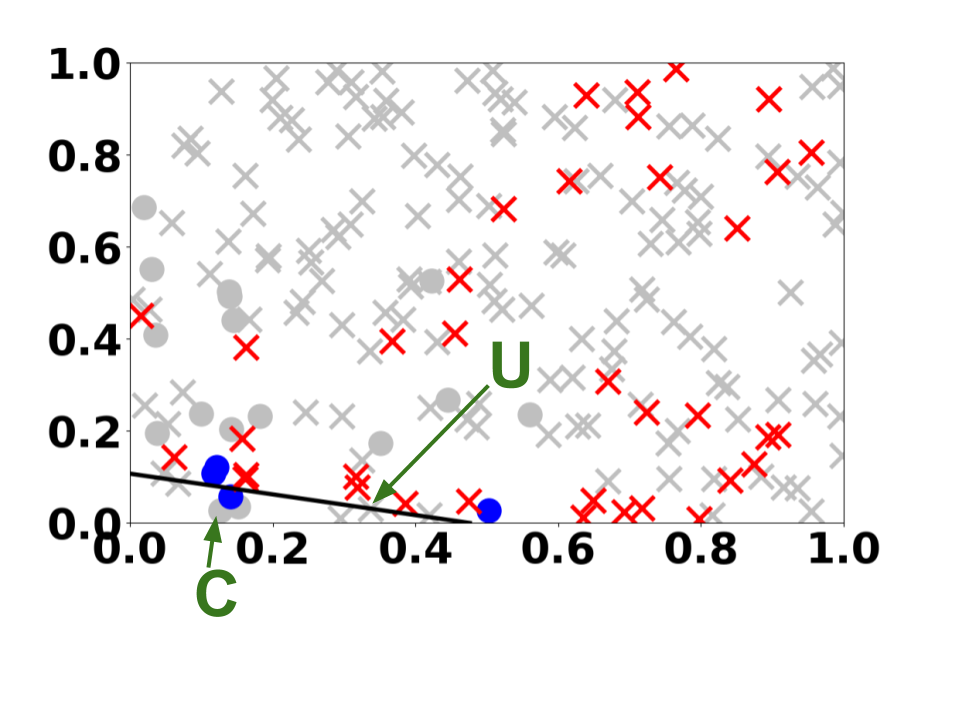
\includegraphics[width=0.3\linewidth]{simu22.png}
        \label{fig:train}
    }
    \subfloat[SVM with aggressive undersampling]
    {
        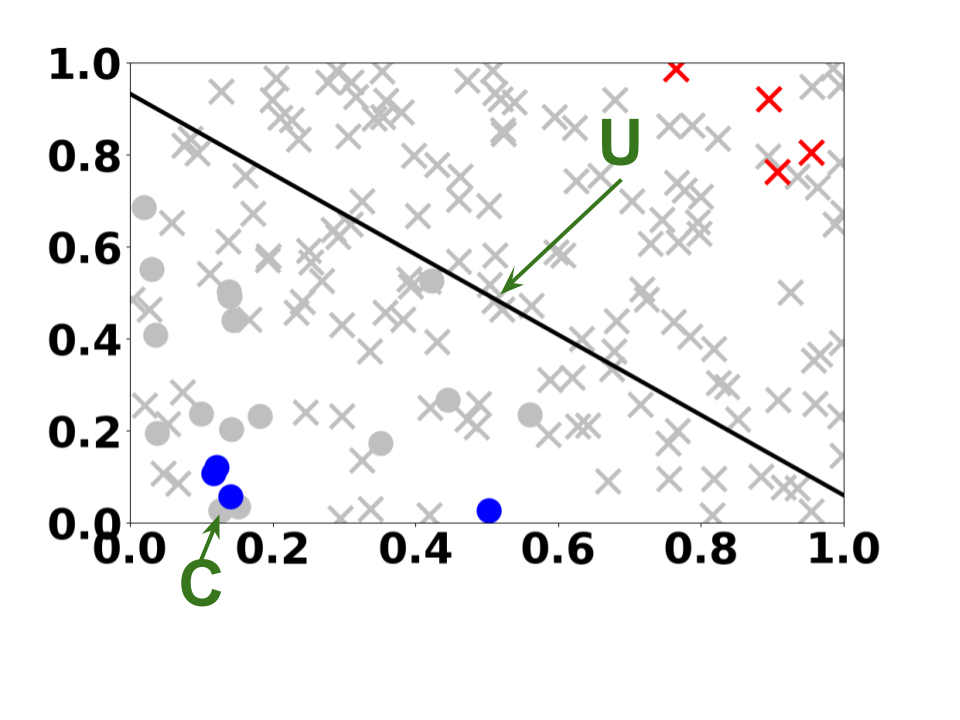
\includegraphics[width=0.3\linewidth]{simu23.png}
        \label{fig:train_a}
    }
    \subfloat[SVM with Weighting]
    {
        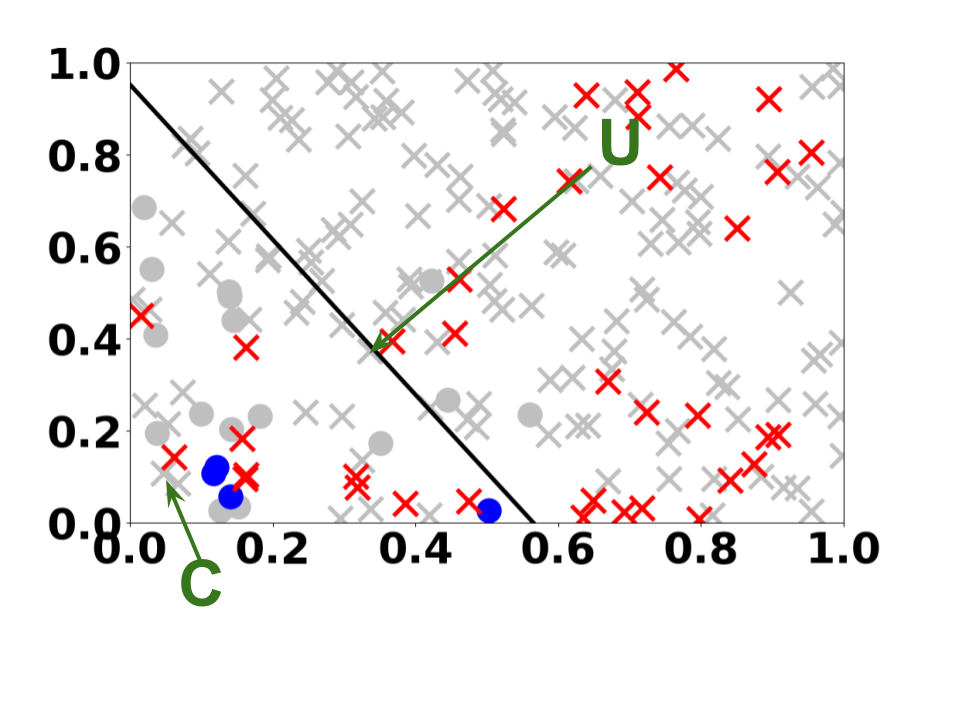
\includegraphics[width=0.3\linewidth]{simu24.png}
        \label{fig:test}
    }

    \caption{A demonstration of how SVM model is trained on imbalanced data, where ``$O$'' is the minority class, ``relevant'' studies in SLR, ``$X$'' is the majority class, ``irrelevant'' studies in SLR, markers in gray are the unlabeled studies, and black line is SVM decision plane. In (b), aggressive undersampling balances the training data by throwing away majority class examples closest to the old decision plane in (a). In (c) Weighting balances the training data by putting more weight on the minority class examples. Uncertainty sampling returns the unlabeled examples closest to the decision plane while certainty sampling returns the unlabeled examples furthest to the decision plane from the bottom-left side.}
    \label{fig:SVM}
\end{figure}

In this section, we provide details on technical terms 
used in the paper,  along with some brief introductory
notes on machine learning techniques used in this study.


\subsection{Linear Review}
\label{sect: Linear Review}

Linear review lets the reviewer to review and label every candidate study in a random order. This is still the most popular review method when there is unlimited review budget and completeness is the major objective. In this study, linear review works as a baseline method where no text mining technique is applied.

\subsection{Support Vector Machine}
\label{sect: Support Vector Machine}

Support vector machines (SVM) are a well-known and widely used classification method. The idea behind is to map input data to a high-dimension feature space and then construct a linear decision plane in that feature space~\cite{cortes1995support}. Linear SVM~\cite{joachims2006training} has been proved to be a useful model in SE text mining~\cite{krishna2016bigse} and is applied in the state-of-the-art active learning methods of both evidence-based medicine and electronic discovery~\cite{miwa2014reducing,wallace2010semi,cormack2014evaluation}. Fig.~\ref{fig:SVM} illustrates how linear SVM model is trained on a two-dimension feature space with different data balancing techniques.

\subsection{Active Learning}
\label{sect: Active learning}

Active learning is a cost-aware machine learning algorithm where labels of training data can be acquired with certain costs. The key idea behind active learning is that a machine learning algorithm can perform better with less
training if it is allowed to choose the data from which it learns~\cite{settles2012active}. There are several scenarios active learning is applied to, such as membership query synthesis, stream-based selective sampling, and pool-based sampling~\cite{settles2010active}. There are also different query strategies of active learning, such as uncertainty sampling, query-by-committee, expected model change, expected error reduction, variance reduction, and density-weighted methods~\cite{settles2010active}. Here, we will briefly introduce one scenario and two query strategies, which will be used in our later experiments and discussions.

\textbf{Pool-based sampling} is the scenario of primary study selection. This scenario starts with a fixed size pool of unlabeled data. Labels for the data can be acquired by querying an oracle selectively. The goal of pool-based sampling is to select the most informative data in the pool for query, thereby building a better model with less training.

\textbf{Uncertainty sampling} is the query strategy utilized in the state-of-the-art active learning technique of evidence-based medicine~\cite{wallace2010semi,wallace2010active}. It is also recognized as the most simple and commonly used query strategy~\cite{settles2010active}. In this query strategy, uncertainty sampling queries the instances about which the learner is least certain how to label. These instances are those (a) whose posterior probability of being positive are nearest 0.5 in probabilistic models or (b) closest to the decision boundary in models such as SVM. 

\textbf{Certainty sampling} is another query strategy which is applied in the state-of-the-art active learning technique of electronic discovery~\cite{cormack2014evaluation,cormack2015autonomy} and is also preferred over uncertainty sampling by Miwa et al. \cite{miwa2014reducing}. In contrast to uncertainty sampling, certainty sampling queries the instances about which the learner is most certain to label as positive. These instances are those (a) whose posterior probability of being positive are highest in probabilistic models, or (b) lies in the positive side of the decision boundary and furthest to the decision boundary in models such as SVM. This query strategy is usually NOT used when building the classifier of active learning since it is commonly believed that examples queried by certainty sampling contains less information than those by uncertainty sampling.

% \subsection{active Learning}
% \label{sect: active Learning}

% active learning is a combination of human decisions and machine
% suggestions~\cite{tredennick2015}. In this approach:
% \begin{itemize}
% \item
% Humans read a stream of documents, commenting on whether or
% not each one is ``relevant''.
% \item
%   Machine learners use feedback from the human opinion to
%   incrementally update their models actively.
% \item
%   The models generated via machine learning are used
%   to sort the stream of documents such that the humans focus on the
%   most informative documents.
%   \end{itemize}

% This is a
% pool-based active learning scenario since \textbf{a)} the process starts with a fixed size candidate list without any labels and \textbf{b)} training examples gradually become available to the learner as the human reviewer reviews the documents.  However, an important difference between active learning and other active learning methods is that every document labeled as ``relevant'' has been reviewed by a human. The machine never makes the final decision on whether a document is ``relevant''; a human makes such decisions and the machine only suggests a review order based on the human input. As a result, instead of building a better classification model, the objective of active learning is to retrieve most ``relevant'' documents from a pool of candidates while manually reviewing as few documents as possible. 

% Simple active learning, which is pool-based active learning with uncertainty sampling~\cite{settles2012active}, is the most basic form of learning methods
% applied to active learning. Although simple active learning achieves
% satisfactory performance, it has been outperformed by the state-of-the-art active learning techniques in both evidence-based medicine~\cite{wallace2010semi} and electronic discovery~\cite{cormack2014evaluation}. 


\subsection{Patient Active Learning}
\label{sect: Patient Active Learning}

One of the state-of-the-art active learning method in evidence-based medicine, patient active learning (PAL) can be described as following~\cite{wallace2010semi}:

\begin{itemize}

\item
{\bf Stage I: Construct an initial seed training set} by randomly sampling from the candidate study pool and asking a human reviewer to label the sampled papers as ``relevant'' or ``irrelevant''. Stop and proceed to Stage II when \textit{enough} ``relevant'' studies have been retrieved to represent the ``relevant'' class. (Note that Wallace et al.~\cite{wallace2010semi} did not provide an explicit definition of \textit{``enough''}.)

\item
{\bf Stage II: Build the classifier}, which is a linear SVM, by repeatedly training on labeled studies and uncertainty sampling. Unlabeled studies in the pool will be ranked in the descending order of uncertainty (uncertainty sampling). The human reviewer labels the studies in the ranked order and feeds them back to retrain the classifier. Stop and proceed to Stage III when the classifier is \textit{stable}. (Note that Wallace et al.~\cite{wallace2010semi} did not provide an explicit definition of \textit{``stable''}.)

\item
{\bf Stage III: Prediction.} Retrain the classifier with \textbf{aggressive undersampling} and then stop training. Unlabeled studies in the pool will be ranked in the descending order of the classifier's prediction probability of being ``relevant'' (certainty sampling as discussed in Section~\ref{sect: Active learning}). The human reviewer labels the studies in the ranked order until finished (running out of review cost budget, enough ``relevant'' studies found, or no more ``relevant'' studies are detected in multiple rounds).

\end{itemize}

{\bf Aggressive undersampling: }The data for citation screening are (at times, extremely) imbalanced, i.e., the prevalence of ``relevant'' citations is always smaller than $50\%$ (and often much smaller). Classification algorithms are typically optimized for overall accuracy, rather than accuracy, precision, recall to a particular class. This becomes a problem when only the performance on a minority class matters. Patient active learning utilizes aggressive undersampling for data balancing. By throwing away majority (``irrelevant'') class training examples which are closest to the SVM decision hyperplane, it undersamples the majority class training examples to the same size as minority (``relevant'') class. It is a recall friendly undersampling method since the new decision hyperplane is pushed away from the minority class. An exampling of aggressive undersampling is shown in Fig.~\ref{fig:SVM}.

\subsection{Certainty plus Weighting}
\label{sect: Certainty plus Weighting}

Another state-of-the-art active learning method in evidence-based medicine, Miwa et al. suggested using certainty sampling and weighting instead of uncertainty sampling and aggressive undersampling in PAL. This method can be described as following~\cite{miwa2014reducing}:

\begin{itemize}

\item
{\bf Stage I: Construct an initial seed training set} by randomly sampling from the candidate study pool and asking a human reviewer to label the sampled papers as ``relevant'' or ``irrelevant''. Stop and proceed to Stage II when \textit{enough} ``relevant'' studies have been retrieved to represent the ``relevant'' class. (Same as PAL.)

\item
{\bf Stage II: Build the classifier}, which is a linear SVM, by repeatedly training on labeled studies with \textbf{Weighting} and certainty sampling. Unlabeled studies in the pool will be ranked in the classifier's prediction probability of being ``relevant''(certainty sampling). The human reviewer labels the studies in the ranked order and feeds them back to retrain the classifier. Training continues until finished (running out of review cost budget, enough ``relevant'' studies found, or no more ``relevant'' studies are detected in multiple rounds).

\end{itemize}

{\bf Weighting: }Weighting balances the training examples by putting more weights on the minority class. The weighting factor is calculated as \emph{Size of Majority Class Training Examples / Size of Minority Class Training Examples}. An exampling of Weighting is shown in Fig.~\ref{fig:SVM}.

Miwa et al. also suggested that clustering by LDA before review has the potential to provide better performance in certain situations. However, this study focuses on refactoring and comparing the core active learning methods, same preprocessing step (without LDA) is applied to every treatment. The exploration of different feature engineering and preprocessing are planned for future works.

\subsection{Continuous Active Learning}
\label{sect: Continuous Active Learning}

The state-of-the-art active learning method in e-discovery, continuous active learning (CAL) can be described as following~\cite{cormack2014evaluation,cormack2015autonomy,tredennick2015}:

\begin{itemize}

\item
{\bf Stage I: Construct an initial seed training set} by random sampling from the candidate study pool and ask a human reviewer for labels. Stop and proceed to Stage II as soon as \textbf{ONE} ``relevant'' study is retrieved.

\item
{\bf Stage II: Predict and retrain} by repeatedly training on labeled studies and certainty sampling. Unlabeled studies in the pool will be ranked in the descending order of the classifier's prediction probability of being ``relevant'' (certainty sampling). A human reviewer labels the studies in the ranked order and feeds them back to retrain the classifier until finished.

\end{itemize}

In contrast to PAL, CAL is the opposite of ``patient''. It starts to train the model as soon as \textit{ONE} ``relevant'' study shows up and skips the uncertainty sampling stage, which is believed to be essential for active learners~\cite{settles2012active}. Since the objective is to retrieve ``relevant'' studies with candidates reviewed as few as possible, it is reasonable not to waste any single effort on building up the classifier~\cite{cormack2014evaluation,tredennick2015}. Also, the experiment results in~\cite{cormack2014evaluation} has demonstrated the value of this ``greedy'' strategy.

Among all the three state-of-the-art treatments, CAL and PAL are different in every aspect while Certainty plus Weighting is in the middle of these two and supports a different data balancing method.


\section{Methods}
\label{sect: Method}

This section describes our datasets and their preparation then describes and refactors state-of-the-art methods for active learning.
This refactoring process will create FASTREAD, our preferred active learning
method. 

\subsection{Datasets}
\label{sect: datasets}

Although a large number of SLRs are published every year, there is no dataset clearly documenting the details in primary study selection. As a result, three datasets are created based on the information in existing SLRs and being used in this study to simulate the process of excluding irrelevant studies. The three datasets are named after the authors of their original publication source-- Wahono dataset from Wahono et al. 2015~\cite{wahono2015systematic}, Hall dataset from Hall et al. 2012~\cite{hall2012systematic}, and Radjenovi{\'c} dataset from Radjenovi{\'c} et al. 2013~\cite{radjenovic2013software}. 

For each of the datasets, the search string \textbf{S} and the final inclusion list \textbf{I} from the original publication are used for the data collection. We retrieve the initial candidate collection \textbf{C} from IEEE Xplore with the search string (slightly modified to meet the requirement of IEEE Xplore). Then make a final list of inclusion \textbf{R} as \textbf{R} = \textbf{I} $\cap$ \textbf{C}. Here, for simplicity reason we only extract candidate studies from IEEE Xplore. We will explore possibilities for efficiently utilizing multiple data sources in the future work but in this paper, without loss of generality, we only extract initial candidate list from single data source. In this way, we created three datasets that reasonably resemble real SLR selection results assuming that any study outside the final inclusion list \textbf{I} is irrelevant to the original SLRs. A summary of the created datasets is presented in Table~\ref{tab: number}.

Apart from the three created datasets, one dataset (Kitchenham) is provided directly by the author of Kitchenham et al. 2010~\cite{kitchenham2010systematic} and includes two levels of relevance information. In general, only the ``content relevant'' labels are used in experiments for a fair comparison with other datasets. Additionally, the ``abstract relevant'' labels are used for detailed review cost analysis in RQ3. Summary of Kitchenham dataset is also presented in Table~\ref{tab: number}.

All the above datasets are available on-line at {\em https://doi.org/10.5281/zenodo.837298}.

\begin{table}
\caption{Descriptive statistics for experimental datasets}
\label{tab: number}
\begin{center}
\begin{tabular}{ |l|c|c|c|c| }
  \hline
   Datasets & \multicolumn{2}{|c|}{Generated} & \multicolumn{2}{|c|}{Original} \\
  \cline{2-5}
  & \#Candidate $|$\textbf{C}$|$ & \#Relevant $|$\textbf{R}$|$& \#Candidate & \#Relevant $|$\textbf{I}$|$\\
  \hline
  Wahono & 7002 & 62 & 2117 & 72\\
  \hline
  Hall & 8911 & 106 & 2073 & 136 \\
  \hline
  Radjenovi{\'c} & 6000 & 48 & 13126 & 106\\
  \hline
  Kitchenham & 1704 & 44 (132) & 1704 & 44 (132) \\
  \hline
\end{tabular}
\end{center}
{\footnotesize Our datasets are generated using information in the original SLR literature. Our candidate studies are retrieved by applying similar if not the same the search string from original SLR literature and search in IEEE Xplore. The set of our relevant studies is the intersection of the set of our candidate studies and the set of final included studies in the original SLR literature. Kitchenham dataset is different as it is provided directly by Kitchenham and it has two level of relevance labels-- 132 relevant studies by title and abstract review and within which, 44 relevant studies by content review.}
\end{table}




\begin{figure}[t]
    \centering
    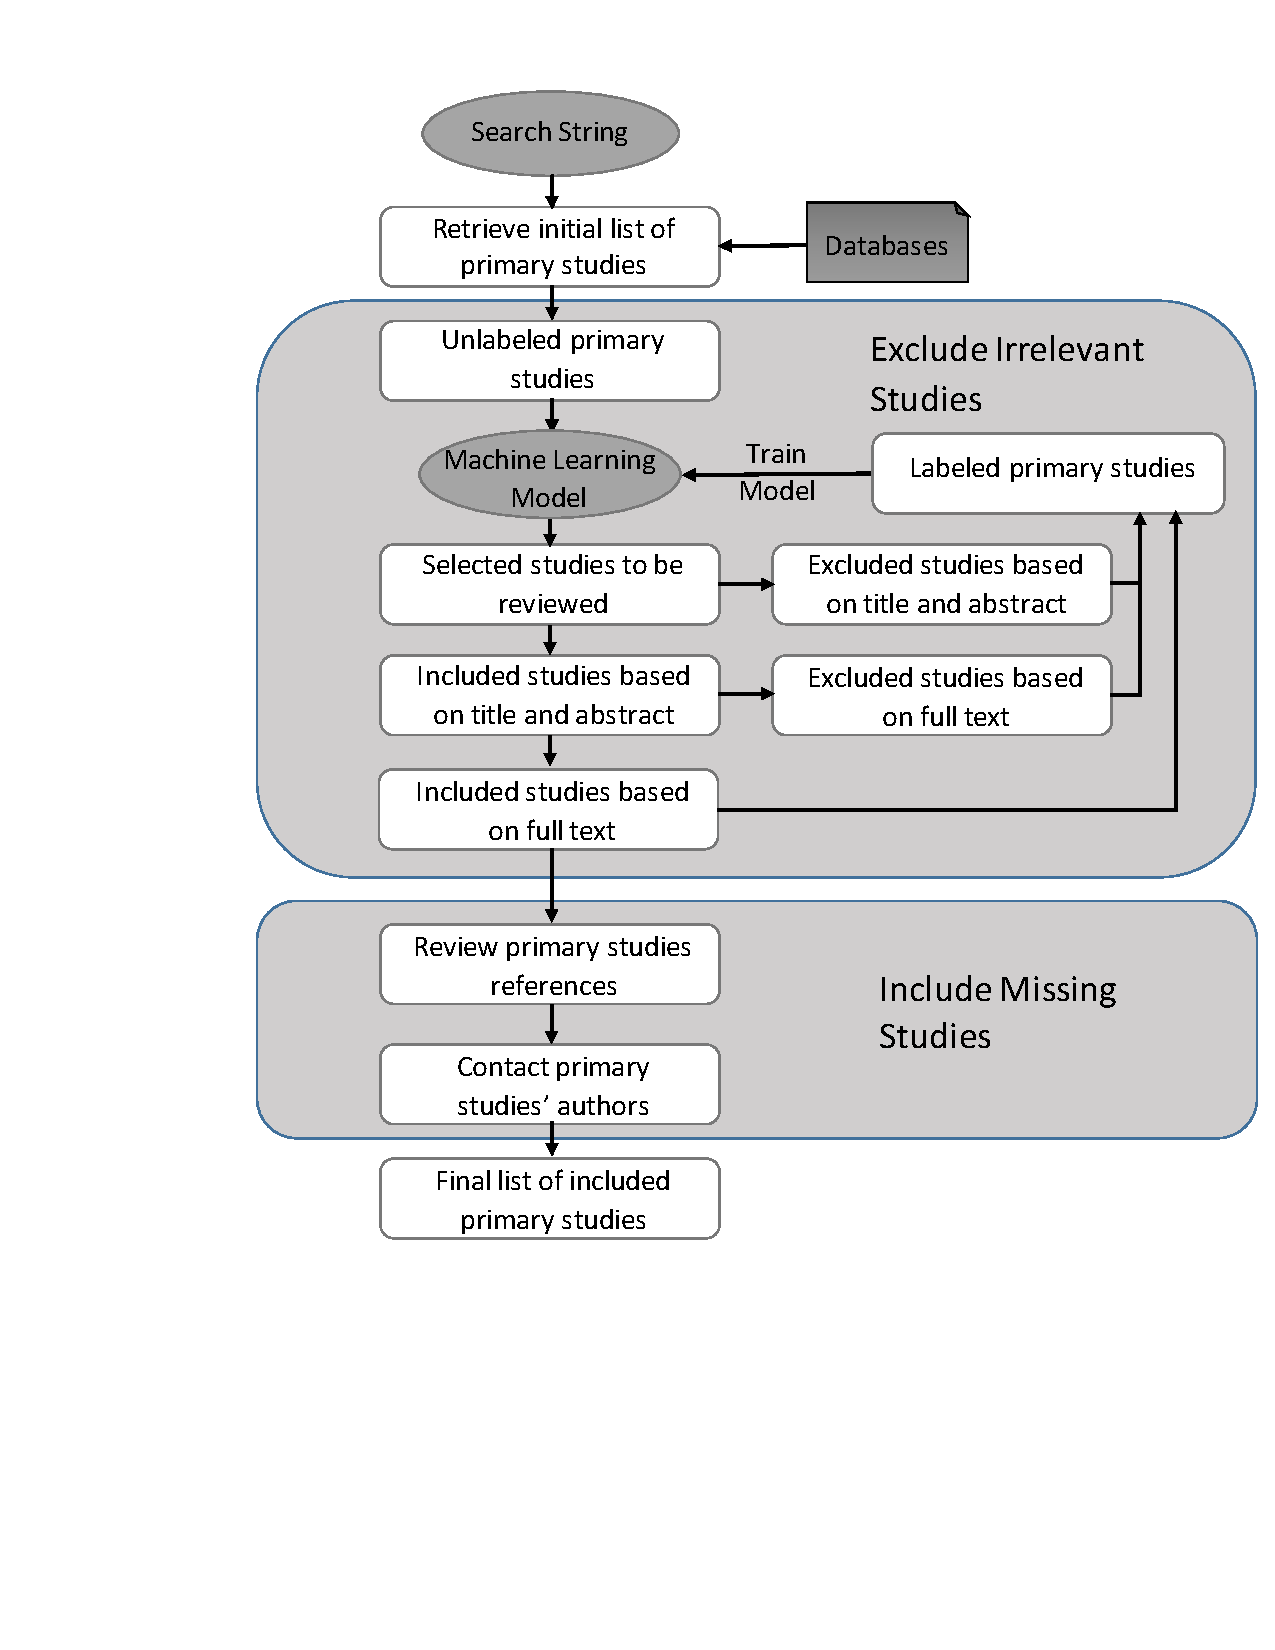
\includegraphics[width=0.6\linewidth]{Learning_based_primary_study_selection.pdf}
    \caption{Human-in-the-loop Primary study selection.}
    \label{fig: learning}
\end{figure}

\subsection{Human-in-the-loop Primary Study Selection}
\label{subsect: Learning based Primary Study Selection}


In contrast to the classical primary study procedures in Fig.~\ref{fig: prime}, with active learning as part of the process, the general form of human-in-the-loop primary study selection is presented in
Fig.~\ref{fig: learning}. Reviewers first review the title and abstract of the
suggested study, determine whether it is ``abstract relevant'' or ``abstract irrelevant''. If the study is relevant by title and abstract, the reviewer will then read the full text of the study and make the final decision-- ``content relevant'' or ``content irrelevant''. In the meantime, all the reviewed
studies will go into the training set. Note that only the title and abstract of the training set studies will be used to train the active learning model, thus making data extraction for training examples easy. Note that in this process, two-level relevance labels are generated and should be available to the active learning model. However, the fact is, for most of our datasets, ``abstract relevant'' labels are missing since they are not reported in the original SLR literature. As a result, only ``content relevant'' labels are being used for training in our experiments. In the rest of the paper, when we say ``relevant'', it means ``content relevant'' while ``irrelevant'' studies include every study that is not ``content relevant'' (``abstract relevant'' but ``content irrelevant'' or ``abstract irrelevant'').

The objective of Human-in-the-loop primary study selection (or machine learning
assisted citation screening or TAR) is different from that of common active
learning scenarios. Instead of trying to build a classifier as good as possible,
human-in-the-loop primary study selection seeks methods to retrieve most
``relevant'' studies with candidate studies reviewed as few as possible. This
difference in the objective leads to a different performance metrics (further explained in Section~\ref{subsect: Performance Metrics}) and thus
makes conventional active learning methods being outperformed by specially
designed methods like PAL~\cite{wallace2010semi}, Certainty plus Weighting~\cite{miwa2014reducing} in evidence-based
medicine and CAL~\cite{cormack2014evaluation,cormack2015autonomy} in
e-discovery.



\subsection{Algorithm Code}
\label{sect: Algorithm Code}

Differences of the three state-of-the-art active learning techniques for systematic reviews are from four aspects: 1) when to start training; 2) query strategy; 3) whether to stop training; 4) data balancing.

\begin{itemize}

\item
{\bf When to start training}: 

\textbf{P} stands for ``patient''. As suggested by Wallace et al.~\cite{wallace2010semi}, ``hasty generation'', which means start training with too few relevant examples, may leads to deteriorate performance. The algorithm keeps random sampling until a sufficient number of ``relevant'' studies retrieved. In our experiments, the sufficient number of ``relevant'' studies retrieved is set to $5$, which means when at least $5$ ``relevant'' studies have been retrieved by random sampling, the algorithm goes into next stage. PAL~\cite{wallace2010semi} and Certainty plus Weighting~\cite{miwa2014reducing} use \textbf{$P$} for when to start training.

\textbf{H} is the opposite. The algorithm stops random sampling as long as {\em ONE} ``relevant'' studies are retrieved, as suggested in CAL~\cite{cormack2014evaluation,cormack2015autonomy}.

\item
{\bf Query strategy}: 

\textbf{U} stands for ``uncertainty sampling''. The algorithm utilizes
uncertainty sampling to build the classifier, where unlabeled examples closest to the SVM decision plane are sampled for query. PAL~\cite{wallace2010semi} uses \textbf{U} for Query strategy.

\textbf{C} stands for ``certainty sampling''. The algorithm utilizes certainty sampling to build the classifier, where unlabeled examples furthest to the SVM decision plane and lie in the ``relevant'' side are sampled for query. Certainty plus Weighting~\cite{miwa2014reducing} and CAL~\cite{cormack2014evaluation,cormack2015autonomy} use \textbf{C} for query strategy.

\item
{\bf Whether to stop training}: 

\textbf{S} stands for ``stop training''. The algorithm stops training
once the classifier is stable. In our experiments, the classifier is treated as stable once more than $30$ ``relevant'' studies have been retrieved as training examples. PAL~\cite{wallace2010semi} uses \textbf{$S$} for whether to stop training.

\textbf{T} stands for ``continue training''. The algorithm never stops
training as suggested in CAL~\cite{cormack2014evaluation,cormack2015autonomy} and Certainty plus Weighting~\cite{miwa2014reducing}. If query strategy is \textbf{U}, algorithm switches to certainty sampling after classifier is stable but training never stops.

\item
{\bf Data balancing}: 

\textbf{N} stands for ``no data balancing''. The algorithm does not balance the training data as suggested by CAL~\cite{cormack2014evaluation,cormack2015autonomy}.

\textbf{A} stands for ``aggressive undersampling''. The algorithm utilizes aggressive undersampling when classifier is stable, as suggested by PAL~\cite{wallace2010semi}.

\textbf{W} stands for ``Weighting''. The algorithm utilizes Weighting for data balancing (before and after the classifier is stable), as suggested by Certainty plus Weighting~\cite{miwa2014reducing}.

\textbf{M} stands for ``mixing of Weighting and aggressive undersampling''. Weighting is applied before the classifier is stable while aggressive undersampling is applied after the classifier is stable. This treatment comes from the observation that ``Weighting'' performs good in early stages while ``aggressive undersampling'' performs good in late stages.

\end{itemize}
As a result, we ended up with 32 treatments including the state-of-the-art treatments as
\begin{itemize}
\item
\textbf{PUSA}: patient active learning~\cite{wallace2010semi,wallace2010active};
\item
\textbf{PCTW}: Certainty plus Weighting~\cite{miwa2014reducing};
\item
\textbf{HCTN}: continuous active learning~\cite{cormack2014evaluation,cormack2015autonomy}. 
\end{itemize}
All the 32 algorithms are tested and compared in Section~\ref{sect: Experiments}.

\section{Experiments}
\label{sect: Experiments}

This section describes the experimental procedures that we used to evaluate the treatments described in Section~\ref{sect: Algorithm Code} on the datasets described in Section~\ref{sect: datasets}. 

There is no human activity involved in these experiments, when asked for a label, the true label in the dataset is queried instead of a human reviewer. As a result, each experiment can be repeated with different random seed to capture variances and also makes reproducing the experiments possible. Each experiment is a simulation of one specific treatment on one dataset:

\begin{enumerate}
\item
Starts with an unlabeled collection of candidate studies, e.g. 8911 in Hall as shown in Table~\ref{tab: number}.

\item
\label{select}
Train a model on current labeled examples if enough labeled examples are available.

\item
Select $N=10$ studies based on the prediction of machine learning model on unlabeled examples for review. If no model is trained yet, random sample $N=10$ unlabeled studies.

\item
Query the true labels of the selected studies, i.e. 106 ``relevant'' and 8805 ``irrelevant'' in Hall as shown in Table~\ref{tab: number}, label them as their true labels.

\item
Go back to \ref{select} until finished.

\end{enumerate}


\subsection{Controlled Variables}
\label{subsect: Controlled Variables}

For the sake of a fair comparison, different treatments in Section~\ref{sect: Algorithm Code} share an identical set of controlled variables including preprocessing, featurization and classifier. 

\subsubsection{Preprocessing and Featurization}

Each candidate study in the initial list is first tokenized by stop words removal after concatenating its title and abstract. After tokenization, the bag of words are featurized into a term frequency vector. Then, reduce the dimensionality of the term frequency vector with to keep only $M=4000$ of the terms with highest tf-idf\footnote{For term $t$ in document $d$, $Tfidf(t, d)=w^t_d\times (\log \frac{|D|}{\sum_{d\in D} sgn(w^t_d)}+1)$ where $w^t_i$ is the term frequency of term $t$ in document $d$. For term $t$, $Tfidf(t) = \sum_{d\in D} Tfidf(t,d) = \sum_{d\in D} w^t_d \times (\log \frac{|D|}{\sum_{d\in D} sgn(w^t_d)}+1)$ and is used for feature selection.} score and normalize the hashed matrix by its L2 norm each row at last. TfidfVectorizer in scikit-learn is utilized for the above preprocessing and featurization steps. Alternatives such as stemming, LDA~\cite{blei2003latent}, paragraph vectors~\cite{le2014distributed} require exploration and are scheduled in our future works. 


\subsubsection{Classifier}

For this work we use a linear SVM as the classifier.
SVMs learn a hyperplane that separate relevant from irrelevant examples
in the training data. Linear SVMs do not make complicated assumptions about the data space and so are known to scale to very large, high-dimensional problems~\cite{joachims2006training}. Such linear SVMs are widely used in the state-of-the-art solutions~\cite{miwa2014reducing,cormack2015autonomy,wallace2010semi}. SVM's hyperplane is a natural tool for deciding what examples to show next to the human user. As discussed in Section~\ref{sect: Technical Briefing}, uncertainty sampling prefers the examples {\em closest} to the hyperplane boundary since these are the ones whose classification will
change, given small changes to the test data. On the other hand, certainty sampling prefers the examples with {\em highest} SVM predictions of being positive. SVC (set to be linear kernel) with default parameters in scikit-learn is utilized as the classifier.


\subsection{Performance Metrics}
\label{subsect: Performance Metrics}

Common active learning aims for building a better model with less training. Therefore, its performance metrics is usually some \textbf{accuracy, precision, recall} on the model prediction vs \textbf{training size} curve. The \textbf{accuracy, precision, recall} are measured on some validation set.

On the other hand, since the goal of human-in-the-loop primary study selection described in Section~\ref{subsect: Learning based Primary Study Selection} is different from that of common active learning, the performance metrics is also different. In human-in-the-loop primary study selection, the performance of each algorithm is evaluated by its \textbf{recall} vs. \textbf{studies reviewed} curve. The \textbf{recall} here is not a measurement on the trained model, but the number of ``relevant'' studies retrieved over the total number of ``relevant'' studies. An algorithm is better than the other if it can retrieve more ``relevant'' studies with fewer studies reviewed. This performance metrics is suggested by~\cite{cormack2015autonomy,cormack2014evaluation,tredennick2015} and best fits the objective of human-in-the-loop primary study selection. To enable a statistical analysis of the performances, the \textbf{recall} vs. \textbf{studies reviewed} curve is cut by a $0.95$ \textbf{recall} line and \textbf{studies reviewed} when reaching $0.95$ \textbf{recall} is used to assess performances. The reason behind $0.95$ \textbf{recall} is that a) $1.00$ \textbf{recall} can never be guaranteed by any text mining method unless all the candidate studies are reviewed; b) $0.95$ \textbf{recall} is usually considered acceptable in evidence-based medicine~\cite{cohen2011performance,cohen2006reducing,o2015using} despite the fact that there might still be ``relevant'' studies missing~\cite{shemilt2016use}. As a result, two numbers are recorded during experiments:
\begin{itemize}
\item
X95 = $\min \{x | r(x)\geq0.95 R\}$
\item
WSS@95 = $0.95-\text{X95}/T$
\end{itemize}
where in a total number of $T$ candidate studies, $R$ of them are ``relevant'' according to true labels, and $r(x)$ is the number of ``relevant'' studies found when $x$ studies have been reviewed.

Each treatment on each dataset is tested for 30 repeats\footnote{It is suggested that usually a sampling size of $30$ is adequate~\cite{isotalo2001basics}.} with random seeds ranging from 0 to 29. The 30 records collected for each treatment on each dataset are then used for comparison through Scott-Knott analysis as recommended by Mittas \& Angelis in their 2013 IEEE TSE paper~\cite{mittas2013ranking}. Scott-Knott clusters methods with little difference in performance together and rank each cluster with the median performances~\cite{scott1974cluster}. Since the 30 records for each treatment on each dataset do not follow a normal distribution, we utilize nonparametric hypothesis tests. Scott-Knott decides two methods are not of little difference if both bootstrapping~\cite{efron1982jackknife} and an effect size test~\cite{cliff1993dominance} agreed that the difference is statistically significant ($99\%$
confidence) and not a “negligible” effect (Cliff's Delta $\ge$ 0.147).





\subsection{Results}
\label{subsect: Results}


\begin{table*}
\caption{Scott-Knott analysis for number of studies reviewed/ work saved over sampling to reach $95\%$ recall}
\label{tab: scottknott}


\begin{center}
\parbox{.49\linewidth}{
\centering
{\scriptsize \begin{tabular}{l@{~~~}l@{~~~}r@{~~~}r@{~~~}r@{~~~}r}
\arrayrulecolor{lightgray}
\multicolumn{2}{l}{\textbf{Wahono}}  & \multicolumn{2}{c}{\textbf{X95}} & \multicolumn{2}{c}{\textbf{WSS@95}}\\\hline
\textbf{Rank} & \textbf{Treatment} & \textbf{Median} & \textbf{IQR} & \textbf{Median} & \textbf{IQR} \\\hline
\rowcolor{green!40}
  1 &         HUTM &    670  &  230 & 0.85 & 0.04 \\
  1 &         HCTM &    740  &  220 & 0.84 & 0.03 \\
\hline  2 &         HUTA &    780  &  140 & 0.84 & 0.02 \\
  2 &         HCTW &    790  &  90 & 0.84 & 0.02 \\
  2 &         HUTW &    800  &  110 & 0.84 & 0.02 \\
  2 &         HCTA &    800  &  140 & 0.83 & 0.02 \\
\hline  3 &         PCTM &    1150  &  450 & 0.78 & 0.07  \\
  3 &         PUTM &    1180  &  420 & 0.78 & 0.07 \\
  3 &         PCTA &    1190  &  340 & 0.78 & 0.05 \\
  3 &         PUTA &    1190  &  340 & 0.78 & 0.05 \\
\rowcolor{red!30}
  3 &         PCTW &    1210  &  350 &  0.78 & 0.06 \\
  3 &         PUTW &    1220  &  370 &  0.77 & 0.06 \\
\hline  4 &         HUSM &    1410  &  400 & 0.75 & 0.06 \\
\hline  5 &         HUSA &    1610  &  370 & 0.72 & 0.07 \\
\hline  6 &         PUSM &    1810  &  370 & 0.69 & 0.06 \\
\rowcolor{red!30}
  6 &         PUSA &    1910  &  700 & 0.67 & 0.10 \\
\hline  7 &         HUSW &    2220  &  400 & 0.63 & 0.06 \\
  7 &         PUSW &    2240  &  360 & 0.63 & 0.06 \\
\hline  8 &         HUTN &    2700  &  40 & 0.56 & 0.01 \\
\rowcolor{red!30}
  8 &         HCTN &    2720  &  40 & 0.56 & 0.01 \\
  8 &         PCSW &    2860  &  1320 & 0.54 & 0.20 \\
  8 &         PCSM &    2860  &  1320 & 0.54 & 0.20 \\
  8 &         PCTN &    2850  &  1130 & 0.54 & 0.17 \\
  8 &         PUTN &    2850  &  1130 & 0.54 & 0.17 \\
\hline  9 &         PCSN &    3020  &  1810 & 0.51 & 0.26 \\
  9 &         PCSA &    3020  &  1810 & 0.51 & 0.26 \\
\hline 10 &         HUSN &    4320  &  110 &  0.33 & 0.03 \\
 10 &         PUSN &    4370  &  1290 & 0.32 & 0.19 \\
 \rowcolor{blue!50}
\hline 11 &       linear &    6650  &  0 & 0 & 0 \\
 11 &         HCSA &    6490  &  2760 & -0.01 & 0.39 \\
 11 &         HCSN &    6490  &  2760 & -0.01 & 0.39 \\
 11 &         HCSM &    6490  &  3110 & -0.01 & 0.44 \\
 11 &         HCSW &    6490  &  3110 & -0.01 & 0.44 \\
\hline \end{tabular}}
}
\parbox{.49\linewidth}{
\centering
{\scriptsize \begin{tabular}{l@{~~~}l@{~~~}r@{~~~}r@{~~~}r@{~~~}r}
\arrayrulecolor{lightgray}
\multicolumn{2}{l}{\textbf{Hall}}  & \multicolumn{2}{c}{\textbf{X95}} & \multicolumn{2}{c}{\textbf{WSS@95}}\\\hline
\textbf{Rank} & \textbf{Treatment} & \textbf{Median} & \textbf{IQR} & \textbf{Median} & \textbf{IQR} \\\hline
  1 &         HUTW &    350  &  80 & 0.91 & 0.01 \\
  1 &         HUTA &    360  &  140 & 0.91 & 0.02 \\
  \rowcolor{green!40}
  1 &         HUTM &    360  &  140 & 0.91 & 0.02 \\
  1 &         HCTW &    370  &  50 & 0.91 & 0.01 \\
\hline  2 &         HCTM &    400  &  90 & 0.90 & 0.01 \\
  2 &         HCTA &    410  &  140 & 0.90 & 0.02 \\
  2 &         HUTN &    430  &  100 & 0.90 & 0.01 \\
  \rowcolor{red!30}
  2 &         HCTN &    460  &  70 & 0.90 & 0.01 \\
\hline  3 &         HUSM &    630  &  160 & 0.88 & 0.03 \\
\rowcolor{red!30}
  3 &         PCTW &    640  &  190 & 0.88 & 0.02 \\
  3 &         PUTW &    640  &  220 & 0.88 & 0.03 \\
\hline  4 &         PCTN &    680  &  210 & 0.87 & 0.03 \\
  4 &         PUTN &    680  &  200 & 0.87 & 0.03 \\
  4 &         PUTM &    690  &  230 & 0.87 & 0.03 \\
  4 &         PCTA &    730  &  260 & 0.87 & 0.03 \\
  4 &         PCTM &    720  &  230 & 0.87 & 0.03 \\
  4 &         PUTA &    730  &  230 & 0.87 & 0.03 \\
\hline  5 &         HUSW &    790  &  320 & 0.86 & 0.04 \\
  5 &         HUSA &    790  &  200 & 0.86 & 0.03 \\
  5 &         PUSW &    840  &  280 & 0.86 & 0.03 \\
  5 &         PUSM &    860  &  320 & 0.85 & 0.04 \\
  \rowcolor{red!30}
  5 &         PUSA &    970  &  310 & 0.84 & 0.04 \\
\hline  6 &         PCSW &    1560  &  580 & 0.77 & 0.07 \\
  6 &         PCSM &    1560  &  580 & 0.77 & 0.07 \\
\hline  7 &         PUSN &    1680  &  1390 & 0.76 & 0.18 \\
  7 &         PCSN &    1990  &  690 & 0.72 & 0.09 \\
  7 &         PCSA &    1990  &  690 & 0.72 & 0.09 \\
\hline  8 &         HUSN &    2270  &  1230 & 0.69 & 0.16 \\
\hline  9 &         HCSA &    7500  &  5170 & 0.03 & 0.58 \\
  9 &         HCSN &    7500  &  5170 & 0.03 & 0.58 \\
   \rowcolor{blue!50}
  9 &       linear &    8464  &  0 & 0 & 0 \\
  9 &         HCSM &    8840  &  5340 & -0.04 & 0.60 \\
  9 &         HCSW &    8840  &  5340 & -0.04 & 0.60 \\
\hline \end{tabular}}
}


\parbox{.49\linewidth}{
\centering
{\scriptsize \begin{tabular}{l@{~~~}l@{~~~}r@{~~~}r@{~~~}r@{~~~}r}
\arrayrulecolor{lightgray}
\multicolumn{2}{l}{\textbf{Radjenovi{\'c}}}  & \multicolumn{2}{c}{\textbf{X95}} & \multicolumn{2}{c}{\textbf{WSS@95}}\\\hline
\textbf{Rank} & \textbf{Treatment} & \textbf{Median} & \textbf{IQR} & \textbf{Median} & \textbf{IQR} \\\hline
\rowcolor{green!40}
  1 &         HUTM &    680   &  180  & 0.83 & 0.03 \\
  1 &         HCTM &    780   &  130  & 0.82 & 0.02 \\
  1 &         HCTA &    790   &  180  & 0.82 & 0.03 \\
  1 &         HUTA &    800   &  180  & 0.82 & 0.03 \\
\hline  2 &         HUSA &    890   &  310  & 0.80 & 0.06 \\
  2 &         HUSM &    890   &  270  & 0.80 & 0.05 \\
\hline  3 &         HUTW &    960   &  80  & 0.79 & 0.02 \\
  3 &         HCTW &    980   &  60  & 0.79 & 0.01 \\
  3 &         HUSW &    1080   &  410  & 0.77 & 0.07 \\
\hline  4 &         PCTM &    1150   &  270  & 0.76 & 0.05 \\
  4 &         PUTM &    1150   &  270  & 0.76 & 0.05 \\
\hline  5 &         HUTN &    1250   &  100  &  0.74 & 0.02 \\
  5 &         PCTA &    1260   &  210  & 0.74 & 0.05 \\
  5 &         PUTA &    1260   &  210  & 0.74 & 0.05 \\
  \rowcolor{red!30}
  5 &         HCTN &    1270   &  70  & 0.74 & 0.02 \\
  5 &         PUSM &    1250   &  400  & 0.74 & 0.07 \\
  5 &         PUSW &    1250   &  450  & 0.73 & 0.08 \\
  5 &         PUTW &    1350   &  310  & 0.72 & 0.06 \\
\rowcolor{red!30}
  5 &         PCTW &    1370   &  310  & 0.72 & 0.06 \\
  \rowcolor{red!30}
  5 &         PUSA &    1400   &  490  & 0.71 & 0.09 \\
\hline  6 &         HUSN &    1570   &  300  & 0.69 & 0.05 \\
  6 &         PCTN &    1600   &  360  & 0.68 & 0.06 \\
  6 &         PUTN &    1600   &  360  & 0.68 & 0.06 \\
\hline  7 &         PUSN &    1890   &  320  &  0.64 & 0.06 \\
\hline
  8 &         PCSW &    2250   &  940  & 0.57 & 0.20 \\
  8 &         PCSM &    2250   &  940  & 0.57 & 0.20 \\
\hline  9 &         PCSN &    2840   &  1680  & 0.47 & 0.31 \\
  9 &         PCSA &    2840   &  1680  & 0.47 & 0.31 \\
\hline 10 &         HCSA &    5310   &  2140  & 0.07 & 0.36 \\
 10 &         HCSN &    5310   &  2140  & 0.07 & 0.36  \\
 10 &         HCSM &    5320   &  2200  &  0.02 & 0.37  \\
 10 &         HCSW &    5320   &  2200  & 0.02 & 0.37 \\
 \rowcolor{blue!50}
 10 &       linear &    5700   &  0  & 0 & 0 \\
\hline \end{tabular}}}
\parbox{.49\linewidth}{
\centering
{\scriptsize \begin{tabular}{l@{~~~}l@{~~~}r@{~~~}r@{~~~}r@{~~~}r}
\arrayrulecolor{lightgray}
\multicolumn{2}{l}{\textbf{Kitchenham}}  & \multicolumn{2}{c}{\textbf{X95}} & \multicolumn{2}{c}{\textbf{WSS@95}}\\\hline
\textbf{Rank} & \textbf{Treatment} & \textbf{Median} & \textbf{IQR} & \textbf{Median} & \textbf{IQR} \\\hline
\rowcolor{green!40}
  1 &         HUTM &    760  &  170 & 0.50 & 0.14 \\
  1 &         HUTA &    840  &  100 & 0.46 & 0.06 \\
  1 &         PUTM &    850  &  180 & 0.45 & 0.11 \\
  1 &         PCTM &    860  &  130 & 0.44 & 0.09 \\
\hline  2 &         HCTA &    900  &  190 & 0.42 & 0.14 \\
  2 &         PCTA &    930  &  170 & 0.40 & 0.11 \\
  2 &         HCTM &    930  &  130 & 0.40 & 0.08 \\
  2 &         PUTA &    930  &  170 & 0.40 & 0.11 \\
\hline  3 &         PUSW &    1140  &  250 & 0.27 & 0.15 \\
  3 &         PUSM &    1140  &  250 & 0.27 & 0.15 \\
  3 &         HUTW &    1160  &  10 & 0.27 & 0.01 \\
  3 &         HCTW &    1180  &  40 & 0.25 & 0.03 \\
  \rowcolor{red!30}
  3 &         PCTW &    1190  &  170 & 0.25 & 0.10 \\
  3 &         PUTW &    1190  &  170 & 0.25 & 0.10 \\
\hline  4 &         HUSW &    1200  &  150 & 0.24 & 0.10 \\
  4 &         HUSM &    1200  &  150 & 0.24 & 0.10 \\
  4 &         HUSN &    1250  &  220 & 0.21 & 0.14 \\
  4 &         HUSA &    1250  &  220 & 0.21 & 0.14 \\
  \rowcolor{red!30}
  4 &         PUSA &    1250  &  290 & 0.21 & 0.19 \\
  4 &         PUSN &    1250  &  290 & 0.21 & 0.19 \\
  4 &         HUTN &    1260  &  10 & 0.21 & 0.01 \\
  \rowcolor{red!30}
  4 &         HCTN &    1280  &  30 & 0.20 & 0.02 \\
  4 &         PUTN &    1280  &  260 & 0.19 & 0.16 \\
  4 &         PCTN &    1290  &  260 & 0.19 & 0.15 \\
\hline  5 &         PCSW &    1370  &  260 & 0.14 & 0.22 \\
  5 &         PCSM &    1370  &  260 & 0.14 & 0.22 \\
  5 &         PCSN &    1400  &  340 & 0.12 & 0.22 \\
  5 &         PCSA &    1400  &  340 & 0.12 & 0.22 \\
\rowcolor{blue!50}
\hline  6 &       linear &    1615  &  0 & 0 & 0 \\
\hline  7 &         HCSA &    1670  &  90 & -0.03 & 0.05 \\
  7 &         HCSN &    1670  &  90 & -0.03 & 0.05 \\
  7 &         HCSM &    1670  &  90 & -0.03 & 0.05 \\
  7 &         HCSW &    1670  &  90 & -0.03 & 0.05 \\
\hline \end{tabular}}}

\end{center}
{\footnotesize Simulations are repeated for $30$ times, medians ($50$th percentile) and iqrs (($75$-$25$)th percentile) are presented. Smaller/larger median value for X90/WSS@95 represents better performance while smaller iqr means better stability. Treatments with same rank have no significant difference in performance while treatments of smaller number in rank are significantly better than those of larger number in rank. The recommended treatment FASTREAD is colored in {\setlength{\fboxsep}{1pt}\colorbox{green!40}{green}} while the state-of-the-art treatments are colored in {\setlength{\fboxsep}{1pt}\colorbox{red!30}{red}} and linear review is colored in {\setlength{\fboxsep}{1pt}\colorbox{blue!50}{blue}}.}


\end{table*}



\begin{table*}
\caption{Experimental results rearranged as blocks to compare the effectiveness of each code}
\label{tab: blockings}
\begin{center}
\parbox{.49\linewidth}{
\centering
\subfloat[64 blocks for RQ2.1 (T/S)]{
\label{tab: TS}
{\scriptsize \begin{tabular}{l@{~~~}|c@{~~~}c@{~~~}c@{~~~}c}
\arrayrulecolor{lightgray}
\textbf{T/S} & \multicolumn{4}{c}{\textbf{Scott-Knott Rank}} \\\hline
\textbf{Treatment} & \textbf{Wahono} & \textbf{Hall} & \textbf{Radjenovi{\'c}} & \textbf{Kitchenham} \\\hline
HUTM & \cellcolor{green!40} 1 & \cellcolor{green!40}1 & \cellcolor{green!40}1 & \cellcolor{green!40}1\\
HUSM & 4 & 3 & 2 & 4\\
\hline
HUTA &\cellcolor{green!40} 2 &\cellcolor{green!40} 1 &\cellcolor{green!40} 1 &\cellcolor{green!40} 1\\
HUSA & 5 & 5 & 2 & 4\\
\hline
HUTW &\cellcolor{green!40} 2 &\cellcolor{green!40} 1 & 3 &\cellcolor{green!40} 3\\
HUSW & 7 & 5 & 3 & 4\\
\hline
HUTN &\cellcolor{green!40} 8 &\cellcolor{green!40} 2 &\cellcolor{green!40} 5 & 4\\
HUSN & 10 & 8 & 6 & 4\\
\hline
HCTM &\cellcolor{green!40} 1 &\cellcolor{green!40} 2 &\cellcolor{green!40} 1 &\cellcolor{green!40} 2\\
HCSM & 11 & 9 & 10 & 7\\
\hline
HCTA &\cellcolor{green!40} 2 &\cellcolor{green!40} 2 &\cellcolor{green!40} 1 &\cellcolor{green!40} 2\\
HCSA & 11 & 9 & 10 & 7\\
\hline
HCTW &\cellcolor{green!40} 2 &\cellcolor{green!40} 1 &\cellcolor{green!40} 3 &\cellcolor{green!40} 3\\
HCSW & 11 & 9 & 10 & 7\\
\hline
HCTN &\cellcolor{green!40} 8 &\cellcolor{green!40} 2 &\cellcolor{green!40} 5 &\cellcolor{green!40} 4\\
HCSN & 11 & 9 & 10 & 7\\
\hline
PUTM &\cellcolor{green!40} 3 &\cellcolor{green!40} 4 &\cellcolor{green!40} 4 &\cellcolor{green!40} 1\\
PUSM & 6 & 5 & 5 & 3\\
\hline
PUTA &\cellcolor{green!40} 3 &\cellcolor{green!40} 4 & 5 & \cellcolor{green!40}2\\
PUSA & 6 & 5 & 5 & 4\\
\hline
PUTW &\cellcolor{green!40} 3 & \cellcolor{green!40}3 & 5 & 3\\
PUSW & 7 & 5 & 5 & 3\\
\hline
PUTN & \cellcolor{green!40}8 &\cellcolor{green!40} 4 &\cellcolor{green!40} 6 & 4\\
PUSN & 10 & 7 & 7 & 4\\
\hline
PCTM & \cellcolor{green!40}3 &\cellcolor{green!40} 4 &\cellcolor{green!40} 4 &\cellcolor{green!40} 1\\
PCSM & 8 & 6 & 8 & 5\\
\hline
PCTA & \cellcolor{green!40}3 &\cellcolor{green!40} 4 & \cellcolor{green!40}5 &\cellcolor{green!40} 2\\
PCSA & 9 & 7 & 9 & 5\\
\hline
PCTW & \cellcolor{green!40}3 &\cellcolor{green!40} 3 &\cellcolor{green!40} 5 &\cellcolor{green!40} 3\\
PCSW & 8 & 6 & 8 & 5\\
\hline
PCTN & \cellcolor{green!40}8 &\cellcolor{green!40} 4 & \cellcolor{green!40}6 & \cellcolor{green!40}4\\
PCSN & 9 & 7 & 9 & 5\\
\hline
\end{tabular}}
}}
\parbox{.49\linewidth}{
\centering
\subfloat[64 blocks for RQ2.2 (U/C)]{
\label{tab: UC}
{\scriptsize \begin{tabular}{l@{~~~}|c@{~~~}c@{~~~}c@{~~~}c}
\arrayrulecolor{lightgray}
\textbf{U/C} & \multicolumn{4}{c}{\textbf{Scott-Knott Rank}} \\\hline
\textbf{Treatment} & \textbf{Wahono} & \textbf{Hall} & \textbf{Radjenovi{\'c}} & \textbf{Kitchenham} \\\hline
HUTM & 1 & \cellcolor{green!40}1 & 1 & \cellcolor{green!40}1\\
HCTM & 1 & 2 & 1 & 2\\
\hline
HUTA & 2 &\cellcolor{green!40} 1 & 1 &\cellcolor{green!40} 1\\
HCTA & 2 & 2 & 1 & 2\\
\hline
HUTW & 2 & 1 & 3 & 3\\
HCTW & 2 & 1 & 3 & 3\\
\hline
HUTN & 8 & 2 & 5 & 4\\
HCTN & 8 & 2 & 5 & 4\\
\hline
HUSM & \cellcolor{green!40}4 &\cellcolor{green!40} 3 & \cellcolor{green!40}2 &\cellcolor{green!40} 4\\
HCSM & 11 & 9 & 10 & 7\\
\hline
HUSA &\cellcolor{green!40} 5 & \cellcolor{green!40}5 & \cellcolor{green!40}2 & \cellcolor{green!40}4\\
HCSA & 11 & 9 & 10 & 7\\
\hline
HUSW & \cellcolor{green!40}7 & \cellcolor{green!40}5 &\cellcolor{green!40} 3 &\cellcolor{green!40} 4\\
HCSW & 11 & 9 & 10 & 7\\
\hline
HUSN &\cellcolor{green!40} 10 &\cellcolor{green!40} 8 &\cellcolor{green!40} 6 &\cellcolor{green!40} 4\\
HCSN & 11 & 9 & 10 & 7\\
\hline
PUTM & 3 & 4 & 4 & 1\\
PCTM & 3 & 4 & 4 & 1\\
\hline
PUTA & 3 & 4 & 5 & 2\\
PCTA & 3 & 4 & 5 & 2\\
\hline
PUTW & 3 & 3 & 5 & 3\\
PCTW & 3 & 3 & 5 & 3\\
\hline
PUTN & 8 & 4 & 6 & 4\\
PCTN & 8 & 4 & 6 & 4\\
\hline
PUSM & \cellcolor{green!40}6 & \cellcolor{green!40}5 &\cellcolor{green!40} 5 &\cellcolor{green!40} 3\\
PCSM & 8 & 6 & 8 & 5\\
\hline
PUSA &\cellcolor{green!40} 6 &\cellcolor{green!40} 5 & \cellcolor{green!40}5 &\cellcolor{green!40} 4\\
PCSA & 9 & 7 & 9 & 5\\
\hline
PUSW &\cellcolor{green!40} 7 &\cellcolor{green!40} 5 &\cellcolor{green!40} 5 &\cellcolor{green!40} 3\\
PCSW & 8 & 6 & 8 & 5\\
\hline
PUSN & \cellcolor{blue!50}10 & 7 & \cellcolor{green!40}7 &\cellcolor{green!40} 4\\
PCSN & 9 & 7 & 9 & 5\\
\hline
\end{tabular}}
}}

\parbox{.49\linewidth}{
\centering
\subfloat[64 blocks for RQ2.3 (H/P)]{
\label{tab: HP}
{\scriptsize \begin{tabular}{l@{~~~}|c@{~~~}c@{~~~}c@{~~~}c}
\arrayrulecolor{lightgray}
\textbf{H/P} & \multicolumn{4}{c}{\textbf{Scott-Knott Rank}} \\\hline
\textbf{Treatment} & \textbf{Wahono} & \textbf{Hall} & \textbf{Radjenovi{\'c}} & \textbf{Kitchenham} \\\hline
HUTM &\cellcolor{green!40} 1 &\cellcolor{green!40} 1 & \cellcolor{green!40}1 & 1\\
PUTM & 3 & 4 & 4 & 1\\
\hline
HUTA &\cellcolor{green!40} 2 &\cellcolor{green!40} 1 &\cellcolor{green!40} 1 &\cellcolor{green!40} 1\\
PUTA & 3 & 4 & 5 & 2\\
\hline
HUTW & \cellcolor{green!40}2 & \cellcolor{green!40}1 &\cellcolor{green!40} 3 & 3\\
PUTW & 3 & 3 & 5 & 3\\
\hline
HUTN & 8 & \cellcolor{green!40}2 & \cellcolor{green!40}5 & 4\\
PUTN & 8 & 4 & 6 & 4\\
\hline
HUSM &\cellcolor{green!40} 4 & \cellcolor{green!40}3 & \cellcolor{green!40}2 &\cellcolor{blue!50} 4\\
PUSM & 6 & 5 & 5 & 3\\
\hline
HUSA &\cellcolor{green!40} 5 & 5 & \cellcolor{green!40}2 & 4\\
PUSA & 6 & 5 & 5 & 4\\
\hline
HUSW & 7 & 5 & \cellcolor{green!40}3 &\cellcolor{blue!50} 4\\
PUSW & 7 & 5 & 5 & 3\\
\hline
HUSN & 10 &\cellcolor{blue!50} 8 &\cellcolor{green!40} 6 & 4\\
PUSN & 10 & 7 & 7 & 4\\
\hline
HCTM &\cellcolor{green!40} 1 &\cellcolor{green!40} 2 &\cellcolor{green!40} 1 & \cellcolor{blue!50}2\\
PCTM & 3 & 4 & 4 & 1\\
\hline
HCTA & \cellcolor{green!40}2 & \cellcolor{green!40}2 &\cellcolor{green!40} 1 & 2\\
PCTA & 3 & 4 & 5 & 2\\
\hline
HCTW &\cellcolor{green!40} 2 & \cellcolor{green!40}1 &\cellcolor{green!40} 3 & 3\\
PCTW & 3 & 3 & 5 & 3\\
\hline
HCTN & 8 &\cellcolor{green!40} 2 & \cellcolor{green!40}5 & 4\\
PCTN & 8 & 4 & 6 & 4\\
\hline
HCSM & \cellcolor{blue!50}11 & \cellcolor{blue!50}9 & \cellcolor{blue!50}10 &\cellcolor{blue!50} 7\\
PCSM & 8 & 6 & 8 & 5\\
\hline
HCSA &\cellcolor{blue!50} 11 &\cellcolor{blue!50} 9 &\cellcolor{blue!50} 10 &\cellcolor{blue!50} 7\\
PCSA & 9 & 7 & 9 & 5\\
\hline
HCSW & \cellcolor{blue!50}11 & \cellcolor{blue!50}9 & \cellcolor{blue!50}10 & \cellcolor{blue!50}7\\
PCSW & 8 & 6 & 8 & 5\\
\hline
HCSN & \cellcolor{blue!50}11 &\cellcolor{blue!50} 9 & \cellcolor{blue!50}10 & \cellcolor{blue!50}7\\
PCSN & 9 & 7 & 9 & 5\\
\hline
\end{tabular}}
}}
\parbox{.49\linewidth}{
\centering
\subfloat[32 blocks for RQ2.4 (M/A/W/N)]{
\label{tab: MAWN}
{\scriptsize \begin{tabular}{l@{~~~}|c@{~~~}c@{~~~}c@{~~~}c}
\arrayrulecolor{lightgray}
\textbf{M/A/W/N} & \multicolumn{4}{c}{\textbf{Scott-Knott Rank}} \\\hline
\textbf{Treatment} & \textbf{Wahono} & \textbf{Hall} & \textbf{Radjenovi{\'c}} & \textbf{Kitchenham} \\\hline
HUTM & \cellcolor{green!40}1 & 1 & 1 & 1\\
HUTA & 2 & 1 & 1 & 1\\
HUTW & 2 & 1 & 3 & 3\\
HUTN & 8 & 2 & 5 & 4\\
\hline
HUSM & \cellcolor{green!40}4 &\cellcolor{green!40} 3 & 2 & 4\\
HUSA & 5 & 5 & 2 & 4\\
HUSW & 7 & 5 & 3 & 4\\
HUSN & 10 & 8 & 6 & 4\\
\hline
HCTM &\cellcolor{green!40} 1 & \cellcolor{blue!50}2 & 1 & 2\\
HCTA & 2 & 2 & 1 & 2\\
HCTW & 2 & 1 & 3 & 3\\
HCTN & 8 & 2 & 5 & 4\\
\hline
HCSM & 11 & 9 & 10 & 7\\
HCSA & 11 & 9 & 10 & 7\\
HCSW & 11 & 9 & 10 & 7\\
HCSN & 11 & 9 & 10 & 7\\
\hline
PUTM & 3 &\cellcolor{blue!50} 4 & \cellcolor{green!40}4 &\cellcolor{green!40} 1\\
PUTA & 3 & 4 & 5 & 2\\
PUTW & 3 & 3 & 5 & 3\\
PUTN & 8 & 4 & 6 & 4\\
\hline
PUSM & 6 & 5 & 5 & 3\\
PUSA & 6 & 5 & 5 & 4\\
PUSW & 7 & 5 & 5 & 3\\
PUSN & 10 & 7 & 7 & 4\\
\hline
PCTM & 3 & \cellcolor{blue!50}4 & \cellcolor{green!40}4 &\cellcolor{green!40} 1\\
PCTA & 3 & 4 & 5 & 2\\
PCTW & 3 & 3 & 5 & 3\\
PCTN & 8 & 4 & 6 & 4\\
\hline
PCSM & 8 & 6 & 8 & 5\\
PCSA & 9 & 7 & 9 & 5\\
PCSW & 8 & 6 & 8 & 5\\
PCSN & 9 & 7 & 9 & 5\\
\hline
\end{tabular}}
}}
\end{center}
{\footnotesize Each subtable compares one pair of algorithm codes by rearranging the results from Table~\ref{tab: scottknott} so that codes other than the ones to be compared with are identical within each block. Smaller number in rank means better performance while same number in rank means no significant difference in performance. All the blocks where the suggested code performs significantly better than its alternatives are colored in {\setlength{\fboxsep}{1pt}\colorbox{green!40}{green}} while all the blocks where the suggested code is outperformed by any other code are colored in {\setlength{\fboxsep}{1pt}\colorbox{blue!50}{blue}}. Results are summarized as following: (a) {\setlength{\fboxsep}{1pt}\colorbox{green!40}{58}}/{\setlength{\fboxsep}{1pt}\colorbox{blue!50}{0}}; (b) {\setlength{\fboxsep}{1pt}\colorbox{green!40}{34}}/{\setlength{\fboxsep}{1pt}\colorbox{blue!50}{1}}; (c) {\setlength{\fboxsep}{1pt}\colorbox{green!40}{30}}/{\setlength{\fboxsep}{1pt}\colorbox{blue!50}{20}}; (d) {\setlength{\fboxsep}{1pt}\colorbox{green!40}{8}/\colorbox{blue!50}{3}}.
}
\end{table*}


{\bf RQ1: Can active learning techniques reduce cost in primary study selection?} 

In Table~\ref{tab: scottknott}, we tested 32 active learning treatments and linear review. According to the results, most active learning treatments perform consistently better than linear review (colored in {\setlength{\fboxsep}{1pt}\colorbox{blue!50}{blue}}) on all four datasets while four treatments (\textbf{HCS*}) can be even worse than linear review. Interestingly these four treatments share same codes of \textbf{HCS}, which hastily start training (\textbf{H}) with greedy query strategy (\textbf{C}) and give up the attempt to correct the model short after (\textbf{S}). The problem of ``hasty generation'' is maximized in the setting of \textbf{HCS} and thus leads to an even worse performance than linear review. In general, other active learning treatments can reduce review costs by allowing the reviewer to read fewer studies while still find 95\% of the relevant ones.

\begin{lesson}
    In general, active learning techniques can reduce cost in primary study selections with a sacrifice of (say 5\%) recall.
\end{lesson}




{\bf RQ2: Should we just adopt the state-of-the-art treatments from other fields? Is it possible to build a better one by mixing and matching from those?}

The performance of the three state-of-the-art treatments are colored in {\setlength{\fboxsep}{1pt}\colorbox{red!30}{red}}. On Wahono and Kitchenham datasets, Certainty plus Weighting (\textbf{PCTW}) outperforms the other two treatments; while on Hall dataset, CAL (\textbf{HCTN}) has the best performance; and on Radjenovi{\'c} dataset, all three treatments perform similarly. PAL (\textbf{PUSA}) seems to be dominated by Certainty plus Weighting (\textbf{PCTW}) but this does not mean techniques in PAL are not useful. In fact, neither of the three state-of-the-art treatments has ever ranked highest (rank 1) in any dataset. This means that adopting the state-of-the-art treatments will not produce best results. According to Scott-Knott analysis, the performance of one treatment, \textbf{HUTM} (colored in {\setlength{\fboxsep}{1pt}\colorbox{green!40}{green}}), consistently stays in the top rank across all four datasets. Before asserting that \textbf{HUTM} is our preferred treatment, let us analyze the effectiveness of each algorithm code.

\textbf{RQ2.1}: Stop training or not?

Table~\ref{tab: TS} rearranges the results such that in each block, only the code for whether to stop training are different (\textbf{T} vs. \textbf{S}). Across the $4\times 16 = 64$ blocks, \textbf{T} (continue training) performs significantly better than \textbf{S} (stop training) in 58 blocks and performs similarly to \textbf{S} in the rest 6 blocks. Therefore, \textbf{T} dominates\footnote{We say Code A dominates Code B if in every block, A performs no worse than B and in some blocks A performs significantly better than B.} \textbf{S}. Although training time can be saved by \textbf{S}, it sacrifices the performance and the ability to adapt. So no, never stop training.

\textbf{RQ2.2}: Which query strategy is more effective?

Table~\ref{tab: UC} rearranges the results so that in each block, only the code for query strategy are different (\textbf{U} vs. \textbf{C}). Across the $4\times 16 = 64$ blocks, \textbf{U} (uncertainty sampling) performs significantly better than \textbf{C} (certainty sampling) in 34 blocks while the other way around in 1 blocks. Overall, \textbf{U} performs better than \textbf{C} and if only considering the $4\times 8 = 32$ \textbf{T} blocks, \textbf{U} dominates \textbf{C}. Therefore, uncertainty sampling is suggested for query strategy in early stages especially if \textbf{T} continue training is applied.

\textbf{RQ2.3}: When to start training?

Table~\ref{tab: HP} rearranges the results so that in each block, only the code for when to start training are different (\textbf{H} vs. \textbf{P}). Across the $4\times 16 = 64$ blocks, \textbf{H} (hasty, start training with 1 ``relevant'' example) performs significantly better than \textbf{P} (patient, start training with at least 5 ``relevant'' examples) in 30 blocks while the other way around in 20 blocks. No clear winners from the overall view. However, if only considering the $4\times 4 = 16$ \textbf{UT} blocks, \textbf{H} dominates \textbf{P}. Therefore, \textbf{H} starting training with 1 ``relevant'' example is suggested if \textbf{U} uncertainty sampling and \textbf{T} continue training are applied.

\textbf{RQ2.4}: Which data balancing method is most effective?

Table~\ref{tab: MAWN} rearranges the results so that in each block, only the code for data balancing are different (\textbf{M}, \textbf{A}, \textbf{W}, or \textbf{N}). Across the $4\times 8 = 32$ blocks, \textbf{M} (Weighting plus aggressive undersampling) performs significantly better than the rest in 8 blocks while \textbf{W} (Weighting) performs significantly better than the rest in 3 blocks. Overall, a) \textbf{N} (no data balancing) is dominated by any data balancing method in every block; b) \textbf{M} dominates other codes on Wahono, Radjenovi{\'c}, and Kitchenham datasets; c) \textbf{W} dominates other codes on Hall datasets; d) across all $4$ blocks of \textbf{HUT}, \textbf{M} dominates other codes. To conclude, data balancing methods are effective; \textbf{M} Weighting plus aggressive undersampling is suggested if \textbf{U} uncertainty sampling and \textbf{T} continue training are applied and \textbf{H} training starts with 1 ``relevant'' example.

As indicated in the answers for \textbf{RQ2.1-2.4}, \textbf{UT} are definitely better than their alternatives while \textbf{H} and \textbf{M} are conditionally better given the selection of other codes. Together, it forms our recommended treatment \textbf{HUTM}, which 
\begin{enumerate}
\item
randomly samples from unlabeled candidate studies until 1 ``relevant'' example retrieved;
\item
then start training with Weighting and query with uncertainty sampling, until 30 ``relevant'' examples retrieved;
\item
then train with aggressive undersampling and query with certainty sampling until finished.
\end{enumerate}

This treatment is named as FASTREAD. According to Table~\ref{tab: scottknott}, FASTREAD (\textbf{HUTM}) consistently shows in the first rank across all four datasets and significantly outperforms all three state-of-the-art treatments.

\begin{lesson}
    No, we should not just adopt the state-of-the-art methods from other fields. A better method called FASTREAD is generated by mixing and matching from the state-of-the-art methods.
\end{lesson}

\begin{table}
\caption{How much can FASTREAD save?}
\label{tab: save}
\begin{center}
\begin{tabular}{ |l|c|c|c|}
  \hline
   Datasets & \# Studies Reviewed & Review Cost & \# Relevant Studies \\
  \hline
  Wahono & $7002-670=6332$ & $\geq6332C_A+4C_D$ & 4\\
  \hline
  Hall & $8991-360=8631$ & $\geq8611C_A+6C_D$ & 6\\
  \hline
  Radjenovi{\'c} & $6000-680=5320$ & $\geq5320C_A+3C_D$ & 3\\
  \hline
  Kitchenham & $1704-760=944$ & $32C_D+944C_A$ & 3\\
  \hline
%   Kitchenham (abstract) & 334 & $6C_D+334C_A$ & -1\\
%   \hline
\end{tabular}
\end{center}
{\footnotesize Numbers of reviewing every candidate study minus numbers of reviewing with FASTREAD. For example, on Kitchenham dataset, FASTREAD reviews 944 fewer studies, which costs $32C_D+944C_A$ less review effort, while misses 3 ``relevant'' ones. Here $C_D$ is the cost to review a study by its content and $C_A$ is the cost to review a study by its title and abstract.}
\end{table}

\textbf{RQ3: How much effort can FASTREAD save in an SLR?}

In terms of the number of studies reviewed, WSS@95 scores in Tabel~\ref{tab: scottknott} reflects how much FASTREAD can save. Number of ``relevant'' studies ($|R|$) and the total number of candidate studies ($|C|$) affect WSS@95 a lot, e.g. WSS@95=0.50 in Kitchenham dataset with $|R|$=44, $|C|$=1704 and WSS@95=0.91 in Hall dataset with $|R|$=106, $|C|$=8911. Even the smallest number of WSS@95=0.50 in Kitchenham dataset is a success in the reduction of number of studies need to be reviewed comparing to the 5\% recall lost.

In terms of the actual review cost,
%FASTREAD
%saves less since the most burdensome part-- reviewing studies by their content can not be reduced much. On Kitchenham dataset, reviewing every candidate study costs $132C_D+1704C_A$ while with FASTREAD, the cost can be reduced to $100C_D+760C_A$. 
Table~\ref{tab: save} shows how much FASTREAD save over reviewing all candidate studies. Suppose $C_D=9C_A$, following the estimation that Shemilt made: 1 minute to screen a title-abstract record, 4 minutes to retrieve a full-text study report, and 5 minutes to screen a full-text study report~\cite{shemilt2016use}. Then the reduction in review cost is $(32C_D+944C_A)/(132C_D+1704C_A) = 42.6\%$\footnote{According to Table~\ref{tab: number}, reviewing all studies costs $132C_D+1704C_A$. In our simulations, in average FASTREAD did 760 abstract reviews and 100 content reviews.}. On other datasets, although we do not have the exact number of ``abstract relevant'' studies, we can estimate the worst case review cost reduction\footnote{In the worst case we assume that every study reviewed is ``abstract relevant'' and thus costs $C_D+C_A$ to review and there is no ``abstract relevant'' study left except for the 5\% missing ``content relevant'' ones. E.g. in Wahono dataset, FASTREAD reviews 670 studies among the 7002 candidate ones, it costs $670(C_A+C_D)$ while reviewing all studies costs $(670+4)C_D+7002C_A$.} with the numbers in Table~\ref{tab: number} and Table~\ref{tab: save}: a) Wahono dataset: $1-670(C_A+C_D)/((670+4)C_D+7002C_A) = 48.7\%$; b) Hall dataset: $1-360(C_A+C_D)/((360+6)C_D+8991C_A) = 70.7\%$; c) Radjenovi{\'c} dataset: $1-680(C_A+C_D)/((680+3)C_D+6000C_A) = 44.0\%$. 
Note that training time costs are negligibly small (1 second for each round in average) compared to the review time $C_A$ because of the small training size (less than 1000 examples before reaching 95\% recall). 
%Utilizing two levels of relevance labels to minimize the review cost is planned in our future works when datasets with the required labels are available.

\begin{lesson}
    Our results and estimations suggest that FASTREAD can save around $40\%$ review cost while retrieving $95\%$ of the ``relevant'' studies.
\end{lesson}

Note that if the reader doubts the value of a 40\% reduction the review cost, they are reminded that that overall cost may be days to weeks to months. Hence, the reductions achieved by FASTREAD are of much practical benefit.





\section{Tool Support}
\label{sect: tool}

\begin{figure*}[!tbhp]
    \centering
    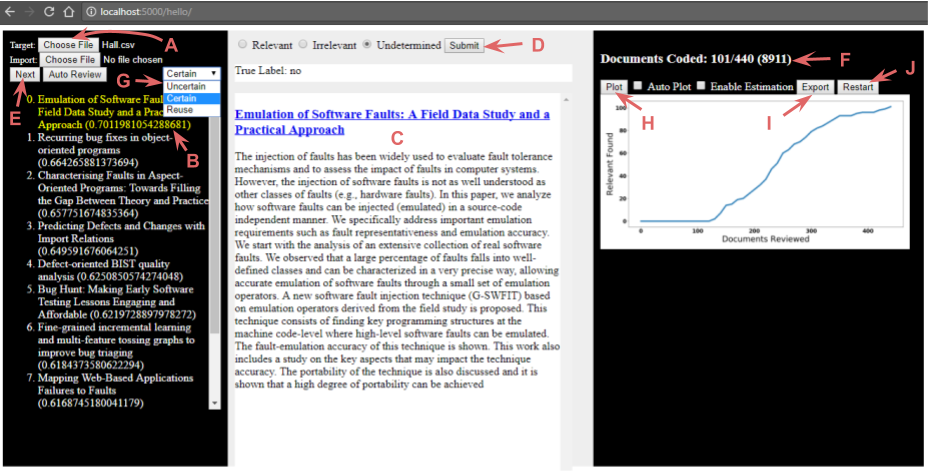
\includegraphics[width=\linewidth]{FASTREAD.png}
    \caption{Basic interface of the FASTREAD tool.}
    \label{fig:FASTREAD}
\end{figure*}


\begin{figure*}[!tbhp]
    \centering
    \subfloat[Input format]
    {
        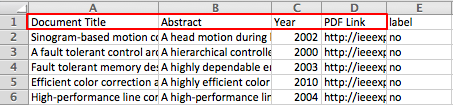
\includegraphics[width=0.48\linewidth]{Input.png}\label{fig:input}
    }
    \subfloat[Output format]
    {
        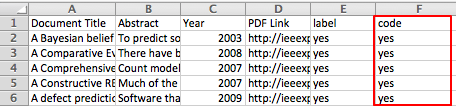
\includegraphics[width=0.48\linewidth]{Output.png}\label{fig:output}
    }    
    
    \caption{Data format for FASTREAD tool.}
    \label{fig:csv}
\end{figure*}

In order to implement FASTREAD, we developed a simple tool as shown in Fig.~\ref{fig:FASTREAD}. This software is freely available from SeaCraft Zenodo at \textit{https://doi.org/10.5281/zenodo.837861} and its Github repository at \textit{https://github.com/fastread/src}. 


Using FASTREAD, a review starts with \textbf{A}: selecting the input candidate study list from \textit{workspace/data/} directory. The input candidate list is specified in the format shown in Fig.~\ref{fig:input}. The input CSV file must have the \textit{Document Title}, \textit{Abstract}, \textit{Year}, and \textit{PDF Link} columns. The \textit{label} column, which is the true label of the candidate studies, is optional and is only used for testing. The output CSV file generated by the FASTREAD tool has an additional \textit{code} column, which is the reviewer-decided label for the candidate study. The final inclusion list can be retrieved by extracting all the studies with ``yes'' in the \textit{code} column.

The review then proceeds as follows:
\begin{enumerate}
\item[\textbf{B}] Randomly select $10$ candidate studies for review.
\item[\textbf{C}] Read through the title and abstract (and click on the title and read the full text if needed) of the candidate study.
\item[\textbf{D}] Decide whether this study should be coded as \textit{Relevant} or \textit{Irrelevant} and click the \textit{Submit} button.
\item[\textbf{E}] Click the \textit{Next} button and the codes are saved. Another $10$ candidate studies will be selected for review.
\item[\textbf{F}] The review status will change every time new studies are coded by reviewer and the \textit{Next} button is hit. The status is shown in the format ``Documents Coded: \textit{Number of relevant studies found} / \textit{Number of studies reviewed} (\textit{Total number of candidate studies}).''
\item[\textbf{G1}] Once \textbf{1} ``relevant'' study is coded, \textit{Random sampling} will be replaced by \textit{Uncertainty sampling}.
\item[\textbf{G2}] Once \textbf{30} ``relevant'' study is coded, \textit{Uncertainty sampling} can be changed to \textit{Certainty sampling}.
\item[\textbf{H}] Fig. can be plotted by clicking the \textit{Plot} button or checking \textit{Auto Plot}. The generated figure can also be found in the \textit{src/static/image/} directory. The new figure will overwrite any old one.
\item[\textbf{I}] Once finished, coded studies can be exported into a CSV file in the \textit{workspace/coded/} directory, in the format shown in Fig.~\ref{fig:output}.
\end{enumerate}

Note that the \textit{Restart} button (\textbf{J}) is only for testing and discards all codes.



\section{Threats to Validity}
\label{sect: Threats to Validity}

There are several validity threats to the design of this study~\cite{feldt2010validity}. Any conclusions made from this work must be considered with the following issues in mind:

{\em Conclusion validity} focuses on the significance of the treatment. To
enhance the conclusion validity of this work, we employed several statistical
tests (Scott-Knot) to reduce the changes of making spurious conclusions. 

{\em Internal validity} focuses on how sure we can be that the treatment
actually caused the outcome. To enhance our internal validity,
as far as possible, we heavily constrained our experiments
(see  our simulated in strictly controlled environments as discussed in Section~\ref{subsect: Controlled Variables}).

{\em Construct validity} focuses on the relation between the theory
behind the experiment and the observation. In this work, we evaluated
our results via different treatments with WSS@95 as stated in Section~\ref{subsect: Performance Metrics}-- note that those
measures took us as close as we can to computing
cost reduction without ``abstract relevant'' information. 
That is, it fits the objective of human-in-the-loop primary study selection as defined in the current literature~\cite{tredennick2015,cormack2015autonomy,cormack2014evaluation}. Increasing the number of different measures may increase construct validity
so, in future work, we will further explore more metrics.

{\em External validity }concerns how well the conclusion can be applied outside. All the conclusions in this study are drawn from the experiments running on three software engineering SLR datasets created with information from Hall, Wahono, Radjenovi{\'c} et al. studies~\cite{hall2012systematic,wahono2015systematic,radjenovic2013software} and one dataset provided by Kitchenham~\cite{kitchenham2010systematic}. Therefore, such conclusions may not be applicable to datasets of different scenarios, e.g., citation screening from evidence based medicine or TAR from e-discovery. Such bias threatens any classification experiment. The best any researcher can do is to document that bias then make available to the general research community all the materials used in a study (with the hope that other researchers will explore similar work on different datasets). Existing active learning techniques in citation screening have been criticized by Olorisade et al. for being not replicable~\cite{olorisade2016critical,olorisade2017reproducibility}. To this end, we have published all our code at \textit{https://github.com/fastread/src} and all our data at \textit{https://doi.org/10.5281/zenodo.837298}.

In the experiments, we assume that the human reviewer is always correct. In practice, this assumption cannot hold and problems such as disagreement between reviewers or concept drift (in which reviewers disagree with themselves as time passes) may occur.  As discussed
below when we discuss {\em Future Work}, we intend to explore this matter in the near future.

The comparisons in our experiment are based on the controlled variables listed in Section~\ref{subsect: Controlled Variables}. The conclusion in Section~\ref{subsect: Results} may become unreliable if any of the controlled variables changes.



\section{Conclusions}\label{sect: Conclusion}

Systematic literature reviews are the primary method for aggregating evidence in evidence-based software engineering. It is suggested for every researcher in software engineering to frequently conduct SLRs in~\cite{keele2007guidelines}. The hugest barrier to accomplish this is the cost. Usually an SLR would take months to finish and the conclusion drawn can be out of date in a few years. To tackle this barrier, this study focuses on primary study selection, one of the most difficult and time consuming steps in an SLR. Machine learning methods, especially active learning, are explored in our attempts to reduce the effort required to exclude primary studies. Three state-of-the-art active learning methods, two from evidence-based medicine and one from e-discovery, are analyzed and tested. In our experiments, we showed that by decomposing and reassembling the state-of-the-art treatments, a new treatment can be created which outperforms the state-of-the-art treatments and achieves a large cost reduction with 5\% recall lost.  

This work has lead to a simple software tool called FASTREAD, which
we described above in Section~\ref{sect: tool}. We are currently advertising
that tool on social media and hope that, very soon,
we will be  able to report on
case studies when other researchers use this tool. FASTREAD is
an open source tool, published in Github, and we also hope
that FASTREAD will be maintained and improved by numerous 
researchers exploring this kind of technology. 

\section{Future Work}
This study has several limitations as described in Section~\ref{sect: Frequently Asked Questions} and \ref{sect: Threats to Validity}. We plan to address those limitations in future work. Specific problems and plans for the future are listed below.

\begin{itemize}

\item
{\em Conclusions are drawn from three synthetic SLR datasets and one Kitchenham dataset.} Validate the generalizability of the results on different datasets, including datasets from evidence-based medicine and e-discovery.

\item
{\em Experiment results are evaluated by WSS@95, which assumes a stop rule of reaching 95\% recall.} How to stop at 95\% recall without first knowing the number ``relevant'' studies in the pool is an interesting topic. We are exploring this topic actively.

\item
{\em The size and prevalence of data can affect performance of FASTREAD.} The analysis of such effects may in return help estimate the prevalence, therefore makes it possible to estimate the total number of ``relevant'' studies in the pool.

\item
{\em About $10\%$ to $20\%$ efforts are spent on random selection step and most of the variances are also introduced in this step.} To speed up the random selection step, external expert knowledge will be introduced while unsupervised learning methods such as VTM or LDA will also be considered in future work. 

\item
{\em Some magic parameters are arbitrarily chosen, which may affect the performance.} However, parameter tuning is not a good fit for human-in-the-loop primary study selection because a) parameters should be tuned for the data working on; b) but the effect of applying different parameters can not be tested since querying extra label incurs extra cost. Therefore, novel methods should be explored for parameter selection; e.g. better criterion for when to switch from uncertainty sampling to certainty sampling (instead of the ``30'' relevant examples rule applied now).


\item
{\em Current scenario is restricted to having only one reviewer, which is impractical in practice.} Problems including how to assign review tasks to multiple reviewers and how to utilize reviewers with different cost and different capability will be explored in the future.

\item
{\em Current scenario assumes that reviewers never make mistakes, which is definitely not true in practice.} How to tackle concept drift (reviewers disagree with themselves) and how to settle disagreements (reviewers disagree with each other) would be valuable contributions for future work.

\item
{\em This study focuses only on primary study selection.} Assists on other steps of SLR such as searching, data extraction, and protocol development can also help reduce total effort of SLRs. The potential of combining VTM, snowballing, and other tools with FASTREAD needs to be explored as well.


\end{itemize}

 We invite other researchers to join us in the exploring the above. To that end, we have made all our tools and scripts readily available, on-line).

% With all the work in this study, a baseline result for human-in-the-loop primary study selection has now been established. There are still many concerns and potential improvements on FASTREAD, as discussed in Section~\ref{sect: Frequently Asked Questions}. We will keep working on the future work items and we believe that with all the materials in this work published, SE researchers can also explore further in SLR cost reduction. With our best hope, the effort required for conducting SLRs will eventually be reduced to days of work in the future and thus enable researchers to conduct SLRs much more frequently.

\section*{Acknowledgement}
The authors thank Barbara Kitchenham for
her attention to this work and for
sharing with us the ``Kitchenham'' dataset used in our experiments.
 
% \bibliographystyle{plain}
\bibliographystyle{spmpsci}
% \bibliography{sigproc} 
\documentclass{svjour3}
\usepackage{times}
\usepackage{blindtext, graphicx}

\usepackage{colortbl}
\usepackage{tikz}
\usepackage{microtype}
\def\firstcircle{(90:1.75cm) circle (2.5cm)}
\def\secondcircle{(210:1.75cm) circle (2.5cm)}
\def\thirdcircle{(330:1.75cm) circle (2.5cm)}
\smartqed

\usepackage{balance}
\definecolor{Gray}{rgb}{0.88,1,1}
\definecolor{Gray}{gray}{0.85}
\definecolor{lightgray}{gray}{0.8}
\setlength{\tabcolsep}{0.2em}


\usepackage{subfig} 



\usepackage{amsmath}
\DeclareMathOperator*{\argmin}{argmin}

\usepackage[framed]{ntheorem}
\usepackage{framed}
\usepackage{tikz}
\usetikzlibrary{shadows}
\theoremclass{Lesson}
\theoremstyle{break}

% inner sep=10pt,
\tikzstyle{thmbox} = [rectangle, rounded corners, draw=black,
fill=Gray!20,  drop shadow={fill=black, opacity=1}]
\newcommand\thmbox[1]{%
    \noindent\begin{tikzpicture}%w
    \node [thmbox] (box){%
        \begin{minipage}{.94\textwidth}%
        \vspace{-3mm}#1\vspace{-3mm}%
        \end{minipage}%
    };%
    \end{tikzpicture}}

\let\theoremframecommand\thmbox
\newshadedtheorem{lesson}{Finding}
\newcommand{\quart}[4]{\begin{picture}(80,4)%1
    {\color{black}\put(#3,2){\circle*{4}}\put(#1,2){\line(1,0){#2}}}\end{picture}}

\newcommand{\review}[1]{{\textit{#1}}~\\}
\newcommand{\todo}[1]{\textbf{\color{red}{#1}}}
\newcommand{\respto}[1]{
\fcolorbox{black}{black!15}{
\label{response:#1}
\bf
  \scriptsize R-{#1}}~
}
\newcommand{\citeresp}[1]{
{\bf (see } \fcolorbox{black}{black!15}{
 \bf
  \scriptsize R-{#1}}~{\bf{on page \pageref{response:#1})}}
}

%% space saving measures
% \usepackage[shortlabels]{enumitem}  
% \usepackage{url}

\begin{document}

\title{How to Read Less: On the Benefit of Active Learning for Primary Study Selection in Systematic Literature Reviews%\thanks{Grants or other notes
%about the article that should go on the front page should be
%placed here. General acknowledgments should be placed at the end of the article.}
}
% \subtitle{Do you have a subtitle?\\ If so, write it here}


% \pagenumbering{arabic} %XXX delete before submission

\author{Zhe Yu         \and
        Nicholas A. Kraft \and 
        Tim Menzies%etc.
}

%\authorrunning{Short form of author list} % if too long for running head

\institute{Zhe Yu \at
              Department of Computer Science, North Carolina State University, Raleigh, NC, USA \\
              \email{zyu9@ncsu.edu}           %  \\
%             \emph{Present address:} of F. Author  %  if needed
           \and
           Nicholas A. Kraft \at
              ABB Corporate Research, Raleigh, NC, USA\\
              \email{nicholas.a.kraft@us.abb.com}
            \and
           Tim Menzies \at
              Department of Computer Science, North Carolina State University, Raleigh, NC, USA \\
              \email{tim.menzies@gmail.com}
}

% \date{Received: date / Accepted: date}

\maketitle

\begin{abstract}
  
Systematic literature reviews (SLRs) are the primary method for aggregating and synthesizing evidence in evidence-based software engineering (SE). Primary study selection is a critical and time-consuming SLR step in which reviewers use
titles, abstracts, or even full texts to evaluate thousands of studies to find the dozens of them that are relevant to the research questions. We seek to reduce the effort of primary study selection in SE SLRs by exploring and refactoring the state-of-the-art active learning techniques from evidence-based medicine and legal electronic discovery. By refactoring those methods, we discovered FASTREAD, which is a new state-of-the-art in active learning for SE SLRs. When tested on four datasets generated from existing SE SLRs of Hall, Wahono, Radjenovi{\'c}, Kitchenham et al., FASTREAD outperformed the current state-of-the-art methods. Our results show that FASTREAD can save researchers much time during
 the literature review process (since they will need to review hundreds to thousands fewer abstracts ) 
 while sacrificing very little
in the final recall  (5\%).

\keywords{Active Learning\and Systematic Literature Review\and Software Engineering\and Primary Study Selection}

\end{abstract}



\section{Introduction}
\label{sect: Introduction}

The number of new publications every year is growing rapidly. For example, on defect
prediction, 729 studies were published on IEEE
Xplore\footnote{http://ieeexplore.ieee.org} during the year of 2005 while 1,564
studies were published during the year of 2015.
Given this increasingly faster pace of software engineering (SE) research,
it has become harder and harder to remain current with
the state-of-the-art research in software engineering.


\begin{figure*}[t]
    \centering
    \subfloat[Most Difficult Aspects of SLR Process.]
    {
        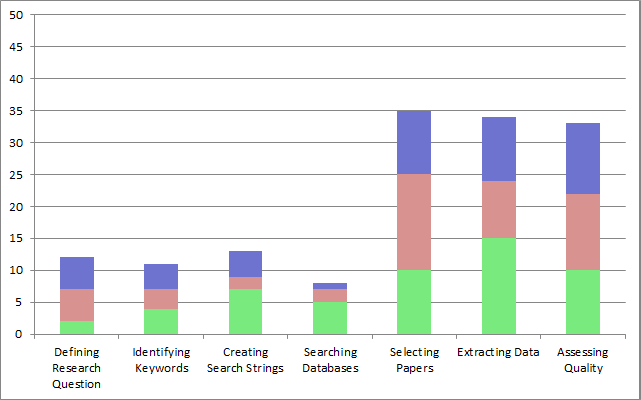
\includegraphics[width=0.48\linewidth]{difficulty.png}
        \label{fig: difficult}
    }
    \subfloat[Most Time Consuming Aspects of SLR Process.]
    {
        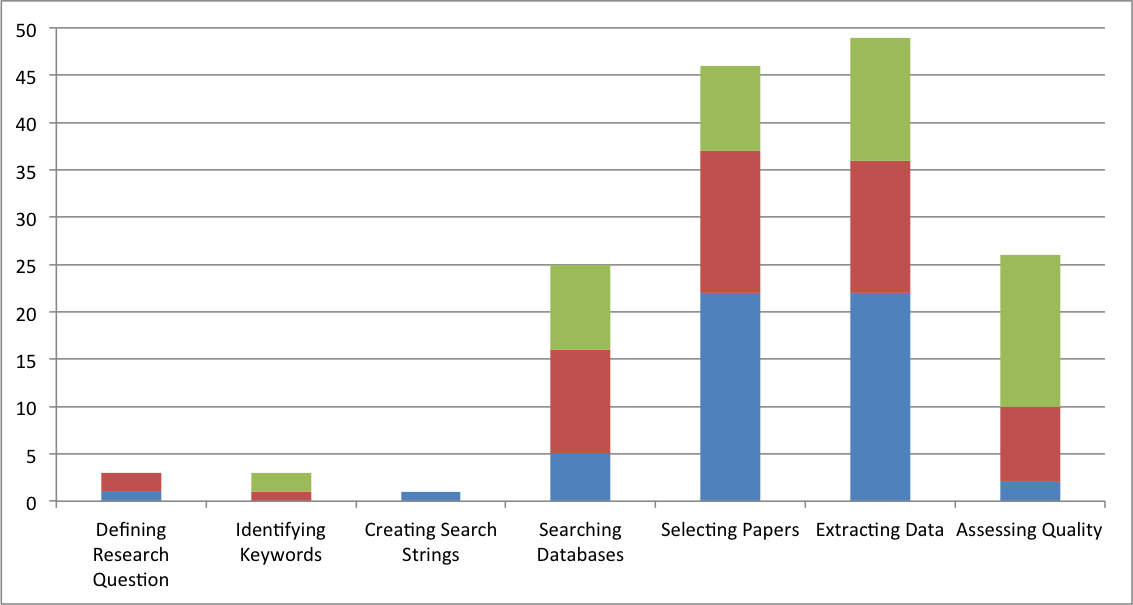
\includegraphics[width=0.48\linewidth]{time.png}
        \label{fig: time}
    }    
    \caption{Data collected from surveys to SLR authors~\cite{carver2013identifying}. Measured by number of votes, where {\setlength{\fboxsep}{1pt}\colorbox{green!40}{green}}, {\setlength{\fboxsep}{1pt}\colorbox{red!30}{red}}, and {\setlength{\fboxsep}{1pt}\colorbox{blue!50}{blue}} are number of times voted as most, second most, and third most, respectively.}
    \label{fig:barrier}
\end{figure*}
Systematic Literature Reviews
(SLRs) are one approach to this problem. SLRs are a well established and widely
applied review method in Software Engineering since Kitchenham, Dyb{\^{a}}, and
J{\o}rgensen first adopted it to support evidence-based software engineering in
2004 and 2005~\cite{kitchenham2004evidence,1377125}. 
Researchers can get a
general idea of current activity in their field of interests by reading the SLR
studies. Furthermore, a
deeper understanding of the topic may be gained by conducting an SLR.

An increasing number of SLRs has been conducted since the proposal and
revision of the SLR guidelines by Kitchenham in 2007~\cite{keele2007guidelines}. For
example, there were 26 SLRs on IEEE Xplore during the year of 2005 and that
number has increased to 137,199 for the years   2010,2015 (respectively). Various scholars  suggest that an SLR is required before any research in Software
Engineering is conducted~\cite{keele2007guidelines}.
While this is certainly a good advice,
currently an SLR is
a large, time consuming and complex
task~\cite{hassler2016identification,hassler2014outcomes,carver2013identifying,bowes2012slurp}.

Cost reduction in SLRs is therefore an important topic and will benefit researchers in software engineering community.
Previously we have analyzed the costs of SLRs~\cite{hassler2014outcomes,carver2013identifying}. As shown in Fig.~\ref{fig:barrier}, primary study selection, which is noted as ``selecting papers'' in Fig.~\ref{fig:barrier}, is among the top three most difficult
as well as time-consuming aspects in an SLR. Usually, reviewers need to evaluate
thousands of studies trying to find dozens of them that are relevant to the
research questions based on their title, abstract, or full text~\cite{bowes2012slurp}. An extreme
example of this is where reviewers sourced over
3,000 studies, and only used 7 of them in their final review~\cite{bezerra2009systematic}. The cost associated with primary study selection has become a serious problem and will continue to grow in the near future as the population of candidates for primary
studies increases dramatically. In this paper, we focus on reducing cost in primary study selection only. We prioritize primary study selection because there exists tool support for other time-consuming aspects such as searching databases~\cite{Molleri:2015:SWA:2745802.2745825,hernandes2012using}, extracting data\cite{Molleri:2015:SWA:2745802.2745825,hernandes2012using,fernandez2010slr,bowes2012slurp}, assessing quality~\cite{fernandez2010slr,bowes2012slurp,Molleri:2015:SWA:2745802.2745825}; and machine learning methods are promising in cost reduction for primary study selection~\cite{wallace2010semi,grossman2013}.

There are three main aspects in primary study selection: \textbf{(1)} retrieving initial list of primary studies, \textbf{(2)} excluding irrelevant studies, \textbf{(3)} including missing studies. We focus on excluding irrelevant studies because \textbf{a)} there already exists techniques and tools to facilitate \textbf{(1)} and \textbf{(3)} such as Snowballing~\cite{jalali2012systematic} and StArt~\cite{hernandes2012using}; \textbf{b)} the performance of excluding irrelevant studies can be evaluated using existing SLR publications.

In the SE research community, linear manual review, which requires reviewer to review every candidate study, is still the standard approach for primary study selection~\cite{kitchenham2013systematic}. On the other hand, machine learning algorithms, especially active learning, have been intensively studied to solve similar problems in other fields outside the SE research community in evidence-based medicine~\cite{paynter2016epc,wallace2010semi,wallace2010active} and in
legal electronic discovery~\cite{cormack2014evaluation,cormack2015autonomy}. This paper:
\begin{itemize}
\item
Reviews those methods. We find that in evidence-based medicine and legal electronic discovery, there are three widely recognized state-of-the-art active learning methods~\cite{cormack2014evaluation,wallace2010semi,miwa2014reducing}.
\item
Those three methods are assembled from four lower-level techniques including a) when to start training; b) query strategy; c) when/whether to stop training; d) data balancing. By analyzing techniques applied in the three methods, we generate 32 possible treatments.
\item
This paper explores all 32 treatments using data taken from the SE literature. Each treatment is evaluated by ``work saved over sampling at 95\% recall'' (WSS@95)~\cite{cohen2011performance}. 
\item
We find that one of those treatments, which we will call FASTREAD, robustly achieves the highest rank of performance across every dataset.
\end{itemize}
Interestingly, the FASTREAD treatment is not one of those used
in~\cite{cormack2014evaluation,wallace2010semi,miwa2014reducing}-- which is to say that the SE literature has nuanced differences to other kinds of literature and we should not just blindly
apply methods from other fields without certifying them on local data.
Using FASTREAD, hundreds to thousands of abstract reviewing can be avoided by sacrificing 5\% recall. That is, FASTREAD can dramatically reduce the cost of primary study selection in SE SLRs.

To assess those 32 treatments,
we need some ``gold sets'',
on which we can compare different combinations. Fortunately, in the arena of software engineering, there exist very prominent ``gold sets'' as published SLRs. This paper used three  primary study selection datasets by using the search strings and final inclusion list in such SLRs: Wahono et al. 2015~\cite{wahono2015systematic}, Hall et
al. 2012~\cite{hall2012systematic}, and Radjenovi{\'c} et al. ~\cite{radjenovic2013software}. These three SLRs are arbitrarily chosen from the set of SLR publications which define their work in enough details for us to construct datasets for simulations. Besides the three synthetic datasets, one set from Kitchenham et al. 2010~\cite{kitchenham2010systematic} has also been provided for the simulations. More details about the ``gold
sets'' will be presented later in Section~\ref{sect: datasets}. Using
these ``gold sets'', we ask and answer the following three research questions:

\begin{itemize}


\item
{\bf RQ1: Can active learning techniques reduce cost in primary study selection?} First of all, the effectiveness of active learning should be tested against traditional linear review. The rest of the research questions should not be investigated until active learning has been proved to be useful for cost reduction in primary study selection.

\item
{\bf RQ2: Should we just adopt the state-of-the-art treatments from other fields? Is it possible to build a better one by mixing and matching from those?} Active learning methods have been explored in other fields. Each of the state-of-the-art methods has its own advantage and thereby a better method might be derived by mixing and matching from those. 

\item
{\bf RQ3: How much effort can FASTREAD, our new state-of-the-art method for primary study selection, save in an SLR?} Details should be provided so that reviewers can decide whether to use FASTREAD or not.


\end{itemize}
The main contributions of this paper are:
\begin{itemize}
\item
  A demonstration of the value of  machine learning techniques for assisting primary study selection in SE SLRs.
\item
  The development of FASTREAD, a new state-of-the-art active learning method for primary study selection in SE SLRs, by refactoring three state-of-the-art methods from evidence-based medicine and electronic discovery.
  
\item
  The evaluation of our new method. The experiments shown below indicate that FASTREAD saves large amount of review efforts on primary study selection.
\item The development of a simple tool to implement FASTREAD for primary study selection.
  This tool is explained in Section~\ref{sect: tool} and is
  available for download on GitHub\footnote{https://github.com/fastread/src}. 
\end{itemize}










\section{Frequently Asked Questions}
\label{sect: Frequently Asked Questions}

When we discuss FASTREAD with our colleagues, several issues are commonly raised. This section discusses these issues.

\subsection{What about the other costs associated with SLRs?}

Our focus on the cost reductions of primary study selection is not to discount the effort associated with other parts of the SLR process. As mentioned in our introduction, we focus here on primary study selection since our data (from Fig.~\ref{fig:barrier}) indicates that this is a major component of SLR cost. 

In addition, there are tools support other components of SLRs and techniques facilitating primary study selection in different approaches. All these techniques (such as Quasi-Gold Standard based search~\cite{zhang2011empirical,zhang2011identifying}, visual text mining~\cite{Felizardo:2014:VAA:2601248.2601252,felizardo2012visual,felizardo2010approach,malheiros2007visual}, and snowballing~\cite{wohlin2014guidelines,jalali2012systematic}) are compatible and a better performance is expected when applied together. This leads to a direction of future work in which the best setting to integrate different techniques will be explored.

\subsection{What is missed?}

Our results will show, with FASTREAD, $95\%$ of the ``relevant'' studies can be retrieved by reviewing a small portion (usually hundreds of studies) of long candidate study list. Given that, it is wise to reflect
on the 5\% of papers {\em not} found by such an analysis. To this end, we took one of our case studies and reflected on:
\begin{itemize}
\item The set of papers $P_0$ that a human analyst declared to be ``relevant'' (as listed in their reference list at the end of their paper);
\item The {\em tangentially relevant} subset of those  papers $P_1 \subseteq P_0$ that a human analyst explicitly mentions, however briefly, in the body of their paper;
\item The yet smaller subset of those papers $P_2 \subseteq P_1$  that a human analyst discusses, at length, in the body of their report (and for
our purposes ``at length'' will be ``more that two lines''). We call these {\em insightful papers}. Clearly, FASTREAD should not be recommended if our method always misses the insightful papers, 
\end{itemize}
For the case studies shown below, on 30 repeats of our methods, we found that $|P_2|=0$; i.e. FASTREAD never missed an insightful paper. As for the tangentially
relevant papers, FASTREAD found all of those in 95\% of the 30 repeats. 
Based on this analysis, we infer that missing  $15\%$ of the papers is not a major impediment to using FASTREAD. Similar conclusion was derived by Shemilt et al. in 2016~\cite{shemilt2016use}.

That said, it is still true that if the SLR conductor does not want to miss any potential relevant study, he or she need to review all the candidate studies with full cost. We are actively exploring possibilities to mitigate or compensate the missing studies issue. 

% Data imbalance is explored further in Fioravanti and Nesi
% [[43]] and Zhang et al..

% Nikora and Munson [[126]] says that “without a widely agreed definition of severity
% we cannot reason about it” and Ostrand et al.
 

\subsection{What about domain knowledge?}

In our simulations, we assume that no initial seed training set is available thus a random sampling is performed to collect the minimum training set. This assumption represents the worst case while no external knowledge is available. We show in this work that the absence of that domain knowledge is not a critical failing of the approach. On the other hand, such domain knowledge usually exists in real world SLRs and will boost the performance of FASTREAD if wisely used. For example, if one relevant example and one irrelevant example are known in the very beginning, the random sampling step of FASTREAD is no longer needed and thus leads to additional cost reduction. More details about how to wisely use domain knowledge to boost FASTREAD will be explored further after this work. While we have some preliminary results in that area, we have nothing definitive to report at this time.

\subsection{What about real human reviewers?}

In our simulations, we assume that there is only one reviewer who never make mistakes. In real world SLRs, there will be multiple reviewers who make some mistakes. 

First, consider we have multiple reviewers but no mistakes. The schema of FASTREAD can be changed to one central learner with multiple review agents. Every agent reviews different studies and feedback his or her decisions to the central learner. The central learner then trains on the feedback of every agent and assigns studies to each agent for review. Such schema will keep all the property of single reviewer FASTREAD and performs similarly. In addition, there might be more intelligent way to allocate review tasks based on the different performance of review agents. Such possibility is worth exploring in future works and there already exists some studies on this topic in evidence-based medicine~\cite{wallace2011should}.

Second, consider those multiple reviewers now make mistakes. Candidate studies need to be reviewed by multiple reviewers in case any of them makes mistakes. To explore this issue, appropriate data need to be collected on how human reviewers make mistakes. Wallace et al. addressed this issue in~\cite{nguyen2015combining} by analyzing the best policy for allocating review tasks to reviewers with different experience levels as well as difference costs. We also plan to to address this issue in our future work.


\subsection{What about multiple categories of studies?}

In our simulations, we assume that the target is binary classification. However, primary study selection in real world SLRs might be a multi-label classification problem. For example, an SLR with two research questions might go through a primary study selection while each candidate is labeled as ``relevant to RQ1'', ``relevant to RQ2'', or ``irrelevant'' while the first two labels can co-exist. The simplest solution for this is to run multiple FASTREAD learners each learns on one label vs. others and each reviewer classify on one label only. In this case, the multi-label classification problem can be divided into multiple FASTREAD problems. Additional work such as ensemble learners can be explored in future works.

In summary, FASTREAD is an in-development technique that can be applied if the above trade-offs are acceptable. It can still be improved to further reduce cost of primary study selection and we will keep working on the issues until it becomes a reliable tool for different scenarios of SLRs.

























\section{Large Scale Literature Studies in SE}
\label{sect: Background}

\begin{figure}[t]
    \centering
    \begin{minipage}[t]{.51\linewidth}
    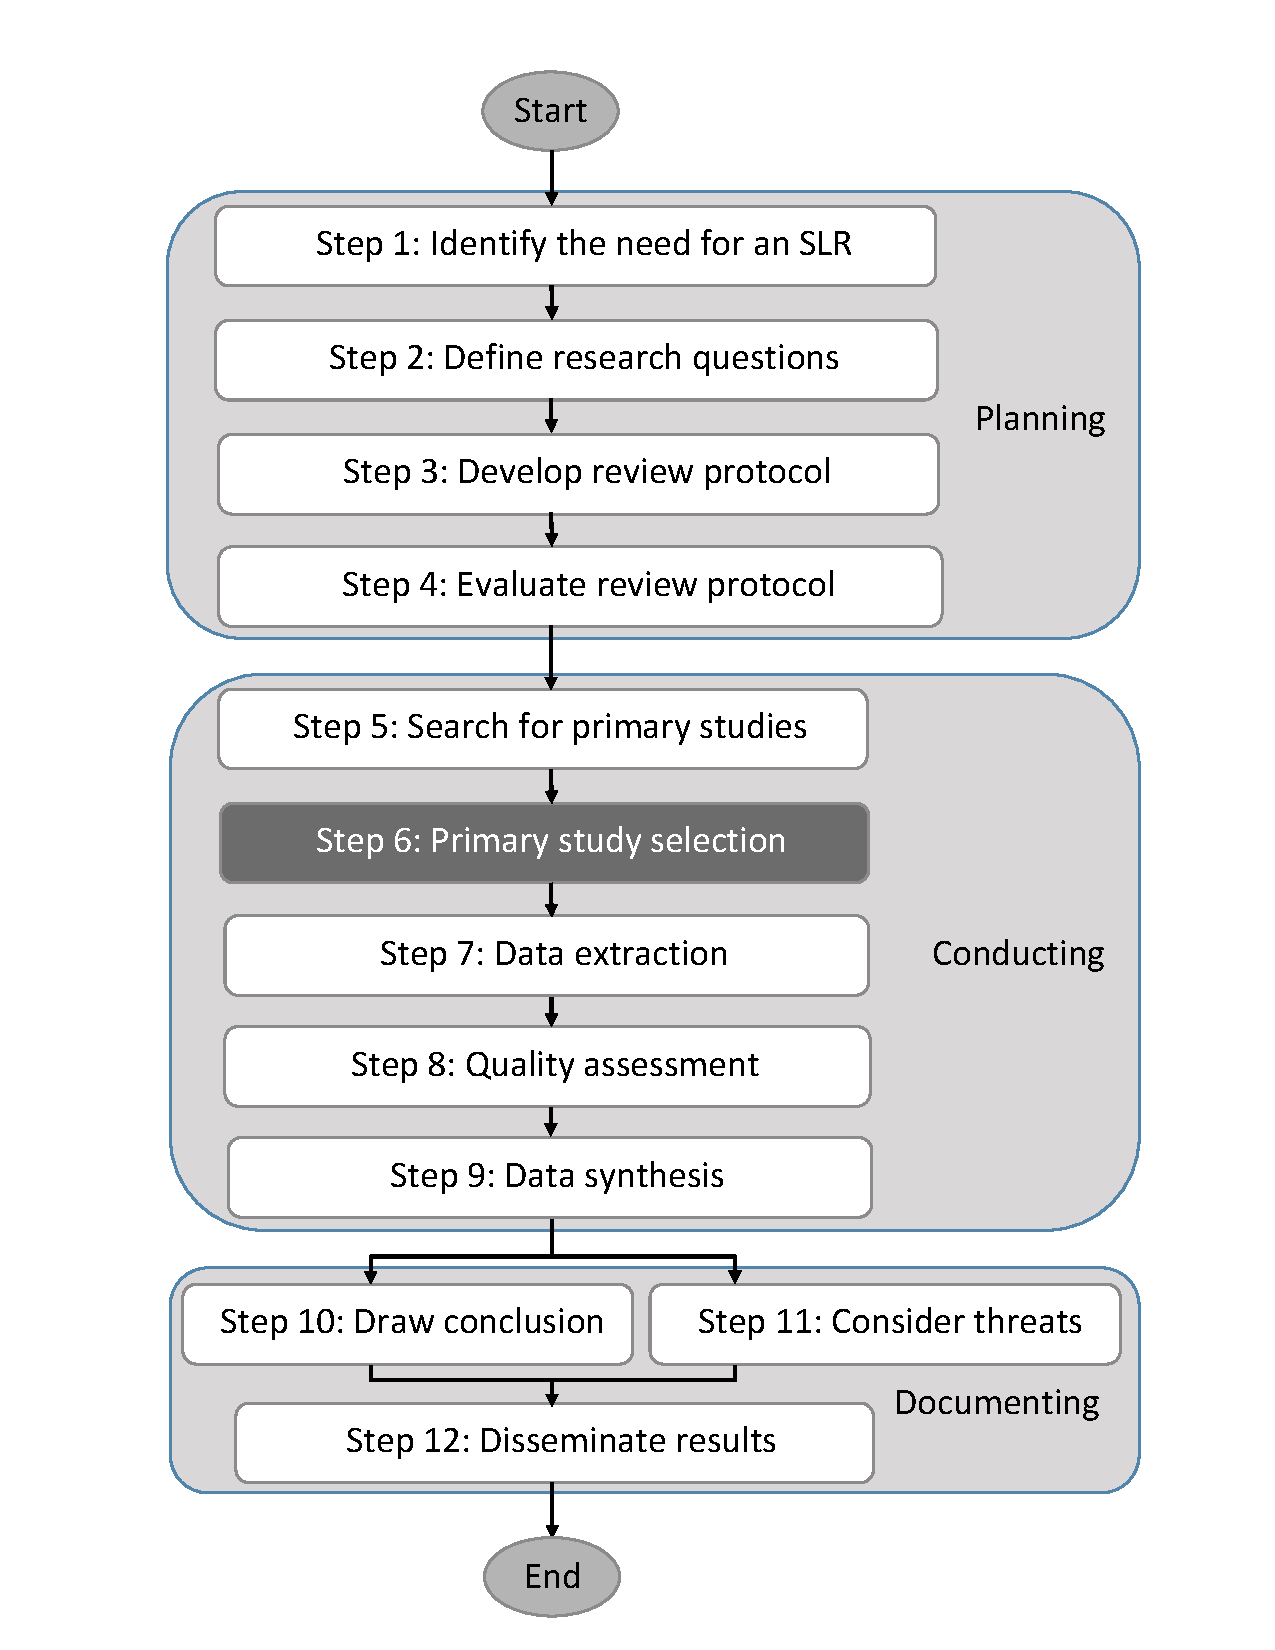
\includegraphics[width=\linewidth]{procedure.pdf}
    \caption{Systematic literature review steps suggested by~\cite{keele2007guidelines}. In this work, we focus on Step 6: primary study selection.}
    \label{fig: slr}
    \end{minipage}\quad
    \begin{minipage}[t]{.45\linewidth}
    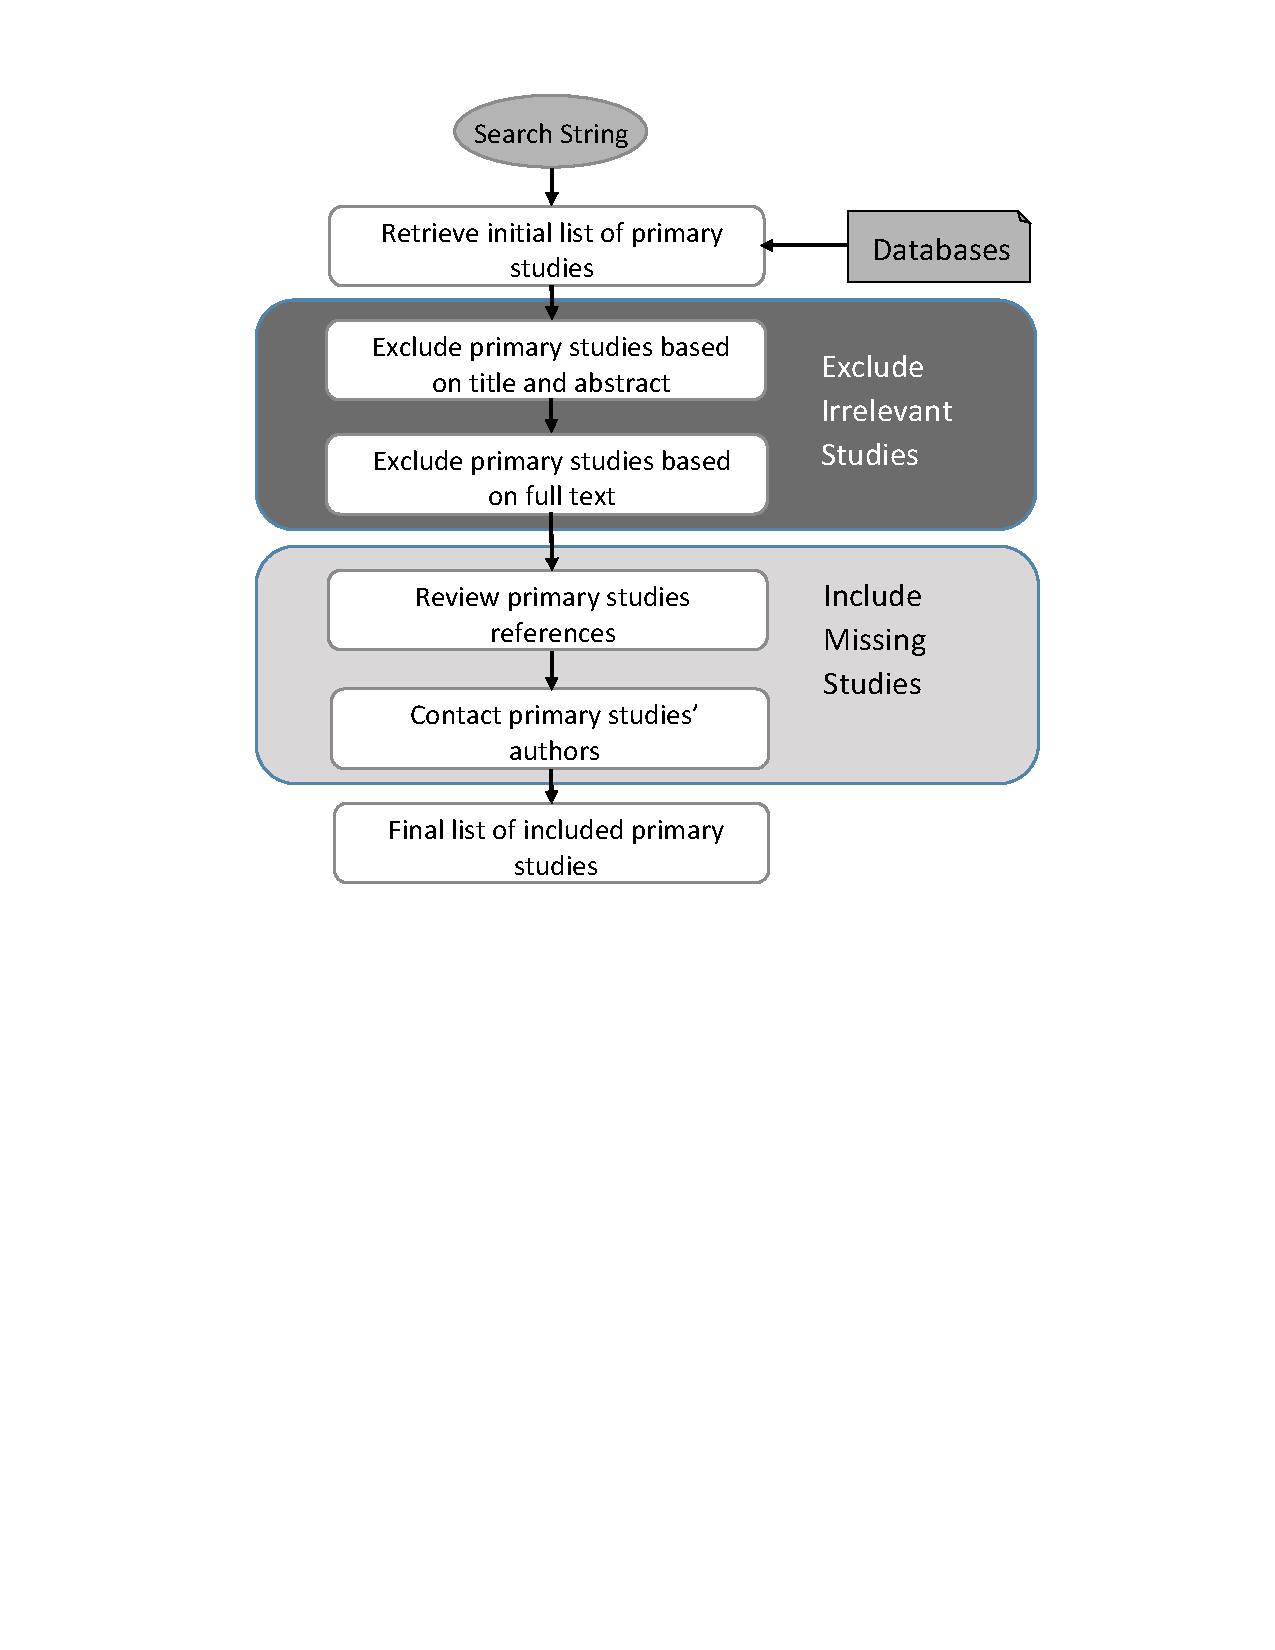
\includegraphics[width=\linewidth]{primary_study_selection.pdf}
    \caption{Primary study selection steps suggested by~\cite{keele2007guidelines}. In this work, we focus on the excluding irrelevant studies part.}
    \label{fig: prime}
    \end{minipage}
\end{figure}



% In contrast to a primary study, which investigates a specific research question,
% a systematic literature review is a form of secondary study aimed at
% identifying, evaluating and interpreting all available research relevant to a
% particular research question, topic area, or phenomenon of
% interest~\cite{keele2007guidelines}.
In the modern academic world, it is
impossible to start research without first knowing what other researchers have
done in the topic area. Conducting an SLR is one way to gain
background knowledge on a certain topic area.
If that SLR is published, then that paper becomes a useful research tool
for other researchers.  Kitchenham recommend SLRs to be standard
procedure in SE research~\cite{kitchenham2004evidence,keele2007guidelines}.

An SLR is usually conducted following the procedures in Fig.~\ref{fig: slr}. There can be variances on the real
implementations~\cite{wahono2015systematic,malhotra2015systematic,radjenovic2013software,unterkalmsteiner2012evaluation,hall2012systematic},
but all are based on the same guideline~\cite{keele2007guidelines}. Among all these steps, primary study selection is an important early step in SLRs. It starts with an initial candidate collection of studies retrieved by searching. In the first round of that process,
the reviewers' job is to read the titles and abstracts of candidate studies and classify each as ``relevant'' or ``irrelevant''. After the first round of review, the reviewers read through the full text of the previously included studies and make further decision on whether it is actually ``relevant'' or not. The whole procedure is shown in Fig.~\ref{fig: prime}. Typically, reviewers need to identify a final list of dozens of primary studies
among the initial collection of thousands of candidates. In terms of actual
cost, Malheiros has documented in~\cite{malheiros2007visual} that it requires 3
hours for one reviewer to review 100 studies.  This implies that it is a month's
work for one graduate student to review 3000 studies or three months' work to
review 9000 studies. 

In this work, we try to reduce the cost of the primary study selection by applying machine learning techniques to assist excluding irrelevant studies. In our {\em active learning} approach, each time a human reviews a paper, a learner updates its knowledge about what kind of documents are relevant. After that, the human uses that learned knowledge to guide the selection of the next paper to read.

The review cost of primary study selection can not be simply measured by the number of studies reviewed since the effort required for content review ($C_D$) is much higher than that for abstract review ($C_A$). Suppose one review process first identified $N_A$ ``relevant'' studies via reviewing $N$ abstracts, then reviewed the content of the $N_A$ studies and found $N_D$ of them are ``content relevant''. That is, to retrieve the $N_D$ ``content relevant'' studies, a total review cost of $C=N\times C_A+N_A\times C_D$ is required. To calculate this review cost, two level of relevance information is required (labels for ``abstract relevant'' and labels for ``content relevant''). However, most datasets of systematic literature review (including three datasets used in this study) have only one level of relevance information. As a result, only $N$ is used for review cost estimation since $N_A$ is not available. While this could be a fair metrics for comparing different treatments (smaller $N$ reflects less review cost in general), it is not a good estimation for how much effort saved by the text mining technique. Fortunately, the Kitchenham dataset provides two level of relevance information and we will explore the detailed review cost on this dataset in RQ3.





\subsection{Semi-Automated Tools for Literature  Reviews}

\subsubsection{Software Engineering Tools}

In recent years, various tools have been developed to facilitate SLRs in software engineering community, as summarized in~\cite{marshall2015tools,marshall2014tools,marshall2013tools}. These tools aim at providing support for protocol development~\cite{Molleri:2015:SWA:2745802.2745825,fernandez2010slr,hernandes2012using}, automated search~\cite{Molleri:2015:SWA:2745802.2745825,hernandes2012using}, primary study selection~\cite{Molleri:2015:SWA:2745802.2745825,hernandes2012using,fernandez2010slr,bowes2012slurp}, quality assessment~\cite{fernandez2010slr,bowes2012slurp,Molleri:2015:SWA:2745802.2745825}, data extraction and validation~\cite{Molleri:2015:SWA:2745802.2745825,hernandes2012using,fernandez2010slr,bowes2012slurp}, data synthesis~\cite{Molleri:2015:SWA:2745802.2745825,hernandes2012using,fernandez2010slr,bowes2012slurp},
and report write up~\cite{Molleri:2015:SWA:2745802.2745825,hernandes2012using,fernandez2010slr,bowes2012slurp}. It is extremely helpful to have a tool for managing the whole SLR process. However, the support for primary study selection using these tools is limited (e.g., to tasks such as assigning review jobs to multiple reviewers or to resolving disagreements).
Hence, we assert that the current SE SLR literature provides
no tool that can offer reductions in the effort required for primary study selection comparable to those reductions offered by active learning. Note that existing tools from Evidence-based Medicine offer active learning support and will be discussed in Section~\ref{sect: Evidence-based Medicine}.

Visual text mining (VTM) is a technique especially explored in Software Engineering community to support SLR. It is an unsupervised learning method which visualizes the relationship between candidate studies and helps the reviewer to make quick decisions. Malheiros et al.~\cite{malheiros2007visual} first applied VTM to support primary study selection in SLR. In their small-scale experiment (100 candidate studies, 31 of which are ``relevant''), VTM retrieves around 90\% of the ``relevant'' studies by spending about 30\% as much time as manual review. However, VTM requires some prior experience and knowledge of text mining and visualization techniques to use~\cite{bowes2012slurp}, and more case studies with large scale are needed to validate their results. 


Snowballing is another technique attracting much attention in SE SLR research. Given the inherent relevance relationship between a study and its citations, it is of high probability for the citations of (used in backward snowballing) and the studies cite (used in forward snowballing) a known ``relevant'' study to also be ``relevant''~\cite{kitchenham2004evidence}. Jalali and Wohlin~\cite{jalali2012systematic,wohlin2014guidelines} applied backward snowballing to search for primary studies in SE SLRs and found comparably good result as database search. Felizardo et al.~\cite{felizardo2016using} and Wohlin~\cite{wohlin2016second} applied forward snowballing to update SE SLRs and greatly reduced the number studies need to be reviewed comparing to a database search. This paper does not use snowballing since, as mentioned by Wohlin~\cite{wohlin2014guidelines}, snowballing starts with an initial set of relevant papers.
FASTREAD's task is very different: we start with zero relevant papers.



\subsubsection{Legal Electronic Discovery Tools}
\label{sect: Electronic Discovery}

Electronic Discovery (e-discovery) is a part of civil litigation where one party (the producing party), offers up materials which are pertinent to a legal case~\cite{krishna2016bigse}. This involves a review task where the producing party need to retrieve every ``relevant'' document in their possession and turn them over to the requesting party. It is extremely important to reduce the review cost in e-discovery since in a common case, the producing party will need to retrieve thousands of ``relevant'' documents among millions of candidates. Technology-assisted review (TAR) is the technique to facilitate the review process. The objective of TAR is to find as many
of the ``relevant'' documents in a collection as possible, with reasonable cost~\cite{grossman2013}. Various machine learning algorithms have been studied in TAR. So far, in every controlled studies, continuous active learning has outperformed others~\cite{cormack2014evaluation,cormack2015autonomy}, which makes it the state-of-the-art method in legal electronic discovery. It has also been selected as a baseline method in the total recall track of TREC 2015~\cite{roegiest2015trec}. Details on continuous active learning will be provided in Section~\ref{sect: Continuous Active Learning}. 

% Interestingly, the relationship between e-discovery and evidence-based medicine have been discussed in~\cite{leasesystematic} but their methods are still diverged. Relying on Grossman and Cormack~\cite{grossman2013} for support, many legal service providers have adopted TAR to facilitate the review process.

% In summary: the state-of-the-art active learning techniques are patient active learning in evidence-based medicine and continuous active learning in e-discovery.

\subsubsection{Evidence-based Medicine Tools}
\label{sect: Evidence-based Medicine}

Systematic literature reviews were first adopted from evidence-based medicine in
2004~\cite{kitchenham2004evidence}. To facilitate citation screening (primary
study selection) in systematic review, many groups of researchers have investigated different types of machine learning algorithms and evaluation mechanisms~\cite{o2015using,paynter2016epc}. 

Cohen et al. first applied text mining techniques to support citation screening and developed several performance metrics (including WSS) for assessing the performance of different techniques in 2006~\cite{cohen2006reducing}. While the great contribution of introducing machine learning and text mining into citation screening as well as the proposed performance metrics of Cohen has been widely acknowledged~\cite{o2015using}, most of Cohen's work focused on supervised learning which does not utilize unlabeled data and relies on random sampling to obtain the sufficiently large training set~\cite{cohen2006reducing,cohen2006effective,cohen2010prospective,cohen2011performance}.

Wallace et al. conducted a series of studies
with machine learning techniques, especially active
learning~\cite{wallace2010semi,wallace2010active,wallace2011should,wallace2012deploying,wallace2013active,wallace2013modernizing,nguyen2015combining}. Wallace
first set up a baseline approach called ``patient active learning'' (PAL), which will be explained later in this subsection, for machine learning assisted citation screening~\cite{wallace2010semi}. The performance of patient active learning is good enough (nearly 100\% of the ``relevant''
citations can be retrieved at half of the conventional review cost) to convince
systematic review conductors to adopt machine learning assisted citation
screening. Instead of improving this baseline method, Wallace then focused on other aspects of machine learning assisted citation screening such as introducing external expert knowledge~\cite{wallace2010active}, allocating review tasks to multiple experts~\cite{wallace2011should} or to crowdsourcing workers~\cite{nguyen2015combining}, and building a tool called abstrackr to provide overall support~\cite{wallace2012deploying}. Wallace's work on this topic is of exemplary high-impact and his core algorithm   (on simple expert screening),   is one of the most popular active learning techniques we have found in the evidence-based medical literature. That said, this technique has not been updated since 2010~\cite{wallace2010semi}. In this paper we are focused on the core active learning algorithm for cost minimization. Hence, we do not explore techniques such as Wallace's use of multiple experts (but in future work, we will explore this approach).

More recent work of Miva et al. explored alternative data balancing and query strategy in 2014~\cite{miwa2014reducing} and proposed a new treatment of Certainty plus Weighting. Instead of uncertainty sampling in PAL (and most conventional active learning approaches), Miva found that certainty sampling provides better results in clinical citation screening tasks. Similar conclusion for data balancing method as weighting relevant examples was found to be more effective than aggressive undersampling. Although not stated explicitly, Certainty plus Weighting keeps training until all ``relevant'' studies have been discovered, which differs from the stopping criteria of PAL. Aside from the core algorithm, additional views from latent Dirichlet allocation (LDA) has been found to be potentially useful.

Other work related to machine learning assisted citation screening do not
utilize active learning and active learning. Pure supervised learning requires a sufficiently large training set, which leads to a huge review cost~\cite{cohen2006reducing,adeva2014automatic}. Semi-supervised learning~\cite{liu2016comparative} does not utilize the human reviewers' feedback for updating the model, which leads to a depreciated performance in a long run. As a result, the patient active
learning proposed by Wallace et al.~\cite{wallace2010semi} and the Certainty plus Weighting approach by Miwa et al.~\cite{miwa2014reducing} are still considered to be the state-of-the-art method for citation screening in the scenario with no external knowledge and equally expensive reviewers. Details on these two approaches will be provided in Section~\ref{sect: Patient Active Learning} and \ref{sect: Certainty plus Weighting}.

There are also existing tools to support study selection in systematic reviews, e.g. Abstrakr\footnote{http://abstrackr.cebm.brown.edu}~\cite{wallace2012deploying}, EPPI-Reviewer\footnote{http://eppi.ioe.ac.uk/cms/er4/}~\cite{thomas2010eppi}, Rayaan\footnote{http://rayyan.qcri.org/}~\cite{Ouzzani2016}. Amazing features can be found in these tools such as a) Rayaan and EPPI-Reviewer: incorporated keyword search in screening; b) Rayaan and EPPI-Reviewer: deduplication; c) Rayaan and EPPI-Reviewer: define inclusion/exclusion criteria by terms; d) Abstrakr: user defined tags; e) all three: assign review tasks to multiple reviewers; f) all three: automatically extract data from PubMed. However, the active learning parts alone in these tools are depreciated. Under the condition that no additional feature (search, tags, define inclusion/exclusion terms) is used, we tried all three tools with one of our dataset-- Hall set (106 relevant in 8911 studies) and after reviewing 1000 studies, only 10 to 15 relevant ones were found, which was very close to a random sampling result without any learning. Since none of these tools are open-source, we cannot tell whether active learning is applied or how/when it is applied in each tool. This motivates us to develop an open source tool which focuses on active learning to support the primary study selection process. Details about our tool will be presented in Section~\ref{sect: tool}.



\section{Technical Notes}
\label{sect: Technical Briefing}

\begin{figure}[!t]
    \centering
    \subfloat[SVM without data balancing]
    {
        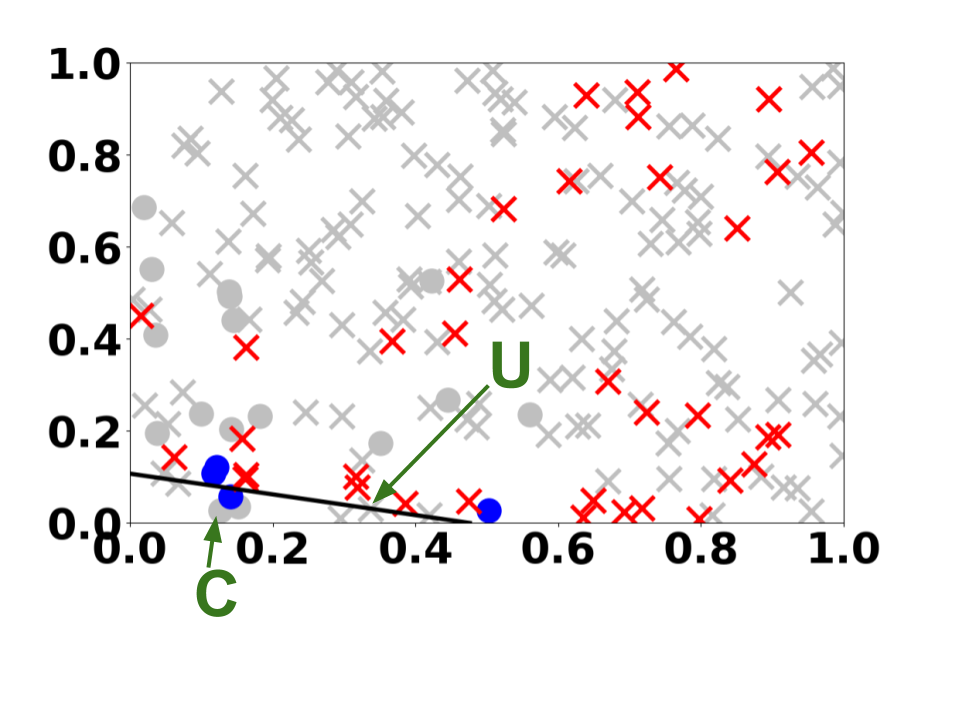
\includegraphics[width=0.3\linewidth]{simu22.png}
        \label{fig:train}
    }
    \subfloat[SVM with aggressive undersampling]
    {
        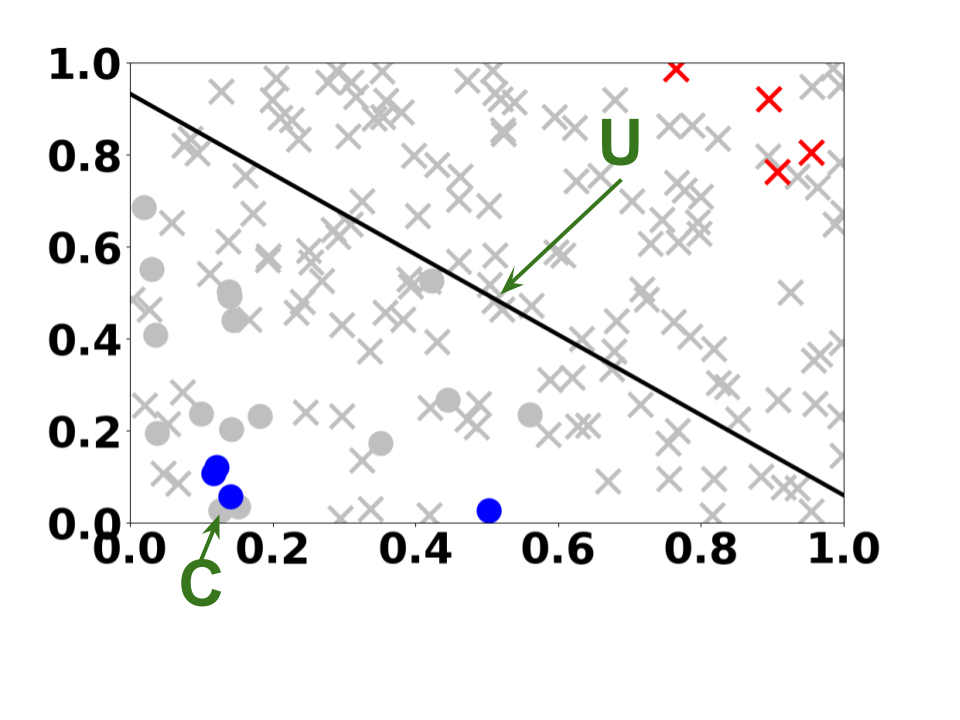
\includegraphics[width=0.3\linewidth]{simu23.png}
        \label{fig:train_a}
    }
    \subfloat[SVM with Weighting]
    {
        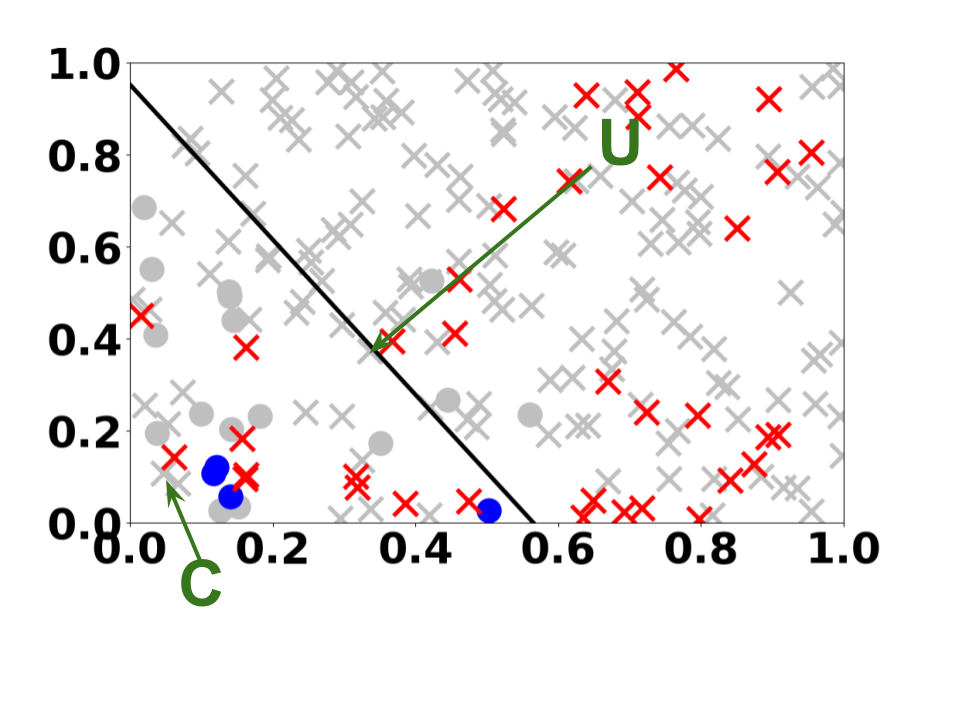
\includegraphics[width=0.3\linewidth]{simu24.png}
        \label{fig:test}
    }

    \caption{A demonstration of how SVM model is trained on imbalanced data, where ``$O$'' is the minority class, ``relevant'' studies in SLR, ``$X$'' is the majority class, ``irrelevant'' studies in SLR, markers in gray are the unlabeled studies, and black line is SVM decision plane. In (b), aggressive undersampling balances the training data by throwing away majority class examples closest to the old decision plane in (a). In (c) Weighting balances the training data by putting more weight on the minority class examples. Uncertainty sampling returns the unlabeled examples closest to the decision plane while certainty sampling returns the unlabeled examples furthest to the decision plane from the bottom-left side.}
    \label{fig:SVM}
\end{figure}

In this section, we provide details on technical terms 
used in the paper,  along with some brief introductory
notes on machine learning techniques used in this study.


\subsection{Linear Review}
\label{sect: Linear Review}

Linear review lets the reviewer to review and label every candidate study in a random order. This is still the most popular review method when there is unlimited review budget and completeness is the major objective. In this study, linear review works as a baseline method where no text mining technique is applied.

\subsection{Support Vector Machine}
\label{sect: Support Vector Machine}

Support vector machines (SVM) are a well-known and widely used classification method. The idea behind is to map input data to a high-dimension feature space and then construct a linear decision plane in that feature space~\cite{cortes1995support}. Linear SVM~\cite{joachims2006training} has been proved to be a useful model in SE text mining~\cite{krishna2016bigse} and is applied in the state-of-the-art active learning methods of both evidence-based medicine and electronic discovery~\cite{miwa2014reducing,wallace2010semi,cormack2014evaluation}. Fig.~\ref{fig:SVM} illustrates how linear SVM model is trained on a two-dimension feature space with different data balancing techniques.

\subsection{Active Learning}
\label{sect: Active learning}

Active learning is a cost-aware machine learning algorithm where labels of training data can be acquired with certain costs. The key idea behind active learning is that a machine learning algorithm can perform better with less
training if it is allowed to choose the data from which it learns~\cite{settles2012active}. There are several scenarios active learning is applied to, such as membership query synthesis, stream-based selective sampling, and pool-based sampling~\cite{settles2010active}. There are also different query strategies of active learning, such as uncertainty sampling, query-by-committee, expected model change, expected error reduction, variance reduction, and density-weighted methods~\cite{settles2010active}. Here, we will briefly introduce one scenario and two query strategies, which will be used in our later experiments and discussions.

\textbf{Pool-based sampling} is the scenario of primary study selection. This scenario starts with a fixed size pool of unlabeled data. Labels for the data can be acquired by querying an oracle selectively. The goal of pool-based sampling is to select the most informative data in the pool for query, thereby building a better model with less training.

\textbf{Uncertainty sampling} is the query strategy utilized in the state-of-the-art active learning technique of evidence-based medicine~\cite{wallace2010semi,wallace2010active}. It is also recognized as the most simple and commonly used query strategy~\cite{settles2010active}. In this query strategy, uncertainty sampling queries the instances about which the learner is least certain how to label. These instances are those (a) whose posterior probability of being positive are nearest 0.5 in probabilistic models or (b) closest to the decision boundary in models such as SVM. 

\textbf{Certainty sampling} is another query strategy which is applied in the state-of-the-art active learning technique of electronic discovery~\cite{cormack2014evaluation,cormack2015autonomy} and is also preferred over uncertainty sampling by Miwa et al. \cite{miwa2014reducing}. In contrast to uncertainty sampling, certainty sampling queries the instances about which the learner is most certain to label as positive. These instances are those (a) whose posterior probability of being positive are highest in probabilistic models, or (b) lies in the positive side of the decision boundary and furthest to the decision boundary in models such as SVM. This query strategy is usually NOT used when building the classifier of active learning since it is commonly believed that examples queried by certainty sampling contains less information than those by uncertainty sampling.

% \subsection{active Learning}
% \label{sect: active Learning}

% active learning is a combination of human decisions and machine
% suggestions~\cite{tredennick2015}. In this approach:
% \begin{itemize}
% \item
% Humans read a stream of documents, commenting on whether or
% not each one is ``relevant''.
% \item
%   Machine learners use feedback from the human opinion to
%   incrementally update their models actively.
% \item
%   The models generated via machine learning are used
%   to sort the stream of documents such that the humans focus on the
%   most informative documents.
%   \end{itemize}

% This is a
% pool-based active learning scenario since \textbf{a)} the process starts with a fixed size candidate list without any labels and \textbf{b)} training examples gradually become available to the learner as the human reviewer reviews the documents.  However, an important difference between active learning and other active learning methods is that every document labeled as ``relevant'' has been reviewed by a human. The machine never makes the final decision on whether a document is ``relevant''; a human makes such decisions and the machine only suggests a review order based on the human input. As a result, instead of building a better classification model, the objective of active learning is to retrieve most ``relevant'' documents from a pool of candidates while manually reviewing as few documents as possible. 

% Simple active learning, which is pool-based active learning with uncertainty sampling~\cite{settles2012active}, is the most basic form of learning methods
% applied to active learning. Although simple active learning achieves
% satisfactory performance, it has been outperformed by the state-of-the-art active learning techniques in both evidence-based medicine~\cite{wallace2010semi} and electronic discovery~\cite{cormack2014evaluation}. 


\subsection{Patient Active Learning}
\label{sect: Patient Active Learning}

One of the state-of-the-art active learning method in evidence-based medicine, patient active learning (PAL) can be described as following~\cite{wallace2010semi}:

\begin{itemize}

\item
{\bf Stage I: Construct an initial seed training set} by randomly sampling from the candidate study pool and asking a human reviewer to label the sampled papers as ``relevant'' or ``irrelevant''. Stop and proceed to Stage II when \textit{enough} ``relevant'' studies have been retrieved to represent the ``relevant'' class. (Note that Wallace et al.~\cite{wallace2010semi} did not provide an explicit definition of \textit{``enough''}.)

\item
{\bf Stage II: Build the classifier}, which is a linear SVM, by repeatedly training on labeled studies and uncertainty sampling. Unlabeled studies in the pool will be ranked in the descending order of uncertainty (uncertainty sampling). The human reviewer labels the studies in the ranked order and feeds them back to retrain the classifier. Stop and proceed to Stage III when the classifier is \textit{stable}. (Note that Wallace et al.~\cite{wallace2010semi} did not provide an explicit definition of \textit{``stable''}.)

\item
{\bf Stage III: Prediction.} Retrain the classifier with \textbf{aggressive undersampling} and then stop training. Unlabeled studies in the pool will be ranked in the descending order of the classifier's prediction probability of being ``relevant'' (certainty sampling as discussed in Section~\ref{sect: Active learning}). The human reviewer labels the studies in the ranked order until finished (running out of review cost budget, enough ``relevant'' studies found, or no more ``relevant'' studies are detected in multiple rounds).

\end{itemize}

{\bf Aggressive undersampling: }The data for citation screening are (at times, extremely) imbalanced, i.e., the prevalence of ``relevant'' citations is always smaller than $50\%$ (and often much smaller). Classification algorithms are typically optimized for overall accuracy, rather than accuracy, precision, recall to a particular class. This becomes a problem when only the performance on a minority class matters. Patient active learning utilizes aggressive undersampling for data balancing. By throwing away majority (``irrelevant'') class training examples which are closest to the SVM decision hyperplane, it undersamples the majority class training examples to the same size as minority (``relevant'') class. It is a recall friendly undersampling method since the new decision hyperplane is pushed away from the minority class. An exampling of aggressive undersampling is shown in Fig.~\ref{fig:SVM}.

\subsection{Certainty plus Weighting}
\label{sect: Certainty plus Weighting}

Another state-of-the-art active learning method in evidence-based medicine, Miwa et al. suggested using certainty sampling and weighting instead of uncertainty sampling and aggressive undersampling in PAL. This method can be described as following~\cite{miwa2014reducing}:

\begin{itemize}

\item
{\bf Stage I: Construct an initial seed training set} by randomly sampling from the candidate study pool and asking a human reviewer to label the sampled papers as ``relevant'' or ``irrelevant''. Stop and proceed to Stage II when \textit{enough} ``relevant'' studies have been retrieved to represent the ``relevant'' class. (Same as PAL.)

\item
{\bf Stage II: Build the classifier}, which is a linear SVM, by repeatedly training on labeled studies with \textbf{Weighting} and certainty sampling. Unlabeled studies in the pool will be ranked in the classifier's prediction probability of being ``relevant''(certainty sampling). The human reviewer labels the studies in the ranked order and feeds them back to retrain the classifier. Training continues until finished (running out of review cost budget, enough ``relevant'' studies found, or no more ``relevant'' studies are detected in multiple rounds).

\end{itemize}

{\bf Weighting: }Weighting balances the training examples by putting more weights on the minority class. The weighting factor is calculated as \emph{Size of Majority Class Training Examples / Size of Minority Class Training Examples}. An exampling of Weighting is shown in Fig.~\ref{fig:SVM}.

Miwa et al. also suggested that clustering by LDA before review has the potential to provide better performance in certain situations. However, this study focuses on refactoring and comparing the core active learning methods, same preprocessing step (without LDA) is applied to every treatment. The exploration of different feature engineering and preprocessing are planned for future works.

\subsection{Continuous Active Learning}
\label{sect: Continuous Active Learning}

The state-of-the-art active learning method in e-discovery, continuous active learning (CAL) can be described as following~\cite{cormack2014evaluation,cormack2015autonomy,tredennick2015}:

\begin{itemize}

\item
{\bf Stage I: Construct an initial seed training set} by random sampling from the candidate study pool and ask a human reviewer for labels. Stop and proceed to Stage II as soon as \textbf{ONE} ``relevant'' study is retrieved.

\item
{\bf Stage II: Predict and retrain} by repeatedly training on labeled studies and certainty sampling. Unlabeled studies in the pool will be ranked in the descending order of the classifier's prediction probability of being ``relevant'' (certainty sampling). A human reviewer labels the studies in the ranked order and feeds them back to retrain the classifier until finished.

\end{itemize}

In contrast to PAL, CAL is the opposite of ``patient''. It starts to train the model as soon as \textit{ONE} ``relevant'' study shows up and skips the uncertainty sampling stage, which is believed to be essential for active learners~\cite{settles2012active}. Since the objective is to retrieve ``relevant'' studies with candidates reviewed as few as possible, it is reasonable not to waste any single effort on building up the classifier~\cite{cormack2014evaluation,tredennick2015}. Also, the experiment results in~\cite{cormack2014evaluation} has demonstrated the value of this ``greedy'' strategy.

Among all the three state-of-the-art treatments, CAL and PAL are different in every aspect while Certainty plus Weighting is in the middle of these two and supports a different data balancing method.


\section{Methods}
\label{sect: Method}

This section describes our datasets and their preparation then describes and refactors state-of-the-art methods for active learning.
This refactoring process will create FASTREAD, our preferred active learning
method. 

\subsection{Datasets}
\label{sect: datasets}

Although a large number of SLRs are published every year, there is no dataset clearly documenting the details in primary study selection. As a result, three datasets are created based on the information in existing SLRs and being used in this study to simulate the process of excluding irrelevant studies. The three datasets are named after the authors of their original publication source-- Wahono dataset from Wahono et al. 2015~\cite{wahono2015systematic}, Hall dataset from Hall et al. 2012~\cite{hall2012systematic}, and Radjenovi{\'c} dataset from Radjenovi{\'c} et al. 2013~\cite{radjenovic2013software}. 

For each of the datasets, the search string \textbf{S} and the final inclusion list \textbf{I} from the original publication are used for the data collection. We retrieve the initial candidate collection \textbf{C} from IEEE Xplore with the search string (slightly modified to meet the requirement of IEEE Xplore). Then make a final list of inclusion \textbf{R} as \textbf{R} = \textbf{I} $\cap$ \textbf{C}. Here, for simplicity reason we only extract candidate studies from IEEE Xplore. We will explore possibilities for efficiently utilizing multiple data sources in the future work but in this paper, without loss of generality, we only extract initial candidate list from single data source. In this way, we created three datasets that reasonably resemble real SLR selection results assuming that any study outside the final inclusion list \textbf{I} is irrelevant to the original SLRs. A summary of the created datasets is presented in Table~\ref{tab: number}.

Apart from the three created datasets, one dataset (Kitchenham) is provided directly by the author of Kitchenham et al. 2010~\cite{kitchenham2010systematic} and includes two levels of relevance information. In general, only the ``content relevant'' labels are used in experiments for a fair comparison with other datasets. Additionally, the ``abstract relevant'' labels are used for detailed review cost analysis in RQ3. Summary of Kitchenham dataset is also presented in Table~\ref{tab: number}.

All the above datasets are available on-line at {\em https://doi.org/10.5281/zenodo.837298}.

\begin{table}
\caption{Descriptive statistics for experimental datasets}
\label{tab: number}
\begin{center}
\begin{tabular}{ |l|c|c|c|c| }
  \hline
   Datasets & \multicolumn{2}{|c|}{Generated} & \multicolumn{2}{|c|}{Original} \\
  \cline{2-5}
  & \#Candidate $|$\textbf{C}$|$ & \#Relevant $|$\textbf{R}$|$& \#Candidate & \#Relevant $|$\textbf{I}$|$\\
  \hline
  Wahono & 7002 & 62 & 2117 & 72\\
  \hline
  Hall & 8911 & 106 & 2073 & 136 \\
  \hline
  Radjenovi{\'c} & 6000 & 48 & 13126 & 106\\
  \hline
  Kitchenham & 1704 & 44 (132) & 1704 & 44 (132) \\
  \hline
\end{tabular}
\end{center}
{\footnotesize Our datasets are generated using information in the original SLR literature. Our candidate studies are retrieved by applying similar if not the same the search string from original SLR literature and search in IEEE Xplore. The set of our relevant studies is the intersection of the set of our candidate studies and the set of final included studies in the original SLR literature. Kitchenham dataset is different as it is provided directly by Kitchenham and it has two level of relevance labels-- 132 relevant studies by title and abstract review and within which, 44 relevant studies by content review.}
\end{table}




\begin{figure}[t]
    \centering
    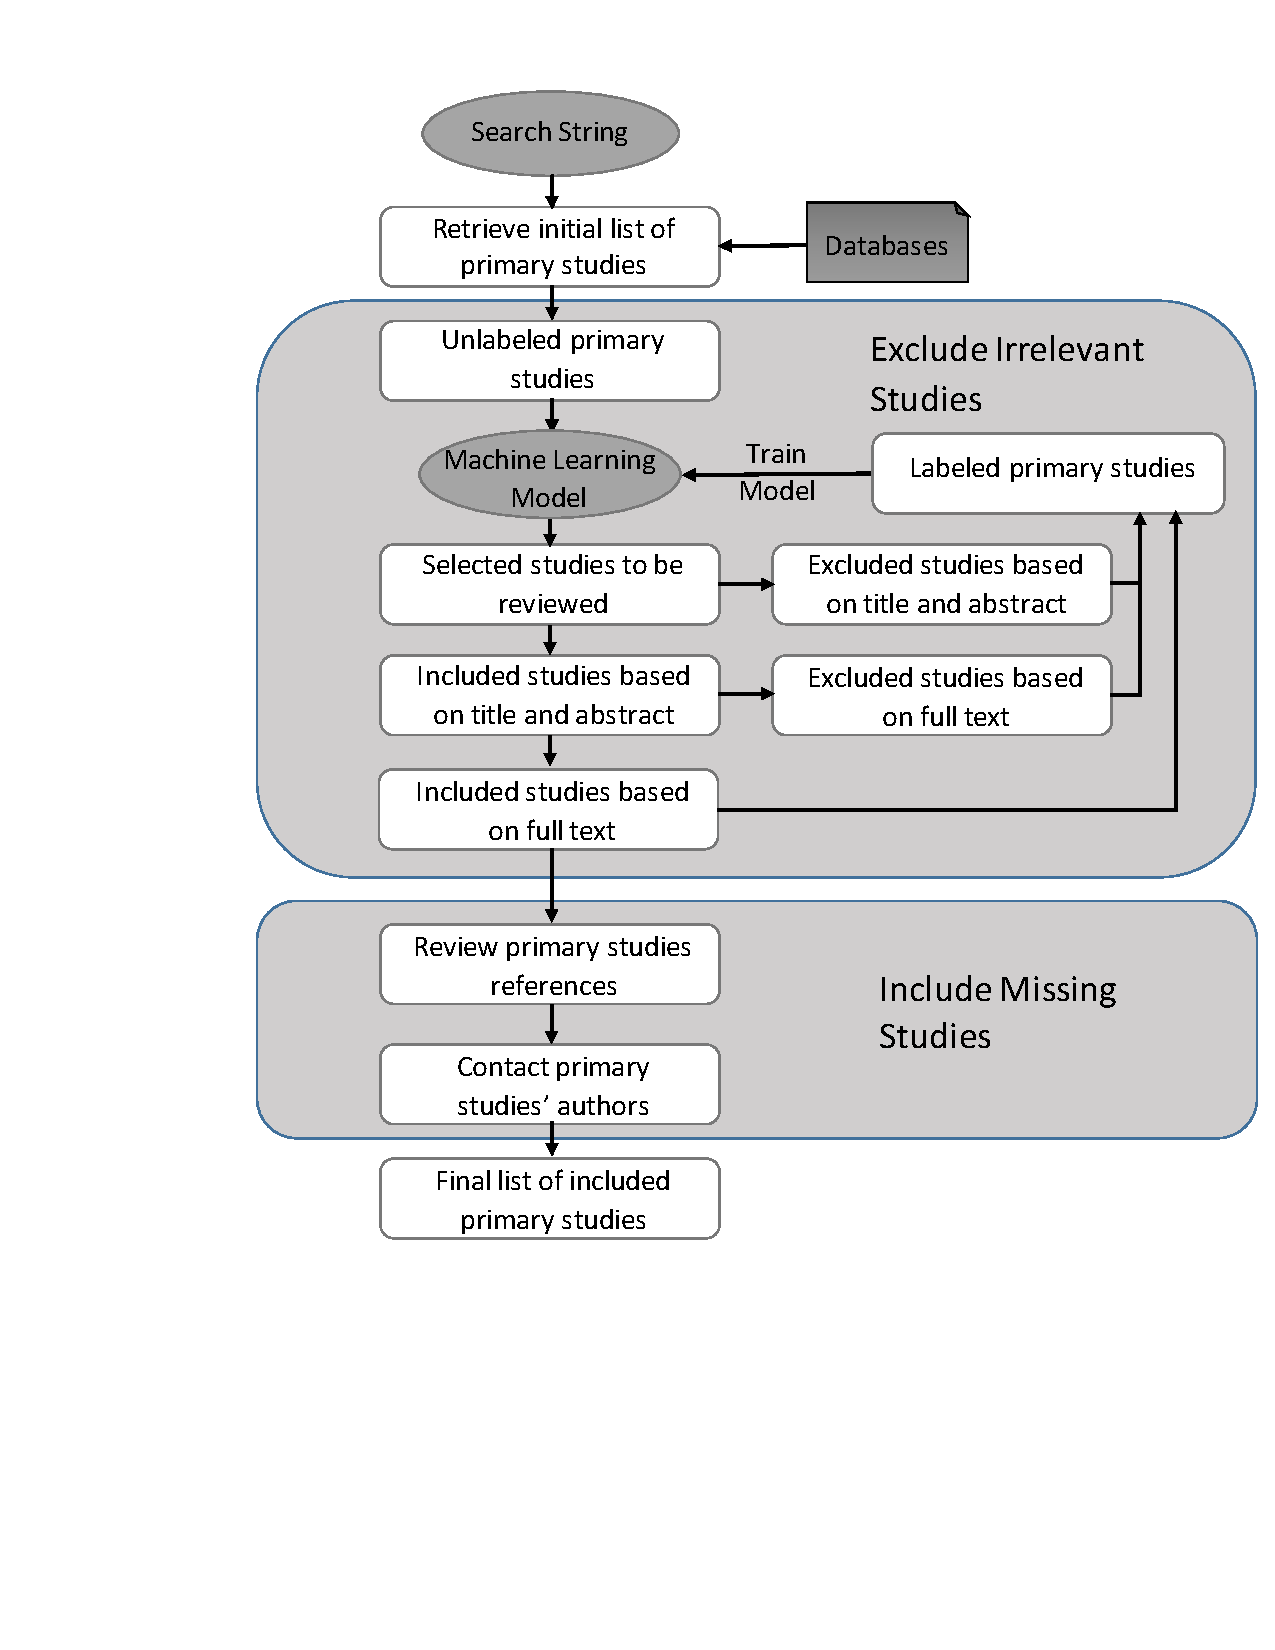
\includegraphics[width=0.6\linewidth]{Learning_based_primary_study_selection.pdf}
    \caption{Human-in-the-loop Primary study selection.}
    \label{fig: learning}
\end{figure}

\subsection{Human-in-the-loop Primary Study Selection}
\label{subsect: Learning based Primary Study Selection}


In contrast to the classical primary study procedures in Fig.~\ref{fig: prime}, with active learning as part of the process, the general form of human-in-the-loop primary study selection is presented in
Fig.~\ref{fig: learning}. Reviewers first review the title and abstract of the
suggested study, determine whether it is ``abstract relevant'' or ``abstract irrelevant''. If the study is relevant by title and abstract, the reviewer will then read the full text of the study and make the final decision-- ``content relevant'' or ``content irrelevant''. In the meantime, all the reviewed
studies will go into the training set. Note that only the title and abstract of the training set studies will be used to train the active learning model, thus making data extraction for training examples easy. Note that in this process, two-level relevance labels are generated and should be available to the active learning model. However, the fact is, for most of our datasets, ``abstract relevant'' labels are missing since they are not reported in the original SLR literature. As a result, only ``content relevant'' labels are being used for training in our experiments. In the rest of the paper, when we say ``relevant'', it means ``content relevant'' while ``irrelevant'' studies include every study that is not ``content relevant'' (``abstract relevant'' but ``content irrelevant'' or ``abstract irrelevant'').

The objective of Human-in-the-loop primary study selection (or machine learning
assisted citation screening or TAR) is different from that of common active
learning scenarios. Instead of trying to build a classifier as good as possible,
human-in-the-loop primary study selection seeks methods to retrieve most
``relevant'' studies with candidate studies reviewed as few as possible. This
difference in the objective leads to a different performance metrics (further explained in Section~\ref{subsect: Performance Metrics}) and thus
makes conventional active learning methods being outperformed by specially
designed methods like PAL~\cite{wallace2010semi}, Certainty plus Weighting~\cite{miwa2014reducing} in evidence-based
medicine and CAL~\cite{cormack2014evaluation,cormack2015autonomy} in
e-discovery.



\subsection{Algorithm Code}
\label{sect: Algorithm Code}

Differences of the three state-of-the-art active learning techniques for systematic reviews are from four aspects: 1) when to start training; 2) query strategy; 3) whether to stop training; 4) data balancing.

\begin{itemize}

\item
{\bf When to start training}: 

\textbf{P} stands for ``patient''. As suggested by Wallace et al.~\cite{wallace2010semi}, ``hasty generation'', which means start training with too few relevant examples, may leads to deteriorate performance. The algorithm keeps random sampling until a sufficient number of ``relevant'' studies retrieved. In our experiments, the sufficient number of ``relevant'' studies retrieved is set to $5$, which means when at least $5$ ``relevant'' studies have been retrieved by random sampling, the algorithm goes into next stage. PAL~\cite{wallace2010semi} and Certainty plus Weighting~\cite{miwa2014reducing} use \textbf{$P$} for when to start training.

\textbf{H} is the opposite. The algorithm stops random sampling as long as {\em ONE} ``relevant'' studies are retrieved, as suggested in CAL~\cite{cormack2014evaluation,cormack2015autonomy}.

\item
{\bf Query strategy}: 

\textbf{U} stands for ``uncertainty sampling''. The algorithm utilizes
uncertainty sampling to build the classifier, where unlabeled examples closest to the SVM decision plane are sampled for query. PAL~\cite{wallace2010semi} uses \textbf{U} for Query strategy.

\textbf{C} stands for ``certainty sampling''. The algorithm utilizes certainty sampling to build the classifier, where unlabeled examples furthest to the SVM decision plane and lie in the ``relevant'' side are sampled for query. Certainty plus Weighting~\cite{miwa2014reducing} and CAL~\cite{cormack2014evaluation,cormack2015autonomy} use \textbf{C} for query strategy.

\item
{\bf Whether to stop training}: 

\textbf{S} stands for ``stop training''. The algorithm stops training
once the classifier is stable. In our experiments, the classifier is treated as stable once more than $30$ ``relevant'' studies have been retrieved as training examples. PAL~\cite{wallace2010semi} uses \textbf{$S$} for whether to stop training.

\textbf{T} stands for ``continue training''. The algorithm never stops
training as suggested in CAL~\cite{cormack2014evaluation,cormack2015autonomy} and Certainty plus Weighting~\cite{miwa2014reducing}. If query strategy is \textbf{U}, algorithm switches to certainty sampling after classifier is stable but training never stops.

\item
{\bf Data balancing}: 

\textbf{N} stands for ``no data balancing''. The algorithm does not balance the training data as suggested by CAL~\cite{cormack2014evaluation,cormack2015autonomy}.

\textbf{A} stands for ``aggressive undersampling''. The algorithm utilizes aggressive undersampling when classifier is stable, as suggested by PAL~\cite{wallace2010semi}.

\textbf{W} stands for ``Weighting''. The algorithm utilizes Weighting for data balancing (before and after the classifier is stable), as suggested by Certainty plus Weighting~\cite{miwa2014reducing}.

\textbf{M} stands for ``mixing of Weighting and aggressive undersampling''. Weighting is applied before the classifier is stable while aggressive undersampling is applied after the classifier is stable. This treatment comes from the observation that ``Weighting'' performs good in early stages while ``aggressive undersampling'' performs good in late stages.

\end{itemize}
As a result, we ended up with 32 treatments including the state-of-the-art treatments as
\begin{itemize}
\item
\textbf{PUSA}: patient active learning~\cite{wallace2010semi,wallace2010active};
\item
\textbf{PCTW}: Certainty plus Weighting~\cite{miwa2014reducing};
\item
\textbf{HCTN}: continuous active learning~\cite{cormack2014evaluation,cormack2015autonomy}. 
\end{itemize}
All the 32 algorithms are tested and compared in Section~\ref{sect: Experiments}.

\section{Experiments}
\label{sect: Experiments}

This section describes the experimental procedures that we used to evaluate the treatments described in Section~\ref{sect: Algorithm Code} on the datasets described in Section~\ref{sect: datasets}. 

There is no human activity involved in these experiments, when asked for a label, the true label in the dataset is queried instead of a human reviewer. As a result, each experiment can be repeated with different random seed to capture variances and also makes reproducing the experiments possible. Each experiment is a simulation of one specific treatment on one dataset:

\begin{enumerate}
\item
Starts with an unlabeled collection of candidate studies, e.g. 8911 in Hall as shown in Table~\ref{tab: number}.

\item
\label{select}
Train a model on current labeled examples if enough labeled examples are available.

\item
Select $N=10$ studies based on the prediction of machine learning model on unlabeled examples for review. If no model is trained yet, random sample $N=10$ unlabeled studies.

\item
Query the true labels of the selected studies, i.e. 106 ``relevant'' and 8805 ``irrelevant'' in Hall as shown in Table~\ref{tab: number}, label them as their true labels.

\item
Go back to \ref{select} until finished.

\end{enumerate}


\subsection{Controlled Variables}
\label{subsect: Controlled Variables}

For the sake of a fair comparison, different treatments in Section~\ref{sect: Algorithm Code} share an identical set of controlled variables including preprocessing, featurization and classifier. 

\subsubsection{Preprocessing and Featurization}

Each candidate study in the initial list is first tokenized by stop words removal after concatenating its title and abstract. After tokenization, the bag of words are featurized into a term frequency vector. Then, reduce the dimensionality of the term frequency vector with to keep only $M=4000$ of the terms with highest tf-idf\footnote{For term $t$ in document $d$, $Tfidf(t, d)=w^t_d\times (\log \frac{|D|}{\sum_{d\in D} sgn(w^t_d)}+1)$ where $w^t_i$ is the term frequency of term $t$ in document $d$. For term $t$, $Tfidf(t) = \sum_{d\in D} Tfidf(t,d) = \sum_{d\in D} w^t_d \times (\log \frac{|D|}{\sum_{d\in D} sgn(w^t_d)}+1)$ and is used for feature selection.} score and normalize the hashed matrix by its L2 norm each row at last. TfidfVectorizer in scikit-learn is utilized for the above preprocessing and featurization steps. Alternatives such as stemming, LDA~\cite{blei2003latent}, paragraph vectors~\cite{le2014distributed} require exploration and are scheduled in our future works. 


\subsubsection{Classifier}

For this work we use a linear SVM as the classifier.
SVMs learn a hyperplane that separate relevant from irrelevant examples
in the training data. Linear SVMs do not make complicated assumptions about the data space and so are known to scale to very large, high-dimensional problems~\cite{joachims2006training}. Such linear SVMs are widely used in the state-of-the-art solutions~\cite{miwa2014reducing,cormack2015autonomy,wallace2010semi}. SVM's hyperplane is a natural tool for deciding what examples to show next to the human user. As discussed in Section~\ref{sect: Technical Briefing}, uncertainty sampling prefers the examples {\em closest} to the hyperplane boundary since these are the ones whose classification will
change, given small changes to the test data. On the other hand, certainty sampling prefers the examples with {\em highest} SVM predictions of being positive. SVC (set to be linear kernel) with default parameters in scikit-learn is utilized as the classifier.


\subsection{Performance Metrics}
\label{subsect: Performance Metrics}

Common active learning aims for building a better model with less training. Therefore, its performance metrics is usually some \textbf{accuracy, precision, recall} on the model prediction vs \textbf{training size} curve. The \textbf{accuracy, precision, recall} are measured on some validation set.

On the other hand, since the goal of human-in-the-loop primary study selection described in Section~\ref{subsect: Learning based Primary Study Selection} is different from that of common active learning, the performance metrics is also different. In human-in-the-loop primary study selection, the performance of each algorithm is evaluated by its \textbf{recall} vs. \textbf{studies reviewed} curve. The \textbf{recall} here is not a measurement on the trained model, but the number of ``relevant'' studies retrieved over the total number of ``relevant'' studies. An algorithm is better than the other if it can retrieve more ``relevant'' studies with fewer studies reviewed. This performance metrics is suggested by~\cite{cormack2015autonomy,cormack2014evaluation,tredennick2015} and best fits the objective of human-in-the-loop primary study selection. To enable a statistical analysis of the performances, the \textbf{recall} vs. \textbf{studies reviewed} curve is cut by a $0.95$ \textbf{recall} line and \textbf{studies reviewed} when reaching $0.95$ \textbf{recall} is used to assess performances. The reason behind $0.95$ \textbf{recall} is that a) $1.00$ \textbf{recall} can never be guaranteed by any text mining method unless all the candidate studies are reviewed; b) $0.95$ \textbf{recall} is usually considered acceptable in evidence-based medicine~\cite{cohen2011performance,cohen2006reducing,o2015using} despite the fact that there might still be ``relevant'' studies missing~\cite{shemilt2016use}. As a result, two numbers are recorded during experiments:
\begin{itemize}
\item
X95 = $\min \{x | r(x)\geq0.95 R\}$
\item
WSS@95 = $0.95-\text{X95}/T$
\end{itemize}
where in a total number of $T$ candidate studies, $R$ of them are ``relevant'' according to true labels, and $r(x)$ is the number of ``relevant'' studies found when $x$ studies have been reviewed.

Each treatment on each dataset is tested for 30 repeats\footnote{It is suggested that usually a sampling size of $30$ is adequate~\cite{isotalo2001basics}.} with random seeds ranging from 0 to 29. The 30 records collected for each treatment on each dataset are then used for comparison through Scott-Knott analysis as recommended by Mittas \& Angelis in their 2013 IEEE TSE paper~\cite{mittas2013ranking}. Scott-Knott clusters methods with little difference in performance together and rank each cluster with the median performances~\cite{scott1974cluster}. Since the 30 records for each treatment on each dataset do not follow a normal distribution, we utilize nonparametric hypothesis tests. Scott-Knott decides two methods are not of little difference if both bootstrapping~\cite{efron1982jackknife} and an effect size test~\cite{cliff1993dominance} agreed that the difference is statistically significant ($99\%$
confidence) and not a “negligible” effect (Cliff's Delta $\ge$ 0.147).





\subsection{Results}
\label{subsect: Results}


\begin{table*}
\caption{Scott-Knott analysis for number of studies reviewed/ work saved over sampling to reach $95\%$ recall}
\label{tab: scottknott}


\begin{center}
\parbox{.49\linewidth}{
\centering
{\scriptsize \begin{tabular}{l@{~~~}l@{~~~}r@{~~~}r@{~~~}r@{~~~}r}
\arrayrulecolor{lightgray}
\multicolumn{2}{l}{\textbf{Wahono}}  & \multicolumn{2}{c}{\textbf{X95}} & \multicolumn{2}{c}{\textbf{WSS@95}}\\\hline
\textbf{Rank} & \textbf{Treatment} & \textbf{Median} & \textbf{IQR} & \textbf{Median} & \textbf{IQR} \\\hline
\rowcolor{green!40}
  1 &         HUTM &    670  &  230 & 0.85 & 0.04 \\
  1 &         HCTM &    740  &  220 & 0.84 & 0.03 \\
\hline  2 &         HUTA &    780  &  140 & 0.84 & 0.02 \\
  2 &         HCTW &    790  &  90 & 0.84 & 0.02 \\
  2 &         HUTW &    800  &  110 & 0.84 & 0.02 \\
  2 &         HCTA &    800  &  140 & 0.83 & 0.02 \\
\hline  3 &         PCTM &    1150  &  450 & 0.78 & 0.07  \\
  3 &         PUTM &    1180  &  420 & 0.78 & 0.07 \\
  3 &         PCTA &    1190  &  340 & 0.78 & 0.05 \\
  3 &         PUTA &    1190  &  340 & 0.78 & 0.05 \\
\rowcolor{red!30}
  3 &         PCTW &    1210  &  350 &  0.78 & 0.06 \\
  3 &         PUTW &    1220  &  370 &  0.77 & 0.06 \\
\hline  4 &         HUSM &    1410  &  400 & 0.75 & 0.06 \\
\hline  5 &         HUSA &    1610  &  370 & 0.72 & 0.07 \\
\hline  6 &         PUSM &    1810  &  370 & 0.69 & 0.06 \\
\rowcolor{red!30}
  6 &         PUSA &    1910  &  700 & 0.67 & 0.10 \\
\hline  7 &         HUSW &    2220  &  400 & 0.63 & 0.06 \\
  7 &         PUSW &    2240  &  360 & 0.63 & 0.06 \\
\hline  8 &         HUTN &    2700  &  40 & 0.56 & 0.01 \\
\rowcolor{red!30}
  8 &         HCTN &    2720  &  40 & 0.56 & 0.01 \\
  8 &         PCSW &    2860  &  1320 & 0.54 & 0.20 \\
  8 &         PCSM &    2860  &  1320 & 0.54 & 0.20 \\
  8 &         PCTN &    2850  &  1130 & 0.54 & 0.17 \\
  8 &         PUTN &    2850  &  1130 & 0.54 & 0.17 \\
\hline  9 &         PCSN &    3020  &  1810 & 0.51 & 0.26 \\
  9 &         PCSA &    3020  &  1810 & 0.51 & 0.26 \\
\hline 10 &         HUSN &    4320  &  110 &  0.33 & 0.03 \\
 10 &         PUSN &    4370  &  1290 & 0.32 & 0.19 \\
 \rowcolor{blue!50}
\hline 11 &       linear &    6650  &  0 & 0 & 0 \\
 11 &         HCSA &    6490  &  2760 & -0.01 & 0.39 \\
 11 &         HCSN &    6490  &  2760 & -0.01 & 0.39 \\
 11 &         HCSM &    6490  &  3110 & -0.01 & 0.44 \\
 11 &         HCSW &    6490  &  3110 & -0.01 & 0.44 \\
\hline \end{tabular}}
}
\parbox{.49\linewidth}{
\centering
{\scriptsize \begin{tabular}{l@{~~~}l@{~~~}r@{~~~}r@{~~~}r@{~~~}r}
\arrayrulecolor{lightgray}
\multicolumn{2}{l}{\textbf{Hall}}  & \multicolumn{2}{c}{\textbf{X95}} & \multicolumn{2}{c}{\textbf{WSS@95}}\\\hline
\textbf{Rank} & \textbf{Treatment} & \textbf{Median} & \textbf{IQR} & \textbf{Median} & \textbf{IQR} \\\hline
  1 &         HUTW &    350  &  80 & 0.91 & 0.01 \\
  1 &         HUTA &    360  &  140 & 0.91 & 0.02 \\
  \rowcolor{green!40}
  1 &         HUTM &    360  &  140 & 0.91 & 0.02 \\
  1 &         HCTW &    370  &  50 & 0.91 & 0.01 \\
\hline  2 &         HCTM &    400  &  90 & 0.90 & 0.01 \\
  2 &         HCTA &    410  &  140 & 0.90 & 0.02 \\
  2 &         HUTN &    430  &  100 & 0.90 & 0.01 \\
  \rowcolor{red!30}
  2 &         HCTN &    460  &  70 & 0.90 & 0.01 \\
\hline  3 &         HUSM &    630  &  160 & 0.88 & 0.03 \\
\rowcolor{red!30}
  3 &         PCTW &    640  &  190 & 0.88 & 0.02 \\
  3 &         PUTW &    640  &  220 & 0.88 & 0.03 \\
\hline  4 &         PCTN &    680  &  210 & 0.87 & 0.03 \\
  4 &         PUTN &    680  &  200 & 0.87 & 0.03 \\
  4 &         PUTM &    690  &  230 & 0.87 & 0.03 \\
  4 &         PCTA &    730  &  260 & 0.87 & 0.03 \\
  4 &         PCTM &    720  &  230 & 0.87 & 0.03 \\
  4 &         PUTA &    730  &  230 & 0.87 & 0.03 \\
\hline  5 &         HUSW &    790  &  320 & 0.86 & 0.04 \\
  5 &         HUSA &    790  &  200 & 0.86 & 0.03 \\
  5 &         PUSW &    840  &  280 & 0.86 & 0.03 \\
  5 &         PUSM &    860  &  320 & 0.85 & 0.04 \\
  \rowcolor{red!30}
  5 &         PUSA &    970  &  310 & 0.84 & 0.04 \\
\hline  6 &         PCSW &    1560  &  580 & 0.77 & 0.07 \\
  6 &         PCSM &    1560  &  580 & 0.77 & 0.07 \\
\hline  7 &         PUSN &    1680  &  1390 & 0.76 & 0.18 \\
  7 &         PCSN &    1990  &  690 & 0.72 & 0.09 \\
  7 &         PCSA &    1990  &  690 & 0.72 & 0.09 \\
\hline  8 &         HUSN &    2270  &  1230 & 0.69 & 0.16 \\
\hline  9 &         HCSA &    7500  &  5170 & 0.03 & 0.58 \\
  9 &         HCSN &    7500  &  5170 & 0.03 & 0.58 \\
   \rowcolor{blue!50}
  9 &       linear &    8464  &  0 & 0 & 0 \\
  9 &         HCSM &    8840  &  5340 & -0.04 & 0.60 \\
  9 &         HCSW &    8840  &  5340 & -0.04 & 0.60 \\
\hline \end{tabular}}
}


\parbox{.49\linewidth}{
\centering
{\scriptsize \begin{tabular}{l@{~~~}l@{~~~}r@{~~~}r@{~~~}r@{~~~}r}
\arrayrulecolor{lightgray}
\multicolumn{2}{l}{\textbf{Radjenovi{\'c}}}  & \multicolumn{2}{c}{\textbf{X95}} & \multicolumn{2}{c}{\textbf{WSS@95}}\\\hline
\textbf{Rank} & \textbf{Treatment} & \textbf{Median} & \textbf{IQR} & \textbf{Median} & \textbf{IQR} \\\hline
\rowcolor{green!40}
  1 &         HUTM &    680   &  180  & 0.83 & 0.03 \\
  1 &         HCTM &    780   &  130  & 0.82 & 0.02 \\
  1 &         HCTA &    790   &  180  & 0.82 & 0.03 \\
  1 &         HUTA &    800   &  180  & 0.82 & 0.03 \\
\hline  2 &         HUSA &    890   &  310  & 0.80 & 0.06 \\
  2 &         HUSM &    890   &  270  & 0.80 & 0.05 \\
\hline  3 &         HUTW &    960   &  80  & 0.79 & 0.02 \\
  3 &         HCTW &    980   &  60  & 0.79 & 0.01 \\
  3 &         HUSW &    1080   &  410  & 0.77 & 0.07 \\
\hline  4 &         PCTM &    1150   &  270  & 0.76 & 0.05 \\
  4 &         PUTM &    1150   &  270  & 0.76 & 0.05 \\
\hline  5 &         HUTN &    1250   &  100  &  0.74 & 0.02 \\
  5 &         PCTA &    1260   &  210  & 0.74 & 0.05 \\
  5 &         PUTA &    1260   &  210  & 0.74 & 0.05 \\
  \rowcolor{red!30}
  5 &         HCTN &    1270   &  70  & 0.74 & 0.02 \\
  5 &         PUSM &    1250   &  400  & 0.74 & 0.07 \\
  5 &         PUSW &    1250   &  450  & 0.73 & 0.08 \\
  5 &         PUTW &    1350   &  310  & 0.72 & 0.06 \\
\rowcolor{red!30}
  5 &         PCTW &    1370   &  310  & 0.72 & 0.06 \\
  \rowcolor{red!30}
  5 &         PUSA &    1400   &  490  & 0.71 & 0.09 \\
\hline  6 &         HUSN &    1570   &  300  & 0.69 & 0.05 \\
  6 &         PCTN &    1600   &  360  & 0.68 & 0.06 \\
  6 &         PUTN &    1600   &  360  & 0.68 & 0.06 \\
\hline  7 &         PUSN &    1890   &  320  &  0.64 & 0.06 \\
\hline
  8 &         PCSW &    2250   &  940  & 0.57 & 0.20 \\
  8 &         PCSM &    2250   &  940  & 0.57 & 0.20 \\
\hline  9 &         PCSN &    2840   &  1680  & 0.47 & 0.31 \\
  9 &         PCSA &    2840   &  1680  & 0.47 & 0.31 \\
\hline 10 &         HCSA &    5310   &  2140  & 0.07 & 0.36 \\
 10 &         HCSN &    5310   &  2140  & 0.07 & 0.36  \\
 10 &         HCSM &    5320   &  2200  &  0.02 & 0.37  \\
 10 &         HCSW &    5320   &  2200  & 0.02 & 0.37 \\
 \rowcolor{blue!50}
 10 &       linear &    5700   &  0  & 0 & 0 \\
\hline \end{tabular}}}
\parbox{.49\linewidth}{
\centering
{\scriptsize \begin{tabular}{l@{~~~}l@{~~~}r@{~~~}r@{~~~}r@{~~~}r}
\arrayrulecolor{lightgray}
\multicolumn{2}{l}{\textbf{Kitchenham}}  & \multicolumn{2}{c}{\textbf{X95}} & \multicolumn{2}{c}{\textbf{WSS@95}}\\\hline
\textbf{Rank} & \textbf{Treatment} & \textbf{Median} & \textbf{IQR} & \textbf{Median} & \textbf{IQR} \\\hline
\rowcolor{green!40}
  1 &         HUTM &    760  &  170 & 0.50 & 0.14 \\
  1 &         HUTA &    840  &  100 & 0.46 & 0.06 \\
  1 &         PUTM &    850  &  180 & 0.45 & 0.11 \\
  1 &         PCTM &    860  &  130 & 0.44 & 0.09 \\
\hline  2 &         HCTA &    900  &  190 & 0.42 & 0.14 \\
  2 &         PCTA &    930  &  170 & 0.40 & 0.11 \\
  2 &         HCTM &    930  &  130 & 0.40 & 0.08 \\
  2 &         PUTA &    930  &  170 & 0.40 & 0.11 \\
\hline  3 &         PUSW &    1140  &  250 & 0.27 & 0.15 \\
  3 &         PUSM &    1140  &  250 & 0.27 & 0.15 \\
  3 &         HUTW &    1160  &  10 & 0.27 & 0.01 \\
  3 &         HCTW &    1180  &  40 & 0.25 & 0.03 \\
  \rowcolor{red!30}
  3 &         PCTW &    1190  &  170 & 0.25 & 0.10 \\
  3 &         PUTW &    1190  &  170 & 0.25 & 0.10 \\
\hline  4 &         HUSW &    1200  &  150 & 0.24 & 0.10 \\
  4 &         HUSM &    1200  &  150 & 0.24 & 0.10 \\
  4 &         HUSN &    1250  &  220 & 0.21 & 0.14 \\
  4 &         HUSA &    1250  &  220 & 0.21 & 0.14 \\
  \rowcolor{red!30}
  4 &         PUSA &    1250  &  290 & 0.21 & 0.19 \\
  4 &         PUSN &    1250  &  290 & 0.21 & 0.19 \\
  4 &         HUTN &    1260  &  10 & 0.21 & 0.01 \\
  \rowcolor{red!30}
  4 &         HCTN &    1280  &  30 & 0.20 & 0.02 \\
  4 &         PUTN &    1280  &  260 & 0.19 & 0.16 \\
  4 &         PCTN &    1290  &  260 & 0.19 & 0.15 \\
\hline  5 &         PCSW &    1370  &  260 & 0.14 & 0.22 \\
  5 &         PCSM &    1370  &  260 & 0.14 & 0.22 \\
  5 &         PCSN &    1400  &  340 & 0.12 & 0.22 \\
  5 &         PCSA &    1400  &  340 & 0.12 & 0.22 \\
\rowcolor{blue!50}
\hline  6 &       linear &    1615  &  0 & 0 & 0 \\
\hline  7 &         HCSA &    1670  &  90 & -0.03 & 0.05 \\
  7 &         HCSN &    1670  &  90 & -0.03 & 0.05 \\
  7 &         HCSM &    1670  &  90 & -0.03 & 0.05 \\
  7 &         HCSW &    1670  &  90 & -0.03 & 0.05 \\
\hline \end{tabular}}}

\end{center}
{\footnotesize Simulations are repeated for $30$ times, medians ($50$th percentile) and iqrs (($75$-$25$)th percentile) are presented. Smaller/larger median value for X90/WSS@95 represents better performance while smaller iqr means better stability. Treatments with same rank have no significant difference in performance while treatments of smaller number in rank are significantly better than those of larger number in rank. The recommended treatment FASTREAD is colored in {\setlength{\fboxsep}{1pt}\colorbox{green!40}{green}} while the state-of-the-art treatments are colored in {\setlength{\fboxsep}{1pt}\colorbox{red!30}{red}} and linear review is colored in {\setlength{\fboxsep}{1pt}\colorbox{blue!50}{blue}}.}


\end{table*}



\begin{table*}
\caption{Experimental results rearranged as blocks to compare the effectiveness of each code}
\label{tab: blockings}
\begin{center}
\parbox{.49\linewidth}{
\centering
\subfloat[64 blocks for RQ2.1 (T/S)]{
\label{tab: TS}
{\scriptsize \begin{tabular}{l@{~~~}|c@{~~~}c@{~~~}c@{~~~}c}
\arrayrulecolor{lightgray}
\textbf{T/S} & \multicolumn{4}{c}{\textbf{Scott-Knott Rank}} \\\hline
\textbf{Treatment} & \textbf{Wahono} & \textbf{Hall} & \textbf{Radjenovi{\'c}} & \textbf{Kitchenham} \\\hline
HUTM & \cellcolor{green!40} 1 & \cellcolor{green!40}1 & \cellcolor{green!40}1 & \cellcolor{green!40}1\\
HUSM & 4 & 3 & 2 & 4\\
\hline
HUTA &\cellcolor{green!40} 2 &\cellcolor{green!40} 1 &\cellcolor{green!40} 1 &\cellcolor{green!40} 1\\
HUSA & 5 & 5 & 2 & 4\\
\hline
HUTW &\cellcolor{green!40} 2 &\cellcolor{green!40} 1 & 3 &\cellcolor{green!40} 3\\
HUSW & 7 & 5 & 3 & 4\\
\hline
HUTN &\cellcolor{green!40} 8 &\cellcolor{green!40} 2 &\cellcolor{green!40} 5 & 4\\
HUSN & 10 & 8 & 6 & 4\\
\hline
HCTM &\cellcolor{green!40} 1 &\cellcolor{green!40} 2 &\cellcolor{green!40} 1 &\cellcolor{green!40} 2\\
HCSM & 11 & 9 & 10 & 7\\
\hline
HCTA &\cellcolor{green!40} 2 &\cellcolor{green!40} 2 &\cellcolor{green!40} 1 &\cellcolor{green!40} 2\\
HCSA & 11 & 9 & 10 & 7\\
\hline
HCTW &\cellcolor{green!40} 2 &\cellcolor{green!40} 1 &\cellcolor{green!40} 3 &\cellcolor{green!40} 3\\
HCSW & 11 & 9 & 10 & 7\\
\hline
HCTN &\cellcolor{green!40} 8 &\cellcolor{green!40} 2 &\cellcolor{green!40} 5 &\cellcolor{green!40} 4\\
HCSN & 11 & 9 & 10 & 7\\
\hline
PUTM &\cellcolor{green!40} 3 &\cellcolor{green!40} 4 &\cellcolor{green!40} 4 &\cellcolor{green!40} 1\\
PUSM & 6 & 5 & 5 & 3\\
\hline
PUTA &\cellcolor{green!40} 3 &\cellcolor{green!40} 4 & 5 & \cellcolor{green!40}2\\
PUSA & 6 & 5 & 5 & 4\\
\hline
PUTW &\cellcolor{green!40} 3 & \cellcolor{green!40}3 & 5 & 3\\
PUSW & 7 & 5 & 5 & 3\\
\hline
PUTN & \cellcolor{green!40}8 &\cellcolor{green!40} 4 &\cellcolor{green!40} 6 & 4\\
PUSN & 10 & 7 & 7 & 4\\
\hline
PCTM & \cellcolor{green!40}3 &\cellcolor{green!40} 4 &\cellcolor{green!40} 4 &\cellcolor{green!40} 1\\
PCSM & 8 & 6 & 8 & 5\\
\hline
PCTA & \cellcolor{green!40}3 &\cellcolor{green!40} 4 & \cellcolor{green!40}5 &\cellcolor{green!40} 2\\
PCSA & 9 & 7 & 9 & 5\\
\hline
PCTW & \cellcolor{green!40}3 &\cellcolor{green!40} 3 &\cellcolor{green!40} 5 &\cellcolor{green!40} 3\\
PCSW & 8 & 6 & 8 & 5\\
\hline
PCTN & \cellcolor{green!40}8 &\cellcolor{green!40} 4 & \cellcolor{green!40}6 & \cellcolor{green!40}4\\
PCSN & 9 & 7 & 9 & 5\\
\hline
\end{tabular}}
}}
\parbox{.49\linewidth}{
\centering
\subfloat[64 blocks for RQ2.2 (U/C)]{
\label{tab: UC}
{\scriptsize \begin{tabular}{l@{~~~}|c@{~~~}c@{~~~}c@{~~~}c}
\arrayrulecolor{lightgray}
\textbf{U/C} & \multicolumn{4}{c}{\textbf{Scott-Knott Rank}} \\\hline
\textbf{Treatment} & \textbf{Wahono} & \textbf{Hall} & \textbf{Radjenovi{\'c}} & \textbf{Kitchenham} \\\hline
HUTM & 1 & \cellcolor{green!40}1 & 1 & \cellcolor{green!40}1\\
HCTM & 1 & 2 & 1 & 2\\
\hline
HUTA & 2 &\cellcolor{green!40} 1 & 1 &\cellcolor{green!40} 1\\
HCTA & 2 & 2 & 1 & 2\\
\hline
HUTW & 2 & 1 & 3 & 3\\
HCTW & 2 & 1 & 3 & 3\\
\hline
HUTN & 8 & 2 & 5 & 4\\
HCTN & 8 & 2 & 5 & 4\\
\hline
HUSM & \cellcolor{green!40}4 &\cellcolor{green!40} 3 & \cellcolor{green!40}2 &\cellcolor{green!40} 4\\
HCSM & 11 & 9 & 10 & 7\\
\hline
HUSA &\cellcolor{green!40} 5 & \cellcolor{green!40}5 & \cellcolor{green!40}2 & \cellcolor{green!40}4\\
HCSA & 11 & 9 & 10 & 7\\
\hline
HUSW & \cellcolor{green!40}7 & \cellcolor{green!40}5 &\cellcolor{green!40} 3 &\cellcolor{green!40} 4\\
HCSW & 11 & 9 & 10 & 7\\
\hline
HUSN &\cellcolor{green!40} 10 &\cellcolor{green!40} 8 &\cellcolor{green!40} 6 &\cellcolor{green!40} 4\\
HCSN & 11 & 9 & 10 & 7\\
\hline
PUTM & 3 & 4 & 4 & 1\\
PCTM & 3 & 4 & 4 & 1\\
\hline
PUTA & 3 & 4 & 5 & 2\\
PCTA & 3 & 4 & 5 & 2\\
\hline
PUTW & 3 & 3 & 5 & 3\\
PCTW & 3 & 3 & 5 & 3\\
\hline
PUTN & 8 & 4 & 6 & 4\\
PCTN & 8 & 4 & 6 & 4\\
\hline
PUSM & \cellcolor{green!40}6 & \cellcolor{green!40}5 &\cellcolor{green!40} 5 &\cellcolor{green!40} 3\\
PCSM & 8 & 6 & 8 & 5\\
\hline
PUSA &\cellcolor{green!40} 6 &\cellcolor{green!40} 5 & \cellcolor{green!40}5 &\cellcolor{green!40} 4\\
PCSA & 9 & 7 & 9 & 5\\
\hline
PUSW &\cellcolor{green!40} 7 &\cellcolor{green!40} 5 &\cellcolor{green!40} 5 &\cellcolor{green!40} 3\\
PCSW & 8 & 6 & 8 & 5\\
\hline
PUSN & \cellcolor{blue!50}10 & 7 & \cellcolor{green!40}7 &\cellcolor{green!40} 4\\
PCSN & 9 & 7 & 9 & 5\\
\hline
\end{tabular}}
}}

\parbox{.49\linewidth}{
\centering
\subfloat[64 blocks for RQ2.3 (H/P)]{
\label{tab: HP}
{\scriptsize \begin{tabular}{l@{~~~}|c@{~~~}c@{~~~}c@{~~~}c}
\arrayrulecolor{lightgray}
\textbf{H/P} & \multicolumn{4}{c}{\textbf{Scott-Knott Rank}} \\\hline
\textbf{Treatment} & \textbf{Wahono} & \textbf{Hall} & \textbf{Radjenovi{\'c}} & \textbf{Kitchenham} \\\hline
HUTM &\cellcolor{green!40} 1 &\cellcolor{green!40} 1 & \cellcolor{green!40}1 & 1\\
PUTM & 3 & 4 & 4 & 1\\
\hline
HUTA &\cellcolor{green!40} 2 &\cellcolor{green!40} 1 &\cellcolor{green!40} 1 &\cellcolor{green!40} 1\\
PUTA & 3 & 4 & 5 & 2\\
\hline
HUTW & \cellcolor{green!40}2 & \cellcolor{green!40}1 &\cellcolor{green!40} 3 & 3\\
PUTW & 3 & 3 & 5 & 3\\
\hline
HUTN & 8 & \cellcolor{green!40}2 & \cellcolor{green!40}5 & 4\\
PUTN & 8 & 4 & 6 & 4\\
\hline
HUSM &\cellcolor{green!40} 4 & \cellcolor{green!40}3 & \cellcolor{green!40}2 &\cellcolor{blue!50} 4\\
PUSM & 6 & 5 & 5 & 3\\
\hline
HUSA &\cellcolor{green!40} 5 & 5 & \cellcolor{green!40}2 & 4\\
PUSA & 6 & 5 & 5 & 4\\
\hline
HUSW & 7 & 5 & \cellcolor{green!40}3 &\cellcolor{blue!50} 4\\
PUSW & 7 & 5 & 5 & 3\\
\hline
HUSN & 10 &\cellcolor{blue!50} 8 &\cellcolor{green!40} 6 & 4\\
PUSN & 10 & 7 & 7 & 4\\
\hline
HCTM &\cellcolor{green!40} 1 &\cellcolor{green!40} 2 &\cellcolor{green!40} 1 & \cellcolor{blue!50}2\\
PCTM & 3 & 4 & 4 & 1\\
\hline
HCTA & \cellcolor{green!40}2 & \cellcolor{green!40}2 &\cellcolor{green!40} 1 & 2\\
PCTA & 3 & 4 & 5 & 2\\
\hline
HCTW &\cellcolor{green!40} 2 & \cellcolor{green!40}1 &\cellcolor{green!40} 3 & 3\\
PCTW & 3 & 3 & 5 & 3\\
\hline
HCTN & 8 &\cellcolor{green!40} 2 & \cellcolor{green!40}5 & 4\\
PCTN & 8 & 4 & 6 & 4\\
\hline
HCSM & \cellcolor{blue!50}11 & \cellcolor{blue!50}9 & \cellcolor{blue!50}10 &\cellcolor{blue!50} 7\\
PCSM & 8 & 6 & 8 & 5\\
\hline
HCSA &\cellcolor{blue!50} 11 &\cellcolor{blue!50} 9 &\cellcolor{blue!50} 10 &\cellcolor{blue!50} 7\\
PCSA & 9 & 7 & 9 & 5\\
\hline
HCSW & \cellcolor{blue!50}11 & \cellcolor{blue!50}9 & \cellcolor{blue!50}10 & \cellcolor{blue!50}7\\
PCSW & 8 & 6 & 8 & 5\\
\hline
HCSN & \cellcolor{blue!50}11 &\cellcolor{blue!50} 9 & \cellcolor{blue!50}10 & \cellcolor{blue!50}7\\
PCSN & 9 & 7 & 9 & 5\\
\hline
\end{tabular}}
}}
\parbox{.49\linewidth}{
\centering
\subfloat[32 blocks for RQ2.4 (M/A/W/N)]{
\label{tab: MAWN}
{\scriptsize \begin{tabular}{l@{~~~}|c@{~~~}c@{~~~}c@{~~~}c}
\arrayrulecolor{lightgray}
\textbf{M/A/W/N} & \multicolumn{4}{c}{\textbf{Scott-Knott Rank}} \\\hline
\textbf{Treatment} & \textbf{Wahono} & \textbf{Hall} & \textbf{Radjenovi{\'c}} & \textbf{Kitchenham} \\\hline
HUTM & \cellcolor{green!40}1 & 1 & 1 & 1\\
HUTA & 2 & 1 & 1 & 1\\
HUTW & 2 & 1 & 3 & 3\\
HUTN & 8 & 2 & 5 & 4\\
\hline
HUSM & \cellcolor{green!40}4 &\cellcolor{green!40} 3 & 2 & 4\\
HUSA & 5 & 5 & 2 & 4\\
HUSW & 7 & 5 & 3 & 4\\
HUSN & 10 & 8 & 6 & 4\\
\hline
HCTM &\cellcolor{green!40} 1 & \cellcolor{blue!50}2 & 1 & 2\\
HCTA & 2 & 2 & 1 & 2\\
HCTW & 2 & 1 & 3 & 3\\
HCTN & 8 & 2 & 5 & 4\\
\hline
HCSM & 11 & 9 & 10 & 7\\
HCSA & 11 & 9 & 10 & 7\\
HCSW & 11 & 9 & 10 & 7\\
HCSN & 11 & 9 & 10 & 7\\
\hline
PUTM & 3 &\cellcolor{blue!50} 4 & \cellcolor{green!40}4 &\cellcolor{green!40} 1\\
PUTA & 3 & 4 & 5 & 2\\
PUTW & 3 & 3 & 5 & 3\\
PUTN & 8 & 4 & 6 & 4\\
\hline
PUSM & 6 & 5 & 5 & 3\\
PUSA & 6 & 5 & 5 & 4\\
PUSW & 7 & 5 & 5 & 3\\
PUSN & 10 & 7 & 7 & 4\\
\hline
PCTM & 3 & \cellcolor{blue!50}4 & \cellcolor{green!40}4 &\cellcolor{green!40} 1\\
PCTA & 3 & 4 & 5 & 2\\
PCTW & 3 & 3 & 5 & 3\\
PCTN & 8 & 4 & 6 & 4\\
\hline
PCSM & 8 & 6 & 8 & 5\\
PCSA & 9 & 7 & 9 & 5\\
PCSW & 8 & 6 & 8 & 5\\
PCSN & 9 & 7 & 9 & 5\\
\hline
\end{tabular}}
}}
\end{center}
{\footnotesize Each subtable compares one pair of algorithm codes by rearranging the results from Table~\ref{tab: scottknott} so that codes other than the ones to be compared with are identical within each block. Smaller number in rank means better performance while same number in rank means no significant difference in performance. All the blocks where the suggested code performs significantly better than its alternatives are colored in {\setlength{\fboxsep}{1pt}\colorbox{green!40}{green}} while all the blocks where the suggested code is outperformed by any other code are colored in {\setlength{\fboxsep}{1pt}\colorbox{blue!50}{blue}}. Results are summarized as following: (a) {\setlength{\fboxsep}{1pt}\colorbox{green!40}{58}}/{\setlength{\fboxsep}{1pt}\colorbox{blue!50}{0}}; (b) {\setlength{\fboxsep}{1pt}\colorbox{green!40}{34}}/{\setlength{\fboxsep}{1pt}\colorbox{blue!50}{1}}; (c) {\setlength{\fboxsep}{1pt}\colorbox{green!40}{30}}/{\setlength{\fboxsep}{1pt}\colorbox{blue!50}{20}}; (d) {\setlength{\fboxsep}{1pt}\colorbox{green!40}{8}/\colorbox{blue!50}{3}}.
}
\end{table*}


{\bf RQ1: Can active learning techniques reduce cost in primary study selection?} 

In Table~\ref{tab: scottknott}, we tested 32 active learning treatments and linear review. According to the results, most active learning treatments perform consistently better than linear review (colored in {\setlength{\fboxsep}{1pt}\colorbox{blue!50}{blue}}) on all four datasets while four treatments (\textbf{HCS*}) can be even worse than linear review. Interestingly these four treatments share same codes of \textbf{HCS}, which hastily start training (\textbf{H}) with greedy query strategy (\textbf{C}) and give up the attempt to correct the model short after (\textbf{S}). The problem of ``hasty generation'' is maximized in the setting of \textbf{HCS} and thus leads to an even worse performance than linear review. In general, other active learning treatments can reduce review costs by allowing the reviewer to read fewer studies while still find 95\% of the relevant ones.

\begin{lesson}
    In general, active learning techniques can reduce cost in primary study selections with a sacrifice of (say 5\%) recall.
\end{lesson}




{\bf RQ2: Should we just adopt the state-of-the-art treatments from other fields? Is it possible to build a better one by mixing and matching from those?}

The performance of the three state-of-the-art treatments are colored in {\setlength{\fboxsep}{1pt}\colorbox{red!30}{red}}. On Wahono and Kitchenham datasets, Certainty plus Weighting (\textbf{PCTW}) outperforms the other two treatments; while on Hall dataset, CAL (\textbf{HCTN}) has the best performance; and on Radjenovi{\'c} dataset, all three treatments perform similarly. PAL (\textbf{PUSA}) seems to be dominated by Certainty plus Weighting (\textbf{PCTW}) but this does not mean techniques in PAL are not useful. In fact, neither of the three state-of-the-art treatments has ever ranked highest (rank 1) in any dataset. This means that adopting the state-of-the-art treatments will not produce best results. According to Scott-Knott analysis, the performance of one treatment, \textbf{HUTM} (colored in {\setlength{\fboxsep}{1pt}\colorbox{green!40}{green}}), consistently stays in the top rank across all four datasets. Before asserting that \textbf{HUTM} is our preferred treatment, let us analyze the effectiveness of each algorithm code.

\textbf{RQ2.1}: Stop training or not?

Table~\ref{tab: TS} rearranges the results such that in each block, only the code for whether to stop training are different (\textbf{T} vs. \textbf{S}). Across the $4\times 16 = 64$ blocks, \textbf{T} (continue training) performs significantly better than \textbf{S} (stop training) in 58 blocks and performs similarly to \textbf{S} in the rest 6 blocks. Therefore, \textbf{T} dominates\footnote{We say Code A dominates Code B if in every block, A performs no worse than B and in some blocks A performs significantly better than B.} \textbf{S}. Although training time can be saved by \textbf{S}, it sacrifices the performance and the ability to adapt. So no, never stop training.

\textbf{RQ2.2}: Which query strategy is more effective?

Table~\ref{tab: UC} rearranges the results so that in each block, only the code for query strategy are different (\textbf{U} vs. \textbf{C}). Across the $4\times 16 = 64$ blocks, \textbf{U} (uncertainty sampling) performs significantly better than \textbf{C} (certainty sampling) in 34 blocks while the other way around in 1 blocks. Overall, \textbf{U} performs better than \textbf{C} and if only considering the $4\times 8 = 32$ \textbf{T} blocks, \textbf{U} dominates \textbf{C}. Therefore, uncertainty sampling is suggested for query strategy in early stages especially if \textbf{T} continue training is applied.

\textbf{RQ2.3}: When to start training?

Table~\ref{tab: HP} rearranges the results so that in each block, only the code for when to start training are different (\textbf{H} vs. \textbf{P}). Across the $4\times 16 = 64$ blocks, \textbf{H} (hasty, start training with 1 ``relevant'' example) performs significantly better than \textbf{P} (patient, start training with at least 5 ``relevant'' examples) in 30 blocks while the other way around in 20 blocks. No clear winners from the overall view. However, if only considering the $4\times 4 = 16$ \textbf{UT} blocks, \textbf{H} dominates \textbf{P}. Therefore, \textbf{H} starting training with 1 ``relevant'' example is suggested if \textbf{U} uncertainty sampling and \textbf{T} continue training are applied.

\textbf{RQ2.4}: Which data balancing method is most effective?

Table~\ref{tab: MAWN} rearranges the results so that in each block, only the code for data balancing are different (\textbf{M}, \textbf{A}, \textbf{W}, or \textbf{N}). Across the $4\times 8 = 32$ blocks, \textbf{M} (Weighting plus aggressive undersampling) performs significantly better than the rest in 8 blocks while \textbf{W} (Weighting) performs significantly better than the rest in 3 blocks. Overall, a) \textbf{N} (no data balancing) is dominated by any data balancing method in every block; b) \textbf{M} dominates other codes on Wahono, Radjenovi{\'c}, and Kitchenham datasets; c) \textbf{W} dominates other codes on Hall datasets; d) across all $4$ blocks of \textbf{HUT}, \textbf{M} dominates other codes. To conclude, data balancing methods are effective; \textbf{M} Weighting plus aggressive undersampling is suggested if \textbf{U} uncertainty sampling and \textbf{T} continue training are applied and \textbf{H} training starts with 1 ``relevant'' example.

As indicated in the answers for \textbf{RQ2.1-2.4}, \textbf{UT} are definitely better than their alternatives while \textbf{H} and \textbf{M} are conditionally better given the selection of other codes. Together, it forms our recommended treatment \textbf{HUTM}, which 
\begin{enumerate}
\item
randomly samples from unlabeled candidate studies until 1 ``relevant'' example retrieved;
\item
then start training with Weighting and query with uncertainty sampling, until 30 ``relevant'' examples retrieved;
\item
then train with aggressive undersampling and query with certainty sampling until finished.
\end{enumerate}

This treatment is named as FASTREAD. According to Table~\ref{tab: scottknott}, FASTREAD (\textbf{HUTM}) consistently shows in the first rank across all four datasets and significantly outperforms all three state-of-the-art treatments.

\begin{lesson}
    No, we should not just adopt the state-of-the-art methods from other fields. A better method called FASTREAD is generated by mixing and matching from the state-of-the-art methods.
\end{lesson}

\begin{table}
\caption{How much can FASTREAD save?}
\label{tab: save}
\begin{center}
\begin{tabular}{ |l|c|c|c|}
  \hline
   Datasets & \# Studies Reviewed & Review Cost & \# Relevant Studies \\
  \hline
  Wahono & $7002-670=6332$ & $\geq6332C_A+4C_D$ & 4\\
  \hline
  Hall & $8991-360=8631$ & $\geq8611C_A+6C_D$ & 6\\
  \hline
  Radjenovi{\'c} & $6000-680=5320$ & $\geq5320C_A+3C_D$ & 3\\
  \hline
  Kitchenham & $1704-760=944$ & $32C_D+944C_A$ & 3\\
  \hline
%   Kitchenham (abstract) & 334 & $6C_D+334C_A$ & -1\\
%   \hline
\end{tabular}
\end{center}
{\footnotesize Numbers of reviewing every candidate study minus numbers of reviewing with FASTREAD. For example, on Kitchenham dataset, FASTREAD reviews 944 fewer studies, which costs $32C_D+944C_A$ less review effort, while misses 3 ``relevant'' ones. Here $C_D$ is the cost to review a study by its content and $C_A$ is the cost to review a study by its title and abstract.}
\end{table}

\textbf{RQ3: How much effort can FASTREAD save in an SLR?}

In terms of the number of studies reviewed, WSS@95 scores in Tabel~\ref{tab: scottknott} reflects how much FASTREAD can save. Number of ``relevant'' studies ($|R|$) and the total number of candidate studies ($|C|$) affect WSS@95 a lot, e.g. WSS@95=0.50 in Kitchenham dataset with $|R|$=44, $|C|$=1704 and WSS@95=0.91 in Hall dataset with $|R|$=106, $|C|$=8911. Even the smallest number of WSS@95=0.50 in Kitchenham dataset is a success in the reduction of number of studies need to be reviewed comparing to the 5\% recall lost.

In terms of the actual review cost,
%FASTREAD
%saves less since the most burdensome part-- reviewing studies by their content can not be reduced much. On Kitchenham dataset, reviewing every candidate study costs $132C_D+1704C_A$ while with FASTREAD, the cost can be reduced to $100C_D+760C_A$. 
Table~\ref{tab: save} shows how much FASTREAD save over reviewing all candidate studies. Suppose $C_D=9C_A$, following the estimation that Shemilt made: 1 minute to screen a title-abstract record, 4 minutes to retrieve a full-text study report, and 5 minutes to screen a full-text study report~\cite{shemilt2016use}. Then the reduction in review cost is $(32C_D+944C_A)/(132C_D+1704C_A) = 42.6\%$\footnote{According to Table~\ref{tab: number}, reviewing all studies costs $132C_D+1704C_A$. In our simulations, in average FASTREAD did 760 abstract reviews and 100 content reviews.}. On other datasets, although we do not have the exact number of ``abstract relevant'' studies, we can estimate the worst case review cost reduction\footnote{In the worst case we assume that every study reviewed is ``abstract relevant'' and thus costs $C_D+C_A$ to review and there is no ``abstract relevant'' study left except for the 5\% missing ``content relevant'' ones. E.g. in Wahono dataset, FASTREAD reviews 670 studies among the 7002 candidate ones, it costs $670(C_A+C_D)$ while reviewing all studies costs $(670+4)C_D+7002C_A$.} with the numbers in Table~\ref{tab: number} and Table~\ref{tab: save}: a) Wahono dataset: $1-670(C_A+C_D)/((670+4)C_D+7002C_A) = 48.7\%$; b) Hall dataset: $1-360(C_A+C_D)/((360+6)C_D+8991C_A) = 70.7\%$; c) Radjenovi{\'c} dataset: $1-680(C_A+C_D)/((680+3)C_D+6000C_A) = 44.0\%$. 
Note that training time costs are negligibly small (1 second for each round in average) compared to the review time $C_A$ because of the small training size (less than 1000 examples before reaching 95\% recall). 
%Utilizing two levels of relevance labels to minimize the review cost is planned in our future works when datasets with the required labels are available.

\begin{lesson}
    Our results and estimations suggest that FASTREAD can save around $40\%$ review cost while retrieving $95\%$ of the ``relevant'' studies.
\end{lesson}

Note that if the reader doubts the value of a 40\% reduction the review cost, they are reminded that that overall cost may be days to weeks to months. Hence, the reductions achieved by FASTREAD are of much practical benefit.





\section{Tool Support}
\label{sect: tool}

\begin{figure*}[!tbhp]
    \centering
    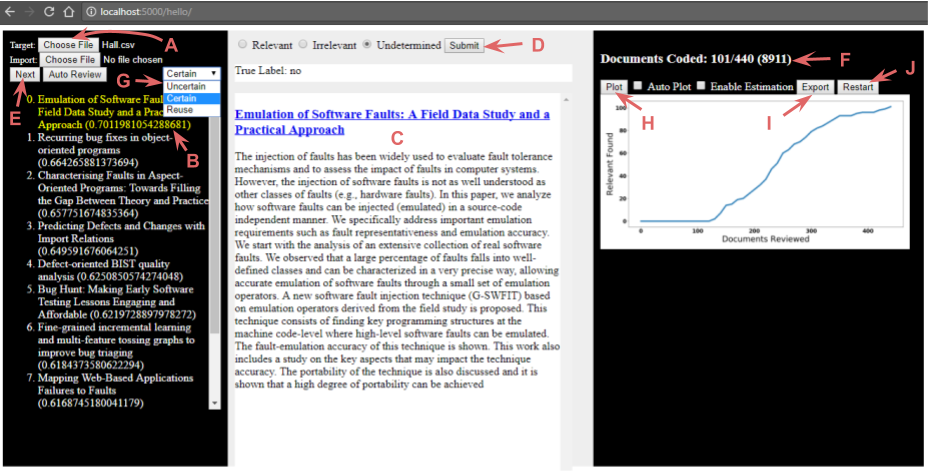
\includegraphics[width=\linewidth]{FASTREAD.png}
    \caption{Basic interface of the FASTREAD tool.}
    \label{fig:FASTREAD}
\end{figure*}


\begin{figure*}[!tbhp]
    \centering
    \subfloat[Input format]
    {
        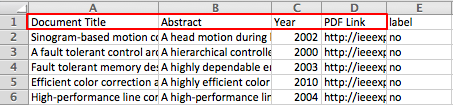
\includegraphics[width=0.48\linewidth]{Input.png}\label{fig:input}
    }
    \subfloat[Output format]
    {
        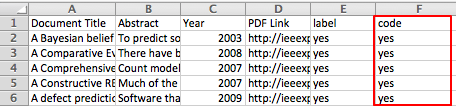
\includegraphics[width=0.48\linewidth]{Output.png}\label{fig:output}
    }    
    
    \caption{Data format for FASTREAD tool.}
    \label{fig:csv}
\end{figure*}

In order to implement FASTREAD, we developed a simple tool as shown in Fig.~\ref{fig:FASTREAD}. This software is freely available from SeaCraft Zenodo at \textit{https://doi.org/10.5281/zenodo.837861} and its Github repository at \textit{https://github.com/fastread/src}. 


Using FASTREAD, a review starts with \textbf{A}: selecting the input candidate study list from \textit{workspace/data/} directory. The input candidate list is specified in the format shown in Fig.~\ref{fig:input}. The input CSV file must have the \textit{Document Title}, \textit{Abstract}, \textit{Year}, and \textit{PDF Link} columns. The \textit{label} column, which is the true label of the candidate studies, is optional and is only used for testing. The output CSV file generated by the FASTREAD tool has an additional \textit{code} column, which is the reviewer-decided label for the candidate study. The final inclusion list can be retrieved by extracting all the studies with ``yes'' in the \textit{code} column.

The review then proceeds as follows:
\begin{enumerate}
\item[\textbf{B}] Randomly select $10$ candidate studies for review.
\item[\textbf{C}] Read through the title and abstract (and click on the title and read the full text if needed) of the candidate study.
\item[\textbf{D}] Decide whether this study should be coded as \textit{Relevant} or \textit{Irrelevant} and click the \textit{Submit} button.
\item[\textbf{E}] Click the \textit{Next} button and the codes are saved. Another $10$ candidate studies will be selected for review.
\item[\textbf{F}] The review status will change every time new studies are coded by reviewer and the \textit{Next} button is hit. The status is shown in the format ``Documents Coded: \textit{Number of relevant studies found} / \textit{Number of studies reviewed} (\textit{Total number of candidate studies}).''
\item[\textbf{G1}] Once \textbf{1} ``relevant'' study is coded, \textit{Random sampling} will be replaced by \textit{Uncertainty sampling}.
\item[\textbf{G2}] Once \textbf{30} ``relevant'' study is coded, \textit{Uncertainty sampling} can be changed to \textit{Certainty sampling}.
\item[\textbf{H}] Fig. can be plotted by clicking the \textit{Plot} button or checking \textit{Auto Plot}. The generated figure can also be found in the \textit{src/static/image/} directory. The new figure will overwrite any old one.
\item[\textbf{I}] Once finished, coded studies can be exported into a CSV file in the \textit{workspace/coded/} directory, in the format shown in Fig.~\ref{fig:output}.
\end{enumerate}

Note that the \textit{Restart} button (\textbf{J}) is only for testing and discards all codes.



\section{Threats to Validity}
\label{sect: Threats to Validity}

There are several validity threats to the design of this study~\cite{feldt2010validity}. Any conclusions made from this work must be considered with the following issues in mind:

{\em Conclusion validity} focuses on the significance of the treatment. To
enhance the conclusion validity of this work, we employed several statistical
tests (Scott-Knot) to reduce the changes of making spurious conclusions. 

{\em Internal validity} focuses on how sure we can be that the treatment
actually caused the outcome. To enhance our internal validity,
as far as possible, we heavily constrained our experiments
(see  our simulated in strictly controlled environments as discussed in Section~\ref{subsect: Controlled Variables}).

{\em Construct validity} focuses on the relation between the theory
behind the experiment and the observation. In this work, we evaluated
our results via different treatments with WSS@95 as stated in Section~\ref{subsect: Performance Metrics}-- note that those
measures took us as close as we can to computing
cost reduction without ``abstract relevant'' information. 
That is, it fits the objective of human-in-the-loop primary study selection as defined in the current literature~\cite{tredennick2015,cormack2015autonomy,cormack2014evaluation}. Increasing the number of different measures may increase construct validity
so, in future work, we will further explore more metrics.

{\em External validity }concerns how well the conclusion can be applied outside. All the conclusions in this study are drawn from the experiments running on three software engineering SLR datasets created with information from Hall, Wahono, Radjenovi{\'c} et al. studies~\cite{hall2012systematic,wahono2015systematic,radjenovic2013software} and one dataset provided by Kitchenham~\cite{kitchenham2010systematic}. Therefore, such conclusions may not be applicable to datasets of different scenarios, e.g., citation screening from evidence based medicine or TAR from e-discovery. Such bias threatens any classification experiment. The best any researcher can do is to document that bias then make available to the general research community all the materials used in a study (with the hope that other researchers will explore similar work on different datasets). Existing active learning techniques in citation screening have been criticized by Olorisade et al. for being not replicable~\cite{olorisade2016critical,olorisade2017reproducibility}. To this end, we have published all our code at \textit{https://github.com/fastread/src} and all our data at \textit{https://doi.org/10.5281/zenodo.837298}.

In the experiments, we assume that the human reviewer is always correct. In practice, this assumption cannot hold and problems such as disagreement between reviewers or concept drift (in which reviewers disagree with themselves as time passes) may occur.  As discussed
below when we discuss {\em Future Work}, we intend to explore this matter in the near future.

The comparisons in our experiment are based on the controlled variables listed in Section~\ref{subsect: Controlled Variables}. The conclusion in Section~\ref{subsect: Results} may become unreliable if any of the controlled variables changes.



\section{Conclusions}\label{sect: Conclusion}

Systematic literature reviews are the primary method for aggregating evidence in evidence-based software engineering. It is suggested for every researcher in software engineering to frequently conduct SLRs in~\cite{keele2007guidelines}. The hugest barrier to accomplish this is the cost. Usually an SLR would take months to finish and the conclusion drawn can be out of date in a few years. To tackle this barrier, this study focuses on primary study selection, one of the most difficult and time consuming steps in an SLR. Machine learning methods, especially active learning, are explored in our attempts to reduce the effort required to exclude primary studies. Three state-of-the-art active learning methods, two from evidence-based medicine and one from e-discovery, are analyzed and tested. In our experiments, we showed that by decomposing and reassembling the state-of-the-art treatments, a new treatment can be created which outperforms the state-of-the-art treatments and achieves a large cost reduction with 5\% recall lost.  

This work has lead to a simple software tool called FASTREAD, which
we described above in Section~\ref{sect: tool}. We are currently advertising
that tool on social media and hope that, very soon,
we will be  able to report on
case studies when other researchers use this tool. FASTREAD is
an open source tool, published in Github, and we also hope
that FASTREAD will be maintained and improved by numerous 
researchers exploring this kind of technology. 

\section{Future Work}
This study has several limitations as described in Section~\ref{sect: Frequently Asked Questions} and \ref{sect: Threats to Validity}. We plan to address those limitations in future work. Specific problems and plans for the future are listed below.

\begin{itemize}

\item
{\em Conclusions are drawn from three synthetic SLR datasets and one Kitchenham dataset.} Validate the generalizability of the results on different datasets, including datasets from evidence-based medicine and e-discovery.

\item
{\em Experiment results are evaluated by WSS@95, which assumes a stop rule of reaching 95\% recall.} How to stop at 95\% recall without first knowing the number ``relevant'' studies in the pool is an interesting topic. We are exploring this topic actively.

\item
{\em The size and prevalence of data can affect performance of FASTREAD.} The analysis of such effects may in return help estimate the prevalence, therefore makes it possible to estimate the total number of ``relevant'' studies in the pool.

\item
{\em About $10\%$ to $20\%$ efforts are spent on random selection step and most of the variances are also introduced in this step.} To speed up the random selection step, external expert knowledge will be introduced while unsupervised learning methods such as VTM or LDA will also be considered in future work. 

\item
{\em Some magic parameters are arbitrarily chosen, which may affect the performance.} However, parameter tuning is not a good fit for human-in-the-loop primary study selection because a) parameters should be tuned for the data working on; b) but the effect of applying different parameters can not be tested since querying extra label incurs extra cost. Therefore, novel methods should be explored for parameter selection; e.g. better criterion for when to switch from uncertainty sampling to certainty sampling (instead of the ``30'' relevant examples rule applied now).


\item
{\em Current scenario is restricted to having only one reviewer, which is impractical in practice.} Problems including how to assign review tasks to multiple reviewers and how to utilize reviewers with different cost and different capability will be explored in the future.

\item
{\em Current scenario assumes that reviewers never make mistakes, which is definitely not true in practice.} How to tackle concept drift (reviewers disagree with themselves) and how to settle disagreements (reviewers disagree with each other) would be valuable contributions for future work.

\item
{\em This study focuses only on primary study selection.} Assists on other steps of SLR such as searching, data extraction, and protocol development can also help reduce total effort of SLRs. The potential of combining VTM, snowballing, and other tools with FASTREAD needs to be explored as well.


\end{itemize}

 We invite other researchers to join us in the exploring the above. To that end, we have made all our tools and scripts readily available, on-line).

% With all the work in this study, a baseline result for human-in-the-loop primary study selection has now been established. There are still many concerns and potential improvements on FASTREAD, as discussed in Section~\ref{sect: Frequently Asked Questions}. We will keep working on the future work items and we believe that with all the materials in this work published, SE researchers can also explore further in SLR cost reduction. With our best hope, the effort required for conducting SLRs will eventually be reduced to days of work in the future and thus enable researchers to conduct SLRs much more frequently.

\section*{Acknowledgement}
The authors thank Barbara Kitchenham for
her attention to this work and for
sharing with us the ``Kitchenham'' dataset used in our experiments.
 
% \bibliographystyle{plain}
\bibliographystyle{spmpsci}
% \bibliography{sigproc} 
\documentclass{svjour3}
\usepackage{times}
\usepackage{blindtext, graphicx}

\usepackage{colortbl}
\usepackage{tikz}
\usepackage{microtype}
\def\firstcircle{(90:1.75cm) circle (2.5cm)}
\def\secondcircle{(210:1.75cm) circle (2.5cm)}
\def\thirdcircle{(330:1.75cm) circle (2.5cm)}
\smartqed

\usepackage{balance}
\definecolor{Gray}{rgb}{0.88,1,1}
\definecolor{Gray}{gray}{0.85}
\definecolor{lightgray}{gray}{0.8}
\setlength{\tabcolsep}{0.2em}


\usepackage{subfig} 



\usepackage{amsmath}
\DeclareMathOperator*{\argmin}{argmin}

\usepackage[framed]{ntheorem}
\usepackage{framed}
\usepackage{tikz}
\usetikzlibrary{shadows}
\theoremclass{Lesson}
\theoremstyle{break}

% inner sep=10pt,
\tikzstyle{thmbox} = [rectangle, rounded corners, draw=black,
fill=Gray!20,  drop shadow={fill=black, opacity=1}]
\newcommand\thmbox[1]{%
    \noindent\begin{tikzpicture}%w
    \node [thmbox] (box){%
        \begin{minipage}{.94\textwidth}%
        \vspace{-3mm}#1\vspace{-3mm}%
        \end{minipage}%
    };%
    \end{tikzpicture}}

\let\theoremframecommand\thmbox
\newshadedtheorem{lesson}{Finding}
\newcommand{\quart}[4]{\begin{picture}(80,4)%1
    {\color{black}\put(#3,2){\circle*{4}}\put(#1,2){\line(1,0){#2}}}\end{picture}}

\newcommand{\review}[1]{{\textit{#1}}~\\}
\newcommand{\todo}[1]{\textbf{\color{red}{#1}}}
\newcommand{\respto}[1]{
\fcolorbox{black}{black!15}{
\label{response:#1}
\bf
  \scriptsize R-{#1}}~
}
\newcommand{\citeresp}[1]{
{\bf (see } \fcolorbox{black}{black!15}{
 \bf
  \scriptsize R-{#1}}~{\bf{on page \pageref{response:#1})}}
}

%% space saving measures
% \usepackage[shortlabels]{enumitem}  
% \usepackage{url}

\begin{document}

\title{How to Read Less: On the Benefit of Active Learning for Primary Study Selection in Systematic Literature Reviews%\thanks{Grants or other notes
%about the article that should go on the front page should be
%placed here. General acknowledgments should be placed at the end of the article.}
}
% \subtitle{Do you have a subtitle?\\ If so, write it here}


% \pagenumbering{arabic} %XXX delete before submission

\author{Zhe Yu         \and
        Nicholas A. Kraft \and 
        Tim Menzies%etc.
}

%\authorrunning{Short form of author list} % if too long for running head

\institute{Zhe Yu \at
              Department of Computer Science, North Carolina State University, Raleigh, NC, USA \\
              \email{zyu9@ncsu.edu}           %  \\
%             \emph{Present address:} of F. Author  %  if needed
           \and
           Nicholas A. Kraft \at
              ABB Corporate Research, Raleigh, NC, USA\\
              \email{nicholas.a.kraft@us.abb.com}
            \and
           Tim Menzies \at
              Department of Computer Science, North Carolina State University, Raleigh, NC, USA \\
              \email{tim.menzies@gmail.com}
}

% \date{Received: date / Accepted: date}

\maketitle

\begin{abstract}
  
Systematic literature reviews (SLRs) are the primary method for aggregating and synthesizing evidence in evidence-based software engineering (SE). Primary study selection is a critical and time-consuming SLR step in which reviewers use
titles, abstracts, or even full texts to evaluate thousands of studies to find the dozens of them that are relevant to the research questions. We seek to reduce the effort of primary study selection in SE SLRs by exploring and refactoring the state-of-the-art active learning techniques from evidence-based medicine and legal electronic discovery. By refactoring those methods, we discovered FASTREAD, which is a new state-of-the-art in active learning for SE SLRs. When tested on four datasets generated from existing SE SLRs of Hall, Wahono, Radjenovi{\'c}, Kitchenham et al., FASTREAD outperformed the current state-of-the-art methods. Our results show that FASTREAD can save researchers much time during
 the literature review process (since they will need to review hundreds to thousands fewer abstracts ) 
 while sacrificing very little
in the final recall  (5\%).

\keywords{Active Learning\and Systematic Literature Review\and Software Engineering\and Primary Study Selection}

\end{abstract}



\section{Introduction}
\label{sect: Introduction}

The number of new publications every year is growing rapidly. For example, on defect
prediction, 729 studies were published on IEEE
Xplore\footnote{http://ieeexplore.ieee.org} during the year of 2005 while 1,564
studies were published during the year of 2015.
Given this increasingly faster pace of software engineering (SE) research,
it has become harder and harder to remain current with
the state-of-the-art research in software engineering.


\begin{figure*}[t]
    \centering
    \subfloat[Most Difficult Aspects of SLR Process.]
    {
        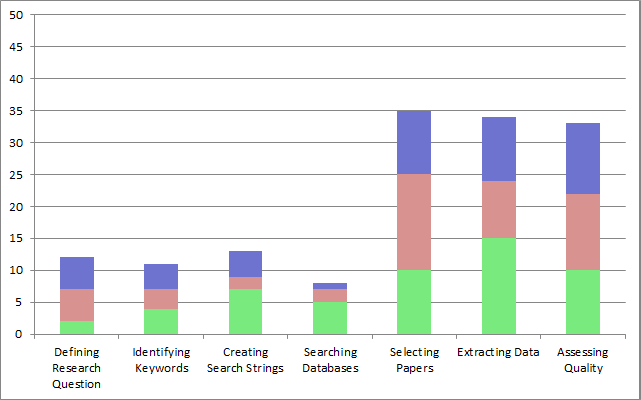
\includegraphics[width=0.48\linewidth]{difficulty.png}
        \label{fig: difficult}
    }
    \subfloat[Most Time Consuming Aspects of SLR Process.]
    {
        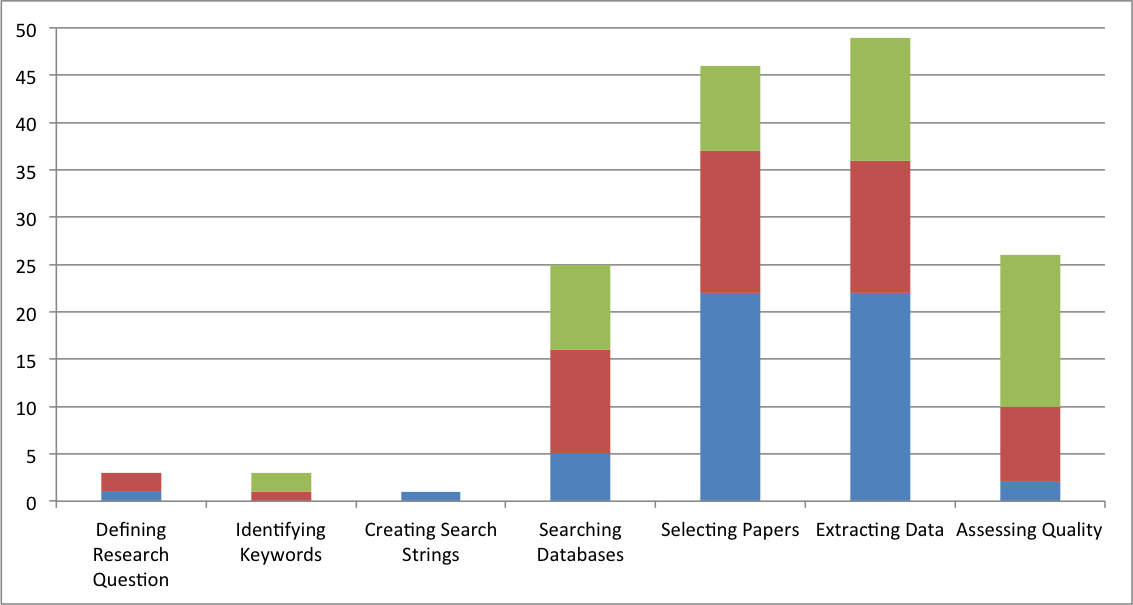
\includegraphics[width=0.48\linewidth]{time.png}
        \label{fig: time}
    }    
    \caption{Data collected from surveys to SLR authors~\cite{carver2013identifying}. Measured by number of votes, where {\setlength{\fboxsep}{1pt}\colorbox{green!40}{green}}, {\setlength{\fboxsep}{1pt}\colorbox{red!30}{red}}, and {\setlength{\fboxsep}{1pt}\colorbox{blue!50}{blue}} are number of times voted as most, second most, and third most, respectively.}
    \label{fig:barrier}
\end{figure*}
Systematic Literature Reviews
(SLRs) are one approach to this problem. SLRs are a well established and widely
applied review method in Software Engineering since Kitchenham, Dyb{\^{a}}, and
J{\o}rgensen first adopted it to support evidence-based software engineering in
2004 and 2005~\cite{kitchenham2004evidence,1377125}. 
Researchers can get a
general idea of current activity in their field of interests by reading the SLR
studies. Furthermore, a
deeper understanding of the topic may be gained by conducting an SLR.

An increasing number of SLRs has been conducted since the proposal and
revision of the SLR guidelines by Kitchenham in 2007~\cite{keele2007guidelines}. For
example, there were 26 SLRs on IEEE Xplore during the year of 2005 and that
number has increased to 137,199 for the years   2010,2015 (respectively). Various scholars  suggest that an SLR is required before any research in Software
Engineering is conducted~\cite{keele2007guidelines}.
While this is certainly a good advice,
currently an SLR is
a large, time consuming and complex
task~\cite{hassler2016identification,hassler2014outcomes,carver2013identifying,bowes2012slurp}.

Cost reduction in SLRs is therefore an important topic and will benefit researchers in software engineering community.
Previously we have analyzed the costs of SLRs~\cite{hassler2014outcomes,carver2013identifying}. As shown in Fig.~\ref{fig:barrier}, primary study selection, which is noted as ``selecting papers'' in Fig.~\ref{fig:barrier}, is among the top three most difficult
as well as time-consuming aspects in an SLR. Usually, reviewers need to evaluate
thousands of studies trying to find dozens of them that are relevant to the
research questions based on their title, abstract, or full text~\cite{bowes2012slurp}. An extreme
example of this is where reviewers sourced over
3,000 studies, and only used 7 of them in their final review~\cite{bezerra2009systematic}. The cost associated with primary study selection has become a serious problem and will continue to grow in the near future as the population of candidates for primary
studies increases dramatically. In this paper, we focus on reducing cost in primary study selection only. We prioritize primary study selection because there exists tool support for other time-consuming aspects such as searching databases~\cite{Molleri:2015:SWA:2745802.2745825,hernandes2012using}, extracting data\cite{Molleri:2015:SWA:2745802.2745825,hernandes2012using,fernandez2010slr,bowes2012slurp}, assessing quality~\cite{fernandez2010slr,bowes2012slurp,Molleri:2015:SWA:2745802.2745825}; and machine learning methods are promising in cost reduction for primary study selection~\cite{wallace2010semi,grossman2013}.

There are three main aspects in primary study selection: \textbf{(1)} retrieving initial list of primary studies, \textbf{(2)} excluding irrelevant studies, \textbf{(3)} including missing studies. We focus on excluding irrelevant studies because \textbf{a)} there already exists techniques and tools to facilitate \textbf{(1)} and \textbf{(3)} such as Snowballing~\cite{jalali2012systematic} and StArt~\cite{hernandes2012using}; \textbf{b)} the performance of excluding irrelevant studies can be evaluated using existing SLR publications.

In the SE research community, linear manual review, which requires reviewer to review every candidate study, is still the standard approach for primary study selection~\cite{kitchenham2013systematic}. On the other hand, machine learning algorithms, especially active learning, have been intensively studied to solve similar problems in other fields outside the SE research community in evidence-based medicine~\cite{paynter2016epc,wallace2010semi,wallace2010active} and in
legal electronic discovery~\cite{cormack2014evaluation,cormack2015autonomy}. This paper:
\begin{itemize}
\item
Reviews those methods. We find that in evidence-based medicine and legal electronic discovery, there are three widely recognized state-of-the-art active learning methods~\cite{cormack2014evaluation,wallace2010semi,miwa2014reducing}.
\item
Those three methods are assembled from four lower-level techniques including a) when to start training; b) query strategy; c) when/whether to stop training; d) data balancing. By analyzing techniques applied in the three methods, we generate 32 possible treatments.
\item
This paper explores all 32 treatments using data taken from the SE literature. Each treatment is evaluated by ``work saved over sampling at 95\% recall'' (WSS@95)~\cite{cohen2011performance}. 
\item
We find that one of those treatments, which we will call FASTREAD, robustly achieves the highest rank of performance across every dataset.
\end{itemize}
Interestingly, the FASTREAD treatment is not one of those used
in~\cite{cormack2014evaluation,wallace2010semi,miwa2014reducing}-- which is to say that the SE literature has nuanced differences to other kinds of literature and we should not just blindly
apply methods from other fields without certifying them on local data.
Using FASTREAD, hundreds to thousands of abstract reviewing can be avoided by sacrificing 5\% recall. That is, FASTREAD can dramatically reduce the cost of primary study selection in SE SLRs.

To assess those 32 treatments,
we need some ``gold sets'',
on which we can compare different combinations. Fortunately, in the arena of software engineering, there exist very prominent ``gold sets'' as published SLRs. This paper used three  primary study selection datasets by using the search strings and final inclusion list in such SLRs: Wahono et al. 2015~\cite{wahono2015systematic}, Hall et
al. 2012~\cite{hall2012systematic}, and Radjenovi{\'c} et al. ~\cite{radjenovic2013software}. These three SLRs are arbitrarily chosen from the set of SLR publications which define their work in enough details for us to construct datasets for simulations. Besides the three synthetic datasets, one set from Kitchenham et al. 2010~\cite{kitchenham2010systematic} has also been provided for the simulations. More details about the ``gold
sets'' will be presented later in Section~\ref{sect: datasets}. Using
these ``gold sets'', we ask and answer the following three research questions:

\begin{itemize}


\item
{\bf RQ1: Can active learning techniques reduce cost in primary study selection?} First of all, the effectiveness of active learning should be tested against traditional linear review. The rest of the research questions should not be investigated until active learning has been proved to be useful for cost reduction in primary study selection.

\item
{\bf RQ2: Should we just adopt the state-of-the-art treatments from other fields? Is it possible to build a better one by mixing and matching from those?} Active learning methods have been explored in other fields. Each of the state-of-the-art methods has its own advantage and thereby a better method might be derived by mixing and matching from those. 

\item
{\bf RQ3: How much effort can FASTREAD, our new state-of-the-art method for primary study selection, save in an SLR?} Details should be provided so that reviewers can decide whether to use FASTREAD or not.


\end{itemize}
The main contributions of this paper are:
\begin{itemize}
\item
  A demonstration of the value of  machine learning techniques for assisting primary study selection in SE SLRs.
\item
  The development of FASTREAD, a new state-of-the-art active learning method for primary study selection in SE SLRs, by refactoring three state-of-the-art methods from evidence-based medicine and electronic discovery.
  
\item
  The evaluation of our new method. The experiments shown below indicate that FASTREAD saves large amount of review efforts on primary study selection.
\item The development of a simple tool to implement FASTREAD for primary study selection.
  This tool is explained in Section~\ref{sect: tool} and is
  available for download on GitHub\footnote{https://github.com/fastread/src}. 
\end{itemize}










\section{Frequently Asked Questions}
\label{sect: Frequently Asked Questions}

When we discuss FASTREAD with our colleagues, several issues are commonly raised. This section discusses these issues.

\subsection{What about the other costs associated with SLRs?}

Our focus on the cost reductions of primary study selection is not to discount the effort associated with other parts of the SLR process. As mentioned in our introduction, we focus here on primary study selection since our data (from Fig.~\ref{fig:barrier}) indicates that this is a major component of SLR cost. 

In addition, there are tools support other components of SLRs and techniques facilitating primary study selection in different approaches. All these techniques (such as Quasi-Gold Standard based search~\cite{zhang2011empirical,zhang2011identifying}, visual text mining~\cite{Felizardo:2014:VAA:2601248.2601252,felizardo2012visual,felizardo2010approach,malheiros2007visual}, and snowballing~\cite{wohlin2014guidelines,jalali2012systematic}) are compatible and a better performance is expected when applied together. This leads to a direction of future work in which the best setting to integrate different techniques will be explored.

\subsection{What is missed?}

Our results will show, with FASTREAD, $95\%$ of the ``relevant'' studies can be retrieved by reviewing a small portion (usually hundreds of studies) of long candidate study list. Given that, it is wise to reflect
on the 5\% of papers {\em not} found by such an analysis. To this end, we took one of our case studies and reflected on:
\begin{itemize}
\item The set of papers $P_0$ that a human analyst declared to be ``relevant'' (as listed in their reference list at the end of their paper);
\item The {\em tangentially relevant} subset of those  papers $P_1 \subseteq P_0$ that a human analyst explicitly mentions, however briefly, in the body of their paper;
\item The yet smaller subset of those papers $P_2 \subseteq P_1$  that a human analyst discusses, at length, in the body of their report (and for
our purposes ``at length'' will be ``more that two lines''). We call these {\em insightful papers}. Clearly, FASTREAD should not be recommended if our method always misses the insightful papers, 
\end{itemize}
For the case studies shown below, on 30 repeats of our methods, we found that $|P_2|=0$; i.e. FASTREAD never missed an insightful paper. As for the tangentially
relevant papers, FASTREAD found all of those in 95\% of the 30 repeats. 
Based on this analysis, we infer that missing  $15\%$ of the papers is not a major impediment to using FASTREAD. Similar conclusion was derived by Shemilt et al. in 2016~\cite{shemilt2016use}.

That said, it is still true that if the SLR conductor does not want to miss any potential relevant study, he or she need to review all the candidate studies with full cost. We are actively exploring possibilities to mitigate or compensate the missing studies issue. 

% Data imbalance is explored further in Fioravanti and Nesi
% [[43]] and Zhang et al..

% Nikora and Munson [[126]] says that “without a widely agreed definition of severity
% we cannot reason about it” and Ostrand et al.
 

\subsection{What about domain knowledge?}

In our simulations, we assume that no initial seed training set is available thus a random sampling is performed to collect the minimum training set. This assumption represents the worst case while no external knowledge is available. We show in this work that the absence of that domain knowledge is not a critical failing of the approach. On the other hand, such domain knowledge usually exists in real world SLRs and will boost the performance of FASTREAD if wisely used. For example, if one relevant example and one irrelevant example are known in the very beginning, the random sampling step of FASTREAD is no longer needed and thus leads to additional cost reduction. More details about how to wisely use domain knowledge to boost FASTREAD will be explored further after this work. While we have some preliminary results in that area, we have nothing definitive to report at this time.

\subsection{What about real human reviewers?}

In our simulations, we assume that there is only one reviewer who never make mistakes. In real world SLRs, there will be multiple reviewers who make some mistakes. 

First, consider we have multiple reviewers but no mistakes. The schema of FASTREAD can be changed to one central learner with multiple review agents. Every agent reviews different studies and feedback his or her decisions to the central learner. The central learner then trains on the feedback of every agent and assigns studies to each agent for review. Such schema will keep all the property of single reviewer FASTREAD and performs similarly. In addition, there might be more intelligent way to allocate review tasks based on the different performance of review agents. Such possibility is worth exploring in future works and there already exists some studies on this topic in evidence-based medicine~\cite{wallace2011should}.

Second, consider those multiple reviewers now make mistakes. Candidate studies need to be reviewed by multiple reviewers in case any of them makes mistakes. To explore this issue, appropriate data need to be collected on how human reviewers make mistakes. Wallace et al. addressed this issue in~\cite{nguyen2015combining} by analyzing the best policy for allocating review tasks to reviewers with different experience levels as well as difference costs. We also plan to to address this issue in our future work.


\subsection{What about multiple categories of studies?}

In our simulations, we assume that the target is binary classification. However, primary study selection in real world SLRs might be a multi-label classification problem. For example, an SLR with two research questions might go through a primary study selection while each candidate is labeled as ``relevant to RQ1'', ``relevant to RQ2'', or ``irrelevant'' while the first two labels can co-exist. The simplest solution for this is to run multiple FASTREAD learners each learns on one label vs. others and each reviewer classify on one label only. In this case, the multi-label classification problem can be divided into multiple FASTREAD problems. Additional work such as ensemble learners can be explored in future works.

In summary, FASTREAD is an in-development technique that can be applied if the above trade-offs are acceptable. It can still be improved to further reduce cost of primary study selection and we will keep working on the issues until it becomes a reliable tool for different scenarios of SLRs.

























\section{Large Scale Literature Studies in SE}
\label{sect: Background}

\begin{figure}[t]
    \centering
    \begin{minipage}[t]{.51\linewidth}
    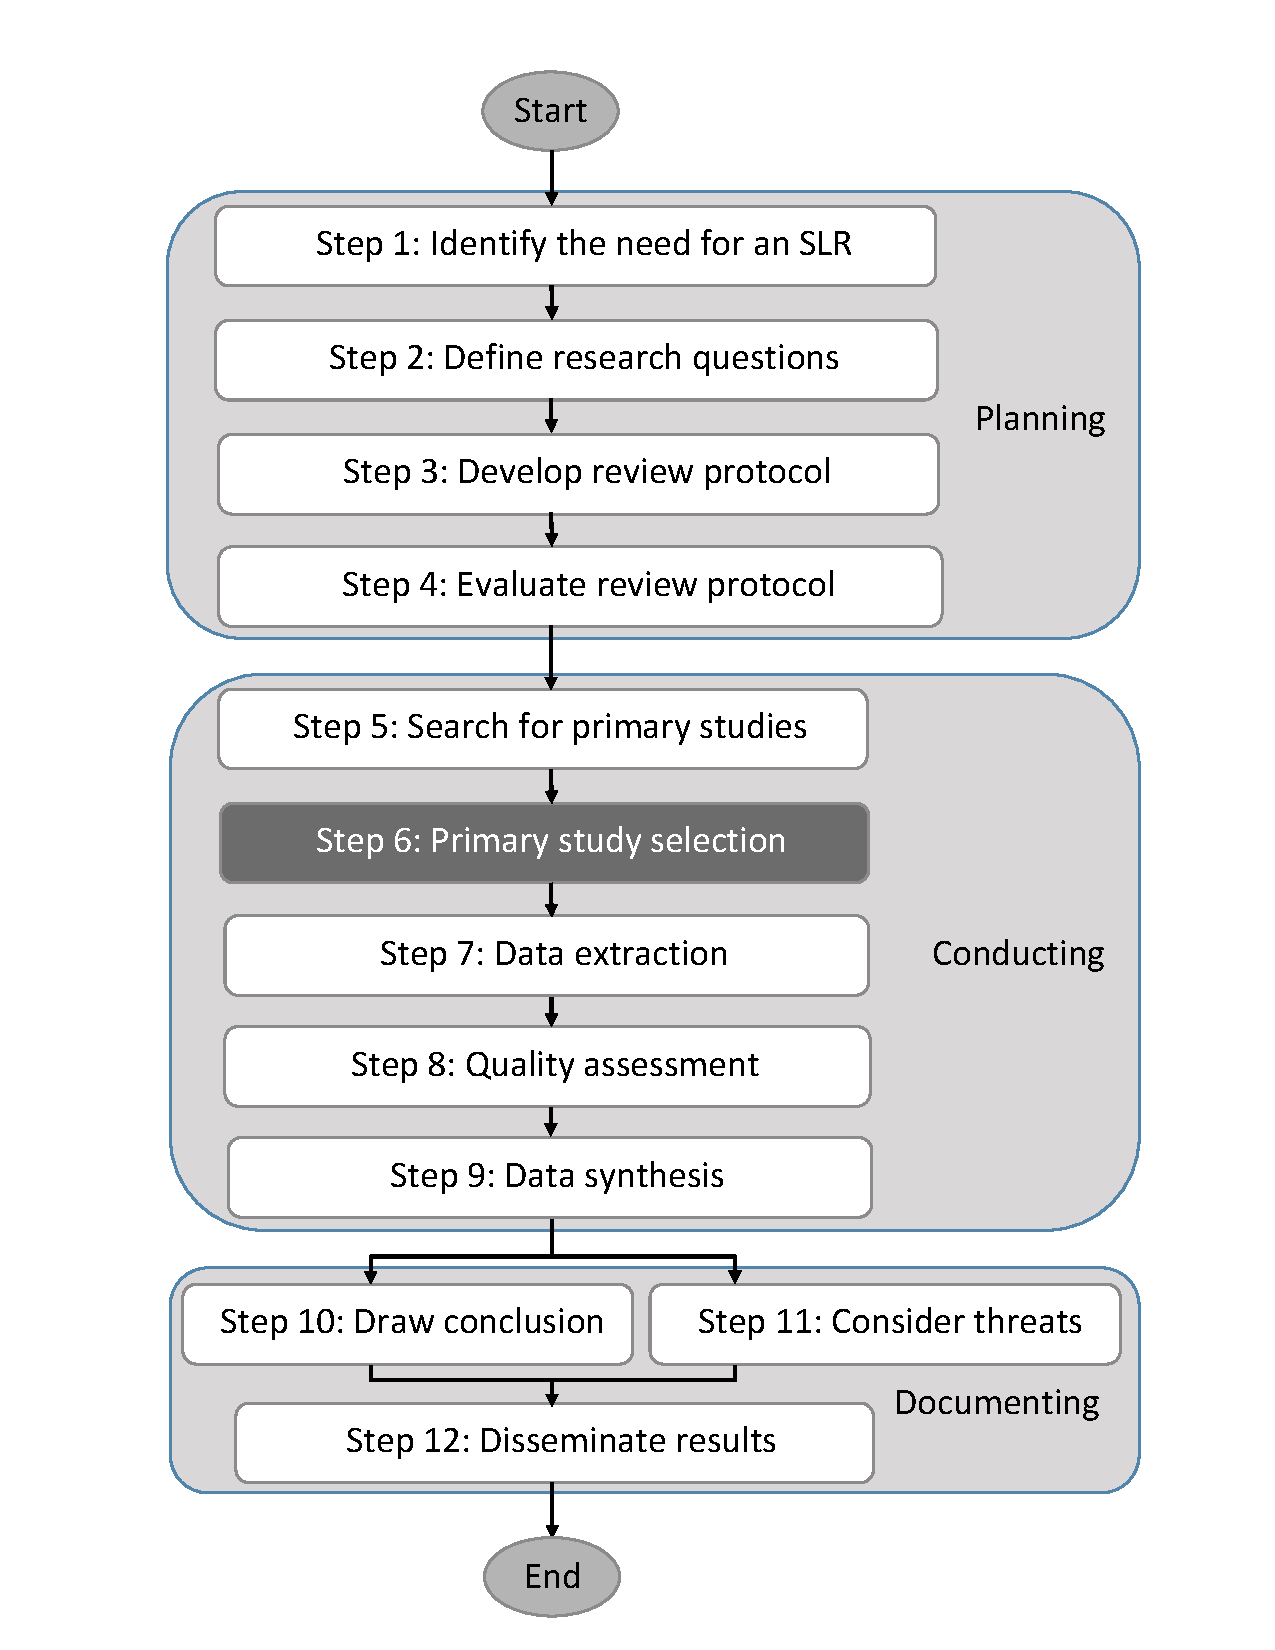
\includegraphics[width=\linewidth]{procedure.pdf}
    \caption{Systematic literature review steps suggested by~\cite{keele2007guidelines}. In this work, we focus on Step 6: primary study selection.}
    \label{fig: slr}
    \end{minipage}\quad
    \begin{minipage}[t]{.45\linewidth}
    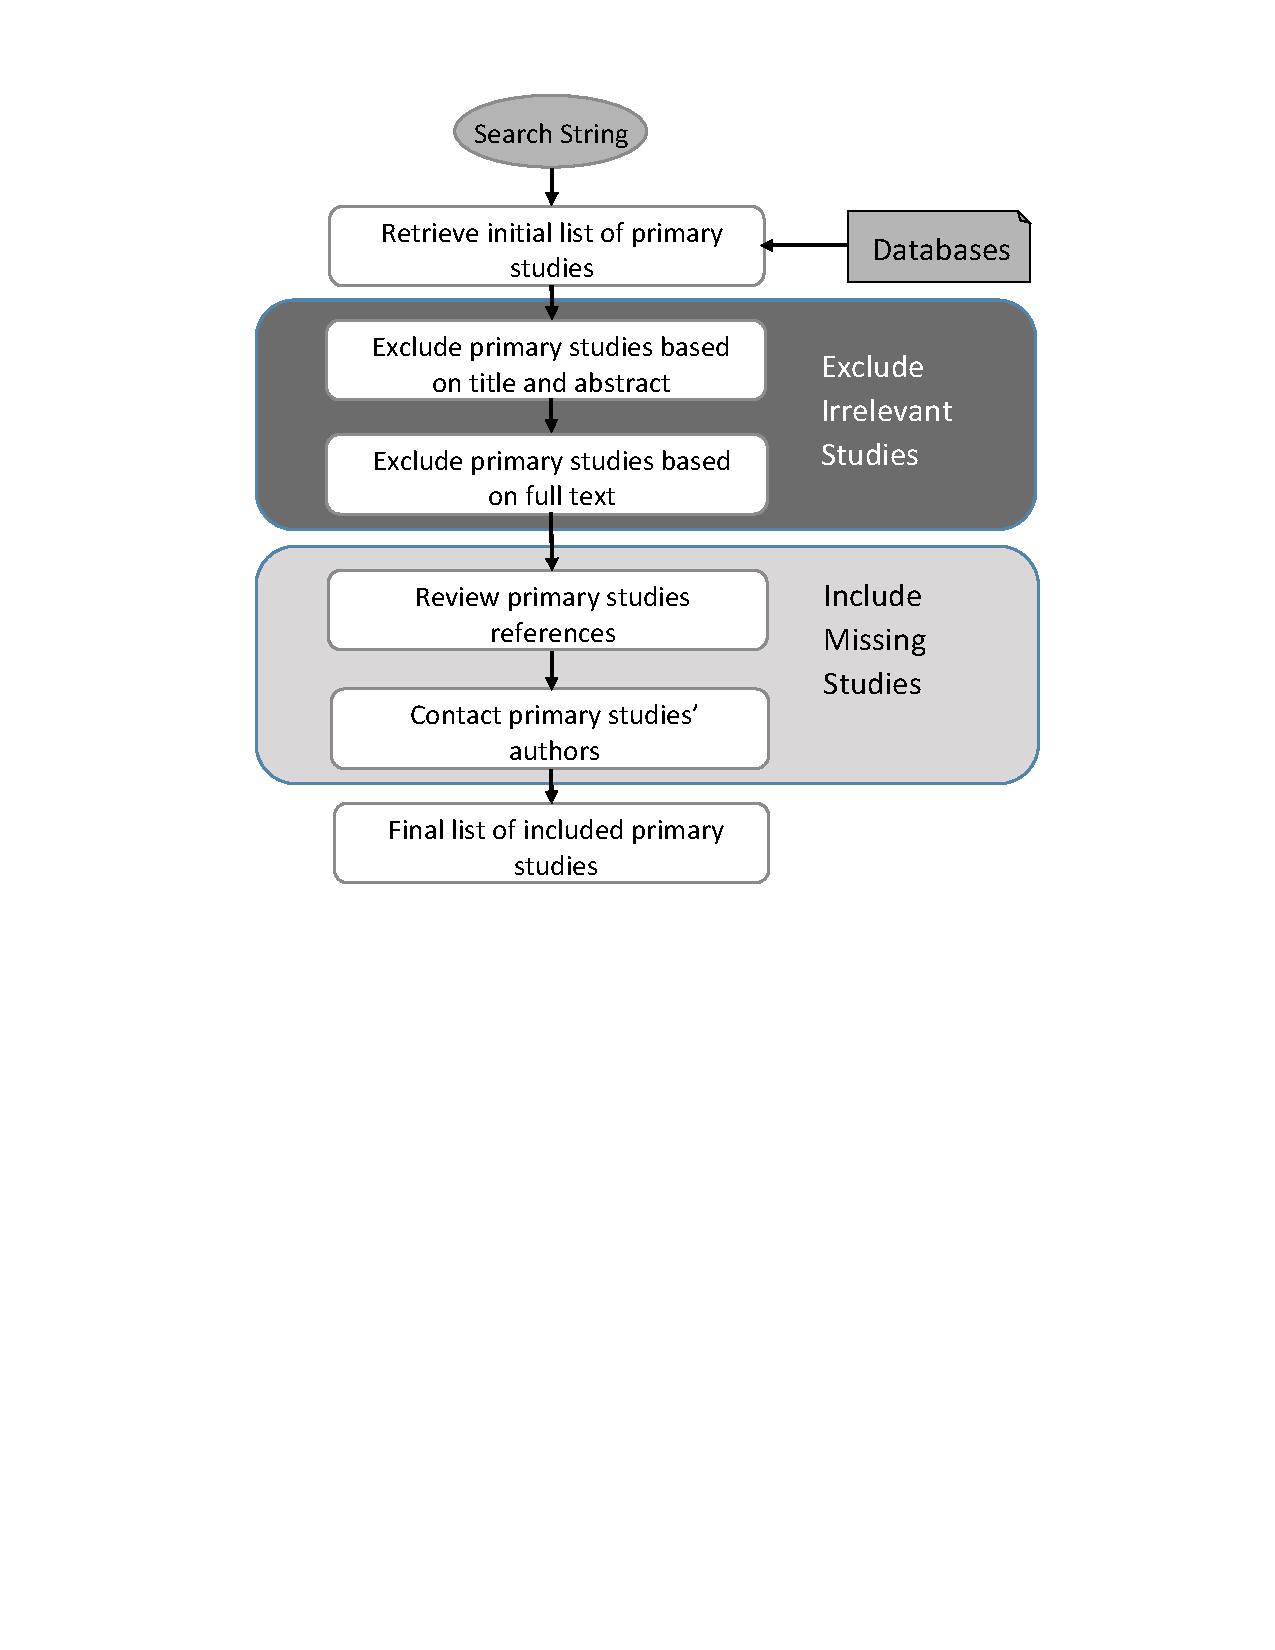
\includegraphics[width=\linewidth]{primary_study_selection.pdf}
    \caption{Primary study selection steps suggested by~\cite{keele2007guidelines}. In this work, we focus on the excluding irrelevant studies part.}
    \label{fig: prime}
    \end{minipage}
\end{figure}



% In contrast to a primary study, which investigates a specific research question,
% a systematic literature review is a form of secondary study aimed at
% identifying, evaluating and interpreting all available research relevant to a
% particular research question, topic area, or phenomenon of
% interest~\cite{keele2007guidelines}.
In the modern academic world, it is
impossible to start research without first knowing what other researchers have
done in the topic area. Conducting an SLR is one way to gain
background knowledge on a certain topic area.
If that SLR is published, then that paper becomes a useful research tool
for other researchers.  Kitchenham recommend SLRs to be standard
procedure in SE research~\cite{kitchenham2004evidence,keele2007guidelines}.

An SLR is usually conducted following the procedures in Fig.~\ref{fig: slr}. There can be variances on the real
implementations~\cite{wahono2015systematic,malhotra2015systematic,radjenovic2013software,unterkalmsteiner2012evaluation,hall2012systematic},
but all are based on the same guideline~\cite{keele2007guidelines}. Among all these steps, primary study selection is an important early step in SLRs. It starts with an initial candidate collection of studies retrieved by searching. In the first round of that process,
the reviewers' job is to read the titles and abstracts of candidate studies and classify each as ``relevant'' or ``irrelevant''. After the first round of review, the reviewers read through the full text of the previously included studies and make further decision on whether it is actually ``relevant'' or not. The whole procedure is shown in Fig.~\ref{fig: prime}. Typically, reviewers need to identify a final list of dozens of primary studies
among the initial collection of thousands of candidates. In terms of actual
cost, Malheiros has documented in~\cite{malheiros2007visual} that it requires 3
hours for one reviewer to review 100 studies.  This implies that it is a month's
work for one graduate student to review 3000 studies or three months' work to
review 9000 studies. 

In this work, we try to reduce the cost of the primary study selection by applying machine learning techniques to assist excluding irrelevant studies. In our {\em active learning} approach, each time a human reviews a paper, a learner updates its knowledge about what kind of documents are relevant. After that, the human uses that learned knowledge to guide the selection of the next paper to read.

The review cost of primary study selection can not be simply measured by the number of studies reviewed since the effort required for content review ($C_D$) is much higher than that for abstract review ($C_A$). Suppose one review process first identified $N_A$ ``relevant'' studies via reviewing $N$ abstracts, then reviewed the content of the $N_A$ studies and found $N_D$ of them are ``content relevant''. That is, to retrieve the $N_D$ ``content relevant'' studies, a total review cost of $C=N\times C_A+N_A\times C_D$ is required. To calculate this review cost, two level of relevance information is required (labels for ``abstract relevant'' and labels for ``content relevant''). However, most datasets of systematic literature review (including three datasets used in this study) have only one level of relevance information. As a result, only $N$ is used for review cost estimation since $N_A$ is not available. While this could be a fair metrics for comparing different treatments (smaller $N$ reflects less review cost in general), it is not a good estimation for how much effort saved by the text mining technique. Fortunately, the Kitchenham dataset provides two level of relevance information and we will explore the detailed review cost on this dataset in RQ3.





\subsection{Semi-Automated Tools for Literature  Reviews}

\subsubsection{Software Engineering Tools}

In recent years, various tools have been developed to facilitate SLRs in software engineering community, as summarized in~\cite{marshall2015tools,marshall2014tools,marshall2013tools}. These tools aim at providing support for protocol development~\cite{Molleri:2015:SWA:2745802.2745825,fernandez2010slr,hernandes2012using}, automated search~\cite{Molleri:2015:SWA:2745802.2745825,hernandes2012using}, primary study selection~\cite{Molleri:2015:SWA:2745802.2745825,hernandes2012using,fernandez2010slr,bowes2012slurp}, quality assessment~\cite{fernandez2010slr,bowes2012slurp,Molleri:2015:SWA:2745802.2745825}, data extraction and validation~\cite{Molleri:2015:SWA:2745802.2745825,hernandes2012using,fernandez2010slr,bowes2012slurp}, data synthesis~\cite{Molleri:2015:SWA:2745802.2745825,hernandes2012using,fernandez2010slr,bowes2012slurp},
and report write up~\cite{Molleri:2015:SWA:2745802.2745825,hernandes2012using,fernandez2010slr,bowes2012slurp}. It is extremely helpful to have a tool for managing the whole SLR process. However, the support for primary study selection using these tools is limited (e.g., to tasks such as assigning review jobs to multiple reviewers or to resolving disagreements).
Hence, we assert that the current SE SLR literature provides
no tool that can offer reductions in the effort required for primary study selection comparable to those reductions offered by active learning. Note that existing tools from Evidence-based Medicine offer active learning support and will be discussed in Section~\ref{sect: Evidence-based Medicine}.

Visual text mining (VTM) is a technique especially explored in Software Engineering community to support SLR. It is an unsupervised learning method which visualizes the relationship between candidate studies and helps the reviewer to make quick decisions. Malheiros et al.~\cite{malheiros2007visual} first applied VTM to support primary study selection in SLR. In their small-scale experiment (100 candidate studies, 31 of which are ``relevant''), VTM retrieves around 90\% of the ``relevant'' studies by spending about 30\% as much time as manual review. However, VTM requires some prior experience and knowledge of text mining and visualization techniques to use~\cite{bowes2012slurp}, and more case studies with large scale are needed to validate their results. 


Snowballing is another technique attracting much attention in SE SLR research. Given the inherent relevance relationship between a study and its citations, it is of high probability for the citations of (used in backward snowballing) and the studies cite (used in forward snowballing) a known ``relevant'' study to also be ``relevant''~\cite{kitchenham2004evidence}. Jalali and Wohlin~\cite{jalali2012systematic,wohlin2014guidelines} applied backward snowballing to search for primary studies in SE SLRs and found comparably good result as database search. Felizardo et al.~\cite{felizardo2016using} and Wohlin~\cite{wohlin2016second} applied forward snowballing to update SE SLRs and greatly reduced the number studies need to be reviewed comparing to a database search. This paper does not use snowballing since, as mentioned by Wohlin~\cite{wohlin2014guidelines}, snowballing starts with an initial set of relevant papers.
FASTREAD's task is very different: we start with zero relevant papers.



\subsubsection{Legal Electronic Discovery Tools}
\label{sect: Electronic Discovery}

Electronic Discovery (e-discovery) is a part of civil litigation where one party (the producing party), offers up materials which are pertinent to a legal case~\cite{krishna2016bigse}. This involves a review task where the producing party need to retrieve every ``relevant'' document in their possession and turn them over to the requesting party. It is extremely important to reduce the review cost in e-discovery since in a common case, the producing party will need to retrieve thousands of ``relevant'' documents among millions of candidates. Technology-assisted review (TAR) is the technique to facilitate the review process. The objective of TAR is to find as many
of the ``relevant'' documents in a collection as possible, with reasonable cost~\cite{grossman2013}. Various machine learning algorithms have been studied in TAR. So far, in every controlled studies, continuous active learning has outperformed others~\cite{cormack2014evaluation,cormack2015autonomy}, which makes it the state-of-the-art method in legal electronic discovery. It has also been selected as a baseline method in the total recall track of TREC 2015~\cite{roegiest2015trec}. Details on continuous active learning will be provided in Section~\ref{sect: Continuous Active Learning}. 

% Interestingly, the relationship between e-discovery and evidence-based medicine have been discussed in~\cite{leasesystematic} but their methods are still diverged. Relying on Grossman and Cormack~\cite{grossman2013} for support, many legal service providers have adopted TAR to facilitate the review process.

% In summary: the state-of-the-art active learning techniques are patient active learning in evidence-based medicine and continuous active learning in e-discovery.

\subsubsection{Evidence-based Medicine Tools}
\label{sect: Evidence-based Medicine}

Systematic literature reviews were first adopted from evidence-based medicine in
2004~\cite{kitchenham2004evidence}. To facilitate citation screening (primary
study selection) in systematic review, many groups of researchers have investigated different types of machine learning algorithms and evaluation mechanisms~\cite{o2015using,paynter2016epc}. 

Cohen et al. first applied text mining techniques to support citation screening and developed several performance metrics (including WSS) for assessing the performance of different techniques in 2006~\cite{cohen2006reducing}. While the great contribution of introducing machine learning and text mining into citation screening as well as the proposed performance metrics of Cohen has been widely acknowledged~\cite{o2015using}, most of Cohen's work focused on supervised learning which does not utilize unlabeled data and relies on random sampling to obtain the sufficiently large training set~\cite{cohen2006reducing,cohen2006effective,cohen2010prospective,cohen2011performance}.

Wallace et al. conducted a series of studies
with machine learning techniques, especially active
learning~\cite{wallace2010semi,wallace2010active,wallace2011should,wallace2012deploying,wallace2013active,wallace2013modernizing,nguyen2015combining}. Wallace
first set up a baseline approach called ``patient active learning'' (PAL), which will be explained later in this subsection, for machine learning assisted citation screening~\cite{wallace2010semi}. The performance of patient active learning is good enough (nearly 100\% of the ``relevant''
citations can be retrieved at half of the conventional review cost) to convince
systematic review conductors to adopt machine learning assisted citation
screening. Instead of improving this baseline method, Wallace then focused on other aspects of machine learning assisted citation screening such as introducing external expert knowledge~\cite{wallace2010active}, allocating review tasks to multiple experts~\cite{wallace2011should} or to crowdsourcing workers~\cite{nguyen2015combining}, and building a tool called abstrackr to provide overall support~\cite{wallace2012deploying}. Wallace's work on this topic is of exemplary high-impact and his core algorithm   (on simple expert screening),   is one of the most popular active learning techniques we have found in the evidence-based medical literature. That said, this technique has not been updated since 2010~\cite{wallace2010semi}. In this paper we are focused on the core active learning algorithm for cost minimization. Hence, we do not explore techniques such as Wallace's use of multiple experts (but in future work, we will explore this approach).

More recent work of Miva et al. explored alternative data balancing and query strategy in 2014~\cite{miwa2014reducing} and proposed a new treatment of Certainty plus Weighting. Instead of uncertainty sampling in PAL (and most conventional active learning approaches), Miva found that certainty sampling provides better results in clinical citation screening tasks. Similar conclusion for data balancing method as weighting relevant examples was found to be more effective than aggressive undersampling. Although not stated explicitly, Certainty plus Weighting keeps training until all ``relevant'' studies have been discovered, which differs from the stopping criteria of PAL. Aside from the core algorithm, additional views from latent Dirichlet allocation (LDA) has been found to be potentially useful.

Other work related to machine learning assisted citation screening do not
utilize active learning and active learning. Pure supervised learning requires a sufficiently large training set, which leads to a huge review cost~\cite{cohen2006reducing,adeva2014automatic}. Semi-supervised learning~\cite{liu2016comparative} does not utilize the human reviewers' feedback for updating the model, which leads to a depreciated performance in a long run. As a result, the patient active
learning proposed by Wallace et al.~\cite{wallace2010semi} and the Certainty plus Weighting approach by Miwa et al.~\cite{miwa2014reducing} are still considered to be the state-of-the-art method for citation screening in the scenario with no external knowledge and equally expensive reviewers. Details on these two approaches will be provided in Section~\ref{sect: Patient Active Learning} and \ref{sect: Certainty plus Weighting}.

There are also existing tools to support study selection in systematic reviews, e.g. Abstrakr\footnote{http://abstrackr.cebm.brown.edu}~\cite{wallace2012deploying}, EPPI-Reviewer\footnote{http://eppi.ioe.ac.uk/cms/er4/}~\cite{thomas2010eppi}, Rayaan\footnote{http://rayyan.qcri.org/}~\cite{Ouzzani2016}. Amazing features can be found in these tools such as a) Rayaan and EPPI-Reviewer: incorporated keyword search in screening; b) Rayaan and EPPI-Reviewer: deduplication; c) Rayaan and EPPI-Reviewer: define inclusion/exclusion criteria by terms; d) Abstrakr: user defined tags; e) all three: assign review tasks to multiple reviewers; f) all three: automatically extract data from PubMed. However, the active learning parts alone in these tools are depreciated. Under the condition that no additional feature (search, tags, define inclusion/exclusion terms) is used, we tried all three tools with one of our dataset-- Hall set (106 relevant in 8911 studies) and after reviewing 1000 studies, only 10 to 15 relevant ones were found, which was very close to a random sampling result without any learning. Since none of these tools are open-source, we cannot tell whether active learning is applied or how/when it is applied in each tool. This motivates us to develop an open source tool which focuses on active learning to support the primary study selection process. Details about our tool will be presented in Section~\ref{sect: tool}.



\section{Technical Notes}
\label{sect: Technical Briefing}

\begin{figure}[!t]
    \centering
    \subfloat[SVM without data balancing]
    {
        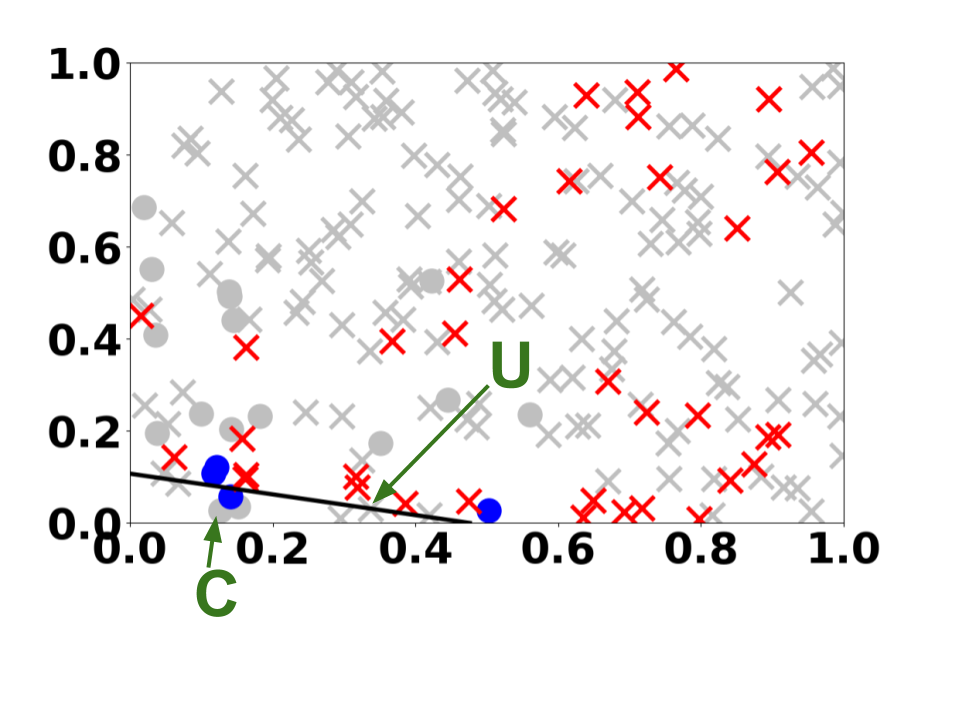
\includegraphics[width=0.3\linewidth]{simu22.png}
        \label{fig:train}
    }
    \subfloat[SVM with aggressive undersampling]
    {
        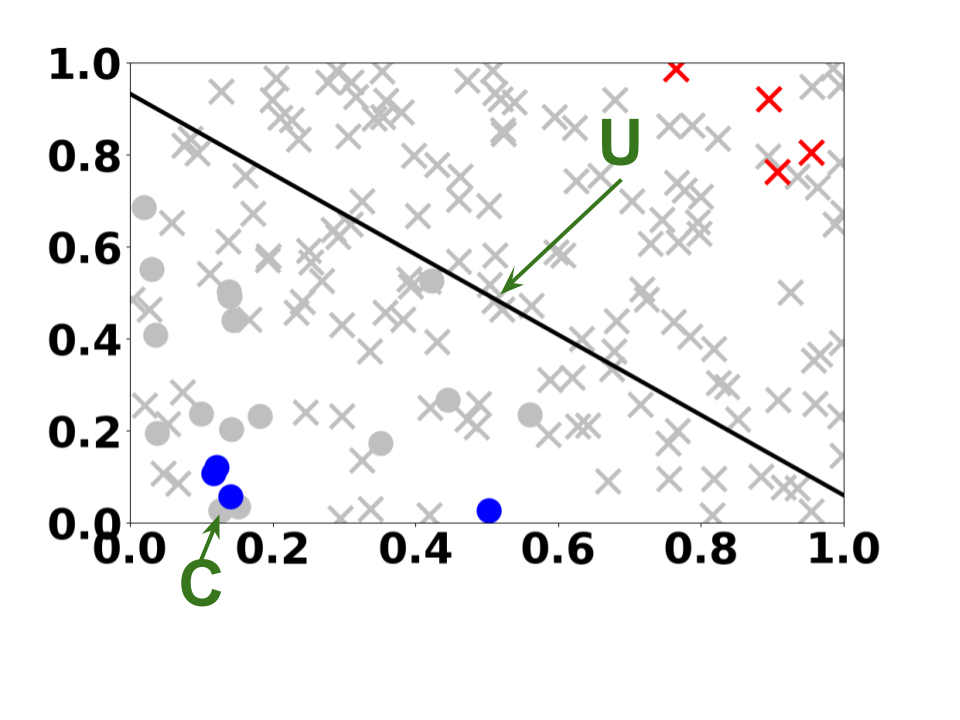
\includegraphics[width=0.3\linewidth]{simu23.png}
        \label{fig:train_a}
    }
    \subfloat[SVM with Weighting]
    {
        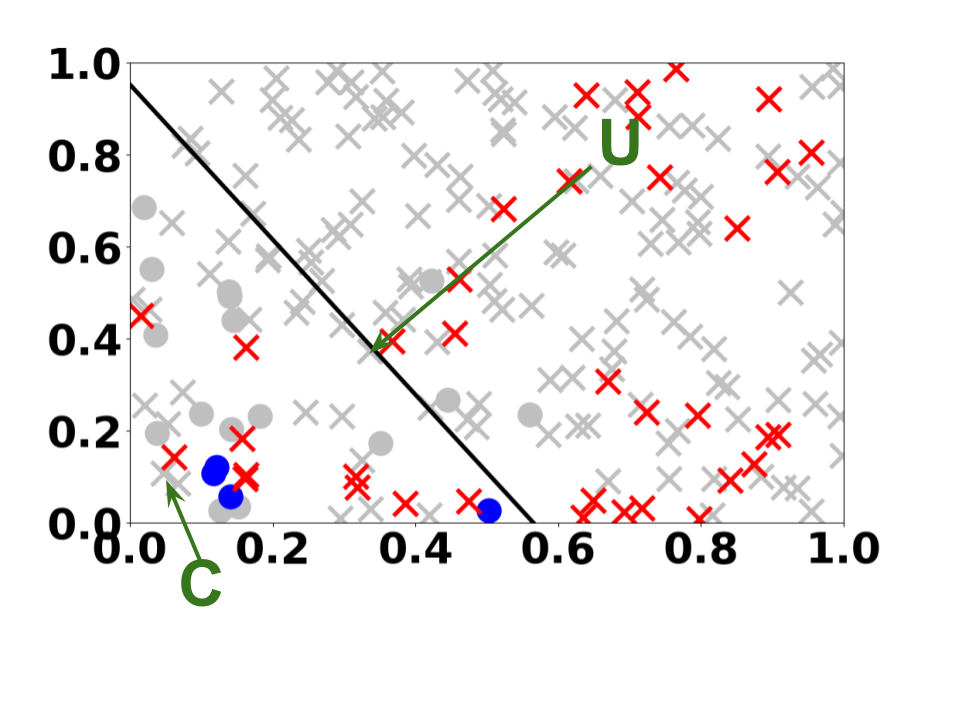
\includegraphics[width=0.3\linewidth]{simu24.png}
        \label{fig:test}
    }

    \caption{A demonstration of how SVM model is trained on imbalanced data, where ``$O$'' is the minority class, ``relevant'' studies in SLR, ``$X$'' is the majority class, ``irrelevant'' studies in SLR, markers in gray are the unlabeled studies, and black line is SVM decision plane. In (b), aggressive undersampling balances the training data by throwing away majority class examples closest to the old decision plane in (a). In (c) Weighting balances the training data by putting more weight on the minority class examples. Uncertainty sampling returns the unlabeled examples closest to the decision plane while certainty sampling returns the unlabeled examples furthest to the decision plane from the bottom-left side.}
    \label{fig:SVM}
\end{figure}

In this section, we provide details on technical terms 
used in the paper,  along with some brief introductory
notes on machine learning techniques used in this study.


\subsection{Linear Review}
\label{sect: Linear Review}

Linear review lets the reviewer to review and label every candidate study in a random order. This is still the most popular review method when there is unlimited review budget and completeness is the major objective. In this study, linear review works as a baseline method where no text mining technique is applied.

\subsection{Support Vector Machine}
\label{sect: Support Vector Machine}

Support vector machines (SVM) are a well-known and widely used classification method. The idea behind is to map input data to a high-dimension feature space and then construct a linear decision plane in that feature space~\cite{cortes1995support}. Linear SVM~\cite{joachims2006training} has been proved to be a useful model in SE text mining~\cite{krishna2016bigse} and is applied in the state-of-the-art active learning methods of both evidence-based medicine and electronic discovery~\cite{miwa2014reducing,wallace2010semi,cormack2014evaluation}. Fig.~\ref{fig:SVM} illustrates how linear SVM model is trained on a two-dimension feature space with different data balancing techniques.

\subsection{Active Learning}
\label{sect: Active learning}

Active learning is a cost-aware machine learning algorithm where labels of training data can be acquired with certain costs. The key idea behind active learning is that a machine learning algorithm can perform better with less
training if it is allowed to choose the data from which it learns~\cite{settles2012active}. There are several scenarios active learning is applied to, such as membership query synthesis, stream-based selective sampling, and pool-based sampling~\cite{settles2010active}. There are also different query strategies of active learning, such as uncertainty sampling, query-by-committee, expected model change, expected error reduction, variance reduction, and density-weighted methods~\cite{settles2010active}. Here, we will briefly introduce one scenario and two query strategies, which will be used in our later experiments and discussions.

\textbf{Pool-based sampling} is the scenario of primary study selection. This scenario starts with a fixed size pool of unlabeled data. Labels for the data can be acquired by querying an oracle selectively. The goal of pool-based sampling is to select the most informative data in the pool for query, thereby building a better model with less training.

\textbf{Uncertainty sampling} is the query strategy utilized in the state-of-the-art active learning technique of evidence-based medicine~\cite{wallace2010semi,wallace2010active}. It is also recognized as the most simple and commonly used query strategy~\cite{settles2010active}. In this query strategy, uncertainty sampling queries the instances about which the learner is least certain how to label. These instances are those (a) whose posterior probability of being positive are nearest 0.5 in probabilistic models or (b) closest to the decision boundary in models such as SVM. 

\textbf{Certainty sampling} is another query strategy which is applied in the state-of-the-art active learning technique of electronic discovery~\cite{cormack2014evaluation,cormack2015autonomy} and is also preferred over uncertainty sampling by Miwa et al. \cite{miwa2014reducing}. In contrast to uncertainty sampling, certainty sampling queries the instances about which the learner is most certain to label as positive. These instances are those (a) whose posterior probability of being positive are highest in probabilistic models, or (b) lies in the positive side of the decision boundary and furthest to the decision boundary in models such as SVM. This query strategy is usually NOT used when building the classifier of active learning since it is commonly believed that examples queried by certainty sampling contains less information than those by uncertainty sampling.

% \subsection{active Learning}
% \label{sect: active Learning}

% active learning is a combination of human decisions and machine
% suggestions~\cite{tredennick2015}. In this approach:
% \begin{itemize}
% \item
% Humans read a stream of documents, commenting on whether or
% not each one is ``relevant''.
% \item
%   Machine learners use feedback from the human opinion to
%   incrementally update their models actively.
% \item
%   The models generated via machine learning are used
%   to sort the stream of documents such that the humans focus on the
%   most informative documents.
%   \end{itemize}

% This is a
% pool-based active learning scenario since \textbf{a)} the process starts with a fixed size candidate list without any labels and \textbf{b)} training examples gradually become available to the learner as the human reviewer reviews the documents.  However, an important difference between active learning and other active learning methods is that every document labeled as ``relevant'' has been reviewed by a human. The machine never makes the final decision on whether a document is ``relevant''; a human makes such decisions and the machine only suggests a review order based on the human input. As a result, instead of building a better classification model, the objective of active learning is to retrieve most ``relevant'' documents from a pool of candidates while manually reviewing as few documents as possible. 

% Simple active learning, which is pool-based active learning with uncertainty sampling~\cite{settles2012active}, is the most basic form of learning methods
% applied to active learning. Although simple active learning achieves
% satisfactory performance, it has been outperformed by the state-of-the-art active learning techniques in both evidence-based medicine~\cite{wallace2010semi} and electronic discovery~\cite{cormack2014evaluation}. 


\subsection{Patient Active Learning}
\label{sect: Patient Active Learning}

One of the state-of-the-art active learning method in evidence-based medicine, patient active learning (PAL) can be described as following~\cite{wallace2010semi}:

\begin{itemize}

\item
{\bf Stage I: Construct an initial seed training set} by randomly sampling from the candidate study pool and asking a human reviewer to label the sampled papers as ``relevant'' or ``irrelevant''. Stop and proceed to Stage II when \textit{enough} ``relevant'' studies have been retrieved to represent the ``relevant'' class. (Note that Wallace et al.~\cite{wallace2010semi} did not provide an explicit definition of \textit{``enough''}.)

\item
{\bf Stage II: Build the classifier}, which is a linear SVM, by repeatedly training on labeled studies and uncertainty sampling. Unlabeled studies in the pool will be ranked in the descending order of uncertainty (uncertainty sampling). The human reviewer labels the studies in the ranked order and feeds them back to retrain the classifier. Stop and proceed to Stage III when the classifier is \textit{stable}. (Note that Wallace et al.~\cite{wallace2010semi} did not provide an explicit definition of \textit{``stable''}.)

\item
{\bf Stage III: Prediction.} Retrain the classifier with \textbf{aggressive undersampling} and then stop training. Unlabeled studies in the pool will be ranked in the descending order of the classifier's prediction probability of being ``relevant'' (certainty sampling as discussed in Section~\ref{sect: Active learning}). The human reviewer labels the studies in the ranked order until finished (running out of review cost budget, enough ``relevant'' studies found, or no more ``relevant'' studies are detected in multiple rounds).

\end{itemize}

{\bf Aggressive undersampling: }The data for citation screening are (at times, extremely) imbalanced, i.e., the prevalence of ``relevant'' citations is always smaller than $50\%$ (and often much smaller). Classification algorithms are typically optimized for overall accuracy, rather than accuracy, precision, recall to a particular class. This becomes a problem when only the performance on a minority class matters. Patient active learning utilizes aggressive undersampling for data balancing. By throwing away majority (``irrelevant'') class training examples which are closest to the SVM decision hyperplane, it undersamples the majority class training examples to the same size as minority (``relevant'') class. It is a recall friendly undersampling method since the new decision hyperplane is pushed away from the minority class. An exampling of aggressive undersampling is shown in Fig.~\ref{fig:SVM}.

\subsection{Certainty plus Weighting}
\label{sect: Certainty plus Weighting}

Another state-of-the-art active learning method in evidence-based medicine, Miwa et al. suggested using certainty sampling and weighting instead of uncertainty sampling and aggressive undersampling in PAL. This method can be described as following~\cite{miwa2014reducing}:

\begin{itemize}

\item
{\bf Stage I: Construct an initial seed training set} by randomly sampling from the candidate study pool and asking a human reviewer to label the sampled papers as ``relevant'' or ``irrelevant''. Stop and proceed to Stage II when \textit{enough} ``relevant'' studies have been retrieved to represent the ``relevant'' class. (Same as PAL.)

\item
{\bf Stage II: Build the classifier}, which is a linear SVM, by repeatedly training on labeled studies with \textbf{Weighting} and certainty sampling. Unlabeled studies in the pool will be ranked in the classifier's prediction probability of being ``relevant''(certainty sampling). The human reviewer labels the studies in the ranked order and feeds them back to retrain the classifier. Training continues until finished (running out of review cost budget, enough ``relevant'' studies found, or no more ``relevant'' studies are detected in multiple rounds).

\end{itemize}

{\bf Weighting: }Weighting balances the training examples by putting more weights on the minority class. The weighting factor is calculated as \emph{Size of Majority Class Training Examples / Size of Minority Class Training Examples}. An exampling of Weighting is shown in Fig.~\ref{fig:SVM}.

Miwa et al. also suggested that clustering by LDA before review has the potential to provide better performance in certain situations. However, this study focuses on refactoring and comparing the core active learning methods, same preprocessing step (without LDA) is applied to every treatment. The exploration of different feature engineering and preprocessing are planned for future works.

\subsection{Continuous Active Learning}
\label{sect: Continuous Active Learning}

The state-of-the-art active learning method in e-discovery, continuous active learning (CAL) can be described as following~\cite{cormack2014evaluation,cormack2015autonomy,tredennick2015}:

\begin{itemize}

\item
{\bf Stage I: Construct an initial seed training set} by random sampling from the candidate study pool and ask a human reviewer for labels. Stop and proceed to Stage II as soon as \textbf{ONE} ``relevant'' study is retrieved.

\item
{\bf Stage II: Predict and retrain} by repeatedly training on labeled studies and certainty sampling. Unlabeled studies in the pool will be ranked in the descending order of the classifier's prediction probability of being ``relevant'' (certainty sampling). A human reviewer labels the studies in the ranked order and feeds them back to retrain the classifier until finished.

\end{itemize}

In contrast to PAL, CAL is the opposite of ``patient''. It starts to train the model as soon as \textit{ONE} ``relevant'' study shows up and skips the uncertainty sampling stage, which is believed to be essential for active learners~\cite{settles2012active}. Since the objective is to retrieve ``relevant'' studies with candidates reviewed as few as possible, it is reasonable not to waste any single effort on building up the classifier~\cite{cormack2014evaluation,tredennick2015}. Also, the experiment results in~\cite{cormack2014evaluation} has demonstrated the value of this ``greedy'' strategy.

Among all the three state-of-the-art treatments, CAL and PAL are different in every aspect while Certainty plus Weighting is in the middle of these two and supports a different data balancing method.


\section{Methods}
\label{sect: Method}

This section describes our datasets and their preparation then describes and refactors state-of-the-art methods for active learning.
This refactoring process will create FASTREAD, our preferred active learning
method. 

\subsection{Datasets}
\label{sect: datasets}

Although a large number of SLRs are published every year, there is no dataset clearly documenting the details in primary study selection. As a result, three datasets are created based on the information in existing SLRs and being used in this study to simulate the process of excluding irrelevant studies. The three datasets are named after the authors of their original publication source-- Wahono dataset from Wahono et al. 2015~\cite{wahono2015systematic}, Hall dataset from Hall et al. 2012~\cite{hall2012systematic}, and Radjenovi{\'c} dataset from Radjenovi{\'c} et al. 2013~\cite{radjenovic2013software}. 

For each of the datasets, the search string \textbf{S} and the final inclusion list \textbf{I} from the original publication are used for the data collection. We retrieve the initial candidate collection \textbf{C} from IEEE Xplore with the search string (slightly modified to meet the requirement of IEEE Xplore). Then make a final list of inclusion \textbf{R} as \textbf{R} = \textbf{I} $\cap$ \textbf{C}. Here, for simplicity reason we only extract candidate studies from IEEE Xplore. We will explore possibilities for efficiently utilizing multiple data sources in the future work but in this paper, without loss of generality, we only extract initial candidate list from single data source. In this way, we created three datasets that reasonably resemble real SLR selection results assuming that any study outside the final inclusion list \textbf{I} is irrelevant to the original SLRs. A summary of the created datasets is presented in Table~\ref{tab: number}.

Apart from the three created datasets, one dataset (Kitchenham) is provided directly by the author of Kitchenham et al. 2010~\cite{kitchenham2010systematic} and includes two levels of relevance information. In general, only the ``content relevant'' labels are used in experiments for a fair comparison with other datasets. Additionally, the ``abstract relevant'' labels are used for detailed review cost analysis in RQ3. Summary of Kitchenham dataset is also presented in Table~\ref{tab: number}.

All the above datasets are available on-line at {\em https://doi.org/10.5281/zenodo.837298}.

\begin{table}
\caption{Descriptive statistics for experimental datasets}
\label{tab: number}
\begin{center}
\begin{tabular}{ |l|c|c|c|c| }
  \hline
   Datasets & \multicolumn{2}{|c|}{Generated} & \multicolumn{2}{|c|}{Original} \\
  \cline{2-5}
  & \#Candidate $|$\textbf{C}$|$ & \#Relevant $|$\textbf{R}$|$& \#Candidate & \#Relevant $|$\textbf{I}$|$\\
  \hline
  Wahono & 7002 & 62 & 2117 & 72\\
  \hline
  Hall & 8911 & 106 & 2073 & 136 \\
  \hline
  Radjenovi{\'c} & 6000 & 48 & 13126 & 106\\
  \hline
  Kitchenham & 1704 & 44 (132) & 1704 & 44 (132) \\
  \hline
\end{tabular}
\end{center}
{\footnotesize Our datasets are generated using information in the original SLR literature. Our candidate studies are retrieved by applying similar if not the same the search string from original SLR literature and search in IEEE Xplore. The set of our relevant studies is the intersection of the set of our candidate studies and the set of final included studies in the original SLR literature. Kitchenham dataset is different as it is provided directly by Kitchenham and it has two level of relevance labels-- 132 relevant studies by title and abstract review and within which, 44 relevant studies by content review.}
\end{table}




\begin{figure}[t]
    \centering
    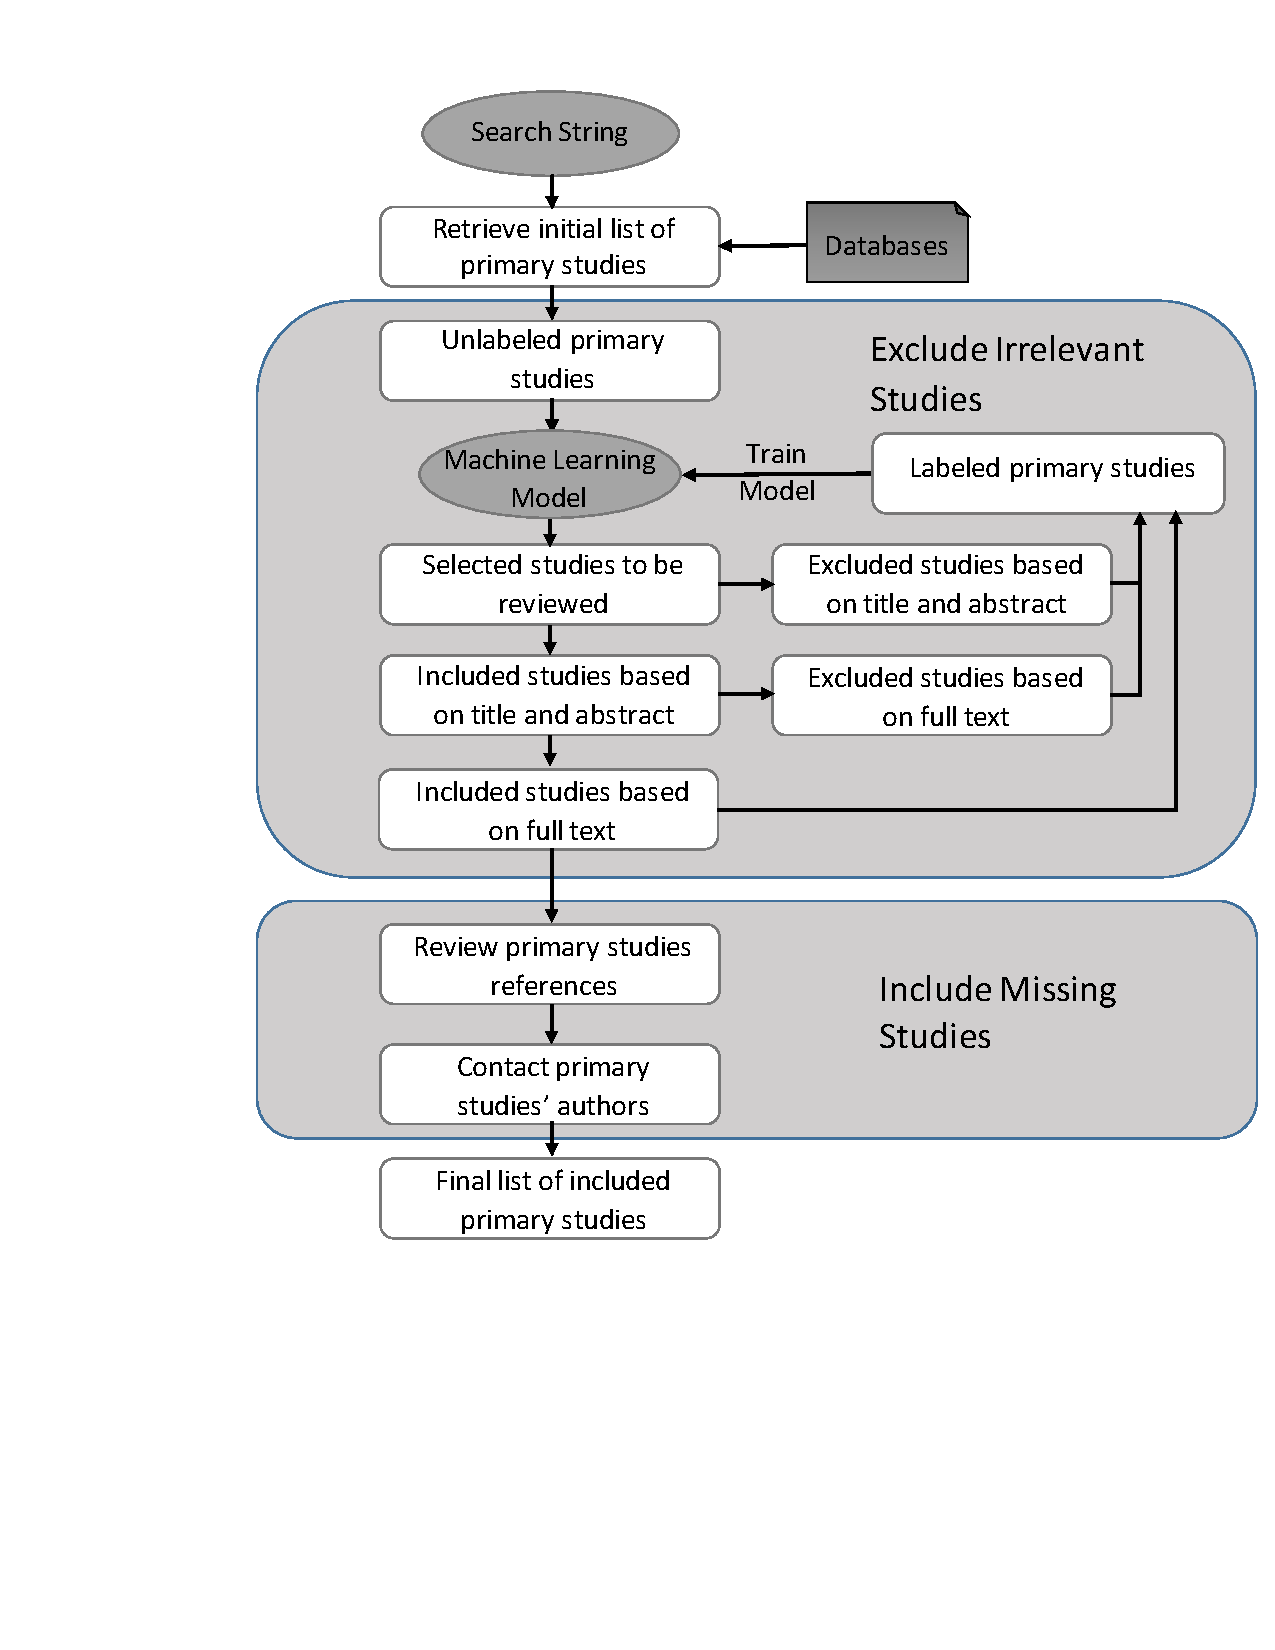
\includegraphics[width=0.6\linewidth]{Learning_based_primary_study_selection.pdf}
    \caption{Human-in-the-loop Primary study selection.}
    \label{fig: learning}
\end{figure}

\subsection{Human-in-the-loop Primary Study Selection}
\label{subsect: Learning based Primary Study Selection}


In contrast to the classical primary study procedures in Fig.~\ref{fig: prime}, with active learning as part of the process, the general form of human-in-the-loop primary study selection is presented in
Fig.~\ref{fig: learning}. Reviewers first review the title and abstract of the
suggested study, determine whether it is ``abstract relevant'' or ``abstract irrelevant''. If the study is relevant by title and abstract, the reviewer will then read the full text of the study and make the final decision-- ``content relevant'' or ``content irrelevant''. In the meantime, all the reviewed
studies will go into the training set. Note that only the title and abstract of the training set studies will be used to train the active learning model, thus making data extraction for training examples easy. Note that in this process, two-level relevance labels are generated and should be available to the active learning model. However, the fact is, for most of our datasets, ``abstract relevant'' labels are missing since they are not reported in the original SLR literature. As a result, only ``content relevant'' labels are being used for training in our experiments. In the rest of the paper, when we say ``relevant'', it means ``content relevant'' while ``irrelevant'' studies include every study that is not ``content relevant'' (``abstract relevant'' but ``content irrelevant'' or ``abstract irrelevant'').

The objective of Human-in-the-loop primary study selection (or machine learning
assisted citation screening or TAR) is different from that of common active
learning scenarios. Instead of trying to build a classifier as good as possible,
human-in-the-loop primary study selection seeks methods to retrieve most
``relevant'' studies with candidate studies reviewed as few as possible. This
difference in the objective leads to a different performance metrics (further explained in Section~\ref{subsect: Performance Metrics}) and thus
makes conventional active learning methods being outperformed by specially
designed methods like PAL~\cite{wallace2010semi}, Certainty plus Weighting~\cite{miwa2014reducing} in evidence-based
medicine and CAL~\cite{cormack2014evaluation,cormack2015autonomy} in
e-discovery.



\subsection{Algorithm Code}
\label{sect: Algorithm Code}

Differences of the three state-of-the-art active learning techniques for systematic reviews are from four aspects: 1) when to start training; 2) query strategy; 3) whether to stop training; 4) data balancing.

\begin{itemize}

\item
{\bf When to start training}: 

\textbf{P} stands for ``patient''. As suggested by Wallace et al.~\cite{wallace2010semi}, ``hasty generation'', which means start training with too few relevant examples, may leads to deteriorate performance. The algorithm keeps random sampling until a sufficient number of ``relevant'' studies retrieved. In our experiments, the sufficient number of ``relevant'' studies retrieved is set to $5$, which means when at least $5$ ``relevant'' studies have been retrieved by random sampling, the algorithm goes into next stage. PAL~\cite{wallace2010semi} and Certainty plus Weighting~\cite{miwa2014reducing} use \textbf{$P$} for when to start training.

\textbf{H} is the opposite. The algorithm stops random sampling as long as {\em ONE} ``relevant'' studies are retrieved, as suggested in CAL~\cite{cormack2014evaluation,cormack2015autonomy}.

\item
{\bf Query strategy}: 

\textbf{U} stands for ``uncertainty sampling''. The algorithm utilizes
uncertainty sampling to build the classifier, where unlabeled examples closest to the SVM decision plane are sampled for query. PAL~\cite{wallace2010semi} uses \textbf{U} for Query strategy.

\textbf{C} stands for ``certainty sampling''. The algorithm utilizes certainty sampling to build the classifier, where unlabeled examples furthest to the SVM decision plane and lie in the ``relevant'' side are sampled for query. Certainty plus Weighting~\cite{miwa2014reducing} and CAL~\cite{cormack2014evaluation,cormack2015autonomy} use \textbf{C} for query strategy.

\item
{\bf Whether to stop training}: 

\textbf{S} stands for ``stop training''. The algorithm stops training
once the classifier is stable. In our experiments, the classifier is treated as stable once more than $30$ ``relevant'' studies have been retrieved as training examples. PAL~\cite{wallace2010semi} uses \textbf{$S$} for whether to stop training.

\textbf{T} stands for ``continue training''. The algorithm never stops
training as suggested in CAL~\cite{cormack2014evaluation,cormack2015autonomy} and Certainty plus Weighting~\cite{miwa2014reducing}. If query strategy is \textbf{U}, algorithm switches to certainty sampling after classifier is stable but training never stops.

\item
{\bf Data balancing}: 

\textbf{N} stands for ``no data balancing''. The algorithm does not balance the training data as suggested by CAL~\cite{cormack2014evaluation,cormack2015autonomy}.

\textbf{A} stands for ``aggressive undersampling''. The algorithm utilizes aggressive undersampling when classifier is stable, as suggested by PAL~\cite{wallace2010semi}.

\textbf{W} stands for ``Weighting''. The algorithm utilizes Weighting for data balancing (before and after the classifier is stable), as suggested by Certainty plus Weighting~\cite{miwa2014reducing}.

\textbf{M} stands for ``mixing of Weighting and aggressive undersampling''. Weighting is applied before the classifier is stable while aggressive undersampling is applied after the classifier is stable. This treatment comes from the observation that ``Weighting'' performs good in early stages while ``aggressive undersampling'' performs good in late stages.

\end{itemize}
As a result, we ended up with 32 treatments including the state-of-the-art treatments as
\begin{itemize}
\item
\textbf{PUSA}: patient active learning~\cite{wallace2010semi,wallace2010active};
\item
\textbf{PCTW}: Certainty plus Weighting~\cite{miwa2014reducing};
\item
\textbf{HCTN}: continuous active learning~\cite{cormack2014evaluation,cormack2015autonomy}. 
\end{itemize}
All the 32 algorithms are tested and compared in Section~\ref{sect: Experiments}.

\section{Experiments}
\label{sect: Experiments}

This section describes the experimental procedures that we used to evaluate the treatments described in Section~\ref{sect: Algorithm Code} on the datasets described in Section~\ref{sect: datasets}. 

There is no human activity involved in these experiments, when asked for a label, the true label in the dataset is queried instead of a human reviewer. As a result, each experiment can be repeated with different random seed to capture variances and also makes reproducing the experiments possible. Each experiment is a simulation of one specific treatment on one dataset:

\begin{enumerate}
\item
Starts with an unlabeled collection of candidate studies, e.g. 8911 in Hall as shown in Table~\ref{tab: number}.

\item
\label{select}
Train a model on current labeled examples if enough labeled examples are available.

\item
Select $N=10$ studies based on the prediction of machine learning model on unlabeled examples for review. If no model is trained yet, random sample $N=10$ unlabeled studies.

\item
Query the true labels of the selected studies, i.e. 106 ``relevant'' and 8805 ``irrelevant'' in Hall as shown in Table~\ref{tab: number}, label them as their true labels.

\item
Go back to \ref{select} until finished.

\end{enumerate}


\subsection{Controlled Variables}
\label{subsect: Controlled Variables}

For the sake of a fair comparison, different treatments in Section~\ref{sect: Algorithm Code} share an identical set of controlled variables including preprocessing, featurization and classifier. 

\subsubsection{Preprocessing and Featurization}

Each candidate study in the initial list is first tokenized by stop words removal after concatenating its title and abstract. After tokenization, the bag of words are featurized into a term frequency vector. Then, reduce the dimensionality of the term frequency vector with to keep only $M=4000$ of the terms with highest tf-idf\footnote{For term $t$ in document $d$, $Tfidf(t, d)=w^t_d\times (\log \frac{|D|}{\sum_{d\in D} sgn(w^t_d)}+1)$ where $w^t_i$ is the term frequency of term $t$ in document $d$. For term $t$, $Tfidf(t) = \sum_{d\in D} Tfidf(t,d) = \sum_{d\in D} w^t_d \times (\log \frac{|D|}{\sum_{d\in D} sgn(w^t_d)}+1)$ and is used for feature selection.} score and normalize the hashed matrix by its L2 norm each row at last. TfidfVectorizer in scikit-learn is utilized for the above preprocessing and featurization steps. Alternatives such as stemming, LDA~\cite{blei2003latent}, paragraph vectors~\cite{le2014distributed} require exploration and are scheduled in our future works. 


\subsubsection{Classifier}

For this work we use a linear SVM as the classifier.
SVMs learn a hyperplane that separate relevant from irrelevant examples
in the training data. Linear SVMs do not make complicated assumptions about the data space and so are known to scale to very large, high-dimensional problems~\cite{joachims2006training}. Such linear SVMs are widely used in the state-of-the-art solutions~\cite{miwa2014reducing,cormack2015autonomy,wallace2010semi}. SVM's hyperplane is a natural tool for deciding what examples to show next to the human user. As discussed in Section~\ref{sect: Technical Briefing}, uncertainty sampling prefers the examples {\em closest} to the hyperplane boundary since these are the ones whose classification will
change, given small changes to the test data. On the other hand, certainty sampling prefers the examples with {\em highest} SVM predictions of being positive. SVC (set to be linear kernel) with default parameters in scikit-learn is utilized as the classifier.


\subsection{Performance Metrics}
\label{subsect: Performance Metrics}

Common active learning aims for building a better model with less training. Therefore, its performance metrics is usually some \textbf{accuracy, precision, recall} on the model prediction vs \textbf{training size} curve. The \textbf{accuracy, precision, recall} are measured on some validation set.

On the other hand, since the goal of human-in-the-loop primary study selection described in Section~\ref{subsect: Learning based Primary Study Selection} is different from that of common active learning, the performance metrics is also different. In human-in-the-loop primary study selection, the performance of each algorithm is evaluated by its \textbf{recall} vs. \textbf{studies reviewed} curve. The \textbf{recall} here is not a measurement on the trained model, but the number of ``relevant'' studies retrieved over the total number of ``relevant'' studies. An algorithm is better than the other if it can retrieve more ``relevant'' studies with fewer studies reviewed. This performance metrics is suggested by~\cite{cormack2015autonomy,cormack2014evaluation,tredennick2015} and best fits the objective of human-in-the-loop primary study selection. To enable a statistical analysis of the performances, the \textbf{recall} vs. \textbf{studies reviewed} curve is cut by a $0.95$ \textbf{recall} line and \textbf{studies reviewed} when reaching $0.95$ \textbf{recall} is used to assess performances. The reason behind $0.95$ \textbf{recall} is that a) $1.00$ \textbf{recall} can never be guaranteed by any text mining method unless all the candidate studies are reviewed; b) $0.95$ \textbf{recall} is usually considered acceptable in evidence-based medicine~\cite{cohen2011performance,cohen2006reducing,o2015using} despite the fact that there might still be ``relevant'' studies missing~\cite{shemilt2016use}. As a result, two numbers are recorded during experiments:
\begin{itemize}
\item
X95 = $\min \{x | r(x)\geq0.95 R\}$
\item
WSS@95 = $0.95-\text{X95}/T$
\end{itemize}
where in a total number of $T$ candidate studies, $R$ of them are ``relevant'' according to true labels, and $r(x)$ is the number of ``relevant'' studies found when $x$ studies have been reviewed.

Each treatment on each dataset is tested for 30 repeats\footnote{It is suggested that usually a sampling size of $30$ is adequate~\cite{isotalo2001basics}.} with random seeds ranging from 0 to 29. The 30 records collected for each treatment on each dataset are then used for comparison through Scott-Knott analysis as recommended by Mittas \& Angelis in their 2013 IEEE TSE paper~\cite{mittas2013ranking}. Scott-Knott clusters methods with little difference in performance together and rank each cluster with the median performances~\cite{scott1974cluster}. Since the 30 records for each treatment on each dataset do not follow a normal distribution, we utilize nonparametric hypothesis tests. Scott-Knott decides two methods are not of little difference if both bootstrapping~\cite{efron1982jackknife} and an effect size test~\cite{cliff1993dominance} agreed that the difference is statistically significant ($99\%$
confidence) and not a “negligible” effect (Cliff's Delta $\ge$ 0.147).





\subsection{Results}
\label{subsect: Results}


\begin{table*}
\caption{Scott-Knott analysis for number of studies reviewed/ work saved over sampling to reach $95\%$ recall}
\label{tab: scottknott}


\begin{center}
\parbox{.49\linewidth}{
\centering
{\scriptsize \begin{tabular}{l@{~~~}l@{~~~}r@{~~~}r@{~~~}r@{~~~}r}
\arrayrulecolor{lightgray}
\multicolumn{2}{l}{\textbf{Wahono}}  & \multicolumn{2}{c}{\textbf{X95}} & \multicolumn{2}{c}{\textbf{WSS@95}}\\\hline
\textbf{Rank} & \textbf{Treatment} & \textbf{Median} & \textbf{IQR} & \textbf{Median} & \textbf{IQR} \\\hline
\rowcolor{green!40}
  1 &         HUTM &    670  &  230 & 0.85 & 0.04 \\
  1 &         HCTM &    740  &  220 & 0.84 & 0.03 \\
\hline  2 &         HUTA &    780  &  140 & 0.84 & 0.02 \\
  2 &         HCTW &    790  &  90 & 0.84 & 0.02 \\
  2 &         HUTW &    800  &  110 & 0.84 & 0.02 \\
  2 &         HCTA &    800  &  140 & 0.83 & 0.02 \\
\hline  3 &         PCTM &    1150  &  450 & 0.78 & 0.07  \\
  3 &         PUTM &    1180  &  420 & 0.78 & 0.07 \\
  3 &         PCTA &    1190  &  340 & 0.78 & 0.05 \\
  3 &         PUTA &    1190  &  340 & 0.78 & 0.05 \\
\rowcolor{red!30}
  3 &         PCTW &    1210  &  350 &  0.78 & 0.06 \\
  3 &         PUTW &    1220  &  370 &  0.77 & 0.06 \\
\hline  4 &         HUSM &    1410  &  400 & 0.75 & 0.06 \\
\hline  5 &         HUSA &    1610  &  370 & 0.72 & 0.07 \\
\hline  6 &         PUSM &    1810  &  370 & 0.69 & 0.06 \\
\rowcolor{red!30}
  6 &         PUSA &    1910  &  700 & 0.67 & 0.10 \\
\hline  7 &         HUSW &    2220  &  400 & 0.63 & 0.06 \\
  7 &         PUSW &    2240  &  360 & 0.63 & 0.06 \\
\hline  8 &         HUTN &    2700  &  40 & 0.56 & 0.01 \\
\rowcolor{red!30}
  8 &         HCTN &    2720  &  40 & 0.56 & 0.01 \\
  8 &         PCSW &    2860  &  1320 & 0.54 & 0.20 \\
  8 &         PCSM &    2860  &  1320 & 0.54 & 0.20 \\
  8 &         PCTN &    2850  &  1130 & 0.54 & 0.17 \\
  8 &         PUTN &    2850  &  1130 & 0.54 & 0.17 \\
\hline  9 &         PCSN &    3020  &  1810 & 0.51 & 0.26 \\
  9 &         PCSA &    3020  &  1810 & 0.51 & 0.26 \\
\hline 10 &         HUSN &    4320  &  110 &  0.33 & 0.03 \\
 10 &         PUSN &    4370  &  1290 & 0.32 & 0.19 \\
 \rowcolor{blue!50}
\hline 11 &       linear &    6650  &  0 & 0 & 0 \\
 11 &         HCSA &    6490  &  2760 & -0.01 & 0.39 \\
 11 &         HCSN &    6490  &  2760 & -0.01 & 0.39 \\
 11 &         HCSM &    6490  &  3110 & -0.01 & 0.44 \\
 11 &         HCSW &    6490  &  3110 & -0.01 & 0.44 \\
\hline \end{tabular}}
}
\parbox{.49\linewidth}{
\centering
{\scriptsize \begin{tabular}{l@{~~~}l@{~~~}r@{~~~}r@{~~~}r@{~~~}r}
\arrayrulecolor{lightgray}
\multicolumn{2}{l}{\textbf{Hall}}  & \multicolumn{2}{c}{\textbf{X95}} & \multicolumn{2}{c}{\textbf{WSS@95}}\\\hline
\textbf{Rank} & \textbf{Treatment} & \textbf{Median} & \textbf{IQR} & \textbf{Median} & \textbf{IQR} \\\hline
  1 &         HUTW &    350  &  80 & 0.91 & 0.01 \\
  1 &         HUTA &    360  &  140 & 0.91 & 0.02 \\
  \rowcolor{green!40}
  1 &         HUTM &    360  &  140 & 0.91 & 0.02 \\
  1 &         HCTW &    370  &  50 & 0.91 & 0.01 \\
\hline  2 &         HCTM &    400  &  90 & 0.90 & 0.01 \\
  2 &         HCTA &    410  &  140 & 0.90 & 0.02 \\
  2 &         HUTN &    430  &  100 & 0.90 & 0.01 \\
  \rowcolor{red!30}
  2 &         HCTN &    460  &  70 & 0.90 & 0.01 \\
\hline  3 &         HUSM &    630  &  160 & 0.88 & 0.03 \\
\rowcolor{red!30}
  3 &         PCTW &    640  &  190 & 0.88 & 0.02 \\
  3 &         PUTW &    640  &  220 & 0.88 & 0.03 \\
\hline  4 &         PCTN &    680  &  210 & 0.87 & 0.03 \\
  4 &         PUTN &    680  &  200 & 0.87 & 0.03 \\
  4 &         PUTM &    690  &  230 & 0.87 & 0.03 \\
  4 &         PCTA &    730  &  260 & 0.87 & 0.03 \\
  4 &         PCTM &    720  &  230 & 0.87 & 0.03 \\
  4 &         PUTA &    730  &  230 & 0.87 & 0.03 \\
\hline  5 &         HUSW &    790  &  320 & 0.86 & 0.04 \\
  5 &         HUSA &    790  &  200 & 0.86 & 0.03 \\
  5 &         PUSW &    840  &  280 & 0.86 & 0.03 \\
  5 &         PUSM &    860  &  320 & 0.85 & 0.04 \\
  \rowcolor{red!30}
  5 &         PUSA &    970  &  310 & 0.84 & 0.04 \\
\hline  6 &         PCSW &    1560  &  580 & 0.77 & 0.07 \\
  6 &         PCSM &    1560  &  580 & 0.77 & 0.07 \\
\hline  7 &         PUSN &    1680  &  1390 & 0.76 & 0.18 \\
  7 &         PCSN &    1990  &  690 & 0.72 & 0.09 \\
  7 &         PCSA &    1990  &  690 & 0.72 & 0.09 \\
\hline  8 &         HUSN &    2270  &  1230 & 0.69 & 0.16 \\
\hline  9 &         HCSA &    7500  &  5170 & 0.03 & 0.58 \\
  9 &         HCSN &    7500  &  5170 & 0.03 & 0.58 \\
   \rowcolor{blue!50}
  9 &       linear &    8464  &  0 & 0 & 0 \\
  9 &         HCSM &    8840  &  5340 & -0.04 & 0.60 \\
  9 &         HCSW &    8840  &  5340 & -0.04 & 0.60 \\
\hline \end{tabular}}
}


\parbox{.49\linewidth}{
\centering
{\scriptsize \begin{tabular}{l@{~~~}l@{~~~}r@{~~~}r@{~~~}r@{~~~}r}
\arrayrulecolor{lightgray}
\multicolumn{2}{l}{\textbf{Radjenovi{\'c}}}  & \multicolumn{2}{c}{\textbf{X95}} & \multicolumn{2}{c}{\textbf{WSS@95}}\\\hline
\textbf{Rank} & \textbf{Treatment} & \textbf{Median} & \textbf{IQR} & \textbf{Median} & \textbf{IQR} \\\hline
\rowcolor{green!40}
  1 &         HUTM &    680   &  180  & 0.83 & 0.03 \\
  1 &         HCTM &    780   &  130  & 0.82 & 0.02 \\
  1 &         HCTA &    790   &  180  & 0.82 & 0.03 \\
  1 &         HUTA &    800   &  180  & 0.82 & 0.03 \\
\hline  2 &         HUSA &    890   &  310  & 0.80 & 0.06 \\
  2 &         HUSM &    890   &  270  & 0.80 & 0.05 \\
\hline  3 &         HUTW &    960   &  80  & 0.79 & 0.02 \\
  3 &         HCTW &    980   &  60  & 0.79 & 0.01 \\
  3 &         HUSW &    1080   &  410  & 0.77 & 0.07 \\
\hline  4 &         PCTM &    1150   &  270  & 0.76 & 0.05 \\
  4 &         PUTM &    1150   &  270  & 0.76 & 0.05 \\
\hline  5 &         HUTN &    1250   &  100  &  0.74 & 0.02 \\
  5 &         PCTA &    1260   &  210  & 0.74 & 0.05 \\
  5 &         PUTA &    1260   &  210  & 0.74 & 0.05 \\
  \rowcolor{red!30}
  5 &         HCTN &    1270   &  70  & 0.74 & 0.02 \\
  5 &         PUSM &    1250   &  400  & 0.74 & 0.07 \\
  5 &         PUSW &    1250   &  450  & 0.73 & 0.08 \\
  5 &         PUTW &    1350   &  310  & 0.72 & 0.06 \\
\rowcolor{red!30}
  5 &         PCTW &    1370   &  310  & 0.72 & 0.06 \\
  \rowcolor{red!30}
  5 &         PUSA &    1400   &  490  & 0.71 & 0.09 \\
\hline  6 &         HUSN &    1570   &  300  & 0.69 & 0.05 \\
  6 &         PCTN &    1600   &  360  & 0.68 & 0.06 \\
  6 &         PUTN &    1600   &  360  & 0.68 & 0.06 \\
\hline  7 &         PUSN &    1890   &  320  &  0.64 & 0.06 \\
\hline
  8 &         PCSW &    2250   &  940  & 0.57 & 0.20 \\
  8 &         PCSM &    2250   &  940  & 0.57 & 0.20 \\
\hline  9 &         PCSN &    2840   &  1680  & 0.47 & 0.31 \\
  9 &         PCSA &    2840   &  1680  & 0.47 & 0.31 \\
\hline 10 &         HCSA &    5310   &  2140  & 0.07 & 0.36 \\
 10 &         HCSN &    5310   &  2140  & 0.07 & 0.36  \\
 10 &         HCSM &    5320   &  2200  &  0.02 & 0.37  \\
 10 &         HCSW &    5320   &  2200  & 0.02 & 0.37 \\
 \rowcolor{blue!50}
 10 &       linear &    5700   &  0  & 0 & 0 \\
\hline \end{tabular}}}
\parbox{.49\linewidth}{
\centering
{\scriptsize \begin{tabular}{l@{~~~}l@{~~~}r@{~~~}r@{~~~}r@{~~~}r}
\arrayrulecolor{lightgray}
\multicolumn{2}{l}{\textbf{Kitchenham}}  & \multicolumn{2}{c}{\textbf{X95}} & \multicolumn{2}{c}{\textbf{WSS@95}}\\\hline
\textbf{Rank} & \textbf{Treatment} & \textbf{Median} & \textbf{IQR} & \textbf{Median} & \textbf{IQR} \\\hline
\rowcolor{green!40}
  1 &         HUTM &    760  &  170 & 0.50 & 0.14 \\
  1 &         HUTA &    840  &  100 & 0.46 & 0.06 \\
  1 &         PUTM &    850  &  180 & 0.45 & 0.11 \\
  1 &         PCTM &    860  &  130 & 0.44 & 0.09 \\
\hline  2 &         HCTA &    900  &  190 & 0.42 & 0.14 \\
  2 &         PCTA &    930  &  170 & 0.40 & 0.11 \\
  2 &         HCTM &    930  &  130 & 0.40 & 0.08 \\
  2 &         PUTA &    930  &  170 & 0.40 & 0.11 \\
\hline  3 &         PUSW &    1140  &  250 & 0.27 & 0.15 \\
  3 &         PUSM &    1140  &  250 & 0.27 & 0.15 \\
  3 &         HUTW &    1160  &  10 & 0.27 & 0.01 \\
  3 &         HCTW &    1180  &  40 & 0.25 & 0.03 \\
  \rowcolor{red!30}
  3 &         PCTW &    1190  &  170 & 0.25 & 0.10 \\
  3 &         PUTW &    1190  &  170 & 0.25 & 0.10 \\
\hline  4 &         HUSW &    1200  &  150 & 0.24 & 0.10 \\
  4 &         HUSM &    1200  &  150 & 0.24 & 0.10 \\
  4 &         HUSN &    1250  &  220 & 0.21 & 0.14 \\
  4 &         HUSA &    1250  &  220 & 0.21 & 0.14 \\
  \rowcolor{red!30}
  4 &         PUSA &    1250  &  290 & 0.21 & 0.19 \\
  4 &         PUSN &    1250  &  290 & 0.21 & 0.19 \\
  4 &         HUTN &    1260  &  10 & 0.21 & 0.01 \\
  \rowcolor{red!30}
  4 &         HCTN &    1280  &  30 & 0.20 & 0.02 \\
  4 &         PUTN &    1280  &  260 & 0.19 & 0.16 \\
  4 &         PCTN &    1290  &  260 & 0.19 & 0.15 \\
\hline  5 &         PCSW &    1370  &  260 & 0.14 & 0.22 \\
  5 &         PCSM &    1370  &  260 & 0.14 & 0.22 \\
  5 &         PCSN &    1400  &  340 & 0.12 & 0.22 \\
  5 &         PCSA &    1400  &  340 & 0.12 & 0.22 \\
\rowcolor{blue!50}
\hline  6 &       linear &    1615  &  0 & 0 & 0 \\
\hline  7 &         HCSA &    1670  &  90 & -0.03 & 0.05 \\
  7 &         HCSN &    1670  &  90 & -0.03 & 0.05 \\
  7 &         HCSM &    1670  &  90 & -0.03 & 0.05 \\
  7 &         HCSW &    1670  &  90 & -0.03 & 0.05 \\
\hline \end{tabular}}}

\end{center}
{\footnotesize Simulations are repeated for $30$ times, medians ($50$th percentile) and iqrs (($75$-$25$)th percentile) are presented. Smaller/larger median value for X90/WSS@95 represents better performance while smaller iqr means better stability. Treatments with same rank have no significant difference in performance while treatments of smaller number in rank are significantly better than those of larger number in rank. The recommended treatment FASTREAD is colored in {\setlength{\fboxsep}{1pt}\colorbox{green!40}{green}} while the state-of-the-art treatments are colored in {\setlength{\fboxsep}{1pt}\colorbox{red!30}{red}} and linear review is colored in {\setlength{\fboxsep}{1pt}\colorbox{blue!50}{blue}}.}


\end{table*}



\begin{table*}
\caption{Experimental results rearranged as blocks to compare the effectiveness of each code}
\label{tab: blockings}
\begin{center}
\parbox{.49\linewidth}{
\centering
\subfloat[64 blocks for RQ2.1 (T/S)]{
\label{tab: TS}
{\scriptsize \begin{tabular}{l@{~~~}|c@{~~~}c@{~~~}c@{~~~}c}
\arrayrulecolor{lightgray}
\textbf{T/S} & \multicolumn{4}{c}{\textbf{Scott-Knott Rank}} \\\hline
\textbf{Treatment} & \textbf{Wahono} & \textbf{Hall} & \textbf{Radjenovi{\'c}} & \textbf{Kitchenham} \\\hline
HUTM & \cellcolor{green!40} 1 & \cellcolor{green!40}1 & \cellcolor{green!40}1 & \cellcolor{green!40}1\\
HUSM & 4 & 3 & 2 & 4\\
\hline
HUTA &\cellcolor{green!40} 2 &\cellcolor{green!40} 1 &\cellcolor{green!40} 1 &\cellcolor{green!40} 1\\
HUSA & 5 & 5 & 2 & 4\\
\hline
HUTW &\cellcolor{green!40} 2 &\cellcolor{green!40} 1 & 3 &\cellcolor{green!40} 3\\
HUSW & 7 & 5 & 3 & 4\\
\hline
HUTN &\cellcolor{green!40} 8 &\cellcolor{green!40} 2 &\cellcolor{green!40} 5 & 4\\
HUSN & 10 & 8 & 6 & 4\\
\hline
HCTM &\cellcolor{green!40} 1 &\cellcolor{green!40} 2 &\cellcolor{green!40} 1 &\cellcolor{green!40} 2\\
HCSM & 11 & 9 & 10 & 7\\
\hline
HCTA &\cellcolor{green!40} 2 &\cellcolor{green!40} 2 &\cellcolor{green!40} 1 &\cellcolor{green!40} 2\\
HCSA & 11 & 9 & 10 & 7\\
\hline
HCTW &\cellcolor{green!40} 2 &\cellcolor{green!40} 1 &\cellcolor{green!40} 3 &\cellcolor{green!40} 3\\
HCSW & 11 & 9 & 10 & 7\\
\hline
HCTN &\cellcolor{green!40} 8 &\cellcolor{green!40} 2 &\cellcolor{green!40} 5 &\cellcolor{green!40} 4\\
HCSN & 11 & 9 & 10 & 7\\
\hline
PUTM &\cellcolor{green!40} 3 &\cellcolor{green!40} 4 &\cellcolor{green!40} 4 &\cellcolor{green!40} 1\\
PUSM & 6 & 5 & 5 & 3\\
\hline
PUTA &\cellcolor{green!40} 3 &\cellcolor{green!40} 4 & 5 & \cellcolor{green!40}2\\
PUSA & 6 & 5 & 5 & 4\\
\hline
PUTW &\cellcolor{green!40} 3 & \cellcolor{green!40}3 & 5 & 3\\
PUSW & 7 & 5 & 5 & 3\\
\hline
PUTN & \cellcolor{green!40}8 &\cellcolor{green!40} 4 &\cellcolor{green!40} 6 & 4\\
PUSN & 10 & 7 & 7 & 4\\
\hline
PCTM & \cellcolor{green!40}3 &\cellcolor{green!40} 4 &\cellcolor{green!40} 4 &\cellcolor{green!40} 1\\
PCSM & 8 & 6 & 8 & 5\\
\hline
PCTA & \cellcolor{green!40}3 &\cellcolor{green!40} 4 & \cellcolor{green!40}5 &\cellcolor{green!40} 2\\
PCSA & 9 & 7 & 9 & 5\\
\hline
PCTW & \cellcolor{green!40}3 &\cellcolor{green!40} 3 &\cellcolor{green!40} 5 &\cellcolor{green!40} 3\\
PCSW & 8 & 6 & 8 & 5\\
\hline
PCTN & \cellcolor{green!40}8 &\cellcolor{green!40} 4 & \cellcolor{green!40}6 & \cellcolor{green!40}4\\
PCSN & 9 & 7 & 9 & 5\\
\hline
\end{tabular}}
}}
\parbox{.49\linewidth}{
\centering
\subfloat[64 blocks for RQ2.2 (U/C)]{
\label{tab: UC}
{\scriptsize \begin{tabular}{l@{~~~}|c@{~~~}c@{~~~}c@{~~~}c}
\arrayrulecolor{lightgray}
\textbf{U/C} & \multicolumn{4}{c}{\textbf{Scott-Knott Rank}} \\\hline
\textbf{Treatment} & \textbf{Wahono} & \textbf{Hall} & \textbf{Radjenovi{\'c}} & \textbf{Kitchenham} \\\hline
HUTM & 1 & \cellcolor{green!40}1 & 1 & \cellcolor{green!40}1\\
HCTM & 1 & 2 & 1 & 2\\
\hline
HUTA & 2 &\cellcolor{green!40} 1 & 1 &\cellcolor{green!40} 1\\
HCTA & 2 & 2 & 1 & 2\\
\hline
HUTW & 2 & 1 & 3 & 3\\
HCTW & 2 & 1 & 3 & 3\\
\hline
HUTN & 8 & 2 & 5 & 4\\
HCTN & 8 & 2 & 5 & 4\\
\hline
HUSM & \cellcolor{green!40}4 &\cellcolor{green!40} 3 & \cellcolor{green!40}2 &\cellcolor{green!40} 4\\
HCSM & 11 & 9 & 10 & 7\\
\hline
HUSA &\cellcolor{green!40} 5 & \cellcolor{green!40}5 & \cellcolor{green!40}2 & \cellcolor{green!40}4\\
HCSA & 11 & 9 & 10 & 7\\
\hline
HUSW & \cellcolor{green!40}7 & \cellcolor{green!40}5 &\cellcolor{green!40} 3 &\cellcolor{green!40} 4\\
HCSW & 11 & 9 & 10 & 7\\
\hline
HUSN &\cellcolor{green!40} 10 &\cellcolor{green!40} 8 &\cellcolor{green!40} 6 &\cellcolor{green!40} 4\\
HCSN & 11 & 9 & 10 & 7\\
\hline
PUTM & 3 & 4 & 4 & 1\\
PCTM & 3 & 4 & 4 & 1\\
\hline
PUTA & 3 & 4 & 5 & 2\\
PCTA & 3 & 4 & 5 & 2\\
\hline
PUTW & 3 & 3 & 5 & 3\\
PCTW & 3 & 3 & 5 & 3\\
\hline
PUTN & 8 & 4 & 6 & 4\\
PCTN & 8 & 4 & 6 & 4\\
\hline
PUSM & \cellcolor{green!40}6 & \cellcolor{green!40}5 &\cellcolor{green!40} 5 &\cellcolor{green!40} 3\\
PCSM & 8 & 6 & 8 & 5\\
\hline
PUSA &\cellcolor{green!40} 6 &\cellcolor{green!40} 5 & \cellcolor{green!40}5 &\cellcolor{green!40} 4\\
PCSA & 9 & 7 & 9 & 5\\
\hline
PUSW &\cellcolor{green!40} 7 &\cellcolor{green!40} 5 &\cellcolor{green!40} 5 &\cellcolor{green!40} 3\\
PCSW & 8 & 6 & 8 & 5\\
\hline
PUSN & \cellcolor{blue!50}10 & 7 & \cellcolor{green!40}7 &\cellcolor{green!40} 4\\
PCSN & 9 & 7 & 9 & 5\\
\hline
\end{tabular}}
}}

\parbox{.49\linewidth}{
\centering
\subfloat[64 blocks for RQ2.3 (H/P)]{
\label{tab: HP}
{\scriptsize \begin{tabular}{l@{~~~}|c@{~~~}c@{~~~}c@{~~~}c}
\arrayrulecolor{lightgray}
\textbf{H/P} & \multicolumn{4}{c}{\textbf{Scott-Knott Rank}} \\\hline
\textbf{Treatment} & \textbf{Wahono} & \textbf{Hall} & \textbf{Radjenovi{\'c}} & \textbf{Kitchenham} \\\hline
HUTM &\cellcolor{green!40} 1 &\cellcolor{green!40} 1 & \cellcolor{green!40}1 & 1\\
PUTM & 3 & 4 & 4 & 1\\
\hline
HUTA &\cellcolor{green!40} 2 &\cellcolor{green!40} 1 &\cellcolor{green!40} 1 &\cellcolor{green!40} 1\\
PUTA & 3 & 4 & 5 & 2\\
\hline
HUTW & \cellcolor{green!40}2 & \cellcolor{green!40}1 &\cellcolor{green!40} 3 & 3\\
PUTW & 3 & 3 & 5 & 3\\
\hline
HUTN & 8 & \cellcolor{green!40}2 & \cellcolor{green!40}5 & 4\\
PUTN & 8 & 4 & 6 & 4\\
\hline
HUSM &\cellcolor{green!40} 4 & \cellcolor{green!40}3 & \cellcolor{green!40}2 &\cellcolor{blue!50} 4\\
PUSM & 6 & 5 & 5 & 3\\
\hline
HUSA &\cellcolor{green!40} 5 & 5 & \cellcolor{green!40}2 & 4\\
PUSA & 6 & 5 & 5 & 4\\
\hline
HUSW & 7 & 5 & \cellcolor{green!40}3 &\cellcolor{blue!50} 4\\
PUSW & 7 & 5 & 5 & 3\\
\hline
HUSN & 10 &\cellcolor{blue!50} 8 &\cellcolor{green!40} 6 & 4\\
PUSN & 10 & 7 & 7 & 4\\
\hline
HCTM &\cellcolor{green!40} 1 &\cellcolor{green!40} 2 &\cellcolor{green!40} 1 & \cellcolor{blue!50}2\\
PCTM & 3 & 4 & 4 & 1\\
\hline
HCTA & \cellcolor{green!40}2 & \cellcolor{green!40}2 &\cellcolor{green!40} 1 & 2\\
PCTA & 3 & 4 & 5 & 2\\
\hline
HCTW &\cellcolor{green!40} 2 & \cellcolor{green!40}1 &\cellcolor{green!40} 3 & 3\\
PCTW & 3 & 3 & 5 & 3\\
\hline
HCTN & 8 &\cellcolor{green!40} 2 & \cellcolor{green!40}5 & 4\\
PCTN & 8 & 4 & 6 & 4\\
\hline
HCSM & \cellcolor{blue!50}11 & \cellcolor{blue!50}9 & \cellcolor{blue!50}10 &\cellcolor{blue!50} 7\\
PCSM & 8 & 6 & 8 & 5\\
\hline
HCSA &\cellcolor{blue!50} 11 &\cellcolor{blue!50} 9 &\cellcolor{blue!50} 10 &\cellcolor{blue!50} 7\\
PCSA & 9 & 7 & 9 & 5\\
\hline
HCSW & \cellcolor{blue!50}11 & \cellcolor{blue!50}9 & \cellcolor{blue!50}10 & \cellcolor{blue!50}7\\
PCSW & 8 & 6 & 8 & 5\\
\hline
HCSN & \cellcolor{blue!50}11 &\cellcolor{blue!50} 9 & \cellcolor{blue!50}10 & \cellcolor{blue!50}7\\
PCSN & 9 & 7 & 9 & 5\\
\hline
\end{tabular}}
}}
\parbox{.49\linewidth}{
\centering
\subfloat[32 blocks for RQ2.4 (M/A/W/N)]{
\label{tab: MAWN}
{\scriptsize \begin{tabular}{l@{~~~}|c@{~~~}c@{~~~}c@{~~~}c}
\arrayrulecolor{lightgray}
\textbf{M/A/W/N} & \multicolumn{4}{c}{\textbf{Scott-Knott Rank}} \\\hline
\textbf{Treatment} & \textbf{Wahono} & \textbf{Hall} & \textbf{Radjenovi{\'c}} & \textbf{Kitchenham} \\\hline
HUTM & \cellcolor{green!40}1 & 1 & 1 & 1\\
HUTA & 2 & 1 & 1 & 1\\
HUTW & 2 & 1 & 3 & 3\\
HUTN & 8 & 2 & 5 & 4\\
\hline
HUSM & \cellcolor{green!40}4 &\cellcolor{green!40} 3 & 2 & 4\\
HUSA & 5 & 5 & 2 & 4\\
HUSW & 7 & 5 & 3 & 4\\
HUSN & 10 & 8 & 6 & 4\\
\hline
HCTM &\cellcolor{green!40} 1 & \cellcolor{blue!50}2 & 1 & 2\\
HCTA & 2 & 2 & 1 & 2\\
HCTW & 2 & 1 & 3 & 3\\
HCTN & 8 & 2 & 5 & 4\\
\hline
HCSM & 11 & 9 & 10 & 7\\
HCSA & 11 & 9 & 10 & 7\\
HCSW & 11 & 9 & 10 & 7\\
HCSN & 11 & 9 & 10 & 7\\
\hline
PUTM & 3 &\cellcolor{blue!50} 4 & \cellcolor{green!40}4 &\cellcolor{green!40} 1\\
PUTA & 3 & 4 & 5 & 2\\
PUTW & 3 & 3 & 5 & 3\\
PUTN & 8 & 4 & 6 & 4\\
\hline
PUSM & 6 & 5 & 5 & 3\\
PUSA & 6 & 5 & 5 & 4\\
PUSW & 7 & 5 & 5 & 3\\
PUSN & 10 & 7 & 7 & 4\\
\hline
PCTM & 3 & \cellcolor{blue!50}4 & \cellcolor{green!40}4 &\cellcolor{green!40} 1\\
PCTA & 3 & 4 & 5 & 2\\
PCTW & 3 & 3 & 5 & 3\\
PCTN & 8 & 4 & 6 & 4\\
\hline
PCSM & 8 & 6 & 8 & 5\\
PCSA & 9 & 7 & 9 & 5\\
PCSW & 8 & 6 & 8 & 5\\
PCSN & 9 & 7 & 9 & 5\\
\hline
\end{tabular}}
}}
\end{center}
{\footnotesize Each subtable compares one pair of algorithm codes by rearranging the results from Table~\ref{tab: scottknott} so that codes other than the ones to be compared with are identical within each block. Smaller number in rank means better performance while same number in rank means no significant difference in performance. All the blocks where the suggested code performs significantly better than its alternatives are colored in {\setlength{\fboxsep}{1pt}\colorbox{green!40}{green}} while all the blocks where the suggested code is outperformed by any other code are colored in {\setlength{\fboxsep}{1pt}\colorbox{blue!50}{blue}}. Results are summarized as following: (a) {\setlength{\fboxsep}{1pt}\colorbox{green!40}{58}}/{\setlength{\fboxsep}{1pt}\colorbox{blue!50}{0}}; (b) {\setlength{\fboxsep}{1pt}\colorbox{green!40}{34}}/{\setlength{\fboxsep}{1pt}\colorbox{blue!50}{1}}; (c) {\setlength{\fboxsep}{1pt}\colorbox{green!40}{30}}/{\setlength{\fboxsep}{1pt}\colorbox{blue!50}{20}}; (d) {\setlength{\fboxsep}{1pt}\colorbox{green!40}{8}/\colorbox{blue!50}{3}}.
}
\end{table*}


{\bf RQ1: Can active learning techniques reduce cost in primary study selection?} 

In Table~\ref{tab: scottknott}, we tested 32 active learning treatments and linear review. According to the results, most active learning treatments perform consistently better than linear review (colored in {\setlength{\fboxsep}{1pt}\colorbox{blue!50}{blue}}) on all four datasets while four treatments (\textbf{HCS*}) can be even worse than linear review. Interestingly these four treatments share same codes of \textbf{HCS}, which hastily start training (\textbf{H}) with greedy query strategy (\textbf{C}) and give up the attempt to correct the model short after (\textbf{S}). The problem of ``hasty generation'' is maximized in the setting of \textbf{HCS} and thus leads to an even worse performance than linear review. In general, other active learning treatments can reduce review costs by allowing the reviewer to read fewer studies while still find 95\% of the relevant ones.

\begin{lesson}
    In general, active learning techniques can reduce cost in primary study selections with a sacrifice of (say 5\%) recall.
\end{lesson}




{\bf RQ2: Should we just adopt the state-of-the-art treatments from other fields? Is it possible to build a better one by mixing and matching from those?}

The performance of the three state-of-the-art treatments are colored in {\setlength{\fboxsep}{1pt}\colorbox{red!30}{red}}. On Wahono and Kitchenham datasets, Certainty plus Weighting (\textbf{PCTW}) outperforms the other two treatments; while on Hall dataset, CAL (\textbf{HCTN}) has the best performance; and on Radjenovi{\'c} dataset, all three treatments perform similarly. PAL (\textbf{PUSA}) seems to be dominated by Certainty plus Weighting (\textbf{PCTW}) but this does not mean techniques in PAL are not useful. In fact, neither of the three state-of-the-art treatments has ever ranked highest (rank 1) in any dataset. This means that adopting the state-of-the-art treatments will not produce best results. According to Scott-Knott analysis, the performance of one treatment, \textbf{HUTM} (colored in {\setlength{\fboxsep}{1pt}\colorbox{green!40}{green}}), consistently stays in the top rank across all four datasets. Before asserting that \textbf{HUTM} is our preferred treatment, let us analyze the effectiveness of each algorithm code.

\textbf{RQ2.1}: Stop training or not?

Table~\ref{tab: TS} rearranges the results such that in each block, only the code for whether to stop training are different (\textbf{T} vs. \textbf{S}). Across the $4\times 16 = 64$ blocks, \textbf{T} (continue training) performs significantly better than \textbf{S} (stop training) in 58 blocks and performs similarly to \textbf{S} in the rest 6 blocks. Therefore, \textbf{T} dominates\footnote{We say Code A dominates Code B if in every block, A performs no worse than B and in some blocks A performs significantly better than B.} \textbf{S}. Although training time can be saved by \textbf{S}, it sacrifices the performance and the ability to adapt. So no, never stop training.

\textbf{RQ2.2}: Which query strategy is more effective?

Table~\ref{tab: UC} rearranges the results so that in each block, only the code for query strategy are different (\textbf{U} vs. \textbf{C}). Across the $4\times 16 = 64$ blocks, \textbf{U} (uncertainty sampling) performs significantly better than \textbf{C} (certainty sampling) in 34 blocks while the other way around in 1 blocks. Overall, \textbf{U} performs better than \textbf{C} and if only considering the $4\times 8 = 32$ \textbf{T} blocks, \textbf{U} dominates \textbf{C}. Therefore, uncertainty sampling is suggested for query strategy in early stages especially if \textbf{T} continue training is applied.

\textbf{RQ2.3}: When to start training?

Table~\ref{tab: HP} rearranges the results so that in each block, only the code for when to start training are different (\textbf{H} vs. \textbf{P}). Across the $4\times 16 = 64$ blocks, \textbf{H} (hasty, start training with 1 ``relevant'' example) performs significantly better than \textbf{P} (patient, start training with at least 5 ``relevant'' examples) in 30 blocks while the other way around in 20 blocks. No clear winners from the overall view. However, if only considering the $4\times 4 = 16$ \textbf{UT} blocks, \textbf{H} dominates \textbf{P}. Therefore, \textbf{H} starting training with 1 ``relevant'' example is suggested if \textbf{U} uncertainty sampling and \textbf{T} continue training are applied.

\textbf{RQ2.4}: Which data balancing method is most effective?

Table~\ref{tab: MAWN} rearranges the results so that in each block, only the code for data balancing are different (\textbf{M}, \textbf{A}, \textbf{W}, or \textbf{N}). Across the $4\times 8 = 32$ blocks, \textbf{M} (Weighting plus aggressive undersampling) performs significantly better than the rest in 8 blocks while \textbf{W} (Weighting) performs significantly better than the rest in 3 blocks. Overall, a) \textbf{N} (no data balancing) is dominated by any data balancing method in every block; b) \textbf{M} dominates other codes on Wahono, Radjenovi{\'c}, and Kitchenham datasets; c) \textbf{W} dominates other codes on Hall datasets; d) across all $4$ blocks of \textbf{HUT}, \textbf{M} dominates other codes. To conclude, data balancing methods are effective; \textbf{M} Weighting plus aggressive undersampling is suggested if \textbf{U} uncertainty sampling and \textbf{T} continue training are applied and \textbf{H} training starts with 1 ``relevant'' example.

As indicated in the answers for \textbf{RQ2.1-2.4}, \textbf{UT} are definitely better than their alternatives while \textbf{H} and \textbf{M} are conditionally better given the selection of other codes. Together, it forms our recommended treatment \textbf{HUTM}, which 
\begin{enumerate}
\item
randomly samples from unlabeled candidate studies until 1 ``relevant'' example retrieved;
\item
then start training with Weighting and query with uncertainty sampling, until 30 ``relevant'' examples retrieved;
\item
then train with aggressive undersampling and query with certainty sampling until finished.
\end{enumerate}

This treatment is named as FASTREAD. According to Table~\ref{tab: scottknott}, FASTREAD (\textbf{HUTM}) consistently shows in the first rank across all four datasets and significantly outperforms all three state-of-the-art treatments.

\begin{lesson}
    No, we should not just adopt the state-of-the-art methods from other fields. A better method called FASTREAD is generated by mixing and matching from the state-of-the-art methods.
\end{lesson}

\begin{table}
\caption{How much can FASTREAD save?}
\label{tab: save}
\begin{center}
\begin{tabular}{ |l|c|c|c|}
  \hline
   Datasets & \# Studies Reviewed & Review Cost & \# Relevant Studies \\
  \hline
  Wahono & $7002-670=6332$ & $\geq6332C_A+4C_D$ & 4\\
  \hline
  Hall & $8991-360=8631$ & $\geq8611C_A+6C_D$ & 6\\
  \hline
  Radjenovi{\'c} & $6000-680=5320$ & $\geq5320C_A+3C_D$ & 3\\
  \hline
  Kitchenham & $1704-760=944$ & $32C_D+944C_A$ & 3\\
  \hline
%   Kitchenham (abstract) & 334 & $6C_D+334C_A$ & -1\\
%   \hline
\end{tabular}
\end{center}
{\footnotesize Numbers of reviewing every candidate study minus numbers of reviewing with FASTREAD. For example, on Kitchenham dataset, FASTREAD reviews 944 fewer studies, which costs $32C_D+944C_A$ less review effort, while misses 3 ``relevant'' ones. Here $C_D$ is the cost to review a study by its content and $C_A$ is the cost to review a study by its title and abstract.}
\end{table}

\textbf{RQ3: How much effort can FASTREAD save in an SLR?}

In terms of the number of studies reviewed, WSS@95 scores in Tabel~\ref{tab: scottknott} reflects how much FASTREAD can save. Number of ``relevant'' studies ($|R|$) and the total number of candidate studies ($|C|$) affect WSS@95 a lot, e.g. WSS@95=0.50 in Kitchenham dataset with $|R|$=44, $|C|$=1704 and WSS@95=0.91 in Hall dataset with $|R|$=106, $|C|$=8911. Even the smallest number of WSS@95=0.50 in Kitchenham dataset is a success in the reduction of number of studies need to be reviewed comparing to the 5\% recall lost.

In terms of the actual review cost,
%FASTREAD
%saves less since the most burdensome part-- reviewing studies by their content can not be reduced much. On Kitchenham dataset, reviewing every candidate study costs $132C_D+1704C_A$ while with FASTREAD, the cost can be reduced to $100C_D+760C_A$. 
Table~\ref{tab: save} shows how much FASTREAD save over reviewing all candidate studies. Suppose $C_D=9C_A$, following the estimation that Shemilt made: 1 minute to screen a title-abstract record, 4 minutes to retrieve a full-text study report, and 5 minutes to screen a full-text study report~\cite{shemilt2016use}. Then the reduction in review cost is $(32C_D+944C_A)/(132C_D+1704C_A) = 42.6\%$\footnote{According to Table~\ref{tab: number}, reviewing all studies costs $132C_D+1704C_A$. In our simulations, in average FASTREAD did 760 abstract reviews and 100 content reviews.}. On other datasets, although we do not have the exact number of ``abstract relevant'' studies, we can estimate the worst case review cost reduction\footnote{In the worst case we assume that every study reviewed is ``abstract relevant'' and thus costs $C_D+C_A$ to review and there is no ``abstract relevant'' study left except for the 5\% missing ``content relevant'' ones. E.g. in Wahono dataset, FASTREAD reviews 670 studies among the 7002 candidate ones, it costs $670(C_A+C_D)$ while reviewing all studies costs $(670+4)C_D+7002C_A$.} with the numbers in Table~\ref{tab: number} and Table~\ref{tab: save}: a) Wahono dataset: $1-670(C_A+C_D)/((670+4)C_D+7002C_A) = 48.7\%$; b) Hall dataset: $1-360(C_A+C_D)/((360+6)C_D+8991C_A) = 70.7\%$; c) Radjenovi{\'c} dataset: $1-680(C_A+C_D)/((680+3)C_D+6000C_A) = 44.0\%$. 
Note that training time costs are negligibly small (1 second for each round in average) compared to the review time $C_A$ because of the small training size (less than 1000 examples before reaching 95\% recall). 
%Utilizing two levels of relevance labels to minimize the review cost is planned in our future works when datasets with the required labels are available.

\begin{lesson}
    Our results and estimations suggest that FASTREAD can save around $40\%$ review cost while retrieving $95\%$ of the ``relevant'' studies.
\end{lesson}

Note that if the reader doubts the value of a 40\% reduction the review cost, they are reminded that that overall cost may be days to weeks to months. Hence, the reductions achieved by FASTREAD are of much practical benefit.





\section{Tool Support}
\label{sect: tool}

\begin{figure*}[!tbhp]
    \centering
    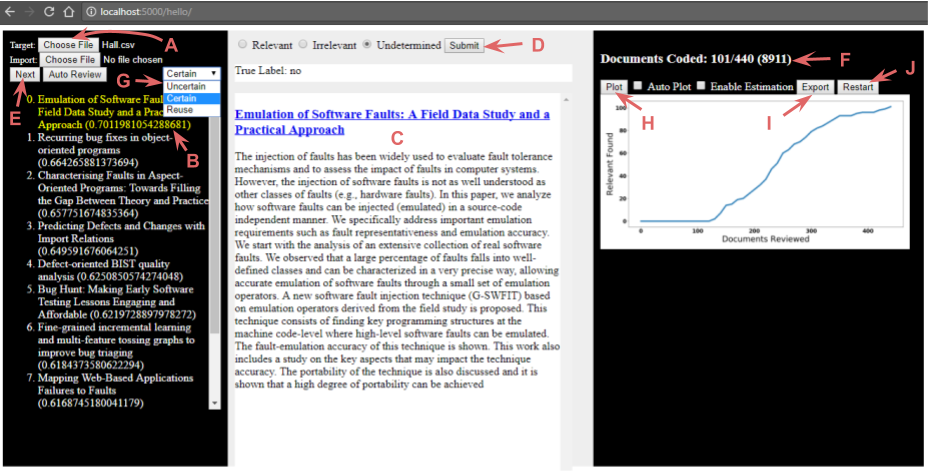
\includegraphics[width=\linewidth]{FASTREAD.png}
    \caption{Basic interface of the FASTREAD tool.}
    \label{fig:FASTREAD}
\end{figure*}


\begin{figure*}[!tbhp]
    \centering
    \subfloat[Input format]
    {
        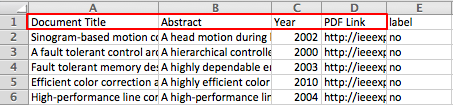
\includegraphics[width=0.48\linewidth]{Input.png}\label{fig:input}
    }
    \subfloat[Output format]
    {
        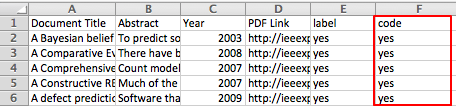
\includegraphics[width=0.48\linewidth]{Output.png}\label{fig:output}
    }    
    
    \caption{Data format for FASTREAD tool.}
    \label{fig:csv}
\end{figure*}

In order to implement FASTREAD, we developed a simple tool as shown in Fig.~\ref{fig:FASTREAD}. This software is freely available from SeaCraft Zenodo at \textit{https://doi.org/10.5281/zenodo.837861} and its Github repository at \textit{https://github.com/fastread/src}. 


Using FASTREAD, a review starts with \textbf{A}: selecting the input candidate study list from \textit{workspace/data/} directory. The input candidate list is specified in the format shown in Fig.~\ref{fig:input}. The input CSV file must have the \textit{Document Title}, \textit{Abstract}, \textit{Year}, and \textit{PDF Link} columns. The \textit{label} column, which is the true label of the candidate studies, is optional and is only used for testing. The output CSV file generated by the FASTREAD tool has an additional \textit{code} column, which is the reviewer-decided label for the candidate study. The final inclusion list can be retrieved by extracting all the studies with ``yes'' in the \textit{code} column.

The review then proceeds as follows:
\begin{enumerate}
\item[\textbf{B}] Randomly select $10$ candidate studies for review.
\item[\textbf{C}] Read through the title and abstract (and click on the title and read the full text if needed) of the candidate study.
\item[\textbf{D}] Decide whether this study should be coded as \textit{Relevant} or \textit{Irrelevant} and click the \textit{Submit} button.
\item[\textbf{E}] Click the \textit{Next} button and the codes are saved. Another $10$ candidate studies will be selected for review.
\item[\textbf{F}] The review status will change every time new studies are coded by reviewer and the \textit{Next} button is hit. The status is shown in the format ``Documents Coded: \textit{Number of relevant studies found} / \textit{Number of studies reviewed} (\textit{Total number of candidate studies}).''
\item[\textbf{G1}] Once \textbf{1} ``relevant'' study is coded, \textit{Random sampling} will be replaced by \textit{Uncertainty sampling}.
\item[\textbf{G2}] Once \textbf{30} ``relevant'' study is coded, \textit{Uncertainty sampling} can be changed to \textit{Certainty sampling}.
\item[\textbf{H}] Fig. can be plotted by clicking the \textit{Plot} button or checking \textit{Auto Plot}. The generated figure can also be found in the \textit{src/static/image/} directory. The new figure will overwrite any old one.
\item[\textbf{I}] Once finished, coded studies can be exported into a CSV file in the \textit{workspace/coded/} directory, in the format shown in Fig.~\ref{fig:output}.
\end{enumerate}

Note that the \textit{Restart} button (\textbf{J}) is only for testing and discards all codes.



\section{Threats to Validity}
\label{sect: Threats to Validity}

There are several validity threats to the design of this study~\cite{feldt2010validity}. Any conclusions made from this work must be considered with the following issues in mind:

{\em Conclusion validity} focuses on the significance of the treatment. To
enhance the conclusion validity of this work, we employed several statistical
tests (Scott-Knot) to reduce the changes of making spurious conclusions. 

{\em Internal validity} focuses on how sure we can be that the treatment
actually caused the outcome. To enhance our internal validity,
as far as possible, we heavily constrained our experiments
(see  our simulated in strictly controlled environments as discussed in Section~\ref{subsect: Controlled Variables}).

{\em Construct validity} focuses on the relation between the theory
behind the experiment and the observation. In this work, we evaluated
our results via different treatments with WSS@95 as stated in Section~\ref{subsect: Performance Metrics}-- note that those
measures took us as close as we can to computing
cost reduction without ``abstract relevant'' information. 
That is, it fits the objective of human-in-the-loop primary study selection as defined in the current literature~\cite{tredennick2015,cormack2015autonomy,cormack2014evaluation}. Increasing the number of different measures may increase construct validity
so, in future work, we will further explore more metrics.

{\em External validity }concerns how well the conclusion can be applied outside. All the conclusions in this study are drawn from the experiments running on three software engineering SLR datasets created with information from Hall, Wahono, Radjenovi{\'c} et al. studies~\cite{hall2012systematic,wahono2015systematic,radjenovic2013software} and one dataset provided by Kitchenham~\cite{kitchenham2010systematic}. Therefore, such conclusions may not be applicable to datasets of different scenarios, e.g., citation screening from evidence based medicine or TAR from e-discovery. Such bias threatens any classification experiment. The best any researcher can do is to document that bias then make available to the general research community all the materials used in a study (with the hope that other researchers will explore similar work on different datasets). Existing active learning techniques in citation screening have been criticized by Olorisade et al. for being not replicable~\cite{olorisade2016critical,olorisade2017reproducibility}. To this end, we have published all our code at \textit{https://github.com/fastread/src} and all our data at \textit{https://doi.org/10.5281/zenodo.837298}.

In the experiments, we assume that the human reviewer is always correct. In practice, this assumption cannot hold and problems such as disagreement between reviewers or concept drift (in which reviewers disagree with themselves as time passes) may occur.  As discussed
below when we discuss {\em Future Work}, we intend to explore this matter in the near future.

The comparisons in our experiment are based on the controlled variables listed in Section~\ref{subsect: Controlled Variables}. The conclusion in Section~\ref{subsect: Results} may become unreliable if any of the controlled variables changes.



\section{Conclusions}\label{sect: Conclusion}

Systematic literature reviews are the primary method for aggregating evidence in evidence-based software engineering. It is suggested for every researcher in software engineering to frequently conduct SLRs in~\cite{keele2007guidelines}. The hugest barrier to accomplish this is the cost. Usually an SLR would take months to finish and the conclusion drawn can be out of date in a few years. To tackle this barrier, this study focuses on primary study selection, one of the most difficult and time consuming steps in an SLR. Machine learning methods, especially active learning, are explored in our attempts to reduce the effort required to exclude primary studies. Three state-of-the-art active learning methods, two from evidence-based medicine and one from e-discovery, are analyzed and tested. In our experiments, we showed that by decomposing and reassembling the state-of-the-art treatments, a new treatment can be created which outperforms the state-of-the-art treatments and achieves a large cost reduction with 5\% recall lost.  

This work has lead to a simple software tool called FASTREAD, which
we described above in Section~\ref{sect: tool}. We are currently advertising
that tool on social media and hope that, very soon,
we will be  able to report on
case studies when other researchers use this tool. FASTREAD is
an open source tool, published in Github, and we also hope
that FASTREAD will be maintained and improved by numerous 
researchers exploring this kind of technology. 

\section{Future Work}
This study has several limitations as described in Section~\ref{sect: Frequently Asked Questions} and \ref{sect: Threats to Validity}. We plan to address those limitations in future work. Specific problems and plans for the future are listed below.

\begin{itemize}

\item
{\em Conclusions are drawn from three synthetic SLR datasets and one Kitchenham dataset.} Validate the generalizability of the results on different datasets, including datasets from evidence-based medicine and e-discovery.

\item
{\em Experiment results are evaluated by WSS@95, which assumes a stop rule of reaching 95\% recall.} How to stop at 95\% recall without first knowing the number ``relevant'' studies in the pool is an interesting topic. We are exploring this topic actively.

\item
{\em The size and prevalence of data can affect performance of FASTREAD.} The analysis of such effects may in return help estimate the prevalence, therefore makes it possible to estimate the total number of ``relevant'' studies in the pool.

\item
{\em About $10\%$ to $20\%$ efforts are spent on random selection step and most of the variances are also introduced in this step.} To speed up the random selection step, external expert knowledge will be introduced while unsupervised learning methods such as VTM or LDA will also be considered in future work. 

\item
{\em Some magic parameters are arbitrarily chosen, which may affect the performance.} However, parameter tuning is not a good fit for human-in-the-loop primary study selection because a) parameters should be tuned for the data working on; b) but the effect of applying different parameters can not be tested since querying extra label incurs extra cost. Therefore, novel methods should be explored for parameter selection; e.g. better criterion for when to switch from uncertainty sampling to certainty sampling (instead of the ``30'' relevant examples rule applied now).


\item
{\em Current scenario is restricted to having only one reviewer, which is impractical in practice.} Problems including how to assign review tasks to multiple reviewers and how to utilize reviewers with different cost and different capability will be explored in the future.

\item
{\em Current scenario assumes that reviewers never make mistakes, which is definitely not true in practice.} How to tackle concept drift (reviewers disagree with themselves) and how to settle disagreements (reviewers disagree with each other) would be valuable contributions for future work.

\item
{\em This study focuses only on primary study selection.} Assists on other steps of SLR such as searching, data extraction, and protocol development can also help reduce total effort of SLRs. The potential of combining VTM, snowballing, and other tools with FASTREAD needs to be explored as well.


\end{itemize}

 We invite other researchers to join us in the exploring the above. To that end, we have made all our tools and scripts readily available, on-line).

% With all the work in this study, a baseline result for human-in-the-loop primary study selection has now been established. There are still many concerns and potential improvements on FASTREAD, as discussed in Section~\ref{sect: Frequently Asked Questions}. We will keep working on the future work items and we believe that with all the materials in this work published, SE researchers can also explore further in SLR cost reduction. With our best hope, the effort required for conducting SLRs will eventually be reduced to days of work in the future and thus enable researchers to conduct SLRs much more frequently.

\section*{Acknowledgement}
The authors thank Barbara Kitchenham for
her attention to this work and for
sharing with us the ``Kitchenham'' dataset used in our experiments.
 
% \bibliographystyle{plain}
\bibliographystyle{spmpsci}
% \bibliography{sigproc} 
\documentclass{svjour3}
\usepackage{times}
\usepackage{blindtext, graphicx}

\usepackage{colortbl}
\usepackage{tikz}
\usepackage{microtype}
\def\firstcircle{(90:1.75cm) circle (2.5cm)}
\def\secondcircle{(210:1.75cm) circle (2.5cm)}
\def\thirdcircle{(330:1.75cm) circle (2.5cm)}
\smartqed

\usepackage{balance}
\definecolor{Gray}{rgb}{0.88,1,1}
\definecolor{Gray}{gray}{0.85}
\definecolor{lightgray}{gray}{0.8}
\setlength{\tabcolsep}{0.2em}


\usepackage{subfig} 



\usepackage{amsmath}
\DeclareMathOperator*{\argmin}{argmin}

\usepackage[framed]{ntheorem}
\usepackage{framed}
\usepackage{tikz}
\usetikzlibrary{shadows}
\theoremclass{Lesson}
\theoremstyle{break}

% inner sep=10pt,
\tikzstyle{thmbox} = [rectangle, rounded corners, draw=black,
fill=Gray!20,  drop shadow={fill=black, opacity=1}]
\newcommand\thmbox[1]{%
    \noindent\begin{tikzpicture}%w
    \node [thmbox] (box){%
        \begin{minipage}{.94\textwidth}%
        \vspace{-3mm}#1\vspace{-3mm}%
        \end{minipage}%
    };%
    \end{tikzpicture}}

\let\theoremframecommand\thmbox
\newshadedtheorem{lesson}{Finding}
\newcommand{\quart}[4]{\begin{picture}(80,4)%1
    {\color{black}\put(#3,2){\circle*{4}}\put(#1,2){\line(1,0){#2}}}\end{picture}}

\newcommand{\review}[1]{{\textit{#1}}~\\}
\newcommand{\todo}[1]{\textbf{\color{red}{#1}}}
\newcommand{\respto}[1]{
\fcolorbox{black}{black!15}{
\label{response:#1}
\bf
  \scriptsize R-{#1}}~
}
\newcommand{\citeresp}[1]{
{\bf (see } \fcolorbox{black}{black!15}{
 \bf
  \scriptsize R-{#1}}~{\bf{on page \pageref{response:#1})}}
}

%% space saving measures
% \usepackage[shortlabels]{enumitem}  
% \usepackage{url}

\begin{document}

\title{How to Read Less: On the Benefit of Active Learning for Primary Study Selection in Systematic Literature Reviews%\thanks{Grants or other notes
%about the article that should go on the front page should be
%placed here. General acknowledgments should be placed at the end of the article.}
}
% \subtitle{Do you have a subtitle?\\ If so, write it here}


% \pagenumbering{arabic} %XXX delete before submission

\author{Zhe Yu         \and
        Nicholas A. Kraft \and 
        Tim Menzies%etc.
}

%\authorrunning{Short form of author list} % if too long for running head

\institute{Zhe Yu \at
              Department of Computer Science, North Carolina State University, Raleigh, NC, USA \\
              \email{zyu9@ncsu.edu}           %  \\
%             \emph{Present address:} of F. Author  %  if needed
           \and
           Nicholas A. Kraft \at
              ABB Corporate Research, Raleigh, NC, USA\\
              \email{nicholas.a.kraft@us.abb.com}
            \and
           Tim Menzies \at
              Department of Computer Science, North Carolina State University, Raleigh, NC, USA \\
              \email{tim.menzies@gmail.com}
}

% \date{Received: date / Accepted: date}

\maketitle

\begin{abstract}
  
Systematic literature reviews (SLRs) are the primary method for aggregating and synthesizing evidence in evidence-based software engineering (SE). Primary study selection is a critical and time-consuming SLR step in which reviewers use
titles, abstracts, or even full texts to evaluate thousands of studies to find the dozens of them that are relevant to the research questions. We seek to reduce the effort of primary study selection in SE SLRs by exploring and refactoring the state-of-the-art active learning techniques from evidence-based medicine and legal electronic discovery. By refactoring those methods, we discovered FASTREAD, which is a new state-of-the-art in active learning for SE SLRs. When tested on four datasets generated from existing SE SLRs of Hall, Wahono, Radjenovi{\'c}, Kitchenham et al., FASTREAD outperformed the current state-of-the-art methods. Our results show that FASTREAD can save researchers much time during
 the literature review process (since they will need to review hundreds to thousands fewer abstracts ) 
 while sacrificing very little
in the final recall  (5\%).

\keywords{Active Learning\and Systematic Literature Review\and Software Engineering\and Primary Study Selection}

\end{abstract}



\section{Introduction}
\label{sect: Introduction}

The number of new publications every year is growing rapidly. For example, on defect
prediction, 729 studies were published on IEEE
Xplore\footnote{http://ieeexplore.ieee.org} during the year of 2005 while 1,564
studies were published during the year of 2015.
Given this increasingly faster pace of software engineering (SE) research,
it has become harder and harder to remain current with
the state-of-the-art research in software engineering.


\begin{figure*}[t]
    \centering
    \subfloat[Most Difficult Aspects of SLR Process.]
    {
        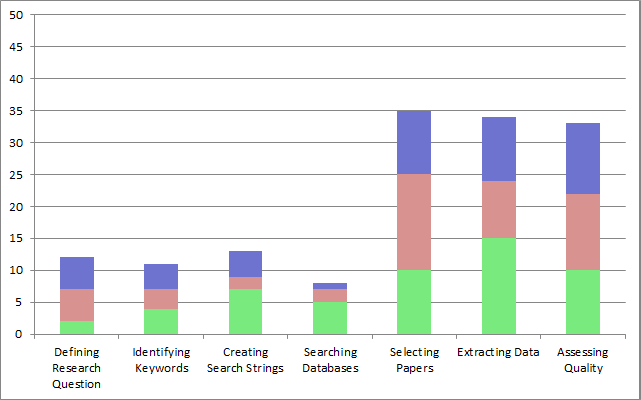
\includegraphics[width=0.48\linewidth]{difficulty.png}
        \label{fig: difficult}
    }
    \subfloat[Most Time Consuming Aspects of SLR Process.]
    {
        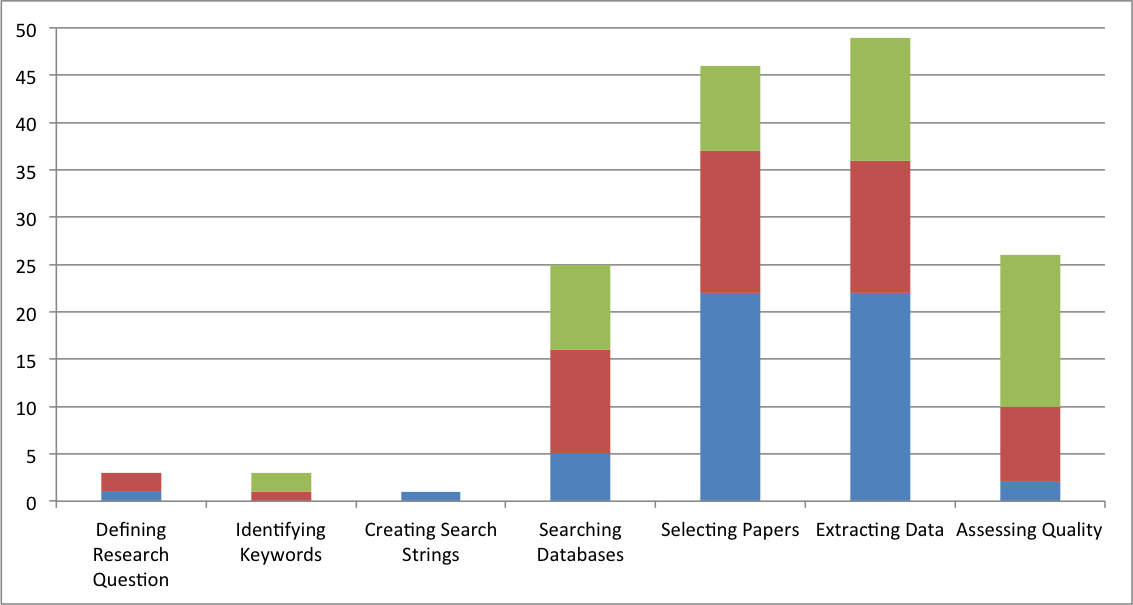
\includegraphics[width=0.48\linewidth]{time.png}
        \label{fig: time}
    }    
    \caption{Data collected from surveys to SLR authors~\cite{carver2013identifying}. Measured by number of votes, where {\setlength{\fboxsep}{1pt}\colorbox{green!40}{green}}, {\setlength{\fboxsep}{1pt}\colorbox{red!30}{red}}, and {\setlength{\fboxsep}{1pt}\colorbox{blue!50}{blue}} are number of times voted as most, second most, and third most, respectively.}
    \label{fig:barrier}
\end{figure*}
Systematic Literature Reviews
(SLRs) are one approach to this problem. SLRs are a well established and widely
applied review method in Software Engineering since Kitchenham, Dyb{\^{a}}, and
J{\o}rgensen first adopted it to support evidence-based software engineering in
2004 and 2005~\cite{kitchenham2004evidence,1377125}. 
Researchers can get a
general idea of current activity in their field of interests by reading the SLR
studies. Furthermore, a
deeper understanding of the topic may be gained by conducting an SLR.

An increasing number of SLRs has been conducted since the proposal and
revision of the SLR guidelines by Kitchenham in 2007~\cite{keele2007guidelines}. For
example, there were 26 SLRs on IEEE Xplore during the year of 2005 and that
number has increased to 137,199 for the years   2010,2015 (respectively). Various scholars  suggest that an SLR is required before any research in Software
Engineering is conducted~\cite{keele2007guidelines}.
While this is certainly a good advice,
currently an SLR is
a large, time consuming and complex
task~\cite{hassler2016identification,hassler2014outcomes,carver2013identifying,bowes2012slurp}.

Cost reduction in SLRs is therefore an important topic and will benefit researchers in software engineering community.
Previously we have analyzed the costs of SLRs~\cite{hassler2014outcomes,carver2013identifying}. As shown in Fig.~\ref{fig:barrier}, primary study selection, which is noted as ``selecting papers'' in Fig.~\ref{fig:barrier}, is among the top three most difficult
as well as time-consuming aspects in an SLR. Usually, reviewers need to evaluate
thousands of studies trying to find dozens of them that are relevant to the
research questions based on their title, abstract, or full text~\cite{bowes2012slurp}. An extreme
example of this is where reviewers sourced over
3,000 studies, and only used 7 of them in their final review~\cite{bezerra2009systematic}. The cost associated with primary study selection has become a serious problem and will continue to grow in the near future as the population of candidates for primary
studies increases dramatically. In this paper, we focus on reducing cost in primary study selection only. We prioritize primary study selection because there exists tool support for other time-consuming aspects such as searching databases~\cite{Molleri:2015:SWA:2745802.2745825,hernandes2012using}, extracting data\cite{Molleri:2015:SWA:2745802.2745825,hernandes2012using,fernandez2010slr,bowes2012slurp}, assessing quality~\cite{fernandez2010slr,bowes2012slurp,Molleri:2015:SWA:2745802.2745825}; and machine learning methods are promising in cost reduction for primary study selection~\cite{wallace2010semi,grossman2013}.

There are three main aspects in primary study selection: \textbf{(1)} retrieving initial list of primary studies, \textbf{(2)} excluding irrelevant studies, \textbf{(3)} including missing studies. We focus on excluding irrelevant studies because \textbf{a)} there already exists techniques and tools to facilitate \textbf{(1)} and \textbf{(3)} such as Snowballing~\cite{jalali2012systematic} and StArt~\cite{hernandes2012using}; \textbf{b)} the performance of excluding irrelevant studies can be evaluated using existing SLR publications.

In the SE research community, linear manual review, which requires reviewer to review every candidate study, is still the standard approach for primary study selection~\cite{kitchenham2013systematic}. On the other hand, machine learning algorithms, especially active learning, have been intensively studied to solve similar problems in other fields outside the SE research community in evidence-based medicine~\cite{paynter2016epc,wallace2010semi,wallace2010active} and in
legal electronic discovery~\cite{cormack2014evaluation,cormack2015autonomy}. This paper:
\begin{itemize}
\item
Reviews those methods. We find that in evidence-based medicine and legal electronic discovery, there are three widely recognized state-of-the-art active learning methods~\cite{cormack2014evaluation,wallace2010semi,miwa2014reducing}.
\item
Those three methods are assembled from four lower-level techniques including a) when to start training; b) query strategy; c) when/whether to stop training; d) data balancing. By analyzing techniques applied in the three methods, we generate 32 possible treatments.
\item
This paper explores all 32 treatments using data taken from the SE literature. Each treatment is evaluated by ``work saved over sampling at 95\% recall'' (WSS@95)~\cite{cohen2011performance}. 
\item
We find that one of those treatments, which we will call FASTREAD, robustly achieves the highest rank of performance across every dataset.
\end{itemize}
Interestingly, the FASTREAD treatment is not one of those used
in~\cite{cormack2014evaluation,wallace2010semi,miwa2014reducing}-- which is to say that the SE literature has nuanced differences to other kinds of literature and we should not just blindly
apply methods from other fields without certifying them on local data.
Using FASTREAD, hundreds to thousands of abstract reviewing can be avoided by sacrificing 5\% recall. That is, FASTREAD can dramatically reduce the cost of primary study selection in SE SLRs.

To assess those 32 treatments,
we need some ``gold sets'',
on which we can compare different combinations. Fortunately, in the arena of software engineering, there exist very prominent ``gold sets'' as published SLRs. This paper used three  primary study selection datasets by using the search strings and final inclusion list in such SLRs: Wahono et al. 2015~\cite{wahono2015systematic}, Hall et
al. 2012~\cite{hall2012systematic}, and Radjenovi{\'c} et al. ~\cite{radjenovic2013software}. These three SLRs are arbitrarily chosen from the set of SLR publications which define their work in enough details for us to construct datasets for simulations. Besides the three synthetic datasets, one set from Kitchenham et al. 2010~\cite{kitchenham2010systematic} has also been provided for the simulations. More details about the ``gold
sets'' will be presented later in Section~\ref{sect: datasets}. Using
these ``gold sets'', we ask and answer the following three research questions:

\begin{itemize}


\item
{\bf RQ1: Can active learning techniques reduce cost in primary study selection?} First of all, the effectiveness of active learning should be tested against traditional linear review. The rest of the research questions should not be investigated until active learning has been proved to be useful for cost reduction in primary study selection.

\item
{\bf RQ2: Should we just adopt the state-of-the-art treatments from other fields? Is it possible to build a better one by mixing and matching from those?} Active learning methods have been explored in other fields. Each of the state-of-the-art methods has its own advantage and thereby a better method might be derived by mixing and matching from those. 

\item
{\bf RQ3: How much effort can FASTREAD, our new state-of-the-art method for primary study selection, save in an SLR?} Details should be provided so that reviewers can decide whether to use FASTREAD or not.


\end{itemize}
The main contributions of this paper are:
\begin{itemize}
\item
  A demonstration of the value of  machine learning techniques for assisting primary study selection in SE SLRs.
\item
  The development of FASTREAD, a new state-of-the-art active learning method for primary study selection in SE SLRs, by refactoring three state-of-the-art methods from evidence-based medicine and electronic discovery.
  
\item
  The evaluation of our new method. The experiments shown below indicate that FASTREAD saves large amount of review efforts on primary study selection.
\item The development of a simple tool to implement FASTREAD for primary study selection.
  This tool is explained in Section~\ref{sect: tool} and is
  available for download on GitHub\footnote{https://github.com/fastread/src}. 
\end{itemize}










\section{Frequently Asked Questions}
\label{sect: Frequently Asked Questions}

When we discuss FASTREAD with our colleagues, several issues are commonly raised. This section discusses these issues.

\subsection{What about the other costs associated with SLRs?}

Our focus on the cost reductions of primary study selection is not to discount the effort associated with other parts of the SLR process. As mentioned in our introduction, we focus here on primary study selection since our data (from Fig.~\ref{fig:barrier}) indicates that this is a major component of SLR cost. 

In addition, there are tools support other components of SLRs and techniques facilitating primary study selection in different approaches. All these techniques (such as Quasi-Gold Standard based search~\cite{zhang2011empirical,zhang2011identifying}, visual text mining~\cite{Felizardo:2014:VAA:2601248.2601252,felizardo2012visual,felizardo2010approach,malheiros2007visual}, and snowballing~\cite{wohlin2014guidelines,jalali2012systematic}) are compatible and a better performance is expected when applied together. This leads to a direction of future work in which the best setting to integrate different techniques will be explored.

\subsection{What is missed?}

Our results will show, with FASTREAD, $95\%$ of the ``relevant'' studies can be retrieved by reviewing a small portion (usually hundreds of studies) of long candidate study list. Given that, it is wise to reflect
on the 5\% of papers {\em not} found by such an analysis. To this end, we took one of our case studies and reflected on:
\begin{itemize}
\item The set of papers $P_0$ that a human analyst declared to be ``relevant'' (as listed in their reference list at the end of their paper);
\item The {\em tangentially relevant} subset of those  papers $P_1 \subseteq P_0$ that a human analyst explicitly mentions, however briefly, in the body of their paper;
\item The yet smaller subset of those papers $P_2 \subseteq P_1$  that a human analyst discusses, at length, in the body of their report (and for
our purposes ``at length'' will be ``more that two lines''). We call these {\em insightful papers}. Clearly, FASTREAD should not be recommended if our method always misses the insightful papers, 
\end{itemize}
For the case studies shown below, on 30 repeats of our methods, we found that $|P_2|=0$; i.e. FASTREAD never missed an insightful paper. As for the tangentially
relevant papers, FASTREAD found all of those in 95\% of the 30 repeats. 
Based on this analysis, we infer that missing  $15\%$ of the papers is not a major impediment to using FASTREAD. Similar conclusion was derived by Shemilt et al. in 2016~\cite{shemilt2016use}.

That said, it is still true that if the SLR conductor does not want to miss any potential relevant study, he or she need to review all the candidate studies with full cost. We are actively exploring possibilities to mitigate or compensate the missing studies issue. 

% Data imbalance is explored further in Fioravanti and Nesi
% [[43]] and Zhang et al..

% Nikora and Munson [[126]] says that “without a widely agreed definition of severity
% we cannot reason about it” and Ostrand et al.
 

\subsection{What about domain knowledge?}

In our simulations, we assume that no initial seed training set is available thus a random sampling is performed to collect the minimum training set. This assumption represents the worst case while no external knowledge is available. We show in this work that the absence of that domain knowledge is not a critical failing of the approach. On the other hand, such domain knowledge usually exists in real world SLRs and will boost the performance of FASTREAD if wisely used. For example, if one relevant example and one irrelevant example are known in the very beginning, the random sampling step of FASTREAD is no longer needed and thus leads to additional cost reduction. More details about how to wisely use domain knowledge to boost FASTREAD will be explored further after this work. While we have some preliminary results in that area, we have nothing definitive to report at this time.

\subsection{What about real human reviewers?}

In our simulations, we assume that there is only one reviewer who never make mistakes. In real world SLRs, there will be multiple reviewers who make some mistakes. 

First, consider we have multiple reviewers but no mistakes. The schema of FASTREAD can be changed to one central learner with multiple review agents. Every agent reviews different studies and feedback his or her decisions to the central learner. The central learner then trains on the feedback of every agent and assigns studies to each agent for review. Such schema will keep all the property of single reviewer FASTREAD and performs similarly. In addition, there might be more intelligent way to allocate review tasks based on the different performance of review agents. Such possibility is worth exploring in future works and there already exists some studies on this topic in evidence-based medicine~\cite{wallace2011should}.

Second, consider those multiple reviewers now make mistakes. Candidate studies need to be reviewed by multiple reviewers in case any of them makes mistakes. To explore this issue, appropriate data need to be collected on how human reviewers make mistakes. Wallace et al. addressed this issue in~\cite{nguyen2015combining} by analyzing the best policy for allocating review tasks to reviewers with different experience levels as well as difference costs. We also plan to to address this issue in our future work.


\subsection{What about multiple categories of studies?}

In our simulations, we assume that the target is binary classification. However, primary study selection in real world SLRs might be a multi-label classification problem. For example, an SLR with two research questions might go through a primary study selection while each candidate is labeled as ``relevant to RQ1'', ``relevant to RQ2'', or ``irrelevant'' while the first two labels can co-exist. The simplest solution for this is to run multiple FASTREAD learners each learns on one label vs. others and each reviewer classify on one label only. In this case, the multi-label classification problem can be divided into multiple FASTREAD problems. Additional work such as ensemble learners can be explored in future works.

In summary, FASTREAD is an in-development technique that can be applied if the above trade-offs are acceptable. It can still be improved to further reduce cost of primary study selection and we will keep working on the issues until it becomes a reliable tool for different scenarios of SLRs.

























\section{Large Scale Literature Studies in SE}
\label{sect: Background}

\begin{figure}[t]
    \centering
    \begin{minipage}[t]{.51\linewidth}
    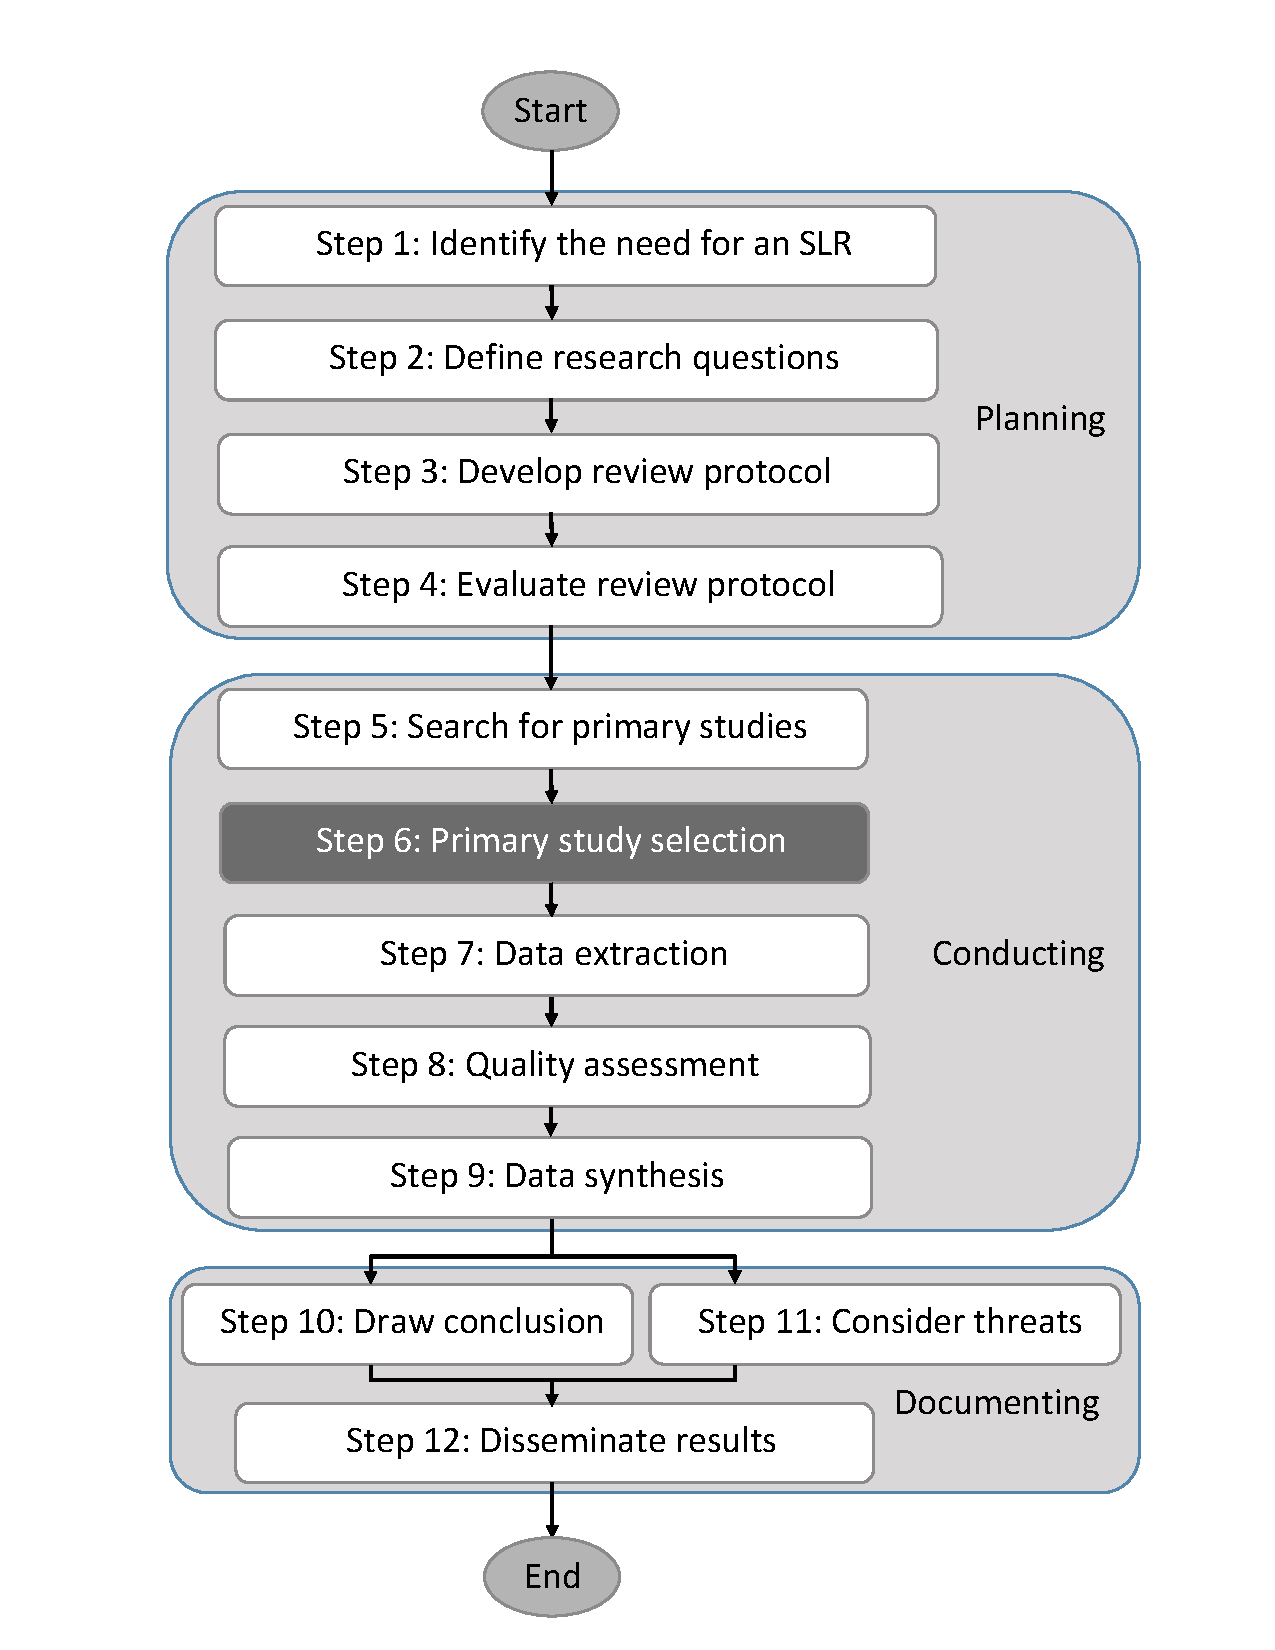
\includegraphics[width=\linewidth]{procedure.pdf}
    \caption{Systematic literature review steps suggested by~\cite{keele2007guidelines}. In this work, we focus on Step 6: primary study selection.}
    \label{fig: slr}
    \end{minipage}\quad
    \begin{minipage}[t]{.45\linewidth}
    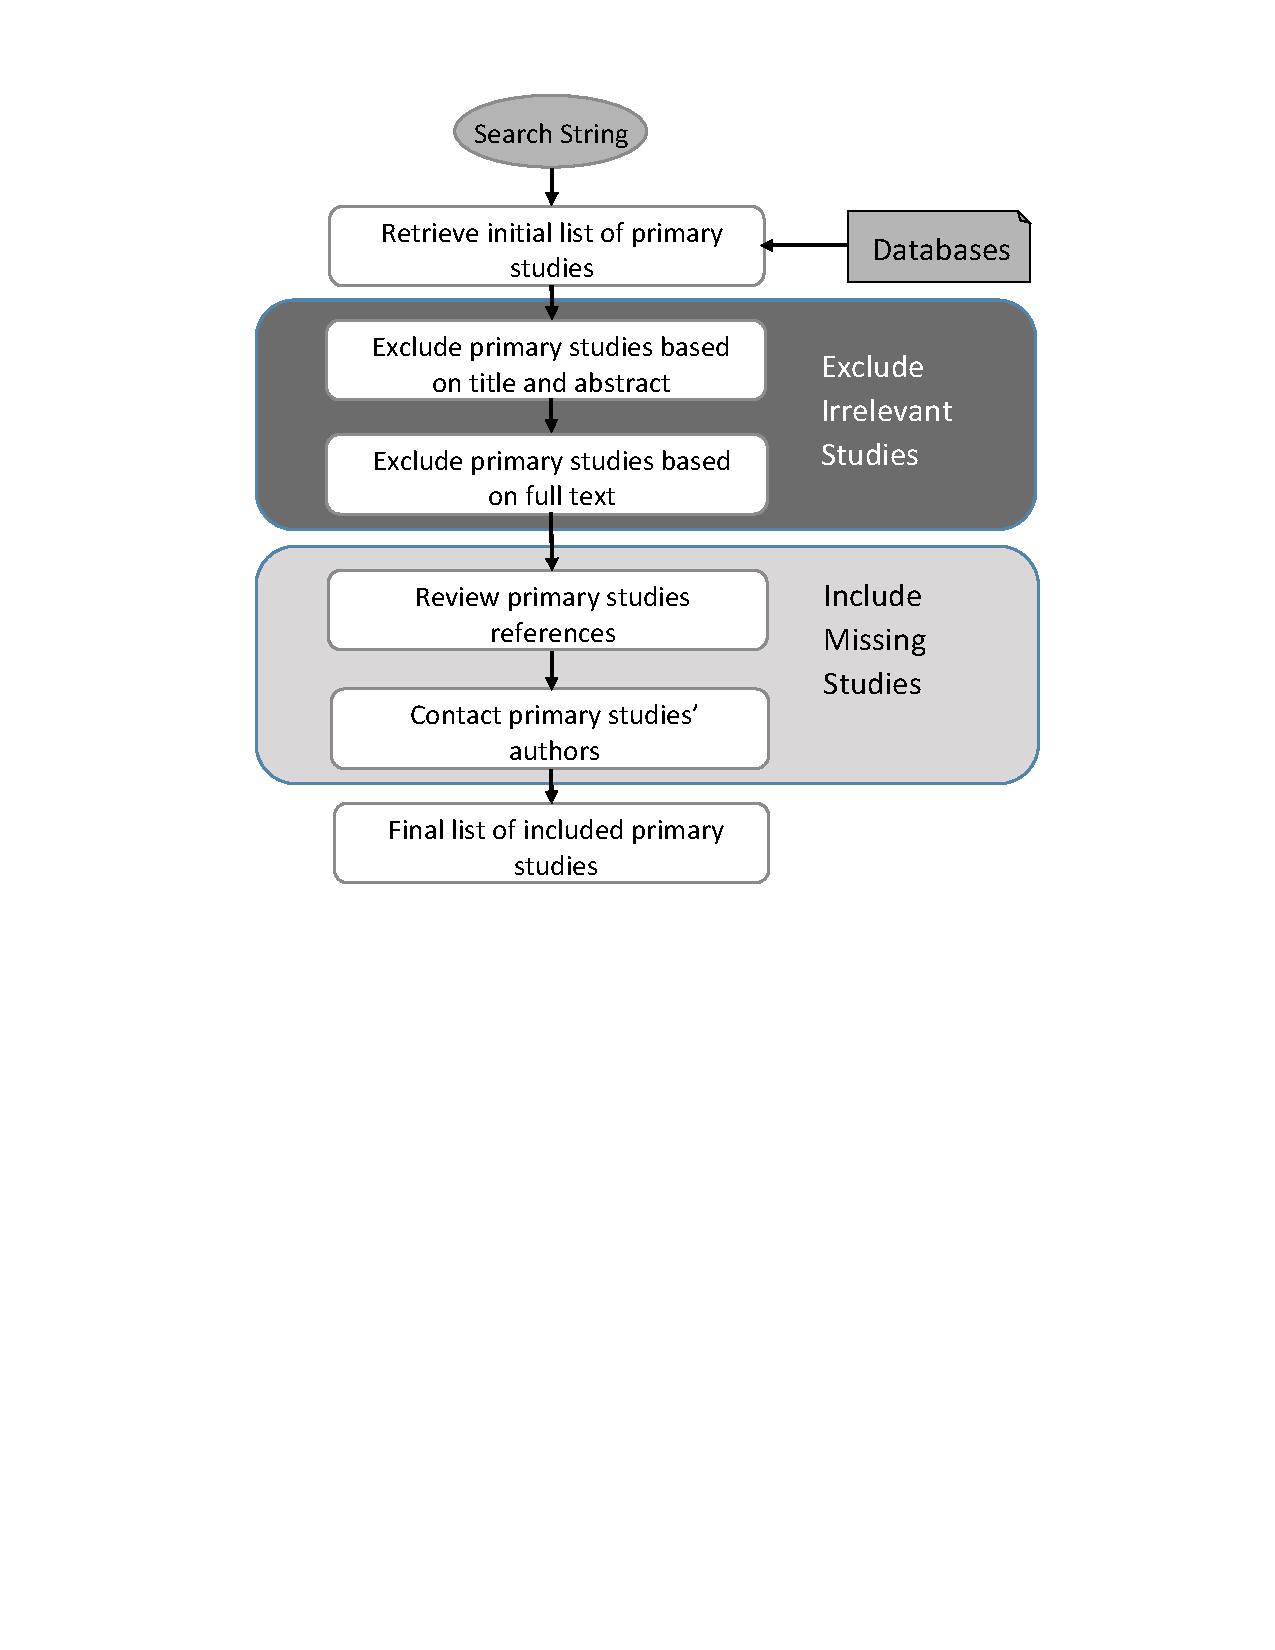
\includegraphics[width=\linewidth]{primary_study_selection.pdf}
    \caption{Primary study selection steps suggested by~\cite{keele2007guidelines}. In this work, we focus on the excluding irrelevant studies part.}
    \label{fig: prime}
    \end{minipage}
\end{figure}



% In contrast to a primary study, which investigates a specific research question,
% a systematic literature review is a form of secondary study aimed at
% identifying, evaluating and interpreting all available research relevant to a
% particular research question, topic area, or phenomenon of
% interest~\cite{keele2007guidelines}.
In the modern academic world, it is
impossible to start research without first knowing what other researchers have
done in the topic area. Conducting an SLR is one way to gain
background knowledge on a certain topic area.
If that SLR is published, then that paper becomes a useful research tool
for other researchers.  Kitchenham recommend SLRs to be standard
procedure in SE research~\cite{kitchenham2004evidence,keele2007guidelines}.

An SLR is usually conducted following the procedures in Fig.~\ref{fig: slr}. There can be variances on the real
implementations~\cite{wahono2015systematic,malhotra2015systematic,radjenovic2013software,unterkalmsteiner2012evaluation,hall2012systematic},
but all are based on the same guideline~\cite{keele2007guidelines}. Among all these steps, primary study selection is an important early step in SLRs. It starts with an initial candidate collection of studies retrieved by searching. In the first round of that process,
the reviewers' job is to read the titles and abstracts of candidate studies and classify each as ``relevant'' or ``irrelevant''. After the first round of review, the reviewers read through the full text of the previously included studies and make further decision on whether it is actually ``relevant'' or not. The whole procedure is shown in Fig.~\ref{fig: prime}. Typically, reviewers need to identify a final list of dozens of primary studies
among the initial collection of thousands of candidates. In terms of actual
cost, Malheiros has documented in~\cite{malheiros2007visual} that it requires 3
hours for one reviewer to review 100 studies.  This implies that it is a month's
work for one graduate student to review 3000 studies or three months' work to
review 9000 studies. 

In this work, we try to reduce the cost of the primary study selection by applying machine learning techniques to assist excluding irrelevant studies. In our {\em active learning} approach, each time a human reviews a paper, a learner updates its knowledge about what kind of documents are relevant. After that, the human uses that learned knowledge to guide the selection of the next paper to read.

The review cost of primary study selection can not be simply measured by the number of studies reviewed since the effort required for content review ($C_D$) is much higher than that for abstract review ($C_A$). Suppose one review process first identified $N_A$ ``relevant'' studies via reviewing $N$ abstracts, then reviewed the content of the $N_A$ studies and found $N_D$ of them are ``content relevant''. That is, to retrieve the $N_D$ ``content relevant'' studies, a total review cost of $C=N\times C_A+N_A\times C_D$ is required. To calculate this review cost, two level of relevance information is required (labels for ``abstract relevant'' and labels for ``content relevant''). However, most datasets of systematic literature review (including three datasets used in this study) have only one level of relevance information. As a result, only $N$ is used for review cost estimation since $N_A$ is not available. While this could be a fair metrics for comparing different treatments (smaller $N$ reflects less review cost in general), it is not a good estimation for how much effort saved by the text mining technique. Fortunately, the Kitchenham dataset provides two level of relevance information and we will explore the detailed review cost on this dataset in RQ3.





\subsection{Semi-Automated Tools for Literature  Reviews}

\subsubsection{Software Engineering Tools}

In recent years, various tools have been developed to facilitate SLRs in software engineering community, as summarized in~\cite{marshall2015tools,marshall2014tools,marshall2013tools}. These tools aim at providing support for protocol development~\cite{Molleri:2015:SWA:2745802.2745825,fernandez2010slr,hernandes2012using}, automated search~\cite{Molleri:2015:SWA:2745802.2745825,hernandes2012using}, primary study selection~\cite{Molleri:2015:SWA:2745802.2745825,hernandes2012using,fernandez2010slr,bowes2012slurp}, quality assessment~\cite{fernandez2010slr,bowes2012slurp,Molleri:2015:SWA:2745802.2745825}, data extraction and validation~\cite{Molleri:2015:SWA:2745802.2745825,hernandes2012using,fernandez2010slr,bowes2012slurp}, data synthesis~\cite{Molleri:2015:SWA:2745802.2745825,hernandes2012using,fernandez2010slr,bowes2012slurp},
and report write up~\cite{Molleri:2015:SWA:2745802.2745825,hernandes2012using,fernandez2010slr,bowes2012slurp}. It is extremely helpful to have a tool for managing the whole SLR process. However, the support for primary study selection using these tools is limited (e.g., to tasks such as assigning review jobs to multiple reviewers or to resolving disagreements).
Hence, we assert that the current SE SLR literature provides
no tool that can offer reductions in the effort required for primary study selection comparable to those reductions offered by active learning. Note that existing tools from Evidence-based Medicine offer active learning support and will be discussed in Section~\ref{sect: Evidence-based Medicine}.

Visual text mining (VTM) is a technique especially explored in Software Engineering community to support SLR. It is an unsupervised learning method which visualizes the relationship between candidate studies and helps the reviewer to make quick decisions. Malheiros et al.~\cite{malheiros2007visual} first applied VTM to support primary study selection in SLR. In their small-scale experiment (100 candidate studies, 31 of which are ``relevant''), VTM retrieves around 90\% of the ``relevant'' studies by spending about 30\% as much time as manual review. However, VTM requires some prior experience and knowledge of text mining and visualization techniques to use~\cite{bowes2012slurp}, and more case studies with large scale are needed to validate their results. 


Snowballing is another technique attracting much attention in SE SLR research. Given the inherent relevance relationship between a study and its citations, it is of high probability for the citations of (used in backward snowballing) and the studies cite (used in forward snowballing) a known ``relevant'' study to also be ``relevant''~\cite{kitchenham2004evidence}. Jalali and Wohlin~\cite{jalali2012systematic,wohlin2014guidelines} applied backward snowballing to search for primary studies in SE SLRs and found comparably good result as database search. Felizardo et al.~\cite{felizardo2016using} and Wohlin~\cite{wohlin2016second} applied forward snowballing to update SE SLRs and greatly reduced the number studies need to be reviewed comparing to a database search. This paper does not use snowballing since, as mentioned by Wohlin~\cite{wohlin2014guidelines}, snowballing starts with an initial set of relevant papers.
FASTREAD's task is very different: we start with zero relevant papers.



\subsubsection{Legal Electronic Discovery Tools}
\label{sect: Electronic Discovery}

Electronic Discovery (e-discovery) is a part of civil litigation where one party (the producing party), offers up materials which are pertinent to a legal case~\cite{krishna2016bigse}. This involves a review task where the producing party need to retrieve every ``relevant'' document in their possession and turn them over to the requesting party. It is extremely important to reduce the review cost in e-discovery since in a common case, the producing party will need to retrieve thousands of ``relevant'' documents among millions of candidates. Technology-assisted review (TAR) is the technique to facilitate the review process. The objective of TAR is to find as many
of the ``relevant'' documents in a collection as possible, with reasonable cost~\cite{grossman2013}. Various machine learning algorithms have been studied in TAR. So far, in every controlled studies, continuous active learning has outperformed others~\cite{cormack2014evaluation,cormack2015autonomy}, which makes it the state-of-the-art method in legal electronic discovery. It has also been selected as a baseline method in the total recall track of TREC 2015~\cite{roegiest2015trec}. Details on continuous active learning will be provided in Section~\ref{sect: Continuous Active Learning}. 

% Interestingly, the relationship between e-discovery and evidence-based medicine have been discussed in~\cite{leasesystematic} but their methods are still diverged. Relying on Grossman and Cormack~\cite{grossman2013} for support, many legal service providers have adopted TAR to facilitate the review process.

% In summary: the state-of-the-art active learning techniques are patient active learning in evidence-based medicine and continuous active learning in e-discovery.

\subsubsection{Evidence-based Medicine Tools}
\label{sect: Evidence-based Medicine}

Systematic literature reviews were first adopted from evidence-based medicine in
2004~\cite{kitchenham2004evidence}. To facilitate citation screening (primary
study selection) in systematic review, many groups of researchers have investigated different types of machine learning algorithms and evaluation mechanisms~\cite{o2015using,paynter2016epc}. 

Cohen et al. first applied text mining techniques to support citation screening and developed several performance metrics (including WSS) for assessing the performance of different techniques in 2006~\cite{cohen2006reducing}. While the great contribution of introducing machine learning and text mining into citation screening as well as the proposed performance metrics of Cohen has been widely acknowledged~\cite{o2015using}, most of Cohen's work focused on supervised learning which does not utilize unlabeled data and relies on random sampling to obtain the sufficiently large training set~\cite{cohen2006reducing,cohen2006effective,cohen2010prospective,cohen2011performance}.

Wallace et al. conducted a series of studies
with machine learning techniques, especially active
learning~\cite{wallace2010semi,wallace2010active,wallace2011should,wallace2012deploying,wallace2013active,wallace2013modernizing,nguyen2015combining}. Wallace
first set up a baseline approach called ``patient active learning'' (PAL), which will be explained later in this subsection, for machine learning assisted citation screening~\cite{wallace2010semi}. The performance of patient active learning is good enough (nearly 100\% of the ``relevant''
citations can be retrieved at half of the conventional review cost) to convince
systematic review conductors to adopt machine learning assisted citation
screening. Instead of improving this baseline method, Wallace then focused on other aspects of machine learning assisted citation screening such as introducing external expert knowledge~\cite{wallace2010active}, allocating review tasks to multiple experts~\cite{wallace2011should} or to crowdsourcing workers~\cite{nguyen2015combining}, and building a tool called abstrackr to provide overall support~\cite{wallace2012deploying}. Wallace's work on this topic is of exemplary high-impact and his core algorithm   (on simple expert screening),   is one of the most popular active learning techniques we have found in the evidence-based medical literature. That said, this technique has not been updated since 2010~\cite{wallace2010semi}. In this paper we are focused on the core active learning algorithm for cost minimization. Hence, we do not explore techniques such as Wallace's use of multiple experts (but in future work, we will explore this approach).

More recent work of Miva et al. explored alternative data balancing and query strategy in 2014~\cite{miwa2014reducing} and proposed a new treatment of Certainty plus Weighting. Instead of uncertainty sampling in PAL (and most conventional active learning approaches), Miva found that certainty sampling provides better results in clinical citation screening tasks. Similar conclusion for data balancing method as weighting relevant examples was found to be more effective than aggressive undersampling. Although not stated explicitly, Certainty plus Weighting keeps training until all ``relevant'' studies have been discovered, which differs from the stopping criteria of PAL. Aside from the core algorithm, additional views from latent Dirichlet allocation (LDA) has been found to be potentially useful.

Other work related to machine learning assisted citation screening do not
utilize active learning and active learning. Pure supervised learning requires a sufficiently large training set, which leads to a huge review cost~\cite{cohen2006reducing,adeva2014automatic}. Semi-supervised learning~\cite{liu2016comparative} does not utilize the human reviewers' feedback for updating the model, which leads to a depreciated performance in a long run. As a result, the patient active
learning proposed by Wallace et al.~\cite{wallace2010semi} and the Certainty plus Weighting approach by Miwa et al.~\cite{miwa2014reducing} are still considered to be the state-of-the-art method for citation screening in the scenario with no external knowledge and equally expensive reviewers. Details on these two approaches will be provided in Section~\ref{sect: Patient Active Learning} and \ref{sect: Certainty plus Weighting}.

There are also existing tools to support study selection in systematic reviews, e.g. Abstrakr\footnote{http://abstrackr.cebm.brown.edu}~\cite{wallace2012deploying}, EPPI-Reviewer\footnote{http://eppi.ioe.ac.uk/cms/er4/}~\cite{thomas2010eppi}, Rayaan\footnote{http://rayyan.qcri.org/}~\cite{Ouzzani2016}. Amazing features can be found in these tools such as a) Rayaan and EPPI-Reviewer: incorporated keyword search in screening; b) Rayaan and EPPI-Reviewer: deduplication; c) Rayaan and EPPI-Reviewer: define inclusion/exclusion criteria by terms; d) Abstrakr: user defined tags; e) all three: assign review tasks to multiple reviewers; f) all three: automatically extract data from PubMed. However, the active learning parts alone in these tools are depreciated. Under the condition that no additional feature (search, tags, define inclusion/exclusion terms) is used, we tried all three tools with one of our dataset-- Hall set (106 relevant in 8911 studies) and after reviewing 1000 studies, only 10 to 15 relevant ones were found, which was very close to a random sampling result without any learning. Since none of these tools are open-source, we cannot tell whether active learning is applied or how/when it is applied in each tool. This motivates us to develop an open source tool which focuses on active learning to support the primary study selection process. Details about our tool will be presented in Section~\ref{sect: tool}.



\section{Technical Notes}
\label{sect: Technical Briefing}

\begin{figure}[!t]
    \centering
    \subfloat[SVM without data balancing]
    {
        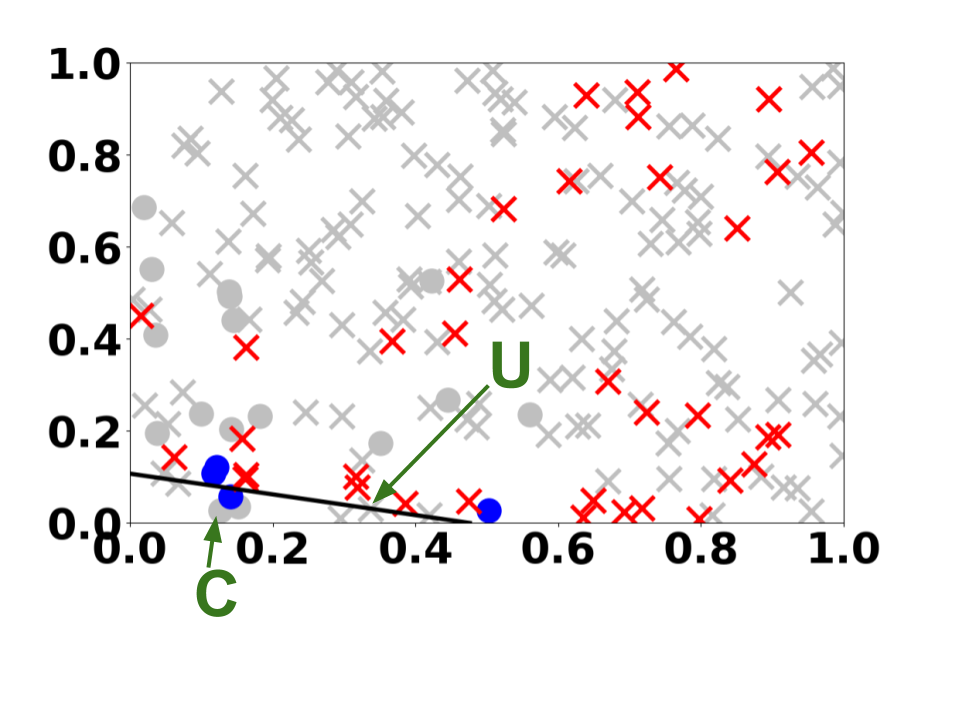
\includegraphics[width=0.3\linewidth]{simu22.png}
        \label{fig:train}
    }
    \subfloat[SVM with aggressive undersampling]
    {
        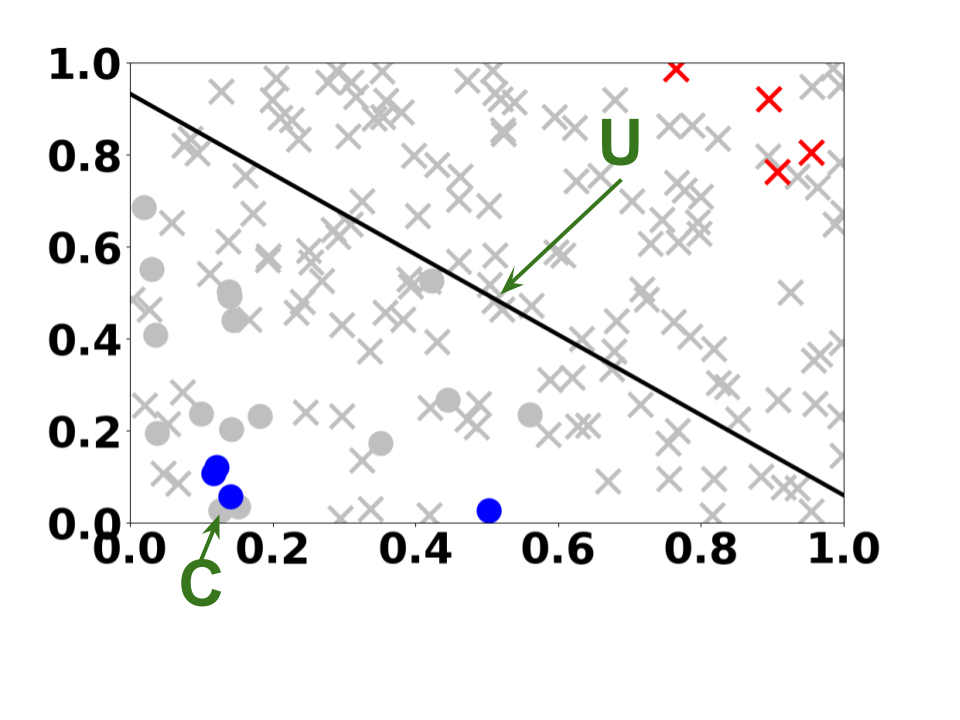
\includegraphics[width=0.3\linewidth]{simu23.png}
        \label{fig:train_a}
    }
    \subfloat[SVM with Weighting]
    {
        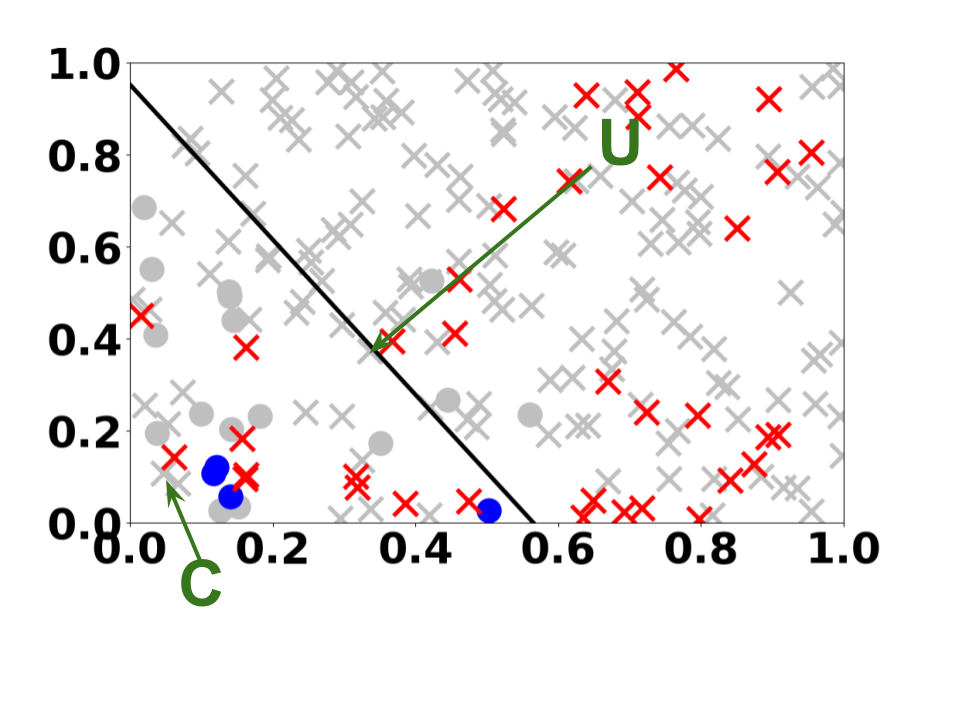
\includegraphics[width=0.3\linewidth]{simu24.png}
        \label{fig:test}
    }

    \caption{A demonstration of how SVM model is trained on imbalanced data, where ``$O$'' is the minority class, ``relevant'' studies in SLR, ``$X$'' is the majority class, ``irrelevant'' studies in SLR, markers in gray are the unlabeled studies, and black line is SVM decision plane. In (b), aggressive undersampling balances the training data by throwing away majority class examples closest to the old decision plane in (a). In (c) Weighting balances the training data by putting more weight on the minority class examples. Uncertainty sampling returns the unlabeled examples closest to the decision plane while certainty sampling returns the unlabeled examples furthest to the decision plane from the bottom-left side.}
    \label{fig:SVM}
\end{figure}

In this section, we provide details on technical terms 
used in the paper,  along with some brief introductory
notes on machine learning techniques used in this study.


\subsection{Linear Review}
\label{sect: Linear Review}

Linear review lets the reviewer to review and label every candidate study in a random order. This is still the most popular review method when there is unlimited review budget and completeness is the major objective. In this study, linear review works as a baseline method where no text mining technique is applied.

\subsection{Support Vector Machine}
\label{sect: Support Vector Machine}

Support vector machines (SVM) are a well-known and widely used classification method. The idea behind is to map input data to a high-dimension feature space and then construct a linear decision plane in that feature space~\cite{cortes1995support}. Linear SVM~\cite{joachims2006training} has been proved to be a useful model in SE text mining~\cite{krishna2016bigse} and is applied in the state-of-the-art active learning methods of both evidence-based medicine and electronic discovery~\cite{miwa2014reducing,wallace2010semi,cormack2014evaluation}. Fig.~\ref{fig:SVM} illustrates how linear SVM model is trained on a two-dimension feature space with different data balancing techniques.

\subsection{Active Learning}
\label{sect: Active learning}

Active learning is a cost-aware machine learning algorithm where labels of training data can be acquired with certain costs. The key idea behind active learning is that a machine learning algorithm can perform better with less
training if it is allowed to choose the data from which it learns~\cite{settles2012active}. There are several scenarios active learning is applied to, such as membership query synthesis, stream-based selective sampling, and pool-based sampling~\cite{settles2010active}. There are also different query strategies of active learning, such as uncertainty sampling, query-by-committee, expected model change, expected error reduction, variance reduction, and density-weighted methods~\cite{settles2010active}. Here, we will briefly introduce one scenario and two query strategies, which will be used in our later experiments and discussions.

\textbf{Pool-based sampling} is the scenario of primary study selection. This scenario starts with a fixed size pool of unlabeled data. Labels for the data can be acquired by querying an oracle selectively. The goal of pool-based sampling is to select the most informative data in the pool for query, thereby building a better model with less training.

\textbf{Uncertainty sampling} is the query strategy utilized in the state-of-the-art active learning technique of evidence-based medicine~\cite{wallace2010semi,wallace2010active}. It is also recognized as the most simple and commonly used query strategy~\cite{settles2010active}. In this query strategy, uncertainty sampling queries the instances about which the learner is least certain how to label. These instances are those (a) whose posterior probability of being positive are nearest 0.5 in probabilistic models or (b) closest to the decision boundary in models such as SVM. 

\textbf{Certainty sampling} is another query strategy which is applied in the state-of-the-art active learning technique of electronic discovery~\cite{cormack2014evaluation,cormack2015autonomy} and is also preferred over uncertainty sampling by Miwa et al. \cite{miwa2014reducing}. In contrast to uncertainty sampling, certainty sampling queries the instances about which the learner is most certain to label as positive. These instances are those (a) whose posterior probability of being positive are highest in probabilistic models, or (b) lies in the positive side of the decision boundary and furthest to the decision boundary in models such as SVM. This query strategy is usually NOT used when building the classifier of active learning since it is commonly believed that examples queried by certainty sampling contains less information than those by uncertainty sampling.

% \subsection{active Learning}
% \label{sect: active Learning}

% active learning is a combination of human decisions and machine
% suggestions~\cite{tredennick2015}. In this approach:
% \begin{itemize}
% \item
% Humans read a stream of documents, commenting on whether or
% not each one is ``relevant''.
% \item
%   Machine learners use feedback from the human opinion to
%   incrementally update their models actively.
% \item
%   The models generated via machine learning are used
%   to sort the stream of documents such that the humans focus on the
%   most informative documents.
%   \end{itemize}

% This is a
% pool-based active learning scenario since \textbf{a)} the process starts with a fixed size candidate list without any labels and \textbf{b)} training examples gradually become available to the learner as the human reviewer reviews the documents.  However, an important difference between active learning and other active learning methods is that every document labeled as ``relevant'' has been reviewed by a human. The machine never makes the final decision on whether a document is ``relevant''; a human makes such decisions and the machine only suggests a review order based on the human input. As a result, instead of building a better classification model, the objective of active learning is to retrieve most ``relevant'' documents from a pool of candidates while manually reviewing as few documents as possible. 

% Simple active learning, which is pool-based active learning with uncertainty sampling~\cite{settles2012active}, is the most basic form of learning methods
% applied to active learning. Although simple active learning achieves
% satisfactory performance, it has been outperformed by the state-of-the-art active learning techniques in both evidence-based medicine~\cite{wallace2010semi} and electronic discovery~\cite{cormack2014evaluation}. 


\subsection{Patient Active Learning}
\label{sect: Patient Active Learning}

One of the state-of-the-art active learning method in evidence-based medicine, patient active learning (PAL) can be described as following~\cite{wallace2010semi}:

\begin{itemize}

\item
{\bf Stage I: Construct an initial seed training set} by randomly sampling from the candidate study pool and asking a human reviewer to label the sampled papers as ``relevant'' or ``irrelevant''. Stop and proceed to Stage II when \textit{enough} ``relevant'' studies have been retrieved to represent the ``relevant'' class. (Note that Wallace et al.~\cite{wallace2010semi} did not provide an explicit definition of \textit{``enough''}.)

\item
{\bf Stage II: Build the classifier}, which is a linear SVM, by repeatedly training on labeled studies and uncertainty sampling. Unlabeled studies in the pool will be ranked in the descending order of uncertainty (uncertainty sampling). The human reviewer labels the studies in the ranked order and feeds them back to retrain the classifier. Stop and proceed to Stage III when the classifier is \textit{stable}. (Note that Wallace et al.~\cite{wallace2010semi} did not provide an explicit definition of \textit{``stable''}.)

\item
{\bf Stage III: Prediction.} Retrain the classifier with \textbf{aggressive undersampling} and then stop training. Unlabeled studies in the pool will be ranked in the descending order of the classifier's prediction probability of being ``relevant'' (certainty sampling as discussed in Section~\ref{sect: Active learning}). The human reviewer labels the studies in the ranked order until finished (running out of review cost budget, enough ``relevant'' studies found, or no more ``relevant'' studies are detected in multiple rounds).

\end{itemize}

{\bf Aggressive undersampling: }The data for citation screening are (at times, extremely) imbalanced, i.e., the prevalence of ``relevant'' citations is always smaller than $50\%$ (and often much smaller). Classification algorithms are typically optimized for overall accuracy, rather than accuracy, precision, recall to a particular class. This becomes a problem when only the performance on a minority class matters. Patient active learning utilizes aggressive undersampling for data balancing. By throwing away majority (``irrelevant'') class training examples which are closest to the SVM decision hyperplane, it undersamples the majority class training examples to the same size as minority (``relevant'') class. It is a recall friendly undersampling method since the new decision hyperplane is pushed away from the minority class. An exampling of aggressive undersampling is shown in Fig.~\ref{fig:SVM}.

\subsection{Certainty plus Weighting}
\label{sect: Certainty plus Weighting}

Another state-of-the-art active learning method in evidence-based medicine, Miwa et al. suggested using certainty sampling and weighting instead of uncertainty sampling and aggressive undersampling in PAL. This method can be described as following~\cite{miwa2014reducing}:

\begin{itemize}

\item
{\bf Stage I: Construct an initial seed training set} by randomly sampling from the candidate study pool and asking a human reviewer to label the sampled papers as ``relevant'' or ``irrelevant''. Stop and proceed to Stage II when \textit{enough} ``relevant'' studies have been retrieved to represent the ``relevant'' class. (Same as PAL.)

\item
{\bf Stage II: Build the classifier}, which is a linear SVM, by repeatedly training on labeled studies with \textbf{Weighting} and certainty sampling. Unlabeled studies in the pool will be ranked in the classifier's prediction probability of being ``relevant''(certainty sampling). The human reviewer labels the studies in the ranked order and feeds them back to retrain the classifier. Training continues until finished (running out of review cost budget, enough ``relevant'' studies found, or no more ``relevant'' studies are detected in multiple rounds).

\end{itemize}

{\bf Weighting: }Weighting balances the training examples by putting more weights on the minority class. The weighting factor is calculated as \emph{Size of Majority Class Training Examples / Size of Minority Class Training Examples}. An exampling of Weighting is shown in Fig.~\ref{fig:SVM}.

Miwa et al. also suggested that clustering by LDA before review has the potential to provide better performance in certain situations. However, this study focuses on refactoring and comparing the core active learning methods, same preprocessing step (without LDA) is applied to every treatment. The exploration of different feature engineering and preprocessing are planned for future works.

\subsection{Continuous Active Learning}
\label{sect: Continuous Active Learning}

The state-of-the-art active learning method in e-discovery, continuous active learning (CAL) can be described as following~\cite{cormack2014evaluation,cormack2015autonomy,tredennick2015}:

\begin{itemize}

\item
{\bf Stage I: Construct an initial seed training set} by random sampling from the candidate study pool and ask a human reviewer for labels. Stop and proceed to Stage II as soon as \textbf{ONE} ``relevant'' study is retrieved.

\item
{\bf Stage II: Predict and retrain} by repeatedly training on labeled studies and certainty sampling. Unlabeled studies in the pool will be ranked in the descending order of the classifier's prediction probability of being ``relevant'' (certainty sampling). A human reviewer labels the studies in the ranked order and feeds them back to retrain the classifier until finished.

\end{itemize}

In contrast to PAL, CAL is the opposite of ``patient''. It starts to train the model as soon as \textit{ONE} ``relevant'' study shows up and skips the uncertainty sampling stage, which is believed to be essential for active learners~\cite{settles2012active}. Since the objective is to retrieve ``relevant'' studies with candidates reviewed as few as possible, it is reasonable not to waste any single effort on building up the classifier~\cite{cormack2014evaluation,tredennick2015}. Also, the experiment results in~\cite{cormack2014evaluation} has demonstrated the value of this ``greedy'' strategy.

Among all the three state-of-the-art treatments, CAL and PAL are different in every aspect while Certainty plus Weighting is in the middle of these two and supports a different data balancing method.


\section{Methods}
\label{sect: Method}

This section describes our datasets and their preparation then describes and refactors state-of-the-art methods for active learning.
This refactoring process will create FASTREAD, our preferred active learning
method. 

\subsection{Datasets}
\label{sect: datasets}

Although a large number of SLRs are published every year, there is no dataset clearly documenting the details in primary study selection. As a result, three datasets are created based on the information in existing SLRs and being used in this study to simulate the process of excluding irrelevant studies. The three datasets are named after the authors of their original publication source-- Wahono dataset from Wahono et al. 2015~\cite{wahono2015systematic}, Hall dataset from Hall et al. 2012~\cite{hall2012systematic}, and Radjenovi{\'c} dataset from Radjenovi{\'c} et al. 2013~\cite{radjenovic2013software}. 

For each of the datasets, the search string \textbf{S} and the final inclusion list \textbf{I} from the original publication are used for the data collection. We retrieve the initial candidate collection \textbf{C} from IEEE Xplore with the search string (slightly modified to meet the requirement of IEEE Xplore). Then make a final list of inclusion \textbf{R} as \textbf{R} = \textbf{I} $\cap$ \textbf{C}. Here, for simplicity reason we only extract candidate studies from IEEE Xplore. We will explore possibilities for efficiently utilizing multiple data sources in the future work but in this paper, without loss of generality, we only extract initial candidate list from single data source. In this way, we created three datasets that reasonably resemble real SLR selection results assuming that any study outside the final inclusion list \textbf{I} is irrelevant to the original SLRs. A summary of the created datasets is presented in Table~\ref{tab: number}.

Apart from the three created datasets, one dataset (Kitchenham) is provided directly by the author of Kitchenham et al. 2010~\cite{kitchenham2010systematic} and includes two levels of relevance information. In general, only the ``content relevant'' labels are used in experiments for a fair comparison with other datasets. Additionally, the ``abstract relevant'' labels are used for detailed review cost analysis in RQ3. Summary of Kitchenham dataset is also presented in Table~\ref{tab: number}.

All the above datasets are available on-line at {\em https://doi.org/10.5281/zenodo.837298}.

\begin{table}
\caption{Descriptive statistics for experimental datasets}
\label{tab: number}
\begin{center}
\begin{tabular}{ |l|c|c|c|c| }
  \hline
   Datasets & \multicolumn{2}{|c|}{Generated} & \multicolumn{2}{|c|}{Original} \\
  \cline{2-5}
  & \#Candidate $|$\textbf{C}$|$ & \#Relevant $|$\textbf{R}$|$& \#Candidate & \#Relevant $|$\textbf{I}$|$\\
  \hline
  Wahono & 7002 & 62 & 2117 & 72\\
  \hline
  Hall & 8911 & 106 & 2073 & 136 \\
  \hline
  Radjenovi{\'c} & 6000 & 48 & 13126 & 106\\
  \hline
  Kitchenham & 1704 & 44 (132) & 1704 & 44 (132) \\
  \hline
\end{tabular}
\end{center}
{\footnotesize Our datasets are generated using information in the original SLR literature. Our candidate studies are retrieved by applying similar if not the same the search string from original SLR literature and search in IEEE Xplore. The set of our relevant studies is the intersection of the set of our candidate studies and the set of final included studies in the original SLR literature. Kitchenham dataset is different as it is provided directly by Kitchenham and it has two level of relevance labels-- 132 relevant studies by title and abstract review and within which, 44 relevant studies by content review.}
\end{table}




\begin{figure}[t]
    \centering
    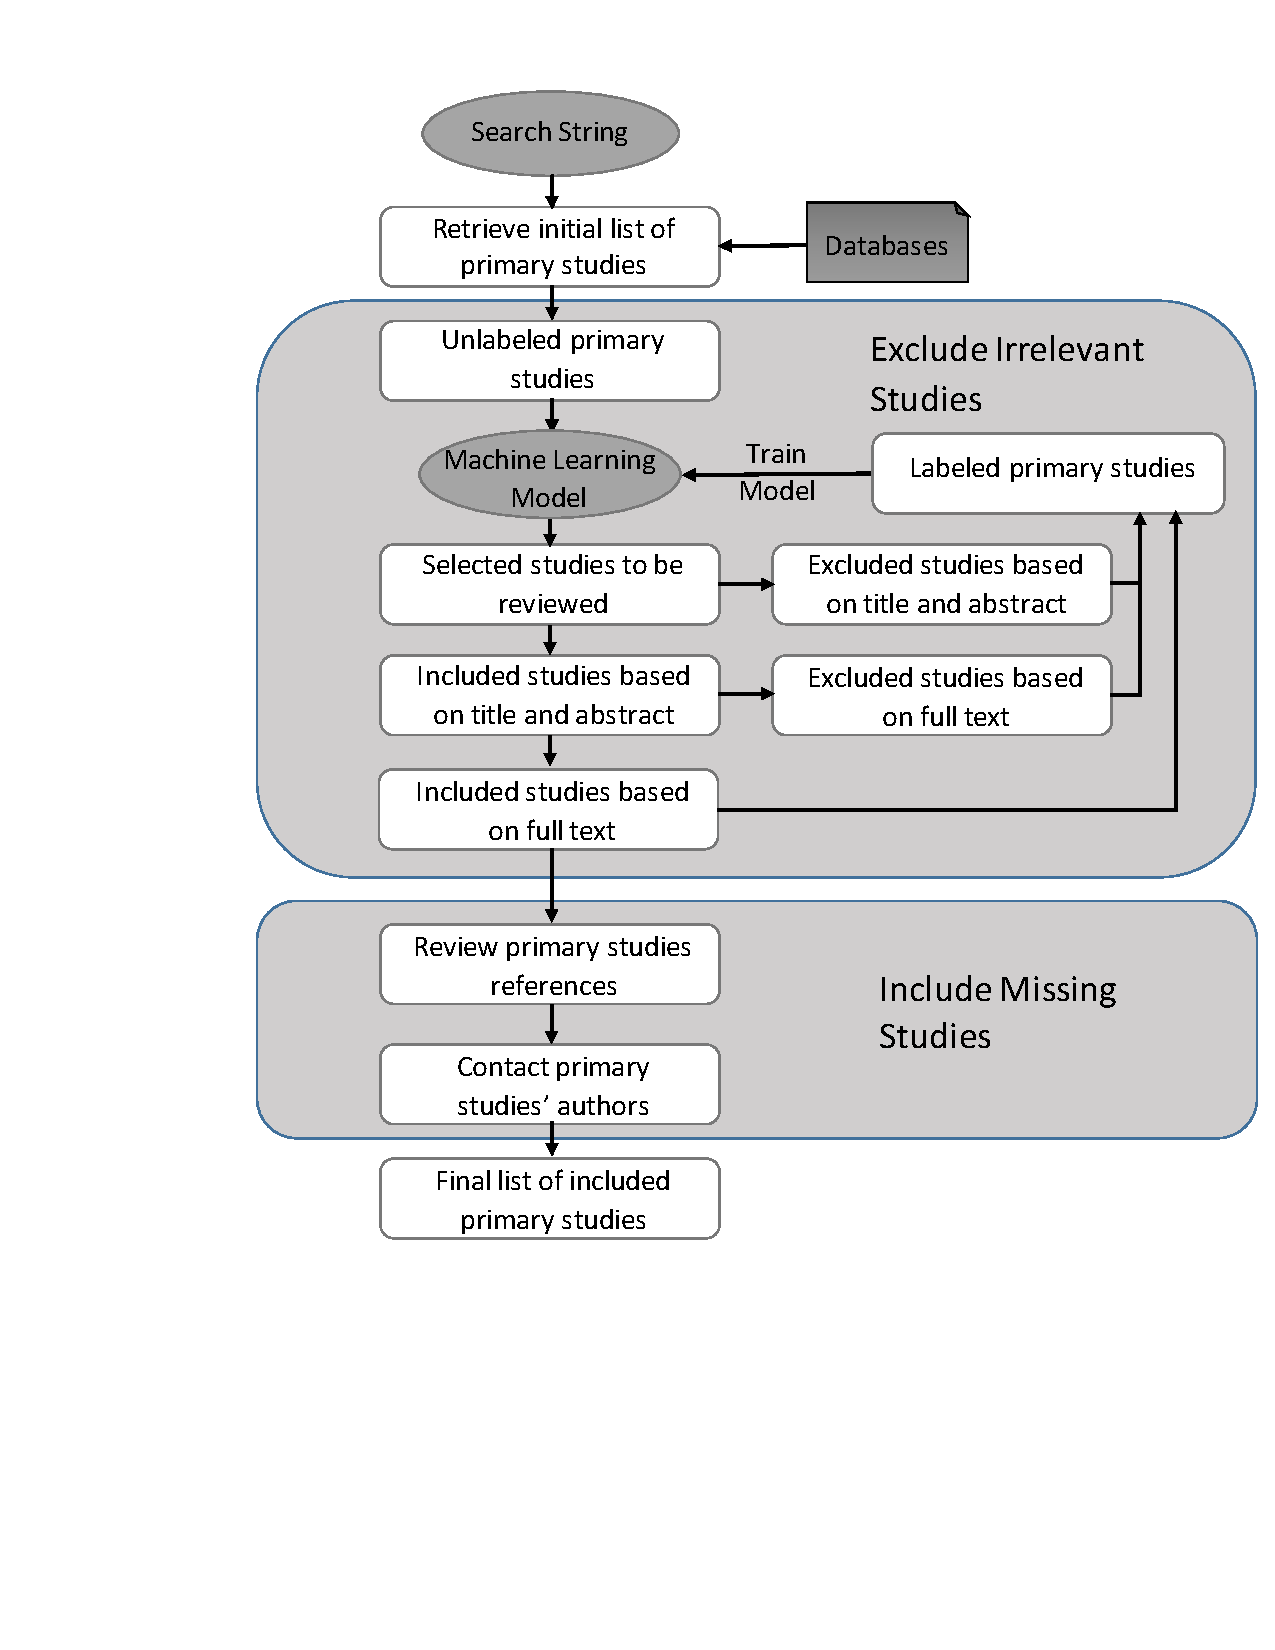
\includegraphics[width=0.6\linewidth]{Learning_based_primary_study_selection.pdf}
    \caption{Human-in-the-loop Primary study selection.}
    \label{fig: learning}
\end{figure}

\subsection{Human-in-the-loop Primary Study Selection}
\label{subsect: Learning based Primary Study Selection}


In contrast to the classical primary study procedures in Fig.~\ref{fig: prime}, with active learning as part of the process, the general form of human-in-the-loop primary study selection is presented in
Fig.~\ref{fig: learning}. Reviewers first review the title and abstract of the
suggested study, determine whether it is ``abstract relevant'' or ``abstract irrelevant''. If the study is relevant by title and abstract, the reviewer will then read the full text of the study and make the final decision-- ``content relevant'' or ``content irrelevant''. In the meantime, all the reviewed
studies will go into the training set. Note that only the title and abstract of the training set studies will be used to train the active learning model, thus making data extraction for training examples easy. Note that in this process, two-level relevance labels are generated and should be available to the active learning model. However, the fact is, for most of our datasets, ``abstract relevant'' labels are missing since they are not reported in the original SLR literature. As a result, only ``content relevant'' labels are being used for training in our experiments. In the rest of the paper, when we say ``relevant'', it means ``content relevant'' while ``irrelevant'' studies include every study that is not ``content relevant'' (``abstract relevant'' but ``content irrelevant'' or ``abstract irrelevant'').

The objective of Human-in-the-loop primary study selection (or machine learning
assisted citation screening or TAR) is different from that of common active
learning scenarios. Instead of trying to build a classifier as good as possible,
human-in-the-loop primary study selection seeks methods to retrieve most
``relevant'' studies with candidate studies reviewed as few as possible. This
difference in the objective leads to a different performance metrics (further explained in Section~\ref{subsect: Performance Metrics}) and thus
makes conventional active learning methods being outperformed by specially
designed methods like PAL~\cite{wallace2010semi}, Certainty plus Weighting~\cite{miwa2014reducing} in evidence-based
medicine and CAL~\cite{cormack2014evaluation,cormack2015autonomy} in
e-discovery.



\subsection{Algorithm Code}
\label{sect: Algorithm Code}

Differences of the three state-of-the-art active learning techniques for systematic reviews are from four aspects: 1) when to start training; 2) query strategy; 3) whether to stop training; 4) data balancing.

\begin{itemize}

\item
{\bf When to start training}: 

\textbf{P} stands for ``patient''. As suggested by Wallace et al.~\cite{wallace2010semi}, ``hasty generation'', which means start training with too few relevant examples, may leads to deteriorate performance. The algorithm keeps random sampling until a sufficient number of ``relevant'' studies retrieved. In our experiments, the sufficient number of ``relevant'' studies retrieved is set to $5$, which means when at least $5$ ``relevant'' studies have been retrieved by random sampling, the algorithm goes into next stage. PAL~\cite{wallace2010semi} and Certainty plus Weighting~\cite{miwa2014reducing} use \textbf{$P$} for when to start training.

\textbf{H} is the opposite. The algorithm stops random sampling as long as {\em ONE} ``relevant'' studies are retrieved, as suggested in CAL~\cite{cormack2014evaluation,cormack2015autonomy}.

\item
{\bf Query strategy}: 

\textbf{U} stands for ``uncertainty sampling''. The algorithm utilizes
uncertainty sampling to build the classifier, where unlabeled examples closest to the SVM decision plane are sampled for query. PAL~\cite{wallace2010semi} uses \textbf{U} for Query strategy.

\textbf{C} stands for ``certainty sampling''. The algorithm utilizes certainty sampling to build the classifier, where unlabeled examples furthest to the SVM decision plane and lie in the ``relevant'' side are sampled for query. Certainty plus Weighting~\cite{miwa2014reducing} and CAL~\cite{cormack2014evaluation,cormack2015autonomy} use \textbf{C} for query strategy.

\item
{\bf Whether to stop training}: 

\textbf{S} stands for ``stop training''. The algorithm stops training
once the classifier is stable. In our experiments, the classifier is treated as stable once more than $30$ ``relevant'' studies have been retrieved as training examples. PAL~\cite{wallace2010semi} uses \textbf{$S$} for whether to stop training.

\textbf{T} stands for ``continue training''. The algorithm never stops
training as suggested in CAL~\cite{cormack2014evaluation,cormack2015autonomy} and Certainty plus Weighting~\cite{miwa2014reducing}. If query strategy is \textbf{U}, algorithm switches to certainty sampling after classifier is stable but training never stops.

\item
{\bf Data balancing}: 

\textbf{N} stands for ``no data balancing''. The algorithm does not balance the training data as suggested by CAL~\cite{cormack2014evaluation,cormack2015autonomy}.

\textbf{A} stands for ``aggressive undersampling''. The algorithm utilizes aggressive undersampling when classifier is stable, as suggested by PAL~\cite{wallace2010semi}.

\textbf{W} stands for ``Weighting''. The algorithm utilizes Weighting for data balancing (before and after the classifier is stable), as suggested by Certainty plus Weighting~\cite{miwa2014reducing}.

\textbf{M} stands for ``mixing of Weighting and aggressive undersampling''. Weighting is applied before the classifier is stable while aggressive undersampling is applied after the classifier is stable. This treatment comes from the observation that ``Weighting'' performs good in early stages while ``aggressive undersampling'' performs good in late stages.

\end{itemize}
As a result, we ended up with 32 treatments including the state-of-the-art treatments as
\begin{itemize}
\item
\textbf{PUSA}: patient active learning~\cite{wallace2010semi,wallace2010active};
\item
\textbf{PCTW}: Certainty plus Weighting~\cite{miwa2014reducing};
\item
\textbf{HCTN}: continuous active learning~\cite{cormack2014evaluation,cormack2015autonomy}. 
\end{itemize}
All the 32 algorithms are tested and compared in Section~\ref{sect: Experiments}.

\section{Experiments}
\label{sect: Experiments}

This section describes the experimental procedures that we used to evaluate the treatments described in Section~\ref{sect: Algorithm Code} on the datasets described in Section~\ref{sect: datasets}. 

There is no human activity involved in these experiments, when asked for a label, the true label in the dataset is queried instead of a human reviewer. As a result, each experiment can be repeated with different random seed to capture variances and also makes reproducing the experiments possible. Each experiment is a simulation of one specific treatment on one dataset:

\begin{enumerate}
\item
Starts with an unlabeled collection of candidate studies, e.g. 8911 in Hall as shown in Table~\ref{tab: number}.

\item
\label{select}
Train a model on current labeled examples if enough labeled examples are available.

\item
Select $N=10$ studies based on the prediction of machine learning model on unlabeled examples for review. If no model is trained yet, random sample $N=10$ unlabeled studies.

\item
Query the true labels of the selected studies, i.e. 106 ``relevant'' and 8805 ``irrelevant'' in Hall as shown in Table~\ref{tab: number}, label them as their true labels.

\item
Go back to \ref{select} until finished.

\end{enumerate}


\subsection{Controlled Variables}
\label{subsect: Controlled Variables}

For the sake of a fair comparison, different treatments in Section~\ref{sect: Algorithm Code} share an identical set of controlled variables including preprocessing, featurization and classifier. 

\subsubsection{Preprocessing and Featurization}

Each candidate study in the initial list is first tokenized by stop words removal after concatenating its title and abstract. After tokenization, the bag of words are featurized into a term frequency vector. Then, reduce the dimensionality of the term frequency vector with to keep only $M=4000$ of the terms with highest tf-idf\footnote{For term $t$ in document $d$, $Tfidf(t, d)=w^t_d\times (\log \frac{|D|}{\sum_{d\in D} sgn(w^t_d)}+1)$ where $w^t_i$ is the term frequency of term $t$ in document $d$. For term $t$, $Tfidf(t) = \sum_{d\in D} Tfidf(t,d) = \sum_{d\in D} w^t_d \times (\log \frac{|D|}{\sum_{d\in D} sgn(w^t_d)}+1)$ and is used for feature selection.} score and normalize the hashed matrix by its L2 norm each row at last. TfidfVectorizer in scikit-learn is utilized for the above preprocessing and featurization steps. Alternatives such as stemming, LDA~\cite{blei2003latent}, paragraph vectors~\cite{le2014distributed} require exploration and are scheduled in our future works. 


\subsubsection{Classifier}

For this work we use a linear SVM as the classifier.
SVMs learn a hyperplane that separate relevant from irrelevant examples
in the training data. Linear SVMs do not make complicated assumptions about the data space and so are known to scale to very large, high-dimensional problems~\cite{joachims2006training}. Such linear SVMs are widely used in the state-of-the-art solutions~\cite{miwa2014reducing,cormack2015autonomy,wallace2010semi}. SVM's hyperplane is a natural tool for deciding what examples to show next to the human user. As discussed in Section~\ref{sect: Technical Briefing}, uncertainty sampling prefers the examples {\em closest} to the hyperplane boundary since these are the ones whose classification will
change, given small changes to the test data. On the other hand, certainty sampling prefers the examples with {\em highest} SVM predictions of being positive. SVC (set to be linear kernel) with default parameters in scikit-learn is utilized as the classifier.


\subsection{Performance Metrics}
\label{subsect: Performance Metrics}

Common active learning aims for building a better model with less training. Therefore, its performance metrics is usually some \textbf{accuracy, precision, recall} on the model prediction vs \textbf{training size} curve. The \textbf{accuracy, precision, recall} are measured on some validation set.

On the other hand, since the goal of human-in-the-loop primary study selection described in Section~\ref{subsect: Learning based Primary Study Selection} is different from that of common active learning, the performance metrics is also different. In human-in-the-loop primary study selection, the performance of each algorithm is evaluated by its \textbf{recall} vs. \textbf{studies reviewed} curve. The \textbf{recall} here is not a measurement on the trained model, but the number of ``relevant'' studies retrieved over the total number of ``relevant'' studies. An algorithm is better than the other if it can retrieve more ``relevant'' studies with fewer studies reviewed. This performance metrics is suggested by~\cite{cormack2015autonomy,cormack2014evaluation,tredennick2015} and best fits the objective of human-in-the-loop primary study selection. To enable a statistical analysis of the performances, the \textbf{recall} vs. \textbf{studies reviewed} curve is cut by a $0.95$ \textbf{recall} line and \textbf{studies reviewed} when reaching $0.95$ \textbf{recall} is used to assess performances. The reason behind $0.95$ \textbf{recall} is that a) $1.00$ \textbf{recall} can never be guaranteed by any text mining method unless all the candidate studies are reviewed; b) $0.95$ \textbf{recall} is usually considered acceptable in evidence-based medicine~\cite{cohen2011performance,cohen2006reducing,o2015using} despite the fact that there might still be ``relevant'' studies missing~\cite{shemilt2016use}. As a result, two numbers are recorded during experiments:
\begin{itemize}
\item
X95 = $\min \{x | r(x)\geq0.95 R\}$
\item
WSS@95 = $0.95-\text{X95}/T$
\end{itemize}
where in a total number of $T$ candidate studies, $R$ of them are ``relevant'' according to true labels, and $r(x)$ is the number of ``relevant'' studies found when $x$ studies have been reviewed.

Each treatment on each dataset is tested for 30 repeats\footnote{It is suggested that usually a sampling size of $30$ is adequate~\cite{isotalo2001basics}.} with random seeds ranging from 0 to 29. The 30 records collected for each treatment on each dataset are then used for comparison through Scott-Knott analysis as recommended by Mittas \& Angelis in their 2013 IEEE TSE paper~\cite{mittas2013ranking}. Scott-Knott clusters methods with little difference in performance together and rank each cluster with the median performances~\cite{scott1974cluster}. Since the 30 records for each treatment on each dataset do not follow a normal distribution, we utilize nonparametric hypothesis tests. Scott-Knott decides two methods are not of little difference if both bootstrapping~\cite{efron1982jackknife} and an effect size test~\cite{cliff1993dominance} agreed that the difference is statistically significant ($99\%$
confidence) and not a “negligible” effect (Cliff's Delta $\ge$ 0.147).





\subsection{Results}
\label{subsect: Results}


\begin{table*}
\caption{Scott-Knott analysis for number of studies reviewed/ work saved over sampling to reach $95\%$ recall}
\label{tab: scottknott}


\begin{center}
\parbox{.49\linewidth}{
\centering
{\scriptsize \begin{tabular}{l@{~~~}l@{~~~}r@{~~~}r@{~~~}r@{~~~}r}
\arrayrulecolor{lightgray}
\multicolumn{2}{l}{\textbf{Wahono}}  & \multicolumn{2}{c}{\textbf{X95}} & \multicolumn{2}{c}{\textbf{WSS@95}}\\\hline
\textbf{Rank} & \textbf{Treatment} & \textbf{Median} & \textbf{IQR} & \textbf{Median} & \textbf{IQR} \\\hline
\rowcolor{green!40}
  1 &         HUTM &    670  &  230 & 0.85 & 0.04 \\
  1 &         HCTM &    740  &  220 & 0.84 & 0.03 \\
\hline  2 &         HUTA &    780  &  140 & 0.84 & 0.02 \\
  2 &         HCTW &    790  &  90 & 0.84 & 0.02 \\
  2 &         HUTW &    800  &  110 & 0.84 & 0.02 \\
  2 &         HCTA &    800  &  140 & 0.83 & 0.02 \\
\hline  3 &         PCTM &    1150  &  450 & 0.78 & 0.07  \\
  3 &         PUTM &    1180  &  420 & 0.78 & 0.07 \\
  3 &         PCTA &    1190  &  340 & 0.78 & 0.05 \\
  3 &         PUTA &    1190  &  340 & 0.78 & 0.05 \\
\rowcolor{red!30}
  3 &         PCTW &    1210  &  350 &  0.78 & 0.06 \\
  3 &         PUTW &    1220  &  370 &  0.77 & 0.06 \\
\hline  4 &         HUSM &    1410  &  400 & 0.75 & 0.06 \\
\hline  5 &         HUSA &    1610  &  370 & 0.72 & 0.07 \\
\hline  6 &         PUSM &    1810  &  370 & 0.69 & 0.06 \\
\rowcolor{red!30}
  6 &         PUSA &    1910  &  700 & 0.67 & 0.10 \\
\hline  7 &         HUSW &    2220  &  400 & 0.63 & 0.06 \\
  7 &         PUSW &    2240  &  360 & 0.63 & 0.06 \\
\hline  8 &         HUTN &    2700  &  40 & 0.56 & 0.01 \\
\rowcolor{red!30}
  8 &         HCTN &    2720  &  40 & 0.56 & 0.01 \\
  8 &         PCSW &    2860  &  1320 & 0.54 & 0.20 \\
  8 &         PCSM &    2860  &  1320 & 0.54 & 0.20 \\
  8 &         PCTN &    2850  &  1130 & 0.54 & 0.17 \\
  8 &         PUTN &    2850  &  1130 & 0.54 & 0.17 \\
\hline  9 &         PCSN &    3020  &  1810 & 0.51 & 0.26 \\
  9 &         PCSA &    3020  &  1810 & 0.51 & 0.26 \\
\hline 10 &         HUSN &    4320  &  110 &  0.33 & 0.03 \\
 10 &         PUSN &    4370  &  1290 & 0.32 & 0.19 \\
 \rowcolor{blue!50}
\hline 11 &       linear &    6650  &  0 & 0 & 0 \\
 11 &         HCSA &    6490  &  2760 & -0.01 & 0.39 \\
 11 &         HCSN &    6490  &  2760 & -0.01 & 0.39 \\
 11 &         HCSM &    6490  &  3110 & -0.01 & 0.44 \\
 11 &         HCSW &    6490  &  3110 & -0.01 & 0.44 \\
\hline \end{tabular}}
}
\parbox{.49\linewidth}{
\centering
{\scriptsize \begin{tabular}{l@{~~~}l@{~~~}r@{~~~}r@{~~~}r@{~~~}r}
\arrayrulecolor{lightgray}
\multicolumn{2}{l}{\textbf{Hall}}  & \multicolumn{2}{c}{\textbf{X95}} & \multicolumn{2}{c}{\textbf{WSS@95}}\\\hline
\textbf{Rank} & \textbf{Treatment} & \textbf{Median} & \textbf{IQR} & \textbf{Median} & \textbf{IQR} \\\hline
  1 &         HUTW &    350  &  80 & 0.91 & 0.01 \\
  1 &         HUTA &    360  &  140 & 0.91 & 0.02 \\
  \rowcolor{green!40}
  1 &         HUTM &    360  &  140 & 0.91 & 0.02 \\
  1 &         HCTW &    370  &  50 & 0.91 & 0.01 \\
\hline  2 &         HCTM &    400  &  90 & 0.90 & 0.01 \\
  2 &         HCTA &    410  &  140 & 0.90 & 0.02 \\
  2 &         HUTN &    430  &  100 & 0.90 & 0.01 \\
  \rowcolor{red!30}
  2 &         HCTN &    460  &  70 & 0.90 & 0.01 \\
\hline  3 &         HUSM &    630  &  160 & 0.88 & 0.03 \\
\rowcolor{red!30}
  3 &         PCTW &    640  &  190 & 0.88 & 0.02 \\
  3 &         PUTW &    640  &  220 & 0.88 & 0.03 \\
\hline  4 &         PCTN &    680  &  210 & 0.87 & 0.03 \\
  4 &         PUTN &    680  &  200 & 0.87 & 0.03 \\
  4 &         PUTM &    690  &  230 & 0.87 & 0.03 \\
  4 &         PCTA &    730  &  260 & 0.87 & 0.03 \\
  4 &         PCTM &    720  &  230 & 0.87 & 0.03 \\
  4 &         PUTA &    730  &  230 & 0.87 & 0.03 \\
\hline  5 &         HUSW &    790  &  320 & 0.86 & 0.04 \\
  5 &         HUSA &    790  &  200 & 0.86 & 0.03 \\
  5 &         PUSW &    840  &  280 & 0.86 & 0.03 \\
  5 &         PUSM &    860  &  320 & 0.85 & 0.04 \\
  \rowcolor{red!30}
  5 &         PUSA &    970  &  310 & 0.84 & 0.04 \\
\hline  6 &         PCSW &    1560  &  580 & 0.77 & 0.07 \\
  6 &         PCSM &    1560  &  580 & 0.77 & 0.07 \\
\hline  7 &         PUSN &    1680  &  1390 & 0.76 & 0.18 \\
  7 &         PCSN &    1990  &  690 & 0.72 & 0.09 \\
  7 &         PCSA &    1990  &  690 & 0.72 & 0.09 \\
\hline  8 &         HUSN &    2270  &  1230 & 0.69 & 0.16 \\
\hline  9 &         HCSA &    7500  &  5170 & 0.03 & 0.58 \\
  9 &         HCSN &    7500  &  5170 & 0.03 & 0.58 \\
   \rowcolor{blue!50}
  9 &       linear &    8464  &  0 & 0 & 0 \\
  9 &         HCSM &    8840  &  5340 & -0.04 & 0.60 \\
  9 &         HCSW &    8840  &  5340 & -0.04 & 0.60 \\
\hline \end{tabular}}
}


\parbox{.49\linewidth}{
\centering
{\scriptsize \begin{tabular}{l@{~~~}l@{~~~}r@{~~~}r@{~~~}r@{~~~}r}
\arrayrulecolor{lightgray}
\multicolumn{2}{l}{\textbf{Radjenovi{\'c}}}  & \multicolumn{2}{c}{\textbf{X95}} & \multicolumn{2}{c}{\textbf{WSS@95}}\\\hline
\textbf{Rank} & \textbf{Treatment} & \textbf{Median} & \textbf{IQR} & \textbf{Median} & \textbf{IQR} \\\hline
\rowcolor{green!40}
  1 &         HUTM &    680   &  180  & 0.83 & 0.03 \\
  1 &         HCTM &    780   &  130  & 0.82 & 0.02 \\
  1 &         HCTA &    790   &  180  & 0.82 & 0.03 \\
  1 &         HUTA &    800   &  180  & 0.82 & 0.03 \\
\hline  2 &         HUSA &    890   &  310  & 0.80 & 0.06 \\
  2 &         HUSM &    890   &  270  & 0.80 & 0.05 \\
\hline  3 &         HUTW &    960   &  80  & 0.79 & 0.02 \\
  3 &         HCTW &    980   &  60  & 0.79 & 0.01 \\
  3 &         HUSW &    1080   &  410  & 0.77 & 0.07 \\
\hline  4 &         PCTM &    1150   &  270  & 0.76 & 0.05 \\
  4 &         PUTM &    1150   &  270  & 0.76 & 0.05 \\
\hline  5 &         HUTN &    1250   &  100  &  0.74 & 0.02 \\
  5 &         PCTA &    1260   &  210  & 0.74 & 0.05 \\
  5 &         PUTA &    1260   &  210  & 0.74 & 0.05 \\
  \rowcolor{red!30}
  5 &         HCTN &    1270   &  70  & 0.74 & 0.02 \\
  5 &         PUSM &    1250   &  400  & 0.74 & 0.07 \\
  5 &         PUSW &    1250   &  450  & 0.73 & 0.08 \\
  5 &         PUTW &    1350   &  310  & 0.72 & 0.06 \\
\rowcolor{red!30}
  5 &         PCTW &    1370   &  310  & 0.72 & 0.06 \\
  \rowcolor{red!30}
  5 &         PUSA &    1400   &  490  & 0.71 & 0.09 \\
\hline  6 &         HUSN &    1570   &  300  & 0.69 & 0.05 \\
  6 &         PCTN &    1600   &  360  & 0.68 & 0.06 \\
  6 &         PUTN &    1600   &  360  & 0.68 & 0.06 \\
\hline  7 &         PUSN &    1890   &  320  &  0.64 & 0.06 \\
\hline
  8 &         PCSW &    2250   &  940  & 0.57 & 0.20 \\
  8 &         PCSM &    2250   &  940  & 0.57 & 0.20 \\
\hline  9 &         PCSN &    2840   &  1680  & 0.47 & 0.31 \\
  9 &         PCSA &    2840   &  1680  & 0.47 & 0.31 \\
\hline 10 &         HCSA &    5310   &  2140  & 0.07 & 0.36 \\
 10 &         HCSN &    5310   &  2140  & 0.07 & 0.36  \\
 10 &         HCSM &    5320   &  2200  &  0.02 & 0.37  \\
 10 &         HCSW &    5320   &  2200  & 0.02 & 0.37 \\
 \rowcolor{blue!50}
 10 &       linear &    5700   &  0  & 0 & 0 \\
\hline \end{tabular}}}
\parbox{.49\linewidth}{
\centering
{\scriptsize \begin{tabular}{l@{~~~}l@{~~~}r@{~~~}r@{~~~}r@{~~~}r}
\arrayrulecolor{lightgray}
\multicolumn{2}{l}{\textbf{Kitchenham}}  & \multicolumn{2}{c}{\textbf{X95}} & \multicolumn{2}{c}{\textbf{WSS@95}}\\\hline
\textbf{Rank} & \textbf{Treatment} & \textbf{Median} & \textbf{IQR} & \textbf{Median} & \textbf{IQR} \\\hline
\rowcolor{green!40}
  1 &         HUTM &    760  &  170 & 0.50 & 0.14 \\
  1 &         HUTA &    840  &  100 & 0.46 & 0.06 \\
  1 &         PUTM &    850  &  180 & 0.45 & 0.11 \\
  1 &         PCTM &    860  &  130 & 0.44 & 0.09 \\
\hline  2 &         HCTA &    900  &  190 & 0.42 & 0.14 \\
  2 &         PCTA &    930  &  170 & 0.40 & 0.11 \\
  2 &         HCTM &    930  &  130 & 0.40 & 0.08 \\
  2 &         PUTA &    930  &  170 & 0.40 & 0.11 \\
\hline  3 &         PUSW &    1140  &  250 & 0.27 & 0.15 \\
  3 &         PUSM &    1140  &  250 & 0.27 & 0.15 \\
  3 &         HUTW &    1160  &  10 & 0.27 & 0.01 \\
  3 &         HCTW &    1180  &  40 & 0.25 & 0.03 \\
  \rowcolor{red!30}
  3 &         PCTW &    1190  &  170 & 0.25 & 0.10 \\
  3 &         PUTW &    1190  &  170 & 0.25 & 0.10 \\
\hline  4 &         HUSW &    1200  &  150 & 0.24 & 0.10 \\
  4 &         HUSM &    1200  &  150 & 0.24 & 0.10 \\
  4 &         HUSN &    1250  &  220 & 0.21 & 0.14 \\
  4 &         HUSA &    1250  &  220 & 0.21 & 0.14 \\
  \rowcolor{red!30}
  4 &         PUSA &    1250  &  290 & 0.21 & 0.19 \\
  4 &         PUSN &    1250  &  290 & 0.21 & 0.19 \\
  4 &         HUTN &    1260  &  10 & 0.21 & 0.01 \\
  \rowcolor{red!30}
  4 &         HCTN &    1280  &  30 & 0.20 & 0.02 \\
  4 &         PUTN &    1280  &  260 & 0.19 & 0.16 \\
  4 &         PCTN &    1290  &  260 & 0.19 & 0.15 \\
\hline  5 &         PCSW &    1370  &  260 & 0.14 & 0.22 \\
  5 &         PCSM &    1370  &  260 & 0.14 & 0.22 \\
  5 &         PCSN &    1400  &  340 & 0.12 & 0.22 \\
  5 &         PCSA &    1400  &  340 & 0.12 & 0.22 \\
\rowcolor{blue!50}
\hline  6 &       linear &    1615  &  0 & 0 & 0 \\
\hline  7 &         HCSA &    1670  &  90 & -0.03 & 0.05 \\
  7 &         HCSN &    1670  &  90 & -0.03 & 0.05 \\
  7 &         HCSM &    1670  &  90 & -0.03 & 0.05 \\
  7 &         HCSW &    1670  &  90 & -0.03 & 0.05 \\
\hline \end{tabular}}}

\end{center}
{\footnotesize Simulations are repeated for $30$ times, medians ($50$th percentile) and iqrs (($75$-$25$)th percentile) are presented. Smaller/larger median value for X90/WSS@95 represents better performance while smaller iqr means better stability. Treatments with same rank have no significant difference in performance while treatments of smaller number in rank are significantly better than those of larger number in rank. The recommended treatment FASTREAD is colored in {\setlength{\fboxsep}{1pt}\colorbox{green!40}{green}} while the state-of-the-art treatments are colored in {\setlength{\fboxsep}{1pt}\colorbox{red!30}{red}} and linear review is colored in {\setlength{\fboxsep}{1pt}\colorbox{blue!50}{blue}}.}


\end{table*}



\begin{table*}
\caption{Experimental results rearranged as blocks to compare the effectiveness of each code}
\label{tab: blockings}
\begin{center}
\parbox{.49\linewidth}{
\centering
\subfloat[64 blocks for RQ2.1 (T/S)]{
\label{tab: TS}
{\scriptsize \begin{tabular}{l@{~~~}|c@{~~~}c@{~~~}c@{~~~}c}
\arrayrulecolor{lightgray}
\textbf{T/S} & \multicolumn{4}{c}{\textbf{Scott-Knott Rank}} \\\hline
\textbf{Treatment} & \textbf{Wahono} & \textbf{Hall} & \textbf{Radjenovi{\'c}} & \textbf{Kitchenham} \\\hline
HUTM & \cellcolor{green!40} 1 & \cellcolor{green!40}1 & \cellcolor{green!40}1 & \cellcolor{green!40}1\\
HUSM & 4 & 3 & 2 & 4\\
\hline
HUTA &\cellcolor{green!40} 2 &\cellcolor{green!40} 1 &\cellcolor{green!40} 1 &\cellcolor{green!40} 1\\
HUSA & 5 & 5 & 2 & 4\\
\hline
HUTW &\cellcolor{green!40} 2 &\cellcolor{green!40} 1 & 3 &\cellcolor{green!40} 3\\
HUSW & 7 & 5 & 3 & 4\\
\hline
HUTN &\cellcolor{green!40} 8 &\cellcolor{green!40} 2 &\cellcolor{green!40} 5 & 4\\
HUSN & 10 & 8 & 6 & 4\\
\hline
HCTM &\cellcolor{green!40} 1 &\cellcolor{green!40} 2 &\cellcolor{green!40} 1 &\cellcolor{green!40} 2\\
HCSM & 11 & 9 & 10 & 7\\
\hline
HCTA &\cellcolor{green!40} 2 &\cellcolor{green!40} 2 &\cellcolor{green!40} 1 &\cellcolor{green!40} 2\\
HCSA & 11 & 9 & 10 & 7\\
\hline
HCTW &\cellcolor{green!40} 2 &\cellcolor{green!40} 1 &\cellcolor{green!40} 3 &\cellcolor{green!40} 3\\
HCSW & 11 & 9 & 10 & 7\\
\hline
HCTN &\cellcolor{green!40} 8 &\cellcolor{green!40} 2 &\cellcolor{green!40} 5 &\cellcolor{green!40} 4\\
HCSN & 11 & 9 & 10 & 7\\
\hline
PUTM &\cellcolor{green!40} 3 &\cellcolor{green!40} 4 &\cellcolor{green!40} 4 &\cellcolor{green!40} 1\\
PUSM & 6 & 5 & 5 & 3\\
\hline
PUTA &\cellcolor{green!40} 3 &\cellcolor{green!40} 4 & 5 & \cellcolor{green!40}2\\
PUSA & 6 & 5 & 5 & 4\\
\hline
PUTW &\cellcolor{green!40} 3 & \cellcolor{green!40}3 & 5 & 3\\
PUSW & 7 & 5 & 5 & 3\\
\hline
PUTN & \cellcolor{green!40}8 &\cellcolor{green!40} 4 &\cellcolor{green!40} 6 & 4\\
PUSN & 10 & 7 & 7 & 4\\
\hline
PCTM & \cellcolor{green!40}3 &\cellcolor{green!40} 4 &\cellcolor{green!40} 4 &\cellcolor{green!40} 1\\
PCSM & 8 & 6 & 8 & 5\\
\hline
PCTA & \cellcolor{green!40}3 &\cellcolor{green!40} 4 & \cellcolor{green!40}5 &\cellcolor{green!40} 2\\
PCSA & 9 & 7 & 9 & 5\\
\hline
PCTW & \cellcolor{green!40}3 &\cellcolor{green!40} 3 &\cellcolor{green!40} 5 &\cellcolor{green!40} 3\\
PCSW & 8 & 6 & 8 & 5\\
\hline
PCTN & \cellcolor{green!40}8 &\cellcolor{green!40} 4 & \cellcolor{green!40}6 & \cellcolor{green!40}4\\
PCSN & 9 & 7 & 9 & 5\\
\hline
\end{tabular}}
}}
\parbox{.49\linewidth}{
\centering
\subfloat[64 blocks for RQ2.2 (U/C)]{
\label{tab: UC}
{\scriptsize \begin{tabular}{l@{~~~}|c@{~~~}c@{~~~}c@{~~~}c}
\arrayrulecolor{lightgray}
\textbf{U/C} & \multicolumn{4}{c}{\textbf{Scott-Knott Rank}} \\\hline
\textbf{Treatment} & \textbf{Wahono} & \textbf{Hall} & \textbf{Radjenovi{\'c}} & \textbf{Kitchenham} \\\hline
HUTM & 1 & \cellcolor{green!40}1 & 1 & \cellcolor{green!40}1\\
HCTM & 1 & 2 & 1 & 2\\
\hline
HUTA & 2 &\cellcolor{green!40} 1 & 1 &\cellcolor{green!40} 1\\
HCTA & 2 & 2 & 1 & 2\\
\hline
HUTW & 2 & 1 & 3 & 3\\
HCTW & 2 & 1 & 3 & 3\\
\hline
HUTN & 8 & 2 & 5 & 4\\
HCTN & 8 & 2 & 5 & 4\\
\hline
HUSM & \cellcolor{green!40}4 &\cellcolor{green!40} 3 & \cellcolor{green!40}2 &\cellcolor{green!40} 4\\
HCSM & 11 & 9 & 10 & 7\\
\hline
HUSA &\cellcolor{green!40} 5 & \cellcolor{green!40}5 & \cellcolor{green!40}2 & \cellcolor{green!40}4\\
HCSA & 11 & 9 & 10 & 7\\
\hline
HUSW & \cellcolor{green!40}7 & \cellcolor{green!40}5 &\cellcolor{green!40} 3 &\cellcolor{green!40} 4\\
HCSW & 11 & 9 & 10 & 7\\
\hline
HUSN &\cellcolor{green!40} 10 &\cellcolor{green!40} 8 &\cellcolor{green!40} 6 &\cellcolor{green!40} 4\\
HCSN & 11 & 9 & 10 & 7\\
\hline
PUTM & 3 & 4 & 4 & 1\\
PCTM & 3 & 4 & 4 & 1\\
\hline
PUTA & 3 & 4 & 5 & 2\\
PCTA & 3 & 4 & 5 & 2\\
\hline
PUTW & 3 & 3 & 5 & 3\\
PCTW & 3 & 3 & 5 & 3\\
\hline
PUTN & 8 & 4 & 6 & 4\\
PCTN & 8 & 4 & 6 & 4\\
\hline
PUSM & \cellcolor{green!40}6 & \cellcolor{green!40}5 &\cellcolor{green!40} 5 &\cellcolor{green!40} 3\\
PCSM & 8 & 6 & 8 & 5\\
\hline
PUSA &\cellcolor{green!40} 6 &\cellcolor{green!40} 5 & \cellcolor{green!40}5 &\cellcolor{green!40} 4\\
PCSA & 9 & 7 & 9 & 5\\
\hline
PUSW &\cellcolor{green!40} 7 &\cellcolor{green!40} 5 &\cellcolor{green!40} 5 &\cellcolor{green!40} 3\\
PCSW & 8 & 6 & 8 & 5\\
\hline
PUSN & \cellcolor{blue!50}10 & 7 & \cellcolor{green!40}7 &\cellcolor{green!40} 4\\
PCSN & 9 & 7 & 9 & 5\\
\hline
\end{tabular}}
}}

\parbox{.49\linewidth}{
\centering
\subfloat[64 blocks for RQ2.3 (H/P)]{
\label{tab: HP}
{\scriptsize \begin{tabular}{l@{~~~}|c@{~~~}c@{~~~}c@{~~~}c}
\arrayrulecolor{lightgray}
\textbf{H/P} & \multicolumn{4}{c}{\textbf{Scott-Knott Rank}} \\\hline
\textbf{Treatment} & \textbf{Wahono} & \textbf{Hall} & \textbf{Radjenovi{\'c}} & \textbf{Kitchenham} \\\hline
HUTM &\cellcolor{green!40} 1 &\cellcolor{green!40} 1 & \cellcolor{green!40}1 & 1\\
PUTM & 3 & 4 & 4 & 1\\
\hline
HUTA &\cellcolor{green!40} 2 &\cellcolor{green!40} 1 &\cellcolor{green!40} 1 &\cellcolor{green!40} 1\\
PUTA & 3 & 4 & 5 & 2\\
\hline
HUTW & \cellcolor{green!40}2 & \cellcolor{green!40}1 &\cellcolor{green!40} 3 & 3\\
PUTW & 3 & 3 & 5 & 3\\
\hline
HUTN & 8 & \cellcolor{green!40}2 & \cellcolor{green!40}5 & 4\\
PUTN & 8 & 4 & 6 & 4\\
\hline
HUSM &\cellcolor{green!40} 4 & \cellcolor{green!40}3 & \cellcolor{green!40}2 &\cellcolor{blue!50} 4\\
PUSM & 6 & 5 & 5 & 3\\
\hline
HUSA &\cellcolor{green!40} 5 & 5 & \cellcolor{green!40}2 & 4\\
PUSA & 6 & 5 & 5 & 4\\
\hline
HUSW & 7 & 5 & \cellcolor{green!40}3 &\cellcolor{blue!50} 4\\
PUSW & 7 & 5 & 5 & 3\\
\hline
HUSN & 10 &\cellcolor{blue!50} 8 &\cellcolor{green!40} 6 & 4\\
PUSN & 10 & 7 & 7 & 4\\
\hline
HCTM &\cellcolor{green!40} 1 &\cellcolor{green!40} 2 &\cellcolor{green!40} 1 & \cellcolor{blue!50}2\\
PCTM & 3 & 4 & 4 & 1\\
\hline
HCTA & \cellcolor{green!40}2 & \cellcolor{green!40}2 &\cellcolor{green!40} 1 & 2\\
PCTA & 3 & 4 & 5 & 2\\
\hline
HCTW &\cellcolor{green!40} 2 & \cellcolor{green!40}1 &\cellcolor{green!40} 3 & 3\\
PCTW & 3 & 3 & 5 & 3\\
\hline
HCTN & 8 &\cellcolor{green!40} 2 & \cellcolor{green!40}5 & 4\\
PCTN & 8 & 4 & 6 & 4\\
\hline
HCSM & \cellcolor{blue!50}11 & \cellcolor{blue!50}9 & \cellcolor{blue!50}10 &\cellcolor{blue!50} 7\\
PCSM & 8 & 6 & 8 & 5\\
\hline
HCSA &\cellcolor{blue!50} 11 &\cellcolor{blue!50} 9 &\cellcolor{blue!50} 10 &\cellcolor{blue!50} 7\\
PCSA & 9 & 7 & 9 & 5\\
\hline
HCSW & \cellcolor{blue!50}11 & \cellcolor{blue!50}9 & \cellcolor{blue!50}10 & \cellcolor{blue!50}7\\
PCSW & 8 & 6 & 8 & 5\\
\hline
HCSN & \cellcolor{blue!50}11 &\cellcolor{blue!50} 9 & \cellcolor{blue!50}10 & \cellcolor{blue!50}7\\
PCSN & 9 & 7 & 9 & 5\\
\hline
\end{tabular}}
}}
\parbox{.49\linewidth}{
\centering
\subfloat[32 blocks for RQ2.4 (M/A/W/N)]{
\label{tab: MAWN}
{\scriptsize \begin{tabular}{l@{~~~}|c@{~~~}c@{~~~}c@{~~~}c}
\arrayrulecolor{lightgray}
\textbf{M/A/W/N} & \multicolumn{4}{c}{\textbf{Scott-Knott Rank}} \\\hline
\textbf{Treatment} & \textbf{Wahono} & \textbf{Hall} & \textbf{Radjenovi{\'c}} & \textbf{Kitchenham} \\\hline
HUTM & \cellcolor{green!40}1 & 1 & 1 & 1\\
HUTA & 2 & 1 & 1 & 1\\
HUTW & 2 & 1 & 3 & 3\\
HUTN & 8 & 2 & 5 & 4\\
\hline
HUSM & \cellcolor{green!40}4 &\cellcolor{green!40} 3 & 2 & 4\\
HUSA & 5 & 5 & 2 & 4\\
HUSW & 7 & 5 & 3 & 4\\
HUSN & 10 & 8 & 6 & 4\\
\hline
HCTM &\cellcolor{green!40} 1 & \cellcolor{blue!50}2 & 1 & 2\\
HCTA & 2 & 2 & 1 & 2\\
HCTW & 2 & 1 & 3 & 3\\
HCTN & 8 & 2 & 5 & 4\\
\hline
HCSM & 11 & 9 & 10 & 7\\
HCSA & 11 & 9 & 10 & 7\\
HCSW & 11 & 9 & 10 & 7\\
HCSN & 11 & 9 & 10 & 7\\
\hline
PUTM & 3 &\cellcolor{blue!50} 4 & \cellcolor{green!40}4 &\cellcolor{green!40} 1\\
PUTA & 3 & 4 & 5 & 2\\
PUTW & 3 & 3 & 5 & 3\\
PUTN & 8 & 4 & 6 & 4\\
\hline
PUSM & 6 & 5 & 5 & 3\\
PUSA & 6 & 5 & 5 & 4\\
PUSW & 7 & 5 & 5 & 3\\
PUSN & 10 & 7 & 7 & 4\\
\hline
PCTM & 3 & \cellcolor{blue!50}4 & \cellcolor{green!40}4 &\cellcolor{green!40} 1\\
PCTA & 3 & 4 & 5 & 2\\
PCTW & 3 & 3 & 5 & 3\\
PCTN & 8 & 4 & 6 & 4\\
\hline
PCSM & 8 & 6 & 8 & 5\\
PCSA & 9 & 7 & 9 & 5\\
PCSW & 8 & 6 & 8 & 5\\
PCSN & 9 & 7 & 9 & 5\\
\hline
\end{tabular}}
}}
\end{center}
{\footnotesize Each subtable compares one pair of algorithm codes by rearranging the results from Table~\ref{tab: scottknott} so that codes other than the ones to be compared with are identical within each block. Smaller number in rank means better performance while same number in rank means no significant difference in performance. All the blocks where the suggested code performs significantly better than its alternatives are colored in {\setlength{\fboxsep}{1pt}\colorbox{green!40}{green}} while all the blocks where the suggested code is outperformed by any other code are colored in {\setlength{\fboxsep}{1pt}\colorbox{blue!50}{blue}}. Results are summarized as following: (a) {\setlength{\fboxsep}{1pt}\colorbox{green!40}{58}}/{\setlength{\fboxsep}{1pt}\colorbox{blue!50}{0}}; (b) {\setlength{\fboxsep}{1pt}\colorbox{green!40}{34}}/{\setlength{\fboxsep}{1pt}\colorbox{blue!50}{1}}; (c) {\setlength{\fboxsep}{1pt}\colorbox{green!40}{30}}/{\setlength{\fboxsep}{1pt}\colorbox{blue!50}{20}}; (d) {\setlength{\fboxsep}{1pt}\colorbox{green!40}{8}/\colorbox{blue!50}{3}}.
}
\end{table*}


{\bf RQ1: Can active learning techniques reduce cost in primary study selection?} 

In Table~\ref{tab: scottknott}, we tested 32 active learning treatments and linear review. According to the results, most active learning treatments perform consistently better than linear review (colored in {\setlength{\fboxsep}{1pt}\colorbox{blue!50}{blue}}) on all four datasets while four treatments (\textbf{HCS*}) can be even worse than linear review. Interestingly these four treatments share same codes of \textbf{HCS}, which hastily start training (\textbf{H}) with greedy query strategy (\textbf{C}) and give up the attempt to correct the model short after (\textbf{S}). The problem of ``hasty generation'' is maximized in the setting of \textbf{HCS} and thus leads to an even worse performance than linear review. In general, other active learning treatments can reduce review costs by allowing the reviewer to read fewer studies while still find 95\% of the relevant ones.

\begin{lesson}
    In general, active learning techniques can reduce cost in primary study selections with a sacrifice of (say 5\%) recall.
\end{lesson}




{\bf RQ2: Should we just adopt the state-of-the-art treatments from other fields? Is it possible to build a better one by mixing and matching from those?}

The performance of the three state-of-the-art treatments are colored in {\setlength{\fboxsep}{1pt}\colorbox{red!30}{red}}. On Wahono and Kitchenham datasets, Certainty plus Weighting (\textbf{PCTW}) outperforms the other two treatments; while on Hall dataset, CAL (\textbf{HCTN}) has the best performance; and on Radjenovi{\'c} dataset, all three treatments perform similarly. PAL (\textbf{PUSA}) seems to be dominated by Certainty plus Weighting (\textbf{PCTW}) but this does not mean techniques in PAL are not useful. In fact, neither of the three state-of-the-art treatments has ever ranked highest (rank 1) in any dataset. This means that adopting the state-of-the-art treatments will not produce best results. According to Scott-Knott analysis, the performance of one treatment, \textbf{HUTM} (colored in {\setlength{\fboxsep}{1pt}\colorbox{green!40}{green}}), consistently stays in the top rank across all four datasets. Before asserting that \textbf{HUTM} is our preferred treatment, let us analyze the effectiveness of each algorithm code.

\textbf{RQ2.1}: Stop training or not?

Table~\ref{tab: TS} rearranges the results such that in each block, only the code for whether to stop training are different (\textbf{T} vs. \textbf{S}). Across the $4\times 16 = 64$ blocks, \textbf{T} (continue training) performs significantly better than \textbf{S} (stop training) in 58 blocks and performs similarly to \textbf{S} in the rest 6 blocks. Therefore, \textbf{T} dominates\footnote{We say Code A dominates Code B if in every block, A performs no worse than B and in some blocks A performs significantly better than B.} \textbf{S}. Although training time can be saved by \textbf{S}, it sacrifices the performance and the ability to adapt. So no, never stop training.

\textbf{RQ2.2}: Which query strategy is more effective?

Table~\ref{tab: UC} rearranges the results so that in each block, only the code for query strategy are different (\textbf{U} vs. \textbf{C}). Across the $4\times 16 = 64$ blocks, \textbf{U} (uncertainty sampling) performs significantly better than \textbf{C} (certainty sampling) in 34 blocks while the other way around in 1 blocks. Overall, \textbf{U} performs better than \textbf{C} and if only considering the $4\times 8 = 32$ \textbf{T} blocks, \textbf{U} dominates \textbf{C}. Therefore, uncertainty sampling is suggested for query strategy in early stages especially if \textbf{T} continue training is applied.

\textbf{RQ2.3}: When to start training?

Table~\ref{tab: HP} rearranges the results so that in each block, only the code for when to start training are different (\textbf{H} vs. \textbf{P}). Across the $4\times 16 = 64$ blocks, \textbf{H} (hasty, start training with 1 ``relevant'' example) performs significantly better than \textbf{P} (patient, start training with at least 5 ``relevant'' examples) in 30 blocks while the other way around in 20 blocks. No clear winners from the overall view. However, if only considering the $4\times 4 = 16$ \textbf{UT} blocks, \textbf{H} dominates \textbf{P}. Therefore, \textbf{H} starting training with 1 ``relevant'' example is suggested if \textbf{U} uncertainty sampling and \textbf{T} continue training are applied.

\textbf{RQ2.4}: Which data balancing method is most effective?

Table~\ref{tab: MAWN} rearranges the results so that in each block, only the code for data balancing are different (\textbf{M}, \textbf{A}, \textbf{W}, or \textbf{N}). Across the $4\times 8 = 32$ blocks, \textbf{M} (Weighting plus aggressive undersampling) performs significantly better than the rest in 8 blocks while \textbf{W} (Weighting) performs significantly better than the rest in 3 blocks. Overall, a) \textbf{N} (no data balancing) is dominated by any data balancing method in every block; b) \textbf{M} dominates other codes on Wahono, Radjenovi{\'c}, and Kitchenham datasets; c) \textbf{W} dominates other codes on Hall datasets; d) across all $4$ blocks of \textbf{HUT}, \textbf{M} dominates other codes. To conclude, data balancing methods are effective; \textbf{M} Weighting plus aggressive undersampling is suggested if \textbf{U} uncertainty sampling and \textbf{T} continue training are applied and \textbf{H} training starts with 1 ``relevant'' example.

As indicated in the answers for \textbf{RQ2.1-2.4}, \textbf{UT} are definitely better than their alternatives while \textbf{H} and \textbf{M} are conditionally better given the selection of other codes. Together, it forms our recommended treatment \textbf{HUTM}, which 
\begin{enumerate}
\item
randomly samples from unlabeled candidate studies until 1 ``relevant'' example retrieved;
\item
then start training with Weighting and query with uncertainty sampling, until 30 ``relevant'' examples retrieved;
\item
then train with aggressive undersampling and query with certainty sampling until finished.
\end{enumerate}

This treatment is named as FASTREAD. According to Table~\ref{tab: scottknott}, FASTREAD (\textbf{HUTM}) consistently shows in the first rank across all four datasets and significantly outperforms all three state-of-the-art treatments.

\begin{lesson}
    No, we should not just adopt the state-of-the-art methods from other fields. A better method called FASTREAD is generated by mixing and matching from the state-of-the-art methods.
\end{lesson}

\begin{table}
\caption{How much can FASTREAD save?}
\label{tab: save}
\begin{center}
\begin{tabular}{ |l|c|c|c|}
  \hline
   Datasets & \# Studies Reviewed & Review Cost & \# Relevant Studies \\
  \hline
  Wahono & $7002-670=6332$ & $\geq6332C_A+4C_D$ & 4\\
  \hline
  Hall & $8991-360=8631$ & $\geq8611C_A+6C_D$ & 6\\
  \hline
  Radjenovi{\'c} & $6000-680=5320$ & $\geq5320C_A+3C_D$ & 3\\
  \hline
  Kitchenham & $1704-760=944$ & $32C_D+944C_A$ & 3\\
  \hline
%   Kitchenham (abstract) & 334 & $6C_D+334C_A$ & -1\\
%   \hline
\end{tabular}
\end{center}
{\footnotesize Numbers of reviewing every candidate study minus numbers of reviewing with FASTREAD. For example, on Kitchenham dataset, FASTREAD reviews 944 fewer studies, which costs $32C_D+944C_A$ less review effort, while misses 3 ``relevant'' ones. Here $C_D$ is the cost to review a study by its content and $C_A$ is the cost to review a study by its title and abstract.}
\end{table}

\textbf{RQ3: How much effort can FASTREAD save in an SLR?}

In terms of the number of studies reviewed, WSS@95 scores in Tabel~\ref{tab: scottknott} reflects how much FASTREAD can save. Number of ``relevant'' studies ($|R|$) and the total number of candidate studies ($|C|$) affect WSS@95 a lot, e.g. WSS@95=0.50 in Kitchenham dataset with $|R|$=44, $|C|$=1704 and WSS@95=0.91 in Hall dataset with $|R|$=106, $|C|$=8911. Even the smallest number of WSS@95=0.50 in Kitchenham dataset is a success in the reduction of number of studies need to be reviewed comparing to the 5\% recall lost.

In terms of the actual review cost,
%FASTREAD
%saves less since the most burdensome part-- reviewing studies by their content can not be reduced much. On Kitchenham dataset, reviewing every candidate study costs $132C_D+1704C_A$ while with FASTREAD, the cost can be reduced to $100C_D+760C_A$. 
Table~\ref{tab: save} shows how much FASTREAD save over reviewing all candidate studies. Suppose $C_D=9C_A$, following the estimation that Shemilt made: 1 minute to screen a title-abstract record, 4 minutes to retrieve a full-text study report, and 5 minutes to screen a full-text study report~\cite{shemilt2016use}. Then the reduction in review cost is $(32C_D+944C_A)/(132C_D+1704C_A) = 42.6\%$\footnote{According to Table~\ref{tab: number}, reviewing all studies costs $132C_D+1704C_A$. In our simulations, in average FASTREAD did 760 abstract reviews and 100 content reviews.}. On other datasets, although we do not have the exact number of ``abstract relevant'' studies, we can estimate the worst case review cost reduction\footnote{In the worst case we assume that every study reviewed is ``abstract relevant'' and thus costs $C_D+C_A$ to review and there is no ``abstract relevant'' study left except for the 5\% missing ``content relevant'' ones. E.g. in Wahono dataset, FASTREAD reviews 670 studies among the 7002 candidate ones, it costs $670(C_A+C_D)$ while reviewing all studies costs $(670+4)C_D+7002C_A$.} with the numbers in Table~\ref{tab: number} and Table~\ref{tab: save}: a) Wahono dataset: $1-670(C_A+C_D)/((670+4)C_D+7002C_A) = 48.7\%$; b) Hall dataset: $1-360(C_A+C_D)/((360+6)C_D+8991C_A) = 70.7\%$; c) Radjenovi{\'c} dataset: $1-680(C_A+C_D)/((680+3)C_D+6000C_A) = 44.0\%$. 
Note that training time costs are negligibly small (1 second for each round in average) compared to the review time $C_A$ because of the small training size (less than 1000 examples before reaching 95\% recall). 
%Utilizing two levels of relevance labels to minimize the review cost is planned in our future works when datasets with the required labels are available.

\begin{lesson}
    Our results and estimations suggest that FASTREAD can save around $40\%$ review cost while retrieving $95\%$ of the ``relevant'' studies.
\end{lesson}

Note that if the reader doubts the value of a 40\% reduction the review cost, they are reminded that that overall cost may be days to weeks to months. Hence, the reductions achieved by FASTREAD are of much practical benefit.





\section{Tool Support}
\label{sect: tool}

\begin{figure*}[!tbhp]
    \centering
    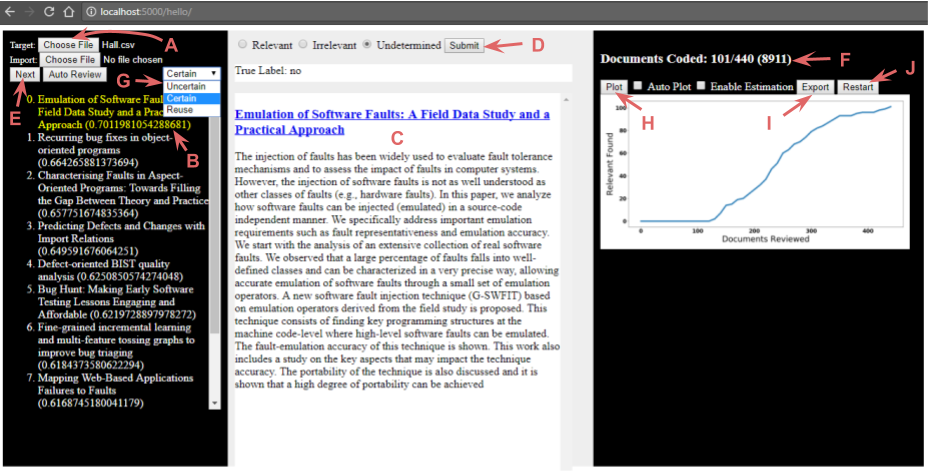
\includegraphics[width=\linewidth]{FASTREAD.png}
    \caption{Basic interface of the FASTREAD tool.}
    \label{fig:FASTREAD}
\end{figure*}


\begin{figure*}[!tbhp]
    \centering
    \subfloat[Input format]
    {
        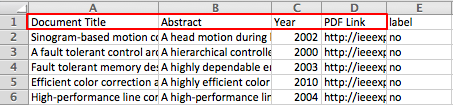
\includegraphics[width=0.48\linewidth]{Input.png}\label{fig:input}
    }
    \subfloat[Output format]
    {
        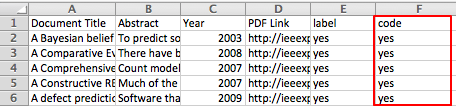
\includegraphics[width=0.48\linewidth]{Output.png}\label{fig:output}
    }    
    
    \caption{Data format for FASTREAD tool.}
    \label{fig:csv}
\end{figure*}

In order to implement FASTREAD, we developed a simple tool as shown in Fig.~\ref{fig:FASTREAD}. This software is freely available from SeaCraft Zenodo at \textit{https://doi.org/10.5281/zenodo.837861} and its Github repository at \textit{https://github.com/fastread/src}. 


Using FASTREAD, a review starts with \textbf{A}: selecting the input candidate study list from \textit{workspace/data/} directory. The input candidate list is specified in the format shown in Fig.~\ref{fig:input}. The input CSV file must have the \textit{Document Title}, \textit{Abstract}, \textit{Year}, and \textit{PDF Link} columns. The \textit{label} column, which is the true label of the candidate studies, is optional and is only used for testing. The output CSV file generated by the FASTREAD tool has an additional \textit{code} column, which is the reviewer-decided label for the candidate study. The final inclusion list can be retrieved by extracting all the studies with ``yes'' in the \textit{code} column.

The review then proceeds as follows:
\begin{enumerate}
\item[\textbf{B}] Randomly select $10$ candidate studies for review.
\item[\textbf{C}] Read through the title and abstract (and click on the title and read the full text if needed) of the candidate study.
\item[\textbf{D}] Decide whether this study should be coded as \textit{Relevant} or \textit{Irrelevant} and click the \textit{Submit} button.
\item[\textbf{E}] Click the \textit{Next} button and the codes are saved. Another $10$ candidate studies will be selected for review.
\item[\textbf{F}] The review status will change every time new studies are coded by reviewer and the \textit{Next} button is hit. The status is shown in the format ``Documents Coded: \textit{Number of relevant studies found} / \textit{Number of studies reviewed} (\textit{Total number of candidate studies}).''
\item[\textbf{G1}] Once \textbf{1} ``relevant'' study is coded, \textit{Random sampling} will be replaced by \textit{Uncertainty sampling}.
\item[\textbf{G2}] Once \textbf{30} ``relevant'' study is coded, \textit{Uncertainty sampling} can be changed to \textit{Certainty sampling}.
\item[\textbf{H}] Fig. can be plotted by clicking the \textit{Plot} button or checking \textit{Auto Plot}. The generated figure can also be found in the \textit{src/static/image/} directory. The new figure will overwrite any old one.
\item[\textbf{I}] Once finished, coded studies can be exported into a CSV file in the \textit{workspace/coded/} directory, in the format shown in Fig.~\ref{fig:output}.
\end{enumerate}

Note that the \textit{Restart} button (\textbf{J}) is only for testing and discards all codes.



\section{Threats to Validity}
\label{sect: Threats to Validity}

There are several validity threats to the design of this study~\cite{feldt2010validity}. Any conclusions made from this work must be considered with the following issues in mind:

{\em Conclusion validity} focuses on the significance of the treatment. To
enhance the conclusion validity of this work, we employed several statistical
tests (Scott-Knot) to reduce the changes of making spurious conclusions. 

{\em Internal validity} focuses on how sure we can be that the treatment
actually caused the outcome. To enhance our internal validity,
as far as possible, we heavily constrained our experiments
(see  our simulated in strictly controlled environments as discussed in Section~\ref{subsect: Controlled Variables}).

{\em Construct validity} focuses on the relation between the theory
behind the experiment and the observation. In this work, we evaluated
our results via different treatments with WSS@95 as stated in Section~\ref{subsect: Performance Metrics}-- note that those
measures took us as close as we can to computing
cost reduction without ``abstract relevant'' information. 
That is, it fits the objective of human-in-the-loop primary study selection as defined in the current literature~\cite{tredennick2015,cormack2015autonomy,cormack2014evaluation}. Increasing the number of different measures may increase construct validity
so, in future work, we will further explore more metrics.

{\em External validity }concerns how well the conclusion can be applied outside. All the conclusions in this study are drawn from the experiments running on three software engineering SLR datasets created with information from Hall, Wahono, Radjenovi{\'c} et al. studies~\cite{hall2012systematic,wahono2015systematic,radjenovic2013software} and one dataset provided by Kitchenham~\cite{kitchenham2010systematic}. Therefore, such conclusions may not be applicable to datasets of different scenarios, e.g., citation screening from evidence based medicine or TAR from e-discovery. Such bias threatens any classification experiment. The best any researcher can do is to document that bias then make available to the general research community all the materials used in a study (with the hope that other researchers will explore similar work on different datasets). Existing active learning techniques in citation screening have been criticized by Olorisade et al. for being not replicable~\cite{olorisade2016critical,olorisade2017reproducibility}. To this end, we have published all our code at \textit{https://github.com/fastread/src} and all our data at \textit{https://doi.org/10.5281/zenodo.837298}.

In the experiments, we assume that the human reviewer is always correct. In practice, this assumption cannot hold and problems such as disagreement between reviewers or concept drift (in which reviewers disagree with themselves as time passes) may occur.  As discussed
below when we discuss {\em Future Work}, we intend to explore this matter in the near future.

The comparisons in our experiment are based on the controlled variables listed in Section~\ref{subsect: Controlled Variables}. The conclusion in Section~\ref{subsect: Results} may become unreliable if any of the controlled variables changes.



\section{Conclusions}\label{sect: Conclusion}

Systematic literature reviews are the primary method for aggregating evidence in evidence-based software engineering. It is suggested for every researcher in software engineering to frequently conduct SLRs in~\cite{keele2007guidelines}. The hugest barrier to accomplish this is the cost. Usually an SLR would take months to finish and the conclusion drawn can be out of date in a few years. To tackle this barrier, this study focuses on primary study selection, one of the most difficult and time consuming steps in an SLR. Machine learning methods, especially active learning, are explored in our attempts to reduce the effort required to exclude primary studies. Three state-of-the-art active learning methods, two from evidence-based medicine and one from e-discovery, are analyzed and tested. In our experiments, we showed that by decomposing and reassembling the state-of-the-art treatments, a new treatment can be created which outperforms the state-of-the-art treatments and achieves a large cost reduction with 5\% recall lost.  

This work has lead to a simple software tool called FASTREAD, which
we described above in Section~\ref{sect: tool}. We are currently advertising
that tool on social media and hope that, very soon,
we will be  able to report on
case studies when other researchers use this tool. FASTREAD is
an open source tool, published in Github, and we also hope
that FASTREAD will be maintained and improved by numerous 
researchers exploring this kind of technology. 

\section{Future Work}
This study has several limitations as described in Section~\ref{sect: Frequently Asked Questions} and \ref{sect: Threats to Validity}. We plan to address those limitations in future work. Specific problems and plans for the future are listed below.

\begin{itemize}

\item
{\em Conclusions are drawn from three synthetic SLR datasets and one Kitchenham dataset.} Validate the generalizability of the results on different datasets, including datasets from evidence-based medicine and e-discovery.

\item
{\em Experiment results are evaluated by WSS@95, which assumes a stop rule of reaching 95\% recall.} How to stop at 95\% recall without first knowing the number ``relevant'' studies in the pool is an interesting topic. We are exploring this topic actively.

\item
{\em The size and prevalence of data can affect performance of FASTREAD.} The analysis of such effects may in return help estimate the prevalence, therefore makes it possible to estimate the total number of ``relevant'' studies in the pool.

\item
{\em About $10\%$ to $20\%$ efforts are spent on random selection step and most of the variances are also introduced in this step.} To speed up the random selection step, external expert knowledge will be introduced while unsupervised learning methods such as VTM or LDA will also be considered in future work. 

\item
{\em Some magic parameters are arbitrarily chosen, which may affect the performance.} However, parameter tuning is not a good fit for human-in-the-loop primary study selection because a) parameters should be tuned for the data working on; b) but the effect of applying different parameters can not be tested since querying extra label incurs extra cost. Therefore, novel methods should be explored for parameter selection; e.g. better criterion for when to switch from uncertainty sampling to certainty sampling (instead of the ``30'' relevant examples rule applied now).


\item
{\em Current scenario is restricted to having only one reviewer, which is impractical in practice.} Problems including how to assign review tasks to multiple reviewers and how to utilize reviewers with different cost and different capability will be explored in the future.

\item
{\em Current scenario assumes that reviewers never make mistakes, which is definitely not true in practice.} How to tackle concept drift (reviewers disagree with themselves) and how to settle disagreements (reviewers disagree with each other) would be valuable contributions for future work.

\item
{\em This study focuses only on primary study selection.} Assists on other steps of SLR such as searching, data extraction, and protocol development can also help reduce total effort of SLRs. The potential of combining VTM, snowballing, and other tools with FASTREAD needs to be explored as well.


\end{itemize}

 We invite other researchers to join us in the exploring the above. To that end, we have made all our tools and scripts readily available, on-line).

% With all the work in this study, a baseline result for human-in-the-loop primary study selection has now been established. There are still many concerns and potential improvements on FASTREAD, as discussed in Section~\ref{sect: Frequently Asked Questions}. We will keep working on the future work items and we believe that with all the materials in this work published, SE researchers can also explore further in SLR cost reduction. With our best hope, the effort required for conducting SLRs will eventually be reduced to days of work in the future and thus enable researchers to conduct SLRs much more frequently.

\section*{Acknowledgement}
The authors thank Barbara Kitchenham for
her attention to this work and for
sharing with us the ``Kitchenham'' dataset used in our experiments.
 
% \bibliographystyle{plain}
\bibliographystyle{spmpsci}
% \bibliography{sigproc} 
\input{R1arxiv.bbl}








\end{document}











\end{document}











\end{document}











\end{document}


